\documentclass[12pt]{report}

\usepackage[a4paper,margin=2.5cm]{geometry}
\usepackage{tabularx}
\usepackage{longtable}
\usepackage{fancyvrb}
\usepackage{booktabs}
\usepackage{xcolor}
\usepackage{newfloat}
\usepackage{graphicx}
\usepackage[pdftex]{hyperref}
\usepackage{amsmath}
\usepackage{tikz}
\usetikzlibrary{positioning,shapes,shadows,arrows}
\usetikzlibrary{calc}

\newcommand{\smallHead}[1]{\vspace{1ex}\noindent\textbf{#1}\nopagebreak\par}
\newcommand{\Format}{\smallHead{Format}}
\newcommand{\Operands}{\smallHead{Operands}}
\newcommand{\Operand}{\smallHead{Operand}}
\newcommand{\Example}{\smallHead{Example}}
\newcommand{\Arguments}{\smallHead{Arguments}}
\newcommand{\Argument}{\smallHead{Argument}}
\newcommand{\ReturnValue}{\smallHead{Return Value}}
\newcommand{\Clauses}{\smallHead{Clauses}}
\newcommand{\Clause}{\smallHead{Clause}}
\newcommand{\ct}{{\normalfont\tt{\^}}}
\renewcommand{\it}[1]{\textit{#1}}
\renewcommand{\tt}[1]{\texttt{#1}}
\newcommand{\co}[1]{\texttt{#1}}
\newenvironment{note}
  {\begin{quote}\textbf{Note:}}
  {\end{quote}}
\DeclareFloatingEnvironment{example}
\definecolor{rwp-color}{RGB}{0,1,149}

\makeatletter
\newenvironment{exampl}[1][\unskip]
  {\refstepcounter{example}%
    \par\addvspace{0.5\baselineskip}
    \@beginparpenalty=10000
    Example \theexample: #1
    \list{}{\listparindent=0pt%
      \itemindent\listparindent%
      \rightmargin=\leftmargin%
      \topsep=0pt%
      \parsep\z@\@plus\p@}%
  \item\relax}
  {\endlist\par\addvspace{0.5\baselineskip}}
\newcommand{\RWP}{\textcolor{rwp-color}{RuleWorks> }}
\definecolor{cmd-color}{RGB}{149,0,0}
\newcommand{\cmd}[1]{\textcolor{cmd-color}{#1}}
\makeatother

\renewenvironment{quote}
  {\list{}{\leftmargin=1.5em\topsep=1ex\rightmargin=\leftmargin}\item\relax}
  {\endlist}

\parindent=0cm
\parskip=1ex

\hypersetup{
    colorlinks,
    citecolor=black,
    filecolor=black,
    linkcolor=[RGB]{0 8 80},
    urlcolor=black
}

\begin{document}

\begin{titlepage}
  \newgeometry{left=7.5cm}
  \noindent
  {\huge\textbf{\textsf{RuleWorks}}}\\[1em]
  \makebox[0pt][l]{\rule{1.3\textwidth}{1pt}}
  \par
  \vfill
  \noindent
  {\LARGE\textsf{User's Guide}}
  \vskip\baselineskip
  \noindent
  % \textsf{August 2008}
\end{titlepage}

\restoregeometry

\tableofcontents

\chapter{Introduction}
\label{c:intro}

RuleWorks is a rules-based programming language that represents an
evolutionary step beyond OPS5. The major features of RuleWorks are
listed below:

\begin{itemize}
\item Improved data representation
\begin{itemize}
\item inheritance hierarchy
\item working memory can be partitioned
\end{itemize}
\item Improved program modularity
  \begin{itemize}
  \item programs can be divided into independent, or dependent,
    modular subsystems
  \item rules-based modules can easily be called, and can return a
    value
  \end{itemize}
\item Portable implementation supporting numerous platforms
\end{itemize}

OPS5 is a rules-based programming language that was used most often to
develop knowledge-based and expert systems. It was created at Carnegie
Mellon University in the late 1970s and early 1980s by Charles Forgy,
John McDermott, the late Allen Newell, and Mike Rychener. Publication
of Forgy's OPS5 User's Manual in 1981 established a commonly used
standard for the language. OPS5 is characterized by:

\begin{itemize}
\item A global database, called working memory.
\item Program statements called condition-action rules that match
  patterns in working memory and then perform actions that change
  working memory.
\item Execution order that is not procedural, but is driven by the
  data in working memory. The order in which rules are executed is
  controlled by the recognize-act cycle.
\item Computation with symbolic expressions and numbers.
\end{itemize}

\section{Sample Program}

Most of the examples in this guide are based on a sample program
called \tt{KIWI}, which solves the system configuration problems of a
hypothetical manufacturer, the Kiwi Computer Company. Kiwi Computer
Co. makes the computer parts shown in Table \ref{t:kiwi}. A customer
can order a Kiwi computer as a package or as separate parts. The
purpose of the \tt{KIWI} program is to help the Kiwi sales force
verify that the parts a customer has ordered can be assembled into a
working computer.

\begin{table}[h]
  \begin{tabularx}{\columnwidth}{lXr}
    \toprule
    Part Number &  Name &  Price (\$) \\
    \midrule
    KI-9200   & Kiwi-9200 CPU Base Unit & 999.95 \\
    MS-9200   & Kiwi-9200 Memory Card   & 129.95 \\
    FD-35     & 3.5-inch Floppy Disk Drive &  99.95 \\
    FD-525    & 5.25-inch Floppy Disk Drive & 109.95 \\
    HD-30     & 30-Megabyte Hard Disk Drive & 299.95 \\
    HD-200    & 200-Megabyte Hard Disk Drive & 599.95 \\
    TA-9200   & High-Performance Cartridge Tape & 399.95 \\
    KB-9200   & 108-Key Keyboard with Mouse Port &  99.95 \\
    MOUSE-1   & 100 pulses per inch Graphic Mouse & 59.95 \\
    VM-9200   & 19-inch B/W Alphanumeric Monitor &  99.95 \\
    CM-9200   & 21-inch Color Graphic Display System & 199.95 \\
    NI-9200   & Kiwi-9200 Network Interface &  39.95 \\
    S-OS-9200 & KIWOS Operating System & 9.95 \\
    S-WI-9200 & KiWindows Windows Software &  59.95 \\
    S-CA-9200 & KiwiCalc Spreadsheet Software  &  29.95 \\
    S-NE-9200 & KiwiTalk Network Software &  89.95 \\
    \bottomrule
  \end{tabularx}
  \caption{Parts Manufactured by Kiwi Computer Company}
  \label{t:kiwi}
\end{table}

\section{Working Memory}

\emph{Working memory} is a global, dynamic user workspace that
contains information about a problem and the current state of its
solution. Information is stored in \emph{working memory objects} that
are organized by \emph{class}.  Each working memory object (WMO,
pronounced ``wim-oh'') has a class name and a list of associated
\emph{attributes} and their values. The class name classifies the
object according to the type of information it contains. The
attributes and their values describe the object's characteristics. (In
database terms, object classes are like tables and attributes are like
fields).

The information in Table~\ref{t:kiwi} could be represented in working
memory by objects that are all instances of a single class, named
\tt{PART}. A better representation would use several classes to
capture more information about the differences between types of
parts. For example, most of the Kiwi parts are optional (a customer
can buy either a floppy disk drive or a hard disk drive) but one is
required (the base unit that contains the CPU). This distinction can
be represented by class \tt{OPTION} for the optional components and
class \tt{BOX} for the required CPU box.

RuleWorks allows object classes to be organized into an inheritance
hierarchy in which \emph{subclasses} inherit from a \emph{parent
  class}. In this example, \tt{OPTION} and \tt{BOX} are subclasses (or
\emph{descendants}) of the parent class \tt{PART} (see Figure~\ref{f:1-1}).

All parts made by Kiwi Computer Company have the following three
characteristics: a part number, a name, and a price. These
characteristics are represented by attributes whose names are
\tt{PART-NUMBER}, \tt{NAME}, and \tt{PRICE}. These attributes are
declared in object class \tt{PART} and are inherited by its
descendants.

\begin{figure}
  \centering
  \input f1-1.tex
  \caption{Class Hierarchy of Parts}
  \label{f:1-1}
\end{figure}

(Figure~\ref{f:1-1} shows only part of the class hierarchy used in the
sample program. For a complete illustration, see Figure 2-1)

Some of the optional parts are hardware; some are software. Hardware
and software have different characteristics and are therefore
separated into different classes with different attributes. For
example, a hardware component can take up a slot in the CPU box while
a software component does not.  Conversely, software is available on
different media (two sizes of floppy disk, or tape) while hardware is
not.

The software options can be further divided between applications and
the operating system. Kiwi Computer currently sells three
applications, so there are three subclasses of \tt{APPLICATION}. There
is currently only one subclass of \tt{OPERATING-SYSTEM}, but there may
be other supported operating systems in the future.

A sample object of class \tt{BOX} is shown below.  The first three
attributes are inherited from class \tt{PART} and have values from
Table~\ref{t:kiwi}. The last two attributes belong to class \tt{BOX}
only, because the box is the only part that has slots:

\begin{quote}
\begin{verbatim}
(box ^part-number ki-9200 ^name |Kiwi-9200 CPU Base Unit| 
     ^price 999.95 ^card-in-slot ^card-in-slot-obj-id)
\end{verbatim}
\end{quote}

The attribute names are preceded by a caret (\ct) to show that they
are references into the object.

\section{Rules}

Program statements in RuleWorks are condition-action (or ``if
\ldots{}then'') rules that operate on working memory. A \emph{rule}
has a name and consists of a condition part (called the
\emph{left-hand side} or LHS) and an action part (called the
\emph{right-hand side} or RHS). The LHS is separated from the RHS by
an arrow, created by typing two minus signs and a greater-than
sign. Figure~\ref{f:1-2} shows the format of a rule.

Rules express the requirements of the problem to be solved. For
example, one requirement of the Kiwi program is that a customer who
buys application software must also buy the \tt{KIWOS} operating
system. The rule shown in Example~\ref{e:samprule} enforces this
requirement. The left-hand side of the rule matches when the contents
of working memory do not meet the \tt{KIWOS} requirement; the
right-hand side of the rule takes corrective actions.

\begin{figure}[h]
  \centering
  
\includegraphics[scale=0.7]{f1-2}
  \caption{Format of a Rule}
  \label{f:1-2}
\end{figure}

\begin{example}[h]
\begin{quote}
\begin{verbatim}
(rule
    verify-configuration:application-needs-kiwos
    (active-context ^name verify-configuration)
    (kiwos-application ^$instance-of <applic>)
    -(kiwos)
  -->
    (write
        (crlf) |Caution: to run an application| <applic>
        (crlf) |you need to have KIWOS, but you don't have KIWOS.|
        (crlf) | Fixup: adding KIWOS to your order.|
        (crlf))
    (make error ^severity warning ^message |No operating system|)
    (make kiwos))
\end{verbatim}
\end{quote}
\caption{A Sample Rule}
\label{e:samprule}
\end{example}

\subsection{The Left-Hand Side}

The LHS is a series of patterns called \emph{condition elements} (CEs)
that are compared to objects during program execution.  RuleWorks
implicitly performs a logical AND operation on all the CEs on the
LHS. (In database terms, each CE is like a query against a table, and
the LHS is a like a join across the results of those queries.)

The LHS of the sample rule in Example~\ref{e:samprule} consists of
three CEs. The first CE is used to control the flow of execution of
the program. It states that the program must be in the "verify
configuration" phase of execution before this rule can \emph{fire} (be
executed).

The second CE states that an object of class \tt{KIWOS-APPLICATION} or
any of its subclasses exists in working memory. The customer order
could include any application: \tt{KiWindows}, \tt{KiwiCalc}, or
\tt{KiwiTalk}. Because subclasses inherit \emph{membership} in their
parent classes, objects of classes \tt{KIWINDOWS}, \tt{KIWICALC}, or
\tt{KIWITALK} match the class name \tt{KIWOS-APPLICATION} (see
Figure~\ref{f:1-1}). The second CE also binds (assigns a value to) the
variable \tt{<APPLIC>}.

The third CE is negated. It states that no object of class \tt{KIWOS}
exists.

\subsection{The Right-Hand Side}

The RHS is a series of actions that are taken when the rule is
executed. Actions are taken in the order you write them. An action
consists of an action name and its arguments; it usually manipulates
the contents of working memory.

The RHS of the sample rule in Example~\ref{e:samprule} contains three
actions. The \tt{WRITE} action displays a message to the user that the
order is being changed. The variable \tt{<APPLIC>} that was bound on
the LHS is used here on the RHS. The two \tt{MAKE} actions create new
objects of the classes \tt{ERROR} and \tt{KIWOS}, respectively. The
creation of the \tt{KIWOS} object changes the contents of working
memory such that the operating system requirement is met. Thus, this
rule will fire only once even if the customer orders all three
applications.

\section{Recognize-Act Cycle}

The recognize-act cycle is the pattern-matching procedure that takes
place repeatedly as a RuleWorks program executes (see
Figure~\ref{f:1-3}). The cycle consists of the following steps:

\begin{center}
  \begin{tabularx}{\columnwidth}{cX}
    \textbf{Match}  & Search working memory to find
                      all combinations of objects
                      that satisfy the condition  
                      elements in the left-hand sides 
                      of the program's rules. A rule 
                      name plus a combination of     
                      objects that satisfy that     
                      rule's condition elements is    
                      called an \emph{instantiation}. Place 
                      all instantiations in a list   
                      called the \emph{conflict set}. [In   
                      database terms, the conflict    
                      set is like a collection of the 
                      results of all the joins        
                      (left-hand sides) in the
                      program.] \\\addlinespace
    \textbf{Select} & Using an ordered sequence of  
                      criteria, take the             
                      instantiation with the highest 
                      priority out of the conflict    
                      set. If the conflict set is     
                      empty (because no left-hand     
                      side has been satisfied), the   
                      cycle stops. \\\addlinespace
    \textbf{Act}    & Execute the actions on the      
                      right-hand side of the rule in  
                      the selected instantiation,     
                      operating on the objects       
                      matched by its left-hand side. 
  \end{tabularx}
\end{center}

You can think of the match and select steps together as recognizing
which is the best rule to fire, thus the term recognize-act cycle.

\begin{figure}[h]
  \centering
  \input f1-3.tex
  \caption{Recognize-Act Cycle}
  \label{f:1-3}
\end{figure}

The cycle can stop after the select step, if the conflict set is
empty. It stops during the act step if a \tt{RETURN} or \tt{QUIT}
action is executed.

\section{Conflict Resolution}

The process by which the run-time system selects one instantiation
from the conflict set is called \emph{conflict resolution}. During
conflict resolution, the run-time system uses one of two possible
strategies to select the best instantiation, based on five different
criteria (see Table~\ref{t:crc}).

\begin{table*}[h]
  \def\arraystretch{1.2}
  \begin{tabularx}{\columnwidth}{lX}
    \toprule
    \textbf{Refraction}   & Select an instantiation 
                            only once.               
                            Refraction prevents       
                            programs from looping    
                            infinitely on the same   
                            data by removing         
                            instantiations from the 
                            conflict set after they 
                            have been selected.  \\
    \textbf{Recency}      & Select the instantiation 
                            that refers to the most  
                            recent information.      
                            Objects that have the    
                            highest time-tags contain
                            the most recent data.    
                            Therefore, the system    
                            selects the instantiation 
                            that contains the highest
                            time-tags.              \\
    \textbf{Class Specificity} & Select the instantiation 
                                 whose rule refers to the 
                                 most specific class      
                                 names.                   
                                 Class specificity is     
                                 determined by the        
                                 position of object       
                                 classes in the           
                                 inheritance hierarchy.  
                                 Top-level classes are    
                                 less specific than       
                                 low-level classes. For   
                                 example, a \tt{PART} object is 
                                 least specific; a        
                                 \tt{KIWINDOWS} object is most 
                                 specific. \\
    \textbf{Test Specificity} &  Select an instantiation 
                                of the rule whose        
                                left-hand side is the    
                                most specific.          
                                Test specificity is     
                                determined by the number 
                                of attribute-value tests 
                                in the rule's left-hand  
                                side. The rule whose     
                                left-hand side contains 
                                the most tests is the    
                                most specific. \\
    \textbf{Arbitrary choice} &  After all other criteria 
                                have been applied and   
                                more than one            
                                instantination remains,  
                                select one at random. \\
    \bottomrule
  \end{tabularx}
  \caption{Conflict Resolution Criteria}
  \label{t:crc}
\end{table*}

The RuleWorks run-time system supports two conflict-resolution
strategies: the lexicographic-sort (\tt{LEX}) strategy and the
means-ends-analysis (\tt{MEA}) strategy. The \tt{LEX} strategy applies
each selection criterion once, in the order shown in
Table~\ref{t:crc}. The \tt{MEA} strategy follows the same order, but
it applies recency in two steps. First it selects the instantiation(s)
whose first time-tag is most recent. It then selects from the
remaining instantiation(s) the one(s) whose combined time-tags are
most recent.

The sample program, \tt{KIWI}, uses the \tt{MEA} strategy to create a
control structure. The program divides the problem into tasks, creates
an object for each task, and places the condition element that matches
the control object first on each left-hand side (see Example 1-1). The
extra step of the \tt{MEA} strategy ensures that only instantiations
that match the most recent control object can fire.

The default strategy for RuleWorks is \tt{MEA}, and DIGITAL recommends
using this strategy for almost all applications. You can change the
strategy to \tt{LEX} with the \tt{STRATEGY} clause of the
\tt{ENTRY-BLOCK} declaration.

\section{Other Program Components}

In addition to rules, RuleWorks programs consist of block constructs,
declarations, optional \tt{ON-} statements, optional catchers, and
optional comments. Each program must have at least one entry block;
declaration blocks and rule blocks are optional. Inside an entry
block, program statements must be ordered as shown in
Figure~\ref{f:1-4}: declarations first, then \tt{ON-} statements (if
any), last rules and catchers.

\begin{figure}[h]
  \centering
  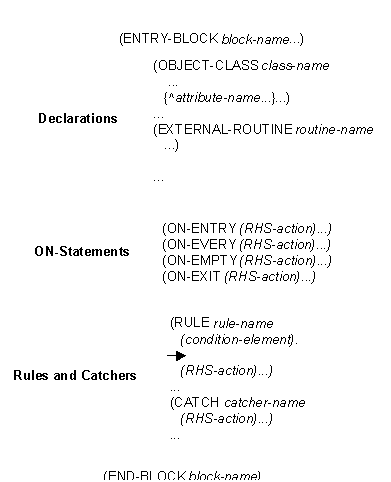
\includegraphics[scale=0.7]{f1-4}
  \caption{Format of a RuleWorks Program}
  \label{f:1-4}
\end{figure}

\subsection{Block Constructs}

RuleWorks provides block constructs for program and data
modularity. In OPS5, all rules were active and all of working memory
could be matched by any rule. In RuleWorks, the rules and WMOs of one
block can be isolated from those of every other block.

RuleWorks provides three block constructs:

\begin{tabularx}{\columnwidth}{lX}
    \toprule
    Name & Purpose \\
    \midrule
    \tt{ENTRY-BLOCK} & Makes an entry point
                       for your RuleWorks   
                       code so that it can  
                       be called from       
                       RuleWorks or other   
                       languages, accepting 
                       arguments and        
                       optionally returning 
                       a value. Objects     
                       whose class is       
                       declared inside an   
                       entry block can be   
                       matched by rules in  
                       that entry block     
                       only. \\\addlinespace
    \tt{DECLARATION-BLOCK} & Creates a collection
                             of object class and  
                             external routine     
                             declarations that    
                             can be shared among  
                             entry blocks.        
                             Objects whose class  
                             is declared inside a 
                             declaration block    
                             can be matched by    
                             rules in any entry   
                             or rule block that   
                             uses that            
                             declaration block. \\\addlinespace
    \tt{RULE-BLOCK} & Creates a collection
                      of rules that can be 
                      shared among entry   
                      blocks. Objects      
                      whose class is       
                      declared inside a    
                      rule block can be    
                      matched by rules in  
                      that rule block      
                      only. \\\addlinespace
    \bottomrule
  \end{tabularx}


Each block must end with an \tt{END-BLOCK} statement. See
Chapter~\ref{c:program} for more information on block constructs.

\subsection{Declarations}

Declarations are units of code that define the object classes and
external routines used in a program. Object class and external routine
declarations must precede any executable statement.

\subsection{\tt{ON-} Statements}

\tt{ON-} statements contain actions that are executed at particular
steps in the recognize-act cycle, without matching objects in working
memory. RuleWorks provides four \tt{ON-} statements:

\begin{center}
\begin{tabular}{ll}
    \toprule
    Name     & Time Executed               \\
    \midrule
    \tt{ON-ENTRY} & Before match step of first recognize-act cycle. \\
    \tt{ON-EVERY} & After act step of every cycle except the last one. \\
    \tt{ON-EMPTY} & After select step when the conflict set is empty. \\
    \tt{ON-EXIT}  & After act step of the last cycle.  \\
  \bottomrule
\end{tabular}
\end{center}

Like rules, \tt{ON-} statements must be enclosed in parentheses. They
must appear after declarations (if any) and before other executable
statements (that is, rules and catchers). For more information see
Chapter~\ref{c:program}.

\subsection{Catchers}

Catchers contain actions that are executed after a certain number of
recognize-act cycles have fired, without matching objects in working
memory. You specify the number of cycles in an \tt{AFTER} action. For
more information see Chapter~\ref{c:program}.

\subsection{Comments}

To improve the readability of your program, you can format units of
code by using white space (spaces, tabs, and new-line characters) and
comments. A comment starts with a semicolon and finishes at the end of
the same line. For example:

\begin{quote}
\begin{verbatim}
;This is a comment.
\end{verbatim}
\end{quote}

If you want more than one line of comment text, you must start each
line with a semicolon.

The compiler ignores the text of comments.  Therefore, comments can
contain any ASCII character and can start anywhere that a space
character is valid.

%%% Local Variables:
%%% mode: latex
%%% TeX-master: "rwug"
%%% End:

\chapter[Working Memory]{Knowledge Representation and 
  Working Memory}
\label{c:workingmem}

Working memory is the dynamic, global database which encodes
the problem a RuleWorks program is to solve and the current
state of the solution. Different aspects of the problem are
organized into different classes of information in working
memory. Classes which store related information can be
grouped into an inheritance hierarchy.

Each class contains a set of named attributes with their
associated attribute structure and default values. Attribute
structure is scalar (atomic) or multi-valued (compound). Each
instance of a class is called a working-memory object (WMO).

As a RuleWorks program runs, WMOs are continually created,
changed, and deleted. In OPS5, every rule in a program could
``see'' (potentially match, change, or delete) every object in
working memory. The advantage with RuleWorks is that when a
given entry block is executing, the rules in that block are
only able to see working memory which is in scope.

\section{Object Class Hierarchy}

RuleWorks allows classes directly to represent hierarchical
categories of data. Object classes can inherit attribute
names, attribute structure, and default values from a parent
class. A parent class can have many subclasses, but each
subclass can have only one immediate parent. This is called
single inheritance as opposed to multiple. You can think of
this graphically as a tree with branches and leaves. The
figure shows the inheritance tree of the object class \tt{PART} in
the sample program \tt{KIWI}.

Inheritance from a parent class is declared in the
\tt{INHERITS-FROM} clause of the \tt{OBJECT-CLASS} declaration of the
subclass:

\begin{quote}
\begin{verbatim}
(object-class subclass-name
    (inherits-from parent-class-name))
\end{verbatim}
\end{quote}
  
Because objects inherit membership in the parent class, objects match
condition elements not only of their own class, but also of their
\emph{ancestor} object classes (their parents, and their parents'
parents, and so on). Thus, a condition element can ask for an object
of a high-level class (such as \tt{OPTION}), and be matched by
instances of low-level subclasses (such as \tt{KIWICALC},
\tt{BW-MONITOR}, or \tt{MOUSE}).

\begin{figure}[h]
  \centering
  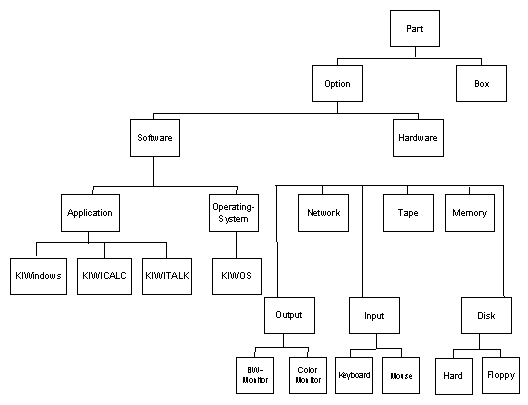
\includegraphics[scale=0.7]{f2-1}
  \caption{Example of a Single Inheritance Hierarchy}
  \label{f:2-1}
\end{figure}

Table~\ref{t:inchar} lists all the characteristics of object classes and
attributes that can be inherited by a subclass. Default
values can be \emph{redefined} by a subclass; the declaration in the
subclass overrides the declaration in the parent class for
that subclass and for all classes inheriting from it.
Attribute structure cannot be redefined; it is a compile-time
error to try to redefine a scalar attribute to be compound,
or vice-versa.
\begin{table}[h]
  \begin{tabularx}{\columnwidth}{Xcl}
    \toprule
    Characteristic              & Can be Redefined?      & Details in section\ldots   \\
    \midrule
    Membership in the parent class    & No          & Object Class Hierarchy \\
    Attribute names             & No          & Attributes   \\
    Attribute structure         & No          & Compound Attributes     \\
    Data type of each attribute & No          & Data Type Declaration    \\
    Default value of each attribute       & Yes         & Default Value \\
    \bottomrule
  \end{tabularx}
  \caption{Inherited Characteristics}
  \label{t:inchar}
\end{table}  

RuleWorks provides an implicit top-level object class called
\verb|$ROOT|. Any object class that you declare without an explicit
\tt{INHERITS-FROM} clause is treated as though you declared the parent
class \verb|$ROOT|. Figure~\ref{f:2-2} shows the implied hierarchy for
the top-level user-declared object classes in the sample program
\tt{KIWI.RUL}.

The specificity of a class is measured by its distance from
\verb|$ROOT| in the inheritance hierarchy. Any top-level user-declared
object class, such as those shown in Figure~\ref{f:2-2} has class specificity
of one. Object classes \tt{SOFTWARE-OPTION} and \tt{HARDWARE-OPTION},
shown in Figure~\ref{f:2-1} have class specificity of three. Object
classes \tt{HD-30} and \tt{HD-200} have class specificity of six.

\begin{figure}[h]
  \centering
  \input f2-2.tex
  \caption{Inheritance from \tt{\$ROOT}}
  \label{f:2-2}
\end{figure}

\section{Working Memory Objects}

A working-memory object (WMO), sometimes called simply an
object, is a collection of attributes each with some value
(one or more atoms, or units of data) that represents a thing
or concept and its associated characteristics. In addition to
attributes with values, each object has a class name, an
identifier, and a time-tag. Figure~\ref{f:2-3} illustrates how
objects are stored in working memory.

\begin{figure}[h]
  \centering
  \input f2-3.tex
  \caption{Conceptual Model of a Working-Memory Object}
  \label{f:2-3}
\end{figure}

\begin{quote}
  \textbf{Note:} The left-to-right order of the attributes shown in
  the figures do not necessarily reflect the actual internal
  representation. In RuleWorks you cannot depend upon the position of
  attributes in a WMO.
\end{quote}

All WMOs inherit two read-only attributes from the built-in
top-level class \verb|$ROOT|: \verb|^$ID| and \verb|^$INSTANCE-OF|. These
attributes store the instance identifier and class name of
the WMO (see Object Identifiers and Class Name)

RuleWorks displays WMOs in the following format:

\begin{quote}
  \verb|#|\it{id} \it{time-tag} \verb|(|\it{class-name}
  \verb|[|\it{rule-name}\verb|]| [\{\ct\it{attribute-name}
  \it{attribute-value}\} \ldots]\verb|)|
\end{quote}

For example:

\begin{quote}
\begin{verbatim}
#297 2529 (PERSON [INIT-DB] ^GIVEN-NAME LARRY ^LAST-NAME KIRK
    ^CHILDREN (COMPOUND ALEXANDER ALICIA ANDREW) ^SPOUSE NINA)
\end{verbatim}
\end{quote}

RuleWorks does not include the names \verb|^$ID| and \verb|^$INSTANCE-OF|
when it displays a WMO, but it does include the values of
these attributes. RuleWorks does not display scalar
attributes whose value is \tt{NIL}, nor compound attributes that
have no elements, unless you have declared a default value
for the attribute (see Default Value Declarations for more on
default values).

\subsubsection*{Object Identifiers}

RuleWorks associates a unique identifier with each object
when it is created. This object identifier has the data type
\tt{INSTANCE-ID}. Unlike the time-tag, which is updated each time
the object is modified, the object identifier is guaranteed
to remain unchanged during the life of the object. Object
identifiers are stored in a built-in, read-only attribute
called \verb|^$ID|. It is an error to attempt to modify \verb|^$ID|.

A variable bound to an \tt{INSTANCE-ID} value is called an \tt{ID}
variable.

\tt{ID} variables can be compared for identity or non-identity,
as in the following rule, but nothing else:

\begin{example}[h]
\begin{quote}
\begin{verbatim}
(rule
  verify-configuration:kiwindows-needs-2-memory-cards-found-one
  ;This rule matches when there is exactly one object of class
  memory
  (active-context ^name verify-configuration)
  (kiwindows)
  (memory ^$id <mem-id>) ; there is one MEMORY
  -(memory ^$id <> <mem-id>) ; but there isn't another one
-->
  (make error ^severity warning ^message |Insufficient memory|)
  (write (crlf) |Caution: KiWindows requires two memory cards,|
         (crlf) | but you have only one memory card.|
         (crlf) | Fixup: adding another memory card to your order.|
         (crlf))
         (make memory))
\end{verbatim}
\end{quote}
\caption{Comparing Object Identifiers}
\end{example}

\subsubsection*{Class Name}

A \emph{class name} is a symbol that identifies the class of which the
object is an instance. Objects that are instances of the same class
always have the same attributes, but the values of the attributes can
be different. The \tt{INSTANCE-ID} and time-tag of each object are
unique to that object.

Figure~\ref{f:2-4} shows seven different objects with the class name
\tt{CONTEXT}. Each of the seven has the same attribute, \verb|^NAME|,
but each has a different value for that attribute.

\begin{figure}[h]
  \centering
  \input f2-4.tex
  \caption{Multiple Objects of One Class}
  \label{f:2-4}
\end{figure}

The class name of an object is stored in a built-in,
read-only attribute named \verb|^$INSTANCE-OF|. You can use this
attribute on the LHS of a rule, but you cannot modify it.

\subsubsection*{Time-Tags}

\emph{Time-tags} are integers that the run-time system uses to
determine recency during conflict resolution. You cannot match or
modify time-tags. The run-time system assigns a unique time-tag to
each object in working memory. The time-tag is automatically updated
whenever the object is modified. Therefore, the object with the
largest time-tag is the most recently created or changed.

\section{Attributes}

An attribute consists of the attribute operator (\verb|^|) followed
by an attribute name that describes a characteristic of the
object class. Attribute names are symbols and are declared in
the \tt{OBJECT-CLASS} declaration.

Attributes can be declared in a parent class or in any
inheriting subclass. For example, all components of the
Kiwi-9200 share some attributes by virtue of being a \tt{PART}.
These attributes (\verb|^PART-NUMBER|, \verb|^NAME|, \verb|^PRICE|, and
\verb|^IS-EXPANDED|) are specified in the \tt{OBJECT-CLASS} declaration
of \tt{PART} and propagated down from \tt{PART} to \tt{OPTION}, to
\tt{HARDWARE-OPTION} and \tt{SOFTWARE-OPTION}, and so on, by
inheritance. The attributes that distinguish hardware from
software are specified in separate \tt{OBJECT-CLASS} declarations.
(See Example~\ref{e:declattr})

\begin{example}[h]
\begin{quote}
\begin{verbatim}
;The OBJECT-CLASS HARDWARE-OPTION. Hardware-options
;have to know whether they take up a slot in the
;CPU box, whether they have been placed in a slot,
;and what slot they are in.

(object-class hardware-option
    (inherits-from option)
    ^takes-slot
    ^is-placed
    ^in-slot)

;The OBJECT-CLASS SOFTWARE-OPTION. All software
;options have a media type as well as the
;other attributes inherited from OPTION and PART.

(object-class software-option
    (inherits-from option)
    ^media-type)
\end{verbatim}
\end{quote}
\caption{Declaring Additional Attributes}
\label{e:declattr}
\end{example}

Suppose you want to specify an object that has the class name
\tt{KIWICALC}, is distributed on a 3.5-inch floppy disk, has part
number S-CA-9200, name KiwiCalc Spreadsheet Software, price {\$}29.95,
and a status flag whose value is \tt{YES}. You can specify this object
as shown in the example.

\begin{example}[h]
\begin{quote}
\begin{verbatim}
(kiwicalc ^media-type FD-35
          ^part-number S-CA-9200
          ^name |KiwiCalc Spreadsheet Software|
          ^price 29.95
          ^is-expanded yes)
\end{verbatim}
You can declare this object class as follows:
\begin{verbatim}
(object-class kiwicalc
    (inherits-from kiwos-application))
\end{verbatim}           
In this example, all the attributes are inherited. For a detailed
description of the \tt{OBJECT-CLASS} declaration, see
Chapter~\ref{c:conditionelements} of this manual.
\end{quote}
\caption{Specifying an Object}
\label{e:specobj}
\end{example}

Attributes are local to an object class and its descendants;
you can use the same attribute name in unrelated object
classes. For example, the attribute \verb|^NAME| is used in both of
the following objects:

\begin{quote}
\begin{verbatim}
(context ^name input-order)
(kiwicalc ^media-type fd-35 ^name kiwicalc)
\end{verbatim}
\end{quote}

\subsubsection{Scalar Attributes}

The value of a scalar attribute is a single atom (see the
section Atoms). For example:

\begin{quote}
\begin{verbatim}
^name |KiwiCalc Spreadsheet Software|
^price 29.95
\end{verbatim}
\end{quote}

The values of these attributes are the symbolic atom
\verb,|KiwiCalc Spreadsheet Software|, and the floating-point atom
29.95. The figure shows how the run-time system stores the
scalar attribute values for a \tt{KIWICALC} object.

\begin{figure}[h]
  \centering
  \input f2-5.tex
  \caption{Storing the Values of Scalar Attributes}
  \label{f:2-5}
\end{figure}

\subsubsection*{Compound Attributes}

A \emph{compound attribute} contains a dynamically-sized, ordered
collection of scalar values. Such a collection is called a
\emph{compound value}. When a compound attribute is bound to a
variable, the variable is called a \emph{compound variable} and has a
compound value. The individual scalar atoms are called \emph{elements}
of the compound value.

Compound values are created (and displayed) with the \tt{COMPOUND}
function. For example:

\begin{quote}
\begin{verbatim}
(compound memory memory keyboard fd-35)
\end{verbatim}
\end{quote}

RuleWorks does not have multilevel lists like LISP; the
result of concatenating the compound value \tt{(COMPOUND A B C)},
the atom \tt{D}, and the compound value \tt{(COMPOUND E F)} is the
compound value \tt{(COMPOUND A B C D E F)}, not the multilevel
list \tt{((A B C) D (E F))}.

Figure~\ref{f:2-6} shows a conceptual model of an object class that
has two compound attributes.

\begin{figure}[h]
  \centering
  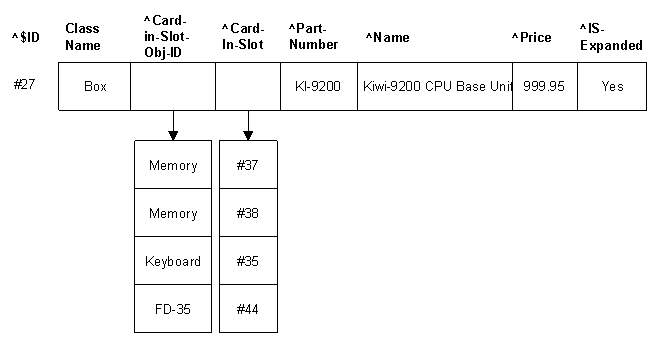
\includegraphics[scale=0.7]{f2-6}
  \caption{Conceptual Model of Compound Attributes}
  \label{f:2-6}
\end{figure}

The object in Figure~\ref{f:2-6} has the class name \tt{BOX}; the scalar
attributes \verb|^PART-NUMBER|, \verb|^NAME|, \verb|^PRICE|, and
\verb|^IS-EXPANDED|; and the compound attributes \verb|^CARD-IN-SLOT|
and \verb|^CARD-IN-SLOT-OBJ-ID|. Note that the left-to-right order of
the attributes in the figure does not necessarily reflect the actual
internal representation of an object. The top-down order of the values
in the compound attributes, however, does match the actual
representation. Compound attributes are indexed starting at 1 (not
0). The first element of \verb|^CARD-IN-SLOT| has the value
\verb|MEMORY|; the fourth and last has the value \verb|FD-35|.

There is no preset limit on the number of atoms allowed in compound
attributes; their size is limited only by memory available. You do not
need to allocate memory for them. The size of a compound value varies
during a program's execution.  See Chapter~\ref{c:conditionelements}
for information on matching compound attributes; see Chapter 4 for
information on creating and changing compound values.

Use the \tt{COMPOUND} keyword in an \tt{OBJECT-CLASS} declaration to
define the name of a compound attribute.
\begin{quote}
\begin{verbatim}
(object-class box
    (inherits-from part)
    ^card-in-slot compound
    ^card-in-slot-obj-id compound)
\end{verbatim}
\end{quote}

The compound attribute declaration is local to the object
class (and its inheriting subclasses), so it is possible for
an attribute name to be compound in one object class and
scalar in another. It is not possible for an attribute to be
compound in the parent class but scalar in a subclass, or
vice-versa.

\subsubsection{Data Type Declarations}

By default, the value of a scalar attribute can have any
valid atomic data type, and the value of a compound attribute
can be a mixture of data types. RuleWorks uses a weak typing
system for attribute values. That is, data type declarations
are not required but if you provide one, RuleWorks enforces
it.

Data types can be added to the \tt{OBJECT-CLASS} declaration after
the attribute name whose type you want to specify as shown in
the following:.

\begin{quote}
  \verb|(object-class| \it{class-name} \{\verb|^|\it{attribute-name}
    [\verb|COMPOUND|] \it{data-type}\} \ldots \verb|)|
\end{quote}

For example:

\begin{quote}
\begin{verbatim}
(object-class person
    ^name symbol
    ^age integer
    ^children compound symbol)
\end{verbatim}
\end{quote}

Table~\ref{t:2-2} shows the symbols that can be used in data type
declarations for attributes.

\begin{table}[h]
  \centering
  \begin{tabular}{lll}
    \toprule
    Data Type & Description & Default value \\
    \midrule
    \tt{INTEGER}     & Integer number        & \tt{0} \\
    \tt{FLOAT}       & Floating point number & \tt{0.0} \\
    \tt{NUMBER}      & Either kind of number & \tt{0} \\
    \tt{SYMBOL}      & Symbolic atom         & \tt{NIL} \\
    \tt{INSTANCE-ID} & Object identifier     & \verb|#0| \\
    \tt{OPAQUE}      & Virtual address       & \verb|%x0| \\
    \tt{ANY}         & Any of the above      & \tt{NIL} \\  
    \bottomrule
  \end{tabular}
  \caption{Data Types for Attributes}
  \label{t:2-2}
\end{table}

RuleWorks does not perform automatic coercion on values
assigned to typed attributes, not even between integers and
floats. To ensure that a value has the correct type, use one
of the built-in coercion functions: \tt{FLOAT}, \tt{INTEGER}, or
\tt{SYMBOL}.

\subsubsection{Default Value Declarations}

When you create an object, you do not need to specify a value
for each attribute. RuleWorks supplies a default value for
attributes whose values were not specified. You can specify
the default value for each attribute, or use RuleWorks's
default.

If an attribute does not have a data-type declaration, the default
value is the \tt{NIL} for scalar attributes and the empty list
(\tt{(COMPOUND)}) for compound attributes. If an attribute has a data
type declaration but does not have default value declaration, its
default value depends on its data type (see Table~\ref{t:2-2}).

You specify a default value for an attribute with the \tt{DEFAULT}
keyword in the \tt{OBJECT-CLASS} declaration. The following
example shows the declaration of the \tt{PART} class from the
sample configuration program.

\begin{quote}
\begin{verbatim}
(object-class part
    ^part-number
    ^name
    ^price 
    ^is-expanded (default no))
\end{verbatim}
\end{quote}

When any object that inherits from class \tt{PART} is made, and no
new value for the \verb|^IS-EXPANDED| attribute is specified, the
value of that attribute is \tt{NO}.

For a compound attribute, the specified default value is
itself a compound value that will be used as the initial
contents of the attribute, if none is specified in the \tt{MAKE}
action. The following example declares an initial value for
the hypothetical compound attribute \verb|^TASKS|:

\begin{quote}
\begin{verbatim}
(object-class agenda
    ^tasks compound symbol
       (default (compound input-order
                          convert-to-parts
                          verify-configuration
                          expand-part-skeletons
                          choose-slots
                          modify-software-media
                          output-new-order)))
\end{verbatim}
\end{quote}

\subsubsection{Fill Value Declarations}

You can modify a compound attribute by specifying a new value for any
element. Thus, it is possible to modify a compound attribute``beyond''
the last assigned element. The question arises, what value do elements
between the former end and the new end of the compound now have? To
answer this question, RuleWorks allows you to declare a \emph{fill},
or placeholder, value for the compound attribute.

RuleWorks' default fill value depends on the data type of the compound
attribute, if any. You specify a different fill value in the
\tt{OBJECT-CLASS} declaration, after the \tt{COMPOUND} keyword. For
example, consider the declaration shown below:

\begin{quote}
\begin{verbatim}
(object-class agenda
    ^tasks compound
       (default (compound input verify output))
       (fill no-op))
\end{verbatim}
\end{quote}

When an \tt{AGENDA} object is made, the default value of its
\verb|^TASKS| attribute is \tt{(COMPOUND INPUT VERIFY
  OUTPUT)}. Suppose the following \tt{MODIFY} action is executed:

\begin{quote}
\begin{verbatim}
(modify <my-agenda> ^tasks[5] clean-up)
\end{verbatim}
\end{quote}

The value of \verb|^TASKS| is now \tt{(COMPOUND INPUT VERIFY OUTPUT
  NO-OP CLEAN-UP)}.

Default Value Declarations explains how to specify a default value for
the entire compound attribute.

\section{Value Expressions}

In RuleWorks an attribute value can be set by using a constant, a
variable, an arithmetic expression, a function call, or an expression
that contains any of these things.

\subsection{Atoms}

The smallest unit of data in a RuleWorks program is called an
atom. Atoms must be one of the data types listed in Table~\ref{t:2-2}.

\subsubsection{Symbolic and Quoted Atoms}

A symbolic atom is one that does not have a numeric value. A symbol
consists of from 0 to 256 printable ASCII characters on a single
line. For example:

\begin{quote}
\begin{verbatim}
c
PLANT
?-c
10-14
\end{verbatim}
\end{quote}

RuleWorks supports the eight-bit DEC Multinational Character
Set. Table~\ref{t:2-3} lists the characters that cannot be used in
unquoted RuleWorks symbols.

\begin{table}[h]
  \centering
  \begin{tabular}{ll}
    \toprule
    Character & Description \\
    \midrule
    Parenthesis (\verb|()|) & Enclose rules, actions, and so on. \\
    Braces (\verb|{}|) & Indicate conjunctions. \\
    Brackets (\verb|[]|) & Index compound attributes. \\
    Caret (\verb|^|) & The attribute operator. \\
    Semicolon (\verb|;|) & The comment character. \\
    Vertical bar (\verb,|,) & The quote character. \\
    Pound sign (\verb|#|)  & Indicates an instance identifier. \\
    Percent sign (\verb|%|) & Indicates an opaque address. \\
    White space & Tokens (space, tab, line feed, form feed, vertical tab). \\
    Ampersand (\verb|&|) & Reserved for future use.  \\
    Double-quote (\verb|"|) & Reserved for future use. \\
    Tilde (\verb|~|) & Reserved for future use. \\
    \bottomrule
  \end{tabular}
  \caption{Special Characters}
  \label{t:2-3}
\end{table}

\begin{quote}
  \textbf{Note:} RuleWorks does not support null characters in any
  symbol, quoted or not.
\end{quote}

To include special characters or white space in an atom, quote the
atom by enclosing it in vertical bars (\verb,||,). The text between
the two vertical bars is considered to be one symbolic atom. For
example, the compiler and run-time system recognize
\verb|THIS IS AN ATOM;| \verb|THIS IS NOT| to be four symbolic atoms followed
by a comment, which they ignore. However, they recognize
\verb,|THIS IS AN ATOM;, \verb,THIS IS NOT|, to be a single symbolic
atom.

Quoted atoms are symbolic atoms; therefore, \verb,|1.2|, is a symbol,
not a floating-point number, and arithmetic operations cannot be
performed on it. The opening and closing vertical bars, which can
enclose as many as 256 characters, must appear on the same line in the
code. The empty symbol are vertical bars enclosing nothing
(\verb,||,).

To quote a vertical bar itself, double it. For example:

\begin{quote}
\begin{verbatim}
|This is a vertical bar - ||.|
\end{verbatim}
\end{quote}

When this atom is displayed or printed, it includes only one
vertical bar:

\begin{quote}
\begin{verbatim}
This is a vertical bar - |.
\end{verbatim}
\end{quote}

When reading unquoted symbols, RuleWorks automatically turns lowercase
characters into uppercase. An unquoted symbol printed by RuleWorks may
appear to be different from the symbol read by RuleWorks. If you want
the print form to be the same as the read form, you must use quoted
symbols. The following table shows the read and print forms of several
atoms:

\begin{center}
  \begin{tabular}{lll}
    \toprule
    Read Form & Print Form & Data Type \\
    \midrule
    \verb,A, &  \verb,A, & \tt{SYMBOL} \\
    \verb,a,        & \verb,A,          & \tt{SYMBOL} \\
    \verb,|a|,       & \verb,a,          & \tt{SYMBOL} \\
    \verb,|a b|,     & \verb,a b,        & one \tt{SYMBOL} \\
    \verb,a b,       & \verb,A B,        & two \tt{SYMBOL}s \\
    \verb,|A B|,     & \verb,A B,        & one \tt{SYMBOL} \\
  \bottomrule
  \end{tabular}
\end{center}

All atoms that are not symbols have read forms that are identical to
their print forms.

\subsubsection{Integer Atoms}

Integer atoms consist of the following:

\begin{itemize}
\item An optional plus or minus sign
\item One or more decimal digits
\item An optional decimal point
\end{itemize}

The following are examples of integer atoms:

\begin{quote}
\begin{verbatim}
0
25.
-14
-5.
\end{verbatim}
\end{quote}

Integer atoms can represent the same range of values as a ``long'' in
the C language. On Digital UNIX for Alpha, integers are 64 bits. That
is, the valid range for integer atoms is $-2^{63}$ to $2^{63}- 1$. On
all other systems, integers are 32 bits or $-2^{31}$ to $2^{31}-1$.

\subsubsection{Floating-Point Atoms}

A floating-point atom is composed of the following:

\begin{itemize}
\item An optional plus or minus sign
\item Zero or more decimal digits
\item A decimal point
\item Either one or both of these:
  \begin{itemize}
  \item One or more decimal digits after the decimal point
  \item An optional exponent
  \end{itemize}
\end{itemize}

An exponent consists of the letter ``E'' followed by a signed
or unsigned integer and represents a power of 10 by which a
preceding number is to be multiplied. For example, E-8
represents the value 10 raised to the power -8.

\begin{note}
  A floating-point atom must include a decimal point followed by a
  digit or an exponent, or both.
\end{note}

The following are examples of floating-point atoms:

\begin{quote}
\begin{verbatim}
0.0
.25
10.05e-14
-5.e10
\end{verbatim}
\end{quote}

Floating-point numbers are stored in double-precision and can
represent the same range of values as a ``double'' in the C
language. (On VAX systems, this is \verb|D_float data|; see the
\emph{VAX Architecture Handbook}. On Alpha systems, this is
\verb|G_float| data; see the \emph{Alpha Architecture Handbook}.)

\subsubsection{Instance Identifier Atoms}

Values of type \tt{INSTANCE-ID} are used to identify objects.
RuleWorks displays (and you type) an \tt{INSTANCE-ID} atom as a number
sign (\verb|#|) followed by an integer.

\begin{quote}
\begin{verbatim}
#1
#7955
\end{verbatim}
\end{quote}

\begin{note}
  \tt{INSTANCE-ID}s are not integers. Arithmetic operations cannot be
  applied to values of type \tt{INSTANCE-ID}, and they cannot be
  compared except for identity or nonidentity.
\end{note}

More information on variables bound to atoms of type \tt{INSTANCE-ID}
is found in Chapter~\ref{c:conditionelements}.

\subsubsection{Virtual Address Atoms}

Values of type \tt{OPAQUE} store addresses of functions or
external data structures. An \tt{OPAQUE} value is an ``atomic
address'' or in C terms, a ``void *''.

The print form of an \tt{OPAQUE} atom is a percent sign and an \verb|x|
(\verb|%x|) followed by a string of hexadecimal digits. The size of
\tt{OPAQUE} atoms depends on the machine architecture you are
using. Note that \tt{OPAQUE} may or may not be the same size as
the \tt{INTEGER} data type.

There is no way in RuleWorks directly to create a constant of
type \tt{OPAQUE}, except for the null pointer which is a RuleWorks
constant. For example:

\begin{quote}
\begin{verbatim}
%x0 ; the null pointer
\end{verbatim}
\end{quote}

An \tt{OPAQUE} constant can be passed into RuleWorks from an
external routine, or as an input argument to an entry block,
and then passed out or returned.

\begin{note}
  \tt{OPAQUE} atoms are not numbers. Arithmetic operations cannot be
  applied to values of type \tt{OPAQUE}, and they cannot be compared
  except for identity or nonidentity.
\end{note}

\subsection{Variables}

A variable is any unquoted symbol enclosed in angle brackets
(\verb|<>|). An example is \verb|<PRICE>|.

\begin{note}
  In RuleWorks, the symbols \verb|<=>| and \verb|<->| represent the
  same-type and different-type operators. They cannot be used as
  variables.
\end{note}

You can use a variable as an argument to an action if the variable is
bound to a value. A variable can be bound to a value in a condition
element or in a \tt{BIND} action.

The following \tt{WRITE} action has two arguments: a quoted symbolic
atom and a bound variable.

\begin{quote}
\begin{verbatim}
(write |The value found was:| <x>)
\end{verbatim}
\end{quote}

\subsection{Arithmetic Expressions}

Arithmetic expressions can be used anywhere a numeric constant may be
used. An arithmetic expression can contain numbers, variables bound to
numbers, functions which return numbers, and arithmetic operators. The
expression must be enclosed in parentheses, except when indexing into
a compound value. For example:

\begin{quote}
\begin{verbatim}
^price = (<item-1> + <item-2>) ; add two bound variables
^card-in-slot[<n> + 1] memory ; add a variable and a constant
\end{verbatim}
\end{quote}

The valid operators are:

\begin{center}
  \begin{tabular}{ll}
    \toprule
    Operator & Description    \\
    \midrule
    \verb|+|  & Addition       \\
    \verb|-|  & Subtraction    \\
    \verb|*|  & Multiplication \\
    \verb|/|  & Division       \\
    \verb|\|  & Modulus        \\
    \bottomrule
  \end{tabular}
\end{center}

If an expression contains both integers and floating-point numbers,
the result is a floating-point number. If an expression contains
integers only, the result is an integer (by truncation). For example,
7.0 (float) divided by 4 (integer) is 1.75 (float), but 7 (integer)
divided by 4 (integer) is 1 (integer).

\begin{note}
Use the modulus operator only with integer operands.
\end{note}

Use infix notation in RuleWorks arithmetic expressions, that is, place
operators between operands. Separate each operator and operand with a
space. Surround the entire expression with parentheses. For example:

\begin{quote}
\begin{verbatim}
(2 + <X>)
\end{verbatim}
\end{quote}

Spaces are not required around any of the special characters in the
first five rows of the table.

Expressions are evaluated from left to right. Precedence of operators
follows the normal conventions:

\begin{quote}
\verb|-|  ; unary negation, highest precedence

\verb|*| \verb|/| \verb|\| ; multiplication, division, and modulus

\verb|+| \verb|-|  ; addition and subtraction, lowest precedence
\end{quote}

For example, the following expression evaluates to 12, not 20:

\begin{quote}
\begin{verbatim}
(2 + 2 * 5)
\end{verbatim}
\end{quote}

To override the normal precedence, use more parentheses. The following
expression does evaluate to 20:

\begin{quote}
\begin{verbatim}
((2 + 2)* 5)
\end{verbatim}
\end{quote}

Consider the following rule:
\begin{quote}
\begin{verbatim}
(rule choose-slots:place-memory
    (active-context ^name choose-slots)
    (box ^$ID <the-box> ^card-in-slot { [=] <len> [<] 6 })
    (memory ^$ID <the-mem> ^is-placed nil ^takes-slot yes)
  -->
    (modify <the-box>
        ^card-in-slot [ ( <len> + 1 ) ] memory
        ^card-in-slot-obj-id [ ( <len> + 1 ) ] <the-mem>)
    (modify <the-mem> ^is-placed yes ^in-slot ( <len> + 1 )))
\end{verbatim}
\end{quote}
    
The \tt{MODIFY} actions in this rule use numeric expressions for
the index into a compound attribute and for the value of a
scalar attribute.

\begin{note}
  RuleWorks does not have complex mathematical functions built in. For
  example, RuleWorks has no \tt{ARC-COSINE} function.  For such
  complex mathematical functions, a RuleWorks program can call
  external routines written in other languages that are optimized for
  algorithmic coding.
\end{note}

\subsection{Function Calls}

The format for specifying a function call is:

\begin{quote}
  \verb|(|\it{function-name} \it{argument-1} \it{argument-2} \ldots\verb|)|
\end{quote}

Use the same format whether the function is built-in or user-defined
(as an external function or an entry block that returns a value).

\begin{note}
  If a function requires no arguments, you must still enclose the
  function name in parentheses.
\end{note}

You can represent a value with a call to a built-in RuleWorks
function. Consider the following \tt{MAKE} action:

\begin{quote}
\begin{verbatim}
(make input-thing ^item (accept-atom infil))
\end{verbatim}
\end{quote}

First, the run-time system evaluates the call to the \tt{ACCEPT-ATOM}
function. The \tt{MAKE} action then stores the value returned by the
\tt{ACCEPT-ATOM} function in the \verb|^ITEM| attribute of the
\tt{INPUT-THING} object it creates.

You can also represent a value with a call to a user-defined function,
written in RuleWorks or some other language. In either case, you must
declare the function before you call it. The following \tt{BIND}
action calls the external function \verb|SQUARE-ROOT|:

\begin{quote}
\begin{verbatim}
(bind <std-deviation> (square-root <variance>))
\end{verbatim}
\end{quote}

%%% Local Variables:
%%% mode: latex
%%% TeX-master: "rwug"
%%% End:

\chapter{Rules' Left-Hand Sides: Condition Elements}
\label{c:conditionelements}

The left-hand side (LHS) is the ``if'' part of a rule. It specifies
the conditions in working memory that must be true before the rule can
fire. The LHS is composed of \emph{condition elements}, each of which
can match objects of a particular class (and its subclasses, if
any). Condition elements can also test for particular attribute
values, and bind variables to those values. The variables can be used
only later in the same rule.

Condition elements (CEs) must be enclosed in parentheses.  CEs can be
positive, stating that certain conditions are true; or negative,
stating that certain conditions are false. A negative CE has a minus
sign (\verb|-|) before its opening parenthesis. The first CE on an LHS
must be positive.

RuleWorks performs an implicit conjunction (a logical AND operation)
on all the CEs on an LHS. A rule is eligible to fire when there are
objects that match all of its positive CEs, and there are no objects
that match any of its negative CEs. It is also possible to specify a
disjunction (a logical OR operation) of CEs.

\section{Matching the Object Class}

The first item in each CE must be the name of a declared
object class. The class name is the only required item. In
the example below, the CE (start) matches the object made
in the \tt{ON-ENTRY} statement.

\begin{quote}
\begin{verbatim}
(entry-block main)
    (object-class start)
    (on-entry (make start))
    (rule say-hello
        (start)
      -->
        (write |Hello, world!|))
(end-block main)
\end{verbatim}
\end{quote}

Example~\ref{e:obclasdecl} hows some \tt{OBJECT-CLASS} declarations
from the sample configuration program, \tt{KIWI.RUL}.

\begin{example}[h]
\begin{quote}
\begin{verbatim}
(object-class part
    ^part-number
    ^name
    ^price
    ^is-expanded)

(object-class option
    (inherits-from part))

(object-class hardware-option
    (inherits-from option)
    ^takes-slot
    ^in-slot
    ^is-placed)

(object-class memory
    (inherits-from hardware-option))
\end{verbatim}
\end{quote}
\caption{Sample \tt{OBJECT-CLASS} Declarations}
\label{e:obclasdecl}
\end{example}

When the class name in a CE is a parent class, objects of any of its
inheriting subclasses can also match the CE.  Given the
\tt{OBJECT-CLASS} declarations in Example~\ref{e:obclasdecl},
Table~\ref{t:matchingobclass} shows which objects match each
class. For example, an object of class \tt{MEMORY} can match a CE that
specifies any of the declared class names shown, but only an object of
class \tt{PART} can match a CE that specifies the class name
\tt{PART}.

\begin{table}[h]
  \centering
  \begin{tabular}{lllll}
    \toprule
    An Object of Class & \multicolumn{4}{l}{Matches a Condition Element of  Class} \\
    \midrule
    & \tt{PART} & \tt{OPTION} & \tt{HARDWARE-OPTION} & \tt{MEMORY} \\
    \midrule
    \tt{PART}               & Yes  & No     & No       & No  \\
    \tt{OPTION}             & Yes  & Yes    & No       & No  \\
    \tt{HARDWARE-OPTION}    & Yes  & Yes    & Yes      & No  \\
    \tt{MEMORY}             & Yes  & Yes    & Yes      & Yes  \\
    \bottomrule
  \end{tabular}
  \caption{Matching Object Classes}
  \label{t:matchingobclass}
\end{table}

An object of any visible user-declared class matches a CE that
specifies the built-in top-level class \verb|$ROOT|.

Rules can refer only to classes that are visible to the entry block or
rule block that contains them. See Chapter~\ref{c:program} for
information on making object classes visible to more than one block.

Rules can refer to a parent class or to a specific subclass. In
the following example, the rule
\tt{VERIFY-CONF:APPLICATION-NEEDS-KIWOS} applies to any one
of the software applications: \tt{KiWindows}, \tt{KiwiCalc}, or
\tt{KiwiTalk}. Conversely, rule
\tt{VERIFY-CONF:KIWITALK-NEEDS-NETWORK} applies only to
\tt{KiwiTalk}, not to \tt{KiWindows} or \tt{KiwiCalc}.

\begin{quote}
\begin{verbatim}
(rule verify-conf:application-needs-kiwos
  (active-context ^name verify-conf)
  (kiwos-application ^$instance-of <applic>)
  - (kiwos)
-->
  (make error ^severity warning ^message |Missing operating system|)
  (write (crlf) |Caution: to run application:| <applic>
     (crlf) |you need to have KIWOS, but you don't have KIWOS.|
     (crlf) |Fixup: adding KIWOS to your order.|
     (crlf))
  (make kiwos))

(rule verify-conf:kiwitalk-needs-network
  (active-context ^name verify-conf)
  (kiwitalk)
  -(network-interface)
-->
  (make error ^severity warning ^message |Missing network interface|)
  (write (crlf) |Caution: you ordered KiwiTalk, but don't have|
     (crlf) |the network interface hardware to use KiwiTalk.|
     (crlf) |Fixup: adding a network interface to your order.|
     (crlf))

  (make network-interface))
\end{verbatim}
\end{quote}

\begin{note}
  Any attribute accessed in a rule must either be declared in the
  class itself or be inherited from a parent class. RuleWorks
  generates a compile-time error if this requirement is not followed.
\end{note}

\section{Writing Attribute-Value Tests}

After the required class name, a CE can contain any number of
attribute-value tests. These are the patterns that objects in working
memory must match in order for the rule to fire. Attribute-value tests
consist of an attribute name, a predicate, and a value. You can make
combinations of tests on a single attribute by using conjunctions and
disjunctions, which are similar to AND and OR operators.

The number of attribute-value tests on the LHS determines the test
specificity of a rule. Test specificity is one of the principles used
during conflict resolution (see Test Specificity).

\subsection{Attribute Names}

The attribute name in an attribute-value test must be one
of the following constructs:
\begin{itemize}
\item the name of an attribute declared in the CE's object class (or
  declared in an ancestor of that object class)
\item the name of a built-in attribute
\end{itemize}
The attribute operator (\verb|^|) must precede the attribute name.

Given the declarations in the example above, the following are valid
CEs:

\begin{quote}
\begin{verbatim}
(part ^part-number KI-9200)
(option ^part-number KI-9200)
(hardware-option ^part-number KI-9200 ^takes-slot yes)
(memory ^part-number KI-9200 ^takes-slot yes)
\end{verbatim}
\end{quote}

The following CEs are not valid because the attributes
have not been declared for the object classes:

\begin{quote}
\begin{verbatim}
(part ^takes-slot no)
(option ^is-placed yes)
\end{verbatim}
\end{quote}

The built-in attribute names are \verb|^$INSTANCE-OF| (see
Matching the Exact Class and Matching the Instance
Identifier).

\subsubsection*{Matching the Exact Class}

If you want to match, or bind a variable to, the exact subclass of
which an object is an instance, you can use the built-in, read-only
attribute
\verb|^$INSTANCE-OF|. In the following code fragment, the second CE
binds the value of the \verb|^$INSTANCE-OF| attribute to the variable
\verb|<OPTION>|. This variable is then used in the \verb|MODIFY|
action.

\begin{quote}
\begin{verbatim}
...
(box ^$id <the-box> ^card-in-slot {[=] <len> [<] 8})
(hardware-option ^$id <the-option> ^$instance-of <option>
  ^takes-slot yes ^is-placed no )
-->
(modify <the-box>
  ^card-in-slot [(<len> + 1)] <option>
  ^card-in-slot-obj-id [(<len> + 1)] <the-option>)
...
\end{verbatim}
\end{quote}
In this example, \verb|<OPTION>| might be bound to the symbol
\verb|MEMORY|.

\subsubsection{Matching the Instance Identifier}

The built-in, read-only attribute
\verb|^$ID| stores the \tt{INSTANCE-ID} value of the object. If you
want to copy, modify, or remove an object on the RHS, you usually
first bind a variable to its identifier on the LHS. Such a variable is
called a \verb|$ID| variable.
\verb|$ID| variables give you a handle on the object that matched a
CE. \verb|$ID| variables in RuleWorks are similar to element variables
in previous versions of OPS.

You can use variables bound to values of type \tt{INSTANCE-ID} as
pointers to maintain links between objects. Example~\ref{e:3-5} shows a
RuleWorks program that uses such pointers to build a doubly linked
list of objects. Note that the variables \verb|<FIRST-DATA>| and
\verb|<LAST-DATA>| are
\verb|$ID| variables, but the variable \verb|<PREVIOUS-DATA>| is
not. Variable \verb|<NEW-DATA>|, which is bound on the right-hand
side, is not a \verb|$ID| variable. Variables \verb|<PREVIOUS-DATA>|
and \verb|<NEW-DATA>| cannot be used in \tt{MODIFY} actions as
variables \verb|<FIRST-DATA>| and \verb|<LAST-DATA>| are.

\begin{example}[!h]
\renewcommand{\baselinestretch}{0.9}\normalsize
\begin{quote}
\begin{verbatim}
(entry-block pointer-demo)
  (object-class data
      ^previous ; pointer to preceding datum
      ^next ; pointer to following datum
      ^value) ; actual datum

  (object-class pointer
      ^max-length ; desired length of list
      ^list compound) ; pointers to all DATA objects

  (on-entry
      (watch all)
      (make pointer ^max-length 7) ; arbitrary choice
      (make data ^previous nil ^next nil)) ; start with null pointers

  (rule init-list
      ; Initialize the list by making a DATA object with  
      ; pointers to itself
      (pointer ^$id <the-pointer>)
      (data ^$id <the-data> ^previous nil ^next nil)
    -->
      (modify <the-data> ^previous <the-data> ^next <the-data> ^value 1)
      (modify <the-pointer> ^list (compound <the-data>)))

  (rule make-list
      ; Make a new datum and add it to the list
      (pointer ^$id <the-pointer> ^max-length <max>
               ^list {list [<] <max>} ; length of list is less than <MAX>
               ^list[1] <first-data> ; bind ID of first DATA
               ^list[$last] <last-data>)  ; bind ID of last DATA
      (data ^$id <first-data> ; test ID of first DATA
            ^previous <previous-data>) ; bind backward ptr of first item
      (data ^$id <last-data> ; test ID of last DATA
            ^value <val> ; bind value of last item
            ^next <the-data>) ; bind forward ptr of last item
    -->
      (bind <new-data> ; bind a pointer to a MAKE action
          (make data ^previous <last-data> ^next <first-data> 
                     ^value (<val> + 1)))
      (modify <first-data> ^previous <new-data>)
      ; reset pointers to new item
      (modify <last-data> ^next <new-data>)
      (modify <the-pointer> ^list (compound list
      <new-data>)))
(end-block pointer-demo)
\end{verbatim}
\end{quote}
\caption{Using \ct\tt{ID} Variables as Pointers}
\label{e:3-5}
\end{example}

\subsubsection*{Using a Bound Variable to Select an Attribute}

You can use a bound variable to select an attribute on both the LHS
and the RHS. This is useful if a program is treating object data as a
look-up table.

RuleWorks allows a variable-selected attribute to be matched against;
the variable selecting the attribute must be bound before the match
reference is made, and the value must be the name of an attribute in
that object class (see Example~\ref{e:3-6}). RuleWorks issues a run-time
warning if the attribute binding does not exist in the specified
object class.

\begin{example}[h]
\begin{quote}
\begin{verbatim}
(object-class person
    ^name
    ^age
    ^phone_number
    ^address)

(object-class seek_slot ^slot_to_find)

(make person
    ^name |Joe Bloggs|
    ^phone_number 01292-474382
    ^address |17 Anderson Crescent|)

(make person
    ^name |John Doe|
    ^phone_number 0141-887-2456
    ^address |56 Alloway Drive|)

(make seek_slot
    ^slot_to_find phone_number
    ^name Dorothy)

(rule find_arbitrary_slot_datum_given_name
    (seek_slot ^slot_to_find <slot> ^name <person_name>)
    (person ^name <person_name> ^<slot> <datum>)
  -->
    (write (crlf) |Person| <name> |slot| <slot> 
        |has value| <datum>))
\end{verbatim}
\end{quote}
\caption{Variable Selection of Attributes Variable Selection of Attributes}
\label{e:3-6}
\end{example}

\section{Predicates}

The test part of an attribute-value test is a predicate that specifies
the comparison to be performed (equal to, greater than, and so on)
between the atom or atoms in the attribute and the scalar or compound
value in the CE.

Every value specified in a condition element is preceded by a
predicate, either implicitly or explicitly. Values that you specify
without a predicate are implicitly preceded by the identity predicate
(see Identity, Equality, and Similarity Predicates)

\subsubsection*{Predicates and Data Types}

Table~\ref{t:3-2} shows the match predicates of RuleWorks, with the
types of attributes and values to which they can be applied. The
values referred to in the third column of Table~\ref{t:3-2} can be constants,
variables, or other expressions.

While matching condition elements to working memory, RuleWorks
performs automatic data type coercion for ``reasonable''
attribute-value tests only. Table~\ref{t:3-2} also shows which data types are
reasonable for each match predicate. All other mixed-type comparisons
yield ``no match.'' ``No match'' is not an error condition; it merely
means that the query ``A relation B'' will fail, no matter which
relation was requested (greater than, less than, equal to, and so
on). For example, the following test, which will never match, produces
a warning message at compile time, and no message or error condition
at run time:
\begin{quote}
\begin{verbatim}
^$ID < x
\end{verbatim}
\end{quote}

\begin{table}[!h]
  \begin{tabularx}{\columnwidth}{lllX}
    \toprule
    Attribute Domain & Predicate & Value Domain & Test \\
    \midrule
    ANY & \verb|==| & ANY & Identity: Same type as and equal to  (This predicate is optional in  LHS attribute-value tests. It is required in RHS relational expressions.) \\
    ANY & \verb|<>| & ANY & Nonidentity; converse of identity \\
    ANY & \verb|=| & ANY & Equality: Identical or equivalent numbers; identical symbols except for case; identical values of all other data types \\
    ANY & \verb|-=| & ANY & Inequality; converse of equality \\
    ANY & \verb|~=| & ANY & Similarity: Equal or phonetically similar symbols; equal or approximately equal numbers; identical values of all other data types \\
    ANY & \verb|-~=| & ANY & Dissimilarity; converse of similarity \\
    NUMBER & \verb|>| & NUMBER & Greater than \\
    SYMBOL & \verb|>| & SYMBOL & Lexicographically after \\
    ANY & \verb|>=| & ANY &  Greater than or equal numbers; lexicographically after or equal symbols; identical values for all other data types \\
    NUMBER & \verb|<| & NUMBER & Less than \\
    SYMBOL & \verb|<| & SYMBOL & Lexicographically before \\
    ANY & \verb|<=| & ANY & Less than or equal numbers; lexicographically before or equal symbols; identical values for all other data types \\
    ANY & \verb|<=>| & ANY &  Same type \\
    ATOM & \verb|[+]| & COMPOUND & Containment; atom is contained within the compound \\
    ATOM & \verb|[-]| & COMPOUND & Non-containment; converse of containment \\
    COMPOUND & \verb|[+]| & ATOM & Containment; compound contains atom \\
    COMPOUND & \verb|[-]| & ATOM & Non-containment; converse of containment \\
    COMPOUND & \verb|[=]| & INTEGER & Length equal \\
    COMPOUND & \verb|[<>]| & INTEGER & Length not equal \\
    COMPOUND & \verb|[>]| & INTEGER & Length greater \\
    COMPOUND & \verb|[>=]| & INTEGER & Length greater than or equal \\
    COMPOUND & \verb|[<]| & INTEGER & Length less than \\
    COMPOUND & \verb|[<=]| & INTEGER & Length less than or equal \\
    \bottomrule
  \end{tabularx}
\begin{quote}
  * Scalar predicates are those that are valid only for scalar
  attributes. The exceptions are identity and nonidentity (== and <>),
  which are also valid for comparing a compound attribute to a
  compound value.  Compound predicates are those that are valid for
  compound attributes.
\end{quote}
\caption{RuleWorks Match Predicates*}
\label{t:3-2}
\end{table}


For example, the seventh row in Table~\ref{t:3-2} states that any
\tt{NUMBER}, either \tt{FLOAT} or \tt{INTEGER}, can reasonably be
tested for being greater than any other NUMBER. Thus, assuming the
value of \verb|^LIST-PRICE| is the \verb|FLOAT| 29.95, the following
test returns \verb|TRUE|:
\begin{quote}
\begin{verbatim}
^list-price > 20
\end{verbatim}
\end{quote}
The same row also states that the greater-than predicate can be
applied to two symbols. For example, the following test is valid, and
the symbols are compared according to the lexicographic collating
sequence for the target platform (the operating system and hardware
where the executable image will run). Assume that \verb|^ANIMAL| is
bound to the symbol \tt{AARDVARK}, and the following test produces a
match:
\begin{quote}
\begin{verbatim}
^animal < zebra
\end{verbatim}
\end{quote}

A mixed type comparison such as the following generates a compile-time
warning and fails to match at run time:
\begin{quote}
\begin{verbatim}
^$ID < 42
\end{verbatim}
\end{quote}

\subsubsection*{Identity, Equality, and Similarity Predicates}

The identity predicate tests that values are of the same data type and
also equivalent to each other. It executes faster than the equality
predicate, which ignores data type and tests only for equivalent
value. Table~\ref{t:3-3} compares results of using the identity, equality, and
similarity predicates on a \tt{FLOAT} of unequal value, a \tt{FLOAT}
of equal value, and an \tt{INTEGER} of equal value.

\begin{table}[h]
  \centering
  \begin{tabular}{lllll}
    \toprule
    & & \multicolumn{3}{l}{Match if \ct\tt{X} Attribute is \ldots} \\
    \midrule
    Predicate & Example & 11.9 & 12.0 & 12 \\
    \midrule
    Identity & \verb|^x 12| & No & No & Yes \\
    Equality & \verb|^x = 12| & No & Yes & Yes \\
    Similarity & \verb|^x ~= 12| & Yes & Yes & Yes \\
    \bottomrule
  \end{tabular}
  \caption{Identity, Equality, and Similarity Predicates}
  \label{t:3-3}
\end{table}

The identity and nonidentity (\verb|<>|) predicates are the only ones
that can be applied when the attribute and the value are either both
scalar or both compound.

The identity and length-equal predicates are the only ones that can
precede the first occurrence of a variable, because they can be used
to bind a variable to the value of an attribute or to the length of a
compound attribute. The first appearance of a variable on an LHS is
where it is bound to a value. The identity predicate is the only one
that can precede a disjunction of values (see Disjunctions of Values).

\subsection{Specifying Values}

Chapter~\ref{c:workingmem} covers the general rules for specifying
values in RuleWorks. This section explains the restrictions on
constants, variables, and function calls in value expressions on the
LHS.

\subsubsection{Constants}

Constants can be symbols, integers, or floating-point numbers. There
are also two special constants: the instance identifier \verb|#0|,
which never refers to an actual WMO; and the opaque value \verb|%x0|,
which corresponds to the
null pointer provided by most other programming languages.

You cannot use any other \tt{INSTANCE-ID} or \tt{OPAQUE} constant in
source code; use them only in the command interpreter.

\subsubsection{Variables}

The first time a variable appears on an LHS, the variable is bound to
the attribute value in the object that matches the CE. All subsequent
occurrences of that variable in that rule represent the same
value. For example, suppose the LHS of a rule contains the following
CEs:
\begin{quote}
\begin{verbatim}
(memory ^price <price>) ; variable <price> is bound here
(disk ^price > <price>) ; variable <price> is tested here
\end{verbatim}
\end{quote}

If the run-time system finds a match for the first CE, the system
binds the variable \verb|<PRICE>| to the value stored in the
\verb|^PRICE| attribute of the object of class \tt{MEMORY} that
matches the CE. Suppose the variable \verb|<PRICE>| is bound to atom
129.95. Then the second CE is matched by an object of class \tt{DISK}
whose \verb|^PRICE| attribute has a value greater than 129.95.

\subsubsection{Function Calls}

You can use certain built-in or user-defined functions to specify a
value in an attribute-value test. Functions used on the LHS must not
change any objects in working memory and must always return the same
result when called with the same arguments.

The built-in RuleWorks functions that can be used on the LHS are
listed in Table~\ref{t:3-4} and Table~\ref{t:3-5}.

\begin{table}[h]
  \centering
  \begin{tabular}{ll}
    \toprule
    Name & Description \\
    \midrule
    \tt{FLOAT} &  Converts a numeric value into afloating-point number. \\
    \tt{INTEGER} &  Converts a numeric value into an integer. \\
    \tt{SYMBOL} & Converts any atom into a symbol. \\
    \bottomrule
  \end{tabular}
  \caption{LHS Functions for Scalar Values}
  \label{t:3-4}
\end{table}

\begin{table}[h]
  \centering
  \begin{tabular}{ll}
    \toprule
    Name & Description \\
    \midrule
    \tt{LENGTH} & Returns the number of elements in a compound value. \\
    \tt{NTH} & Returns the value of a specified element in a compound value. \\
    \tt{POSITION} & Finds the first occurrence of an element in a compound value. \\
    \bottomrule
  \end{tabular}
  \caption{LHS Functions for Compound Values}
  \label{t:3-5}
\end{table}

You can use the functions shown in Table~\ref{t:3-5} to make sure an
attribute-value test does not fail to match because the values are of
different types. For example, assume there is an object of class
\tt{BOX} whose \verb|^CARD-IN-SLOT| attribute is three elements
long. Assuming the variable \verb|<LIMIT>| is bound to 5.5, the
following CE does not match this \tt{BOX} object because 5.5 is a
floating-point number and the length predicates require integer
operands:
\begin{quote}
\begin{verbatim}
(box ^card-in-slot [<=] <limit>)
\end{verbatim}
\end{quote}
  However, the next CE does match:
\begin{quote}
\begin{verbatim}
(box ^card-in-slot [<=] (integer <limit>))
\end{verbatim}
\end{quote}
Function calls can include variables, but the variables
  must be bound to values. That is, the variables must
  have been used in a previous CE or previously in the
  same CE.

\subsubsection{The Quote Operator}

  In attribute-value tests, you can quote values so that
  they are not evaluated. This allows you to use any
  symbol, operator, or variable as a constant atom.

  To quote a value, precede it with the quote operator
  (\verb|//|). Using this operator is similar to enclosing an
  atom in vertical bars. For example:
\begin{quote}
\begin{verbatim}
(memory ^price // <price>)
\end{verbatim}
\end{quote}
The above CE matches an object whose class is \tt{MEMORY} and whose
\verb|^PRICE| attribute contains the symbol \verb|<PRICE>|. If the
value is quoted with vertical bars, the symbol is \verb|<price>| in
lowercase letters. If the quote operator is not there, the CE matches
an object whose \verb|^PRICE| attribute contains the value bound to
the variable \verb|<PRICE>| (or, if \verb|<PRICE>| is unbound, binds
the variable to the value of the attribute).

\subsection{Accessing Compound Attributes}

You can test, match, and bind individual elements within a compound
attribute, or the entire compound attribute.  The attribute name
without brackets indicates the entire compound value.

\subsubsection{A Single Element}

To test a single element of a compound attribute, use brackets
(\verb|[]|) and an index expression after the attribute name. This is
called element-wise access into the compound attribute. The index
expression must evaluate to an integer greater than zero. You cannot
use unbound variables in the index into a compound attribute.

The following example binds the variable \verb|<THIRD>| to the third
element of the compound attribute \verb|^CARD-IN-SLOT|:
\begin{quote}
\begin{verbatim}
(box ^card-in-slot[3] <third>)
\end{verbatim}
\end{quote}

If \verb|<THIRD>| is already bound to the symbol \tt{KEYBOARD}, the
above example matches the object shown in Figure 2-6.

Caution: When you use element-wise access into a compound attribute,
it is possible for the binding instance of a variable to cause the
match to fail.  RuleWorks does not bind \tt{NIL} or the declared
\tt{FILL} value (if any) when the index specified for an element-wise
access points past the end of the compound attribute.

In the above example, the match fails when \verb|^CARD-IN-SLOT| has
fewer than three elements, even if the variable \verb|<THIRD>| is
unbound.

\subsubsection{The Last Element}

  The special symbol \verb|$LAST| represents the index of the
  last element. \verb|$LAST| cannot be used as part of an
  expression. It must stand alone. The following example
  binds or tests the last element:
\begin{quote}
\begin{verbatim}
(box ^card-in-slot[$last] <var>)
\end{verbatim}
\end{quote}

Using \verb|$LAST| for the index expression is an element-wise
access. Therefore, the above CE never matches an empty
\verb|^CARD-IN-SLOT| attribute.

\subsubsection{The Entire Compound}

  To specify an entire compound attribute, use the
  attribute name with no index notation. This is called
  group-wise access.

  Note: When you use group-wise access of a compound
  attribute, the binding instance of a variable cannot
  cause the match to fail. If the attribute is empty, the
  variable is bound to the empty compound value
  (\verb|(COMPOUND)|).

  In the following CE, the variable \verb|<CARDS>| is bound to
  the entire compound attribute \verb|^CARD-IN-SLOT|:
\begin{quote}
\begin{verbatim}
(box ^card-in-slot <cards>)
\end{verbatim}
\end{quote}

If \verb|<CARDS>| is already bound to a compound value, the CE above
tests \verb|^CARD-IN-SLOT| and \verb|<CARDS>| for identity on an
element-by-element basis.

You must use a compound value for group-wise access of a compound
attribute. You cannot bind or compare an entire compound attribute to
a scalar value.

\subsubsection{Predicates for Compound Attributes}

RuleWorks provides a number of predicates that operate on compound
attributes only. These compound predicates allow various aspects of
the entire set of values in a compound attribute to be tested within a
condition element.

The compound predicates start and end with brackets (\verb|[]|). The
characters within the brackets specify which test (greater than, less
than, and so on) is used. Table~\ref{t:3-2} shows which predicates can
be applied to compound values.

\subsubsection{Counting the Number of Elements}

RuleWorks provides six compound predicates for testing the number of
values in a compound attribute: \verb|[=]|, \verb|[<>]|, \verb|[>]|,
\verb|[>=]|, \verb|[<]|, and \verb|[<=]|.  An example attribute-value
test:
\begin{quote}
\begin{verbatim}
^card-in-slot [>] 2 ; this test succeeds if the number of
                    ; values in ^card-in-slot is greater than 2
\end{verbatim}
\end{quote}
                  
The length-equal-to compound predicate (\verb|[=]|) allows the exact
number of elements in the compound attribute to be either bound or
compared for identity.

Just as for the identity predicate, if the expression following the
length-equal-to predicate is an unbound variable, then that variable
is bound to the actual number of elements.

If the expression following the length-equal-to predicate is a bound
variable, a constant, or some other kind of expression, then the
element count is tested for identity with the resulting value. The
value must be an integer equal to or greater than zero.

The following CE shows both uses of the length-equal-to predicate:
\begin{quote}
\begin{verbatim}
(box ^card-in-slot [=] <len> ; bind the number of values in
                             ; ^card-in-slot to the variable <len>

^card-in-slot-obj-id [=] <len>) ; match only if the number of values
                                ; in ^card-in-slot-obj-id is the same
                                ; as in ^card-in-slot
\end{verbatim}
\end{quote}

\subsubsection*{Testing for Emptiness}

Testing a compound value for emptiness is a common operation for
stacks and queues. In RuleWorks this can be done by comparing the
length of the compound attribute to zero. The following CE matches if
the compound attribute \verb|^CARD-IN-SLOT| is empty:
\begin{quote}
\begin{verbatim}
(box ^card-in-slot [=] 0)
\end{verbatim}
\end{quote}
   
\subsubsection*{Searching for a Value}

Two predicates, containment (\verb|[+]|) and non-containment
(\verb|[-]|), allow you to determine whether a compound attribute
contains a specified element value. The following CE matches if the
compound attribute \verb|^CARD-IN-SLOT| contains the value
\tt{MEMORY}:
\begin{quote}
\begin{verbatim}
(box ^card-in-slot [+] memory) ; match if memory found
\end{verbatim}
\end{quote}

The next CE uses the opposite test from the previous one:

\begin{quote}
\begin{verbatim}
(box ^card-in-slot [-] memory) ; match if memory is  NOT found
\end{verbatim}
\end{quote}
   
The containment predicates, unlike the other compound predicates, can
also be used to compare a scalar attribute value and a compound
value. For example:
\begin{quote}
\begin{verbatim}
(box ^card-in-slot-obj-id <cards>)
(memory ^$ID [+] <cards>)
\end{verbatim}
\end{quote}
In the example above, the CEs match when the identifier of the
\tt{MEMORY} object is contained within the compound value of the
\tt{BOX} object's \verb|^CARD-IN-SLOT-OBJ-ID| attribute.

By default, the containment predicates test for identity of the
compound element and the value. You can specify a different test by
placing a scalar predicate next to the containment predicate. The
compound value is then searched for an element that satisfies the
specified test and scalar value. Consider the following CE:
\begin{quote}
\begin{verbatim}
(box ^power-consumed-per-slot [-] > 20)
\end{verbatim}
\end{quote}

This could be pronounced as ``There is a \verb|BOX| object whose
\verb|^POWER-CONSUMED-PER-SLOT| attribute contains no value greater
than 20.''

The scalar predicate must be next to the scalar attribute or value.

\subsubsection*{Functions for Compound Values}

You can use three built-in RuleWorks functions, \tt{LENGTH}, \tt{NTH},
and \tt{POSITION}, with compound values on the LHS. You must pass a
bound compound variable as the first argument to each of these
functions. For example, the following CE matches a compound attribute
\verb|^CARD-IN-SLOT| that has two consecutive elements equal to
\tt{MEMORY}:
\begin{quote}
\begin{verbatim}
(box ^card-in-slot <cards>
     ^card-in-slot [((position <cards> memory) + 1)] = memory)
\end{verbatim}
\end{quote}   
The \tt{POSITION} function above finds only the first occurrence of
\tt{MEMORY} in \verb|<CARDS>|, so a rule that uses this CE fires only
once even on a \tt{BOX} object that has three or more consecutive
\tt{MEMORY} elements.

It is more efficient to use the length predicates or an index into the
compound attribute rather than the \tt{LENGTH} or \tt{NTH} functions. For
example, the following condition elements are equivalent:
\begin{quote}
\begin{verbatim}
(box ^card-in-slot <cards>
     ^card-in-slot-obj-id [=] (length <cards>))

(box ^card-in-slot [=] <len>
     ^card-in-slot-obj-id [=] <len>)
\end{verbatim}
\end{quote}
The second CE, using the length-equal predicate to bind the length of
the first compound attribute, is more efficient than the first CE.

  \section{Conjunctions of Tests}

  A conjunction is a series of tests that must all be true
  of a single attribute in an object in order for the
  match to succeed. A conjunction is similar to a logical
  AND. You specify a conjunction by enclosing the tests in
  braces (\verb|{}|). The following CE matches when there is an
  object of class \tt{HARDWARE-OPTION} whose \verb|^PRICE| attribute
  has a value between 100.00 and 500.00:
\begin{quote}
\begin{verbatim}
(hardware-option ^price { > 100.00 < 500.00 })
\end{verbatim}
\end{quote}
If you want to bind as well as test the value of an
  attribute, you can use a conjunction. For example:
\begin{quote}
\begin{verbatim}
(hardware-option ^in-slot { <slot-num> <> nil})
\end{verbatim}
\end{quote}
is equivalent to:
\begin{quote}
\begin{verbatim}
(hardware-option ^in-slot <slot-num> ^in-slot <> nil)
\end{verbatim}
\end{quote}

  If there is an object whose class name is
  \tt{HARDWARE-OPTION} or any subclass of \tt{HARDWARE-OPTION} and
  whose \verb|^IN-SLOT| attribute has a value not equal to \tt{NIL}, a
  match results. The run-time system then binds the
  variable \verb|<SLOT-NUM>| to that value.

  Conjunctions of compound predicates can also be applied
  to compound attributes. For example:
\begin{quote}
\begin{verbatim}
^card-in-slot {<cards> [+] memory [>] 2 [=] <num-cards> }
\end{verbatim}
\end{quote}
  Assuming both variables were unbound, the above
  conjunction first binds the entire compound value to the
  variable \tt{<CARDS>}. The next two tests produce a match if
  \verb|^CARD-IN-SLOT| contains at least one \tt{MEMORY} and has more
  than two elements. Finally, the above binds the number
  of elements in \verb|^CARD-IN-SLOT| to the variable
  \tt{<NUM-CARDS>}.

\section{Disjunctions of Values}

  A disjunction is a list of values any one of which can
  match the value of an attribute in an object in order
  for the match to succeed. A disjunction is similar to a
  logical inclusive OR. You specify a disjunction by
  enclosing the list of values between double angle
  brackets (\verb|<< >>|). You must not specify any predicate
  with a disjunction of values: the implicit identity
  predicate is the only valid predicate for a disjunction.

  The following CE contains a disjunction:
\begin{quote}
\begin{verbatim}
(hardware-option ^takes-slot << no false nil >> )
\end{verbatim}
\end{quote}

  Note that you must put at least one white space
  character around each side of the double angle brackets.

  Variables or any other value expressions you specify in
  a disjunction are evaluated. Consider the following
  disjunction:
\begin{quote}
\begin{verbatim}
^number << 45 <number> >>
\end{verbatim}
\end{quote}

  This matches if the \verb|^NUMBER| attribute is 45 or it is
  identical to the binding of \verb|<NUMBER>|. The next example
  shows another valid test containing a function call:
\begin{quote}
\begin{verbatim}
^number << 45 <number> (length list) >>
\end{verbatim}
\end{quote}

\section{Negative Condition Elements}

Negative CEs specify that no object that matches their pattern exists
in working memory. Negative CEs can contain any attribute-value test
allowed in positive CEs. You specify a negative CE by putting a minus
sign (\verb|-|) in front of it. Consider the rule
\tt{CHOOSE-SLOTS:PLACE-NONMEMORY} from the sample configuration
program.

\begin{example}[!h]
\begin{quote}
\begin{verbatim}
(rule choose-slots:place-nonmemory
    (active-context ^name choose-slots)
    (box ^$id <the-box> ^card-in-slot { [=] <len> [<] 8 })
    (hardware-option ^$id <the-option>
        ^takes-slot yes
        ^$instance-of <option>
        ^is-placed no)
    -(memory ^$id <the-option>)
    -(memory ^is-placed no)
  -->
    (modify <the-box>
        ^card-in-slot [(<len> + 1)] <option>
        ^card-in-slot-obj-id [(<len> + 1)]
        <the-option>)
    (modify <the-option> ^is-placed yes ^in-slot (<len> + 1)))
\end{verbatim}
\end{quote} 
\caption{Negative Condition Elements}
\end{example}
The purpose of this rule is to assign slots to options that are not
memory after all the memory cards have been placed in a slot. The
first negative CE specifies that the object that matched the third
positive CE is not of class \tt{MEMORY}. The second negative CE
specifies that there exists no object of class \tt{MEMORY} with
\verb|^IS-PLACED| attribute equal to \tt{NO}. In other words, it
specifies that all objects of class \tt{MEMORY} have been placed.

\section{Disjunctions of Condition Elements}

A disjunction of condition elements is a group of condition elements
enclosed in double angle brackets (\verb|<< >>|). The entire
disjunction matches when any one of the condition elements matches.

In general, a rule that contains CE disjunctions is equivalent to a
collection of rules, each of which corresponds to a particular branch
through each disjunction. A rule with a 2-CE disjunction and a 3-CE
disjunction has $2 \times 3 = 6$ possible branches. Although you could
express exactly the same concepts with 6 rules, by using the CE
disjunctions your code becomes more compact and more easily
maintained.

The following rule:
\begin{quote}
\begin{verbatim}
(rule test-ce-disjunctions
    << (obj-class-1 ^attr-1 <x>)
       (obj-class-2 ^attr-2 <x>) >>
  -->
    (write (crlf) |Value of attribute is| <x>))
\end{verbatim}
\end{quote}
is equivalent to the following two simple rules:
\begin{quote}
\begin{verbatim}
(rule |test-ce-disjunctions;1|
    (obj-class-1 ^attr-1 <x>)
  -->
    (write (crlf) |Value of attribute is| <x>))
\end{verbatim}
\end{quote}
and:
\begin{quote}
\begin{verbatim}
(rule |test-ce-disjunctions;2|
    (obj-class-2 ^attr-2 <x>)
  -->
    (write (crlf) |Value of attribute is| <x>))
\end{verbatim}
\end{quote}
There is a restriction on the use of CE disjunctions: if a variable is
bound in one branch of a CE disjunction, and the variable appears
later on in the rule, then it must be bound in all branches of the CE
disjunction. A variable \verb|<X>| can be bound in only one branch of
the disjunction provided that \verb|<X>| does not subsequently appear
elsewhere in the rule.

It is not recommended that you do not write CE disjunctions such that
the same object can match more than one branch. Doing so causes the
rule to fire more than once on the same object, a result you probably
would not expect.

When a rule contains a disjunction of CEs (see Disjunctions of
Condition Elements) the test specificity of each instantiation is
calculated separately (see Test Specificity). The class specificity of
each instantiation is calculated separately, too.

\section{Test Specificity}

If two or more instantiations in the conflict set have equal priority
after refraction, recency, and class specificity have been applied
(see Chapter~\ref{c:intro}), RuleWorks orders the instantiations
according to their test specificity. An instantiation's test
specificity is determined by the number of attribute-value tests in
the left-hand side of the rule to which the instantiation refers.

Each of the following items adds one to the test specificity of a
rule:
\begin{itemize}    
\item An object class name. The class name counts as one even if the
  condition element is negated.
\item A disjunction of values. The entire disjunction counts as one
  test no matter how many values it contains.
\item A predicate followed by any value expression, except an unbound
  variable or within a disjunction of values. This includes the
  implied identity predicate.
\end{itemize}
   
In a conjunction of tests, each test adds one to the test specificity,
subject to the restrictions above. For example, assuming the two
variables are not bound, the following CE contains only two tests:
\begin{quote}
\begin{verbatim}
(box ^$id <the-box> ^card-in-slot { [=] <len> [<] 8 })
\end{verbatim}
\end{quote}
The two tests in this CE are the class name \tt{BOX} and the
length-equal predicate followed by the value 8. The two variables are
unbound, so their presence does not add to the test specificity.
\begin{note}
  The following items do not count towards test specificity:
  \begin{itemize}
  \item An explicit attribute name
  \item The binding instance of a variable
  \end{itemize}
\end{note}

%%% Local Variables:
%%% mode: latex
%%% TeX-master: "rwug"
%%% End:

\chapter{Rules' Right-Hand Sides: Actions}
\label{c:actions}

The right-hand side (RHS) is the "then" part of a rule. It consists of
one or more actions.  You can use the actions supplied by RuleWorks to
perform the operations listed in the table below (each operation is
listed with the constructs used to perform the operation).

\begin{table}[h]
  \begin{tabularx}{\columnwidth}{XX}
  \toprule
    Operation & Action \\
    \midrule
    Bind variables & \tt{BIND} action \\\addlinespace
    Modify working memory & \tt{MAKE} action\newline
                            \tt{COPY} action\newline
                            \tt{SPECIALIZE} action\newline
                            \tt{MODIFY} action\newline
                            \tt{REMOVE} action\newline
                            \tt{REMOVE-EVERY} action \\
    Work with compound values & \tt{FOR-EACH} action \\\addlinespace
    Open and close files & \tt{OPENFILE} action\newline
                           \tt{CLOSEFILE} action \\\addlinespace
    Read input and write output  
                           & \tt{DEFAULT} action \newline
                             \tt{WRITE} action \\\addlinespace
    Use a catcher & \tt{AFTER} action \\\addlinespace
    \raggedright
    Save and restore the state of working memory and the conflict set
                           & \tt{SAVESTATE} action\newline
                             \tt{ADDSTATE} action\newline
                             \tt{RESTORESTATE} action \\\addlinespace
    Return control to the  calling module
                           & \tt{RETURN} action \\\addlinespace
    \raggedright
    Invoke the RuleWorks command interpreter
                           & \tt{DEBUG} action \\\addlinespace
    Control the flow of  program execution
                           & \tt{IF}\ldots\tt{THEN}\ldots\tt{ELSE} action\newline
                             \tt{WHILE}\ldots\tt{DO}\ldots{} action \\\addlinespace
    Stop program execution & \tt{QUIT} action \\
    \bottomrule
  \end{tabularx}
  \caption{RuleWorks Actions}
\end{table}  

The first section of this chapter describes the format of RHS
actions. The rest of this chapter explains how to perform the
operations listed in the table above. You can also use external
routines as actions on the RHS.

\section{The Format of RHS Actions}

An RHS action consists of a left parenthesis, an action name and its
arguments, and a right parenthesis. The format for specifying an
action is shown below:

\begin{quote}
\verb|(|\it{action-name} [\it{argument}] \ldots\verb|)|
\end{quote}

For example:

\begin{quote}
\begin{verbatim}
(write |This text will be printed.|)
\end{verbatim}
\end{quote}

Most RuleWorks actions require at least one argument. You can
represent argument values with constants, bound variables, numeric
expressions, or function calls. For example, the \tt{WRITE} action
above has one argument, a quoted symbolic atom.

\begin{note}
  If an action does not require arguments, you must still enclose the
  action name in parentheses.
\end{note}

Actions are allowed in rules, catchers, and in the \tt{ON-}
statements.

Most RHS actions have no return value. The \tt{MAKE}, \tt{MODIFY},
\tt{COPY}, and \tt{SPECIALIZE} actions do return values, and these
actions can be used as functions on the RHS.

\section{Binding Variables}

Use the \tt{BIND} action to bind a variable to a
value. When you specify the \tt{BIND} action with a
variable and a right-hand-side expression, the
run-time system evaluates the expression and
binds the variable to the result. For example:

\begin{quote}
\begin{verbatim}
(bind <x> (<x> + 1))
\end{verbatim}
\end{quote}

The run-time system evaluates the expression \verb|(<X> + 1)| and
binds the variable \verb|<Y>| to the result.

The following action is from the example. It shows the result of a
\tt{MAKE} action being used in a \tt{BIND} action:

\begin{quote}
\begin{verbatim}
(bind <new-object>
    (make example-object 
         ^next <first-object>
         ^last <INSTANCE-ID> 
         ^value (<val> + 1)))
\end{verbatim}
\end{quote}

\section{Changing Working Memory}

A RuleWorks program can modify the contents of working memory during
execution. RuleWorks provides actions that create new objects, change
existing objects, and delete objects.

\subsection{Creating Working-Memory Objects}

You can create new objects with either the \tt{MAKE} or the \tt{COPY}
action. The \tt{MAKE} action creates a new object of the class you
specify.  The \tt{COPY} action creates a new object of the same class
as the original object. You can also specify values for attributes
with both the \tt{MAKE} and \tt{COPY} actions.

\subsubsection*{Using the \tt{MAKE} Action}

Use the \tt{MAKE} action to create an object. You must specify a
declared object class name as the first argument to the \tt{MAKE}
action. After the class name you can specify zero or more
attribute-value pairs.

For example, the following \tt{MAKE} action creates an object of class
\tt{CONTEXT} to initialize working memory:

\begin{qv}
(on-entry
    (make context ^name tasks-to-do))
\end{qv} 

This object is displayed as follows:

\begin{qv}
#1 1 [NIL] (CONTEXT ^NAME TASKS-TO-DO)
\end{qv}

(The output above was produced by the \tt{WM} command.)

If you do not specify attribute names and values in a \tt{MAKE}
action, the run-time system creates an object with default values for
the unspecified attributes. If the attribute has no default value, the
run-time system uses the atom \tt{NIL} for scalar attributes and the
empty list, \tt{(COMPOUND)}, for compound attributes.

Consider the following rule:

\begin{quote}
\begin{verbatim}
(rule convert-packages-to-parts:home-kiwi
    (active-context ^name convert-packages-to-parts)
    (input-thing ^item home-kiwi ^$ID <my-input-thing>)
  -->
    (remove <my-input-thing>)
    (make box)
    (make kiwicalc))
\end{verbatim}
\end{quote}

Neither \tt{MAKE} action in this rule specifies any attribute
values. However, classes \tt{BOX} and \tt{KIWICALC} both have
inherited default values.  Therefore, the objects created by this rule
do have some attributes with non-\tt{NIL} values in them. They would
be displayed as shown below:

\begin{quote}
\begin{verbatim}
#28 33 [CONVERT-PACKAGES-TO-PARTS:HOME-KIWI]
       (BOX ^IS-EXPANDED NO)

#29 34 [CONVERT-PACKAGES-TO-PARTS:HOME-KIWI]
       (KIWICALC ^IS-EXPANDED NO ^MEDIA-TYPE FD-35)
\end{verbatim}
\end{quote}

(See Figure~\ref{f:2-1} for an illustration of the class inheritance
hierarchy of the sample configuration program, \tt{KIWI.RUL}.)

The following example shows a \tt{MAKE} action using the \tt{GET}
function to reference an attribute value indirectly.

\begin{quote}
\begin{verbatim}
(object-class fruit
    ^fruit-name
    ^color)

(rule make-a-similar-one
    (fruit ^$ID <The-fruit> ^fruit-name apple)
  -->
    (make fruit ^fruit-name apple ^color (get <the-fruit> ^color)))
\end{verbatim}
\end{quote}

\subsubsection*{Using the \tt{COPY} Action}

Use the \tt{COPY} action to duplicate, or duplicate and modify, an
existing object. The first argument to the \tt{COPY} action must be
bound to a value of type \tt{INSTANCE-ID}. The \tt{COPY} action
creates a new object of the same class as the one that was
matched. After the
\verb|$ID| variable, you can specify zero or more attributes and their
values.

If you do not specify attribute names and values in a \tt{COPY}
action, the run-time system uses the values in the object that is
being copied, and you get an exact duplicate (except for the
\tt{INSTANCE-ID} and the time-tag). For example, if the following
rule:

\begin{quote}
\begin{verbatim}
(rule copy-context
    (context ^$ID <The-context>)
  -->
    (copy <The-context>))
\end{verbatim}
\end{quote}

fires on the object made in Using the \tt{MAKE} Action, the result is
the following object:

\begin{quote}
\begin{verbatim}
#2 2 [copy-context] (context ^name tasks-to-do)
\end{verbatim}
\end{quote}

\subsection{Changing the Class of a Working-Memory Object}

To convert an instance of a parent class to an instance of a
descendent class, use the \tt{SPECIALIZE} action. By default, this
action does not change any attribute except for
\verb|^$INSTANCE-OF|. You can specify attributes if you want.

The following rule shows one possible use of the \tt{SPECIALIZE}
action:

\begin{quote}
\begin{verbatim}
(rule specialize:os
    (active-context ^name specialize-operating-system)
    (os ^$ID <os-id> ^name kiwos)
    -(kiwos)
  -->
    (specialize <os-id> kiwos ^name |KIWOS Operating System|))
\end{verbatim}
\end{quote}

\subsection{Changing the Values in Working-Memory Objects}

To change values in an object, use the \tt{MODIFY} action with a value
of type \tt{INSTANCE-ID}. You can use any number of attribute-value
pairs in a \tt{MODIFY} action, even zero. The changed object retains
its old values for all other attributes; only the attributes you
specify have their values replaced.

\begin{note}
  When you modify an object, its time tag changes. However, its
  \tt{INSTANCE-ID} remains the same.
\end{note}

You can have more than one \tt{MODIFY} action on a RHS; the changes
are applied in the specified order.

Suppose working memory contains the following \tt{BOX} object:

\begin{quote}
\begin{verbatim}
#29 35 [CONVERT-PACKAGES-TO-PARTS:BUSINESS-KIWI] (BOX ^IS-EXPANDED NO)
\end{verbatim}
\end{quote}
and the following rule fires on it:
\begin{quote}
\begin{verbatim}
(rule expand-part-skeletons:box
    (active-context ^name expand-part-skeletons)
    (box ^$ID <the-part> ^is-expanded no)
  -->
    (modify <the-part>
        ^is-expanded YES
        ^partnumber KI-9200
        ^name |Kiwi-9200 CPU Base Unit|
        ^price 999.95))
\end{verbatim}
\end{quote}

After the rule fires, the \tt{BOX} object is changed to:

\begin{quote}
\begin{verbatim}
#29 68 [EXPAND-PART-SKELETONS:BOX] 
       (BOX ^PARTNUMBER KI-9200 ^NAME Kiwi-9200 CPU Base Unit 
       ^PRICE 999.95 ^IS-EXPANDED YES)
\end{verbatim}
\end{quote}

\subsection{Deleting Objects from Working Memory}

The \tt{REMOVE} action deletes objects from working memory. You use
\tt{REMOVE} with one or more values of type \tt{INSTANCE-ID} that
indicate the WMOs to be deleted.

For example, the following rule tallies up single item costs into a
final total. This rule modifies the \tt{TOTAL-COST} object and deletes
each \tt{ITEM-COST} object as soon as its cost is added to the total:

\begin{quote}
\begin{verbatim}
(rule sum-total-cost:sum
    (active-context ^name sum-total-cost)
    (total-cost ^$ID <the-total> ^cost <val>)
    (item-cost ^cost <the-cost> ^$ID <the-single-item-cost>)
  -->
    (modify <the-total> ^cost (<val> + <the-cost>))
    (remove <the-single-item-cost>))
\end{verbatim}
\end{quote}

The \tt{REMOVE-EVERY} action deletes all the working-memory objects
that are instances of a specified visible class or its subclasses. For
example, the following \tt{ON-EXIT} statement:

\begin{quote}
\begin{verbatim}
(on-exit (remove-every $ROOT))
\end{verbatim}
\end{quote}

deletes all visible WMOs as the entry block exits.

\section{Working with Compound Values}

The same syntax for matching and binding compound attributes is used
for modifying compound attributes.

The table below lists the RuleWorks functions that can be applied to
compound values on the RHS.

\begin{tabularx}{\columnwidth}{lX}
  \toprule
  Function & Description \\
  \midrule
  \tt{COMPOUND} & Returns a new compound value 
                  from zero or more elements \\
  \tt{LENGTH} & Returns the number of elements
                in a compound value \\
  \tt{NTH} & Returns the value of the specified element \\
  \tt{POSITION} & Returns the index position of 
                  an element in a compound value \\
  \tt{SUBCOMPOUND} & Returns a compound value containing 
                     the specified subrange of a
                     compound value (RHS only) \\
  \bottomrule
\end{tabularx}

\subsection{Modifying a Single Element}

Changing the value of a single element of a compound attribute is
called element-wise modification. You can change a single element and
leave all other elements untouched. For example, the following
\tt{MODIFY} action replaces the first element of \verb|^CARD-IN-SLOT|
but does not affect any other elements:
\begin{quote}
\begin{verbatim}
(modify <the-box> ^card-in-slot[1] memory)
\end{verbatim}
\end{quote}
If the index expression used in an element-wise modification is
greater than the current length of the compound value, elements other
than the one specified may be changed.  The specified element is set
to the new value, as expected. In addition, all elements between the
original end of the compound attribute and the new value receive the
\tt{FILL} value declared for that attribute (or \tt{NIL}, if none was
declared).

For example, if the \verb|^CARD-IN-SLOT| attribute
has the following value:
\begin{quote}
\begin{verbatim}
(compound memory memory keyboard fd-35)
\end{verbatim}
\end{quote}
Then the following action:
\begin{quote}
\begin{verbatim}
(modify <The-box> ^card-in-slot[7] hd-30)
\end{verbatim}
\end{quote}

sets the seventh element of \verb|^CARD-IN-SLOT| to the value \tt{HD-30},
and sets the previously-untouched elements five and six to \tt{NIL},
because no \tt{FILL} value is declared for \verb|^CARD-IN-SLOT|. The new
compound value of \verb|^CARD-IN-SLOT| is thus:
\begin{quote}
\begin{verbatim}
(compound memory memory keyboard fd-35 nil nil hd-30)
\end{verbatim}
\end{quote}

\subsection{Modifying the Entire Compound Value}

If you want to modify a compound attribute so that it has fewer
elements than before, you must replace the entire attribute value.
Typically this is done using the \tt{SUBCOMPOUND} or the \tt{COMPOUND}
function to create an entirely new compound value. Continuing with the
\verb|^CARD-IN-SLOT| example above, the following action:
\begin{quote}
\begin{verbatim}
(modify <the-box> ^card-in-slot (compound memory memory))
\end{verbatim}
\end{quote}
has the effect of deleting all but the first two elements.

\subsection{Using Common Idioms for Compound Values}

Compound values are frequently used to represent stacks and
queues. This section shows the RuleWorks idioms for common operations
on stacks and queues.

\subsubsection*{Adding an Element to the Beginning of a Compound
  Attribute (Push)}

To push a new value onto a stack, create a new compound value from the
new scalar value plus the current compound value. For example:
\begin{quote}
\begin{verbatim}
(agenda ^$ID <the-agenda> ^tasks <task-list>)
-->
(modify <the-agenda> ^tasks (compound start-up <task-list>))
\end{verbatim}
\end{quote}

\subsubsection*{Removing an Element from the Beginning of a Compound
  Attribute (Pop)}

To pop a value off a stack, replace the original compound attribute
with a modified version that consists of elements 2 through the
end. For example:
\begin{quote}
\begin{verbatim}
(agenda ^$ID <The-agenda>)
-->
(modify <the-agenda> ^tasks (get <the-agenda> ^tasks[2..$last]))
\end{verbatim}
\end{quote}
You could also use the \tt{SUBCOMPOUND} function to pop a stack:
\begin{quote}
\begin{verbatim}
(agenda ^$ID <The-agenda> ^tasks <task-list>)
-->
(modify <the-agenda> ^tasks (subcompound <task-list> 2 $last))
\end{verbatim}
\end{quote}

\subsubsection*{Adding an Element to the End of a Compound Attribute
  (Append)}

To append a value to the end of a queue, create a new compound value
from the current compound value plus the new scalar value. For
example:
\begin{quote}
\begin{verbatim}
(agenda ^$ID <The-agenda> ^tasks <tasks>)
-->
(modify <the-agenda> ^tasks (compound <tasks> shut-down))
\end{verbatim}
\end{quote}

\subsubsection*{Splicing A Compound Attribute}

The following example removes a particular value from a compound
attribute and advances the remaining elements to close the gap.
\begin{quote}
\begin{verbatim}
(agenda ^$ID <Agenda-wme> ^tasks {<tasks> [+] <value>})
; assume <value> is bound previously
-->
(bind <p> (POSITION <tasks> <value>)) ; get the index of <value>
(modify <agenda-wme> ^tasks
    (compound (subcompound <tasks> 1 (<p> - 1))
    (subcompound <tasks> (<p> + 1) $last)))
\end{verbatim}
\end{quote}


\subsubsection*{Joining Compound Attributes}

The following example joins two compound values:
\begin{quote}
\begin{verbatim}
(agenda ^$ID <Agenda-1> ^tasks <list-1>)
(agenda ^$ID { <Agenda-2> <> <Agenda-1> } ^tasks <list-2>)
-->
(modify <agenda-2> ^tasks (compound <list-1> <list-2>))
\end{verbatim}
\end{quote}

\subsection{Iterating Through a Compound Value}

You can use the \tt{FOR-EACH} action to write a loop that executes
once for each element in a compound value. The \tt{FOR-EACH} action
can include any number of RHS actions. Using the \tt{FOR-EACH} action
is more efficient than executing a rule multiple times to achieve the
same result.

For example, the following rule can be added to the program in the
example, Using \verb|$ID| variables as pointers, to reverse the list:

\begin{quote}
\begin{verbatim}
(rule reverse-compound
    (context ^name reverse)
    (list-pointer ^$ID <list-object> ^list-ids <ids>)
  -->
    (bind <new-list> (compound))
    (for-each <id> in <ids>
        (bind <new-list> (compound <id> <new-list>)))
        (modify <list-object> ^list-ids <new-list>))
\end{verbatim}
\end{quote}

\section{Performing Input and Output Operations}

RuleWorks programs can read input from and
write output to a terminal or a file. You can
use RuleWorks actions to

\begin{itemize}
\item open files,
\item set the default input source and output destination,
\item read input,
\item write output,
\item close files.
\end{itemize}

\subsection{Opening Files}

To open a file for reading or writing, use the \tt{OPENFILE}
action. Specify the action with a file identifier, a file
specification, and one of the keywords IN, \tt{OUT}, or
\tt{APPEND}. If you specify IN, the action opens an existing file for
reading only. If you specify \tt{OUT}, the action creates a new file
and opens it for writing only. If you specify \tt{APPEND}, the action
opens an existing file for writing and sets the file pointer to the
end of the file.

After opening a file, the action associates the file identifier with
that file. For example, the following action opens the file
\tt{CONFIG.DAT} for reading and associates the file identifier
\tt{INFIL} with the file:

\begin{quote}
\begin{verbatim}
(openfile infil config.dat in)
\end{verbatim}
\end{quote}
The example shows the \tt{ON-ENTRY} statement of an entry block that
opens a file. First, the \tt{OPENFILE} action opens the file named in
the argument for writing and associates the file identifier
\tt{DATA-IN} with the file. Next, the \tt{IF} {\ldots} \tt{THEN}
{\ldots} \tt{ELSE}... action checks whether the open succeeded by
using the \tt{IS-OPEN} function.

\begin{quote}
\begin{verbatim}
(entry-block process_file
    (accepts <input-file-name> asciz)
    (uses data_decls))

(on-entry
    (openfile data-in <input-file-name> in)
    (if ((is-open data-in) == nil) then
        ; If we can't access the data file, complain then exit
        (write (crlf)|Error: File,| <input-file-name> |, does not|
            (crlf)| exist or is not readable.|
            (crlf))
        (quit)))
...
(end-block process-file)
\end{verbatim}
\end{quote}

See Section C.1 for platform-specific restrictions on file names.

Once a file has been opened and associated with a file identifier, you
can use that file for input or output operations by specifying the
file identifier with the following actions, functions, and commands:

\begin{itemize}
\item \tt{ACCEPT-ATOM} function (input)
\item \tt{ACCEPTLINE-COMPOUND} function (input)
\item \tt{CLOSEFILE} action and command (input and output)
\item \tt{DEFAULT} action and command (input and output)
\item \tt{WRITE} action (output)
\end{itemize}

\subsection{Setting the Default Input Source and Output Destination}

Use the \tt{DEFAULT} action to set the default source for input
operations or the destination for output operations. The argument
values that you specify with the action determine the source or
destination.

By default, input comes from the terminal. To set the source to a
file, specify the \tt{DEFAULT} action with the file identifier of an
open input file and the keyword \tt{ACCEPT}. Suppose \tt{INFIL} is the
file identifier for an open input file. The following action sets that
file to be the default source for input:

\begin{quote}
\begin{verbatim}
(default infil accept)
\end{verbatim}
\end{quote}

Once the default for input has been set to a file, all input required
by the \tt{ACCEPT-ATOM} and \tt{ACCEPTLINE-COMPOUND} functions is
taken from that file. To set the default back to the terminal, specify
the symbol \tt{NIL} with the keyword \tt{ACCEPT}.

\begin{quote}
\begin{verbatim}
(default nil accept)
\end{verbatim}
\end{quote}

The terminal is also the default destination for output. To set the
destination to a file, specify the \tt{DEFAULT} action with the file
identifier of an open output file and the keyword \tt{TRACE} or
\tt{WRITE}. The keyword \tt{TRACE} sets the destination for output
from the \tt{TRACE} command, and the keyword \tt{WRITE} sets the
destination for the \tt{WRITE} action. Suppose \tt{OUTFIL} is the file
identifier for an open output file. The following action sets that
output file to be the default destination for trace output:

\begin{quote}
\begin{verbatim}
(default outfil trace)
\end{verbatim}
\end{quote}

Once the destination for trace output has been set to a file, all
trace output produced by the run-time system is sent to that file.
Likewise, if you substitute the keyword \tt{WRITE} for \tt{TRACE}, all
output produced by the \tt{WRITE} action is sent to that file.

\begin{quote}
\begin{verbatim}
(default outfil write)
\end{verbatim}
\end{quote}

To set the default destination back to the terminal, specify the
symbol \tt{NIL} with the appropriate keyword. For example:

\begin{quote}
\begin{verbatim}
(default nil trace)
\end{verbatim}
\end{quote}

\subsection{Reading Input}

The input functions \tt{ACCEPT-ATOM} and \tt{ACCEPTLINE-COMPOUND} read
values from the terminal or a file. By default, the input functions
read input from the terminal. If you want to read from a file, call
the input function with the file identifier of an open input file or
change the default for input.

The input functions create atoms of the appropriate data types in
exactly the same way as the compiler

The examples in the following sections assume that the file identified
by \tt{INFIL} contains the lines shown in the example.

\begin{quote}
\begin{verbatim}
box KiwiCalc KiWindows
mouse
; this line blank as far as RuleWorks concerned
memory
\end{verbatim}
\end{quote}

Both input functions ignore any atoms between a semicolon (\verb|;|)
and the end of the line.

\subsubsection{Reading Scalar Atoms}

The \tt{ACCEPT-ATOM} function reads a single atom
from the terminal or a file. For example, the
following rule uses the \tt{ACCEPT-ATOM} function
inside a \tt{MAKE} action to take items from a file
into a WMO:

\begin{quote}
\begin{verbatim}
(rule read-line-item:read-an-item
    (active-context ^name read-line-item)
    (input-count ^count <c> ^$ID <the-counter>)
    -(input-thing ^item end-of-file)
  -->
   (make input-thing ^item (accept-atom infil))
   (modify <the-counter> ^count (<c> + 1)))
\end{verbatim}
\end{quote}

Each time this rule fires, the attribute \verb|^ITEM| in a new WMO is
given the value read by the \tt{ACCEPT-ATOM} function. Given the data
shown in the example, the following objects are created:

\begin{quote}
\begin{verbatim}
#17 17 [READ-LINE-ITEM:READ-AN-ITEM] (INPUT-THING ^ITEM BOX)
#18 19 [READ-LINE-ITEM:READ-AN-ITEM] (INPUT-THING ^ITEM KIWICALC)
#19 21 [READ-LINE-ITEM:READ-AN-ITEM] (INPUT-THING ^ITEM KIWINDOWS)
#20 23 [READ-LINE-ITEM:READ-AN-ITEM] (INPUT-THING ^ITEM MOUSE)
#21 25 [READ-LINE-ITEM:READ-AN-ITEM] (INPUT-THING ^ITEM MEMORY)
#22 27 [READ-LINE-ITEM:READ-AN-ITEM] (INPUT-THING ^ITEM END-OF-FILE)
\end{verbatim}
\end{quote}

When the \tt{ACCEPT-ATOM} function reads past the end of a file, it
returns the atom \tt{END-OF-FILE}.

The \tt{ACCEPT-ATOM} function ignores blank lines between atoms.

\subsubsection{Reading Compound Values}

The \tt{ACCEPTLINE-COMPOUND} function reads a line of input consisting
of zero or more atoms and returns a compound value. Unlike the
\tt{ACCEPT-ATOM} function, the \tt{ACCEPTLINE-COMPOUND} function does
not ignore blank lines. You can specify a default value that the
function returns when it reads a blank line. This default value can be
a compound value or a bound compound variable.

For example, the \tt{MAKE} action in the following rule calls the
\tt{ACCEPTLINE-COMPOUND} function with the default value
\verb|(COMPOUND NOTHING HERE)|:

\begin{quote}
\begin{verbatim}
(rule read-a-whole-line
    (active-context ^name read)
    (input-count ^count <c> ^$ID <the-counter>)
    -(input-thing ^line[1] end-of-file)
  -->
    (make input-thing
        ^line (acceptline-compound infil (compound nothing here)))
    (modify <the-counter> ^count (<c> + 1)))
\end{verbatim}
\end{quote}

Given the data shown in the example, this rule
makes the following objects:

\begin{quote}
\begin{verbatim}
#3 3 [READ-A-WHOLE-LINE] (INPUT-THING ^LINE (COMPOUND BOX KIWICALC KIWINDOWS))
#4 5 [READ-A-WHOLE-LINE] (INPUT-THING ^LINE (COMPOUND MOUSE))
#5 7 [READ-A-WHOLE-LINE] (INPUT-THING ^LINE (COMPOUND NOTHING HERE))
#6 9 [READ-A-WHOLE-LINE] (INPUT-THING ^LINE (COMPOUND MEMORY))
#7 11 [READ-A-WHOLE-LINE] (INPUT-THING ^LINE (COMPOUND END-OF-FILE))
\end{verbatim}
\end{quote}

If you want to specify a default value for \tt{ACCEPTLINE-COMPOUND},
you must put a file identifier before the default value. If you want a
default value even when reading from the default input source, use
\tt{NIL} for the file identifier.

When the \tt{ACCEPTLINE-COMPOUND} function reads past the end of a
file, it returns a compound value containing the single element
\tt{END-OF-FILE}.

\subsection{Writing Output}

Use the \tt{WRITE} action to send output to the terminal or a file. If
you want to send output to a file, specify the action with the file
identifier of an open output file or change the default for the
\tt{WRITE} action.

The arguments that you specify for a \tt{WRITE} action are evaluated,
and the output is written on the current output line with one space
between values. For example, suppose the variable \verb|<ITEM>| is bound to
\tt{COLOR-MONITOR} and the variable \verb|<PRICE>| is bound to 199.95. You
could use these variables in a \tt{WRITE} action as follows:

\begin{quote}
\begin{verbatim}
(write item <item> costs <price>)
\end{verbatim}
\end{quote}

This action displays the following output:

\begin{quote}
\begin{verbatim}
ITEM COLOR-MONITOR COSTS 199.95
\end{verbatim}
\end{quote}

The output is in capital letters because the RuleWorks compiler
uppercases all unquoted symbols. To display output exactly the way you
have entered it, enclose the text in vertical bars (\verb,||,). For
example:

\begin{quote}
\begin{verbatim}
(write | Item | <item> | costs | <price>)
\end{verbatim}
\end{quote}

This action displays:

\begin{quote}
\begin{verbatim}
Item COLOR-MONITOR costs 199.95
\end{verbatim}
\end{quote}

If the variable \verb|<ITEM>| were also inside vertical bars, it would
not be evaluated. To get the value of \verb|<ITEM>| in lowercase
letters, it would have to be quoted in the place it was bound, not in
the \tt{WRITE} action.

Compound values are printed with one space
between elements, but without any parentheses
or the \tt{COMPOUND} keyword. The following \tt{WRITE}
action:

\begin{quote}
\begin{verbatim}
(write | This box contains the following cards: | <cards>)
\end{verbatim}
\end{quote}

could produce this output:

\begin{quote}
\begin{verbatim}
This box contains the following cards: MEMORY MEMORY KEYBOARD
\end{verbatim}
\end{quote}

You can control the format of your output by using the \tt{CRLF},
\tt{TABTO}, and \tt{RJUST} functions to

\begin{itemize}
\item produce output on a new line,
\item specify the column in which to start writing output,
\item produce right-justified output.
\end{itemize}

\subsubsection{Producing Output on a New Line}

To write output on a new line, use the \tt{CRLF} function in a
\tt{WRITE} action. For example:

\begin{quote}
\begin{verbatim}
(rule verify-configuration:need-cpu-box
    (active-context ^name verify-configuration)
    -(box)
  -->
   (make error ^severity warning ^message |Missing CPU unit|)
   (write (crlf) |Caution: You need to buy the base CPU unit.|
          (crlf) |  Fixup: adding a CPU BOX to your order.|
          (crlf))
   (make box))
\end{verbatim}
\end{quote}

The \tt{WRITE} actions in this rule produce the following output:

\begin{quote}
\begin{verbatim}
Caution: You need to buy the base CPU unit.
  Fixup: adding a CPU BOX to your order.
\end{verbatim}
\end{quote}

\subsection{Specifying the Column in Which to Start Writing Output}

Use the \tt{TABTO} function to specify in which column the \tt{WRITE}
action is to start writing output. Specify the column number with an
integer or a variable bound to an integer. For example:

\begin{quote}
\begin{verbatim}
(TABTO 15)
\end{verbatim}
\end{quote}

If the column you specify is to the left of
the last column in which output has been
written, the \tt{WRITE} action writes the output on
a new line, starting at the specified column.

The following \tt{WRITE} action displays the headers of three columns:

\begin{quote}
\begin{verbatim}
(write (crlf) |Part Number| (tabto 15) |Name| (tabto 65) |Price|)
\end{verbatim}
\end{quote}

This action produces the following output:

\begin{quote}
\begin{verbatim}
Part Number    Name                       Price
\end{verbatim}
\end{quote}

\subsubsection{Producing Right-Justified Output}

The \tt{WRITE} action writes output right justified in a field of a
specified width if you use the \tt{RJUST} function. Specify the width
with an integer or a variable bound to an integer.  When a \tt{WRITE}
action contains the \tt{RJUST} function, the \tt{WRITE} action

\begin{enumerate}
\item allocates a field of the width specified, beginning at the next
  possible position on the output line,
\item determines the number of character positions required by the
  output being written,
\item inserts spaces that cause the output to be right justified in
  the field.
\end{enumerate}

If the output being written requires more character positions than you
specify for the field, the \tt{WRITE} action writes the output as if
the \tt{RJUST} function was not specified, that is, the \tt{WRITE}
action inserts one space and then writes the output.

A call to the \tt{RJUST} function must directly precede the value
being written. You can use the \tt{RJUST} function after calls to the
\tt{CRLF} and \tt{TABTO} functions. For example:

\begin{quote}
\begin{verbatim}
(write (crlf) <num> (tabto 12) <part-name> 
       (tabto 65) (rjust 10) <price>)
\end{verbatim}
\end{quote}

You can also use the \tt{RJUST} function to suppress the spaces that
RuleWorks automatically inserts between values. For example:

\begin{quote}
\begin{verbatim}
(write |Item| <item> |costs $| (rjust 6) <price>)
\end{verbatim}
\end{quote}

\subsection{Closing Files}

To close files, specify the \tt{CLOSEFILE} action with the file
identifiers of the files you want to close. The action closes the
files associated with the file identifiers you specify and dissociates
the identifiers from the files. For example, to close files whose file
identifiers are \tt{INFIL} and \tt{OUTFIL}, specify the following:

\begin{quote}
\begin{verbatim}
(closefile infil outfil)
\end{verbatim}
\end{quote}

Once you have closed a file, you can no longer use its file identifier
with other actions, functions, or commands to perform input and output
operations. To use the files again, you must reopen them.

If you do not close your files when control leaves the current entry
block, the files remain open when control returns to that entry
block. If files are open when a program quits or exits, they are
closed by the operating system.

\section{Saving and Restoring Working Memory}

You can copy the program state, that is, the state of working memory
and the conflict set, to a file by using the \tt{SAVESTATE}
action. The \tt{SAVESTATE} action is scoped to the entry block; thus,
it saves only that portion of working memory that is currently
visible. The following action copies the program state to the file
\tt{CONFIG.DAT}:

\begin{quote}
\begin{verbatim}
(savestate config.dat)
\end{verbatim}
\end{quote}

(See Section C.1 for platform-specific restrictions on file names.)

Once you have saved the program state in a file, you can use the
\tt{ADDSTATE} action to add the contents of the saved working memory
stored in that file to the current program state. Like the
\tt{SAVESTATE} action, the \tt{ADDSTATE} action is scoped to the entry
block; it can create only those objects that are visible.

\begin{quote}
\begin{verbatim}
(addstate config.dat)
\end{verbatim}
\end{quote}

If you want to clear the program state and restore it to the state
produced by the \tt{SAVESTATE} action, use the \tt{RESTORESTATE}
action.  Like \tt{SAVESTATE} and \tt{ADDSTATE}, the \tt{RESTORESTATE}
action is scoped to the entry block; it can create only those objects
that are visible.  Using \tt{ADDSTATE} or \tt{RESTORESTATE} to create
objects whose declarations are currently unknown results in a run-time
warning.

Suppose you have used the \tt{SAVESTATE} action to copy the program
state to the file \tt{CONFIG.DAT}.  You can use the following action
to clear and restore the program state to that recorded in the file
\tt{CONFIG.DAT}:

\begin{quote}
\begin{verbatim}
(restorestate config.dat)
\end{verbatim}
\end{quote}

The state of user-defined external routines, and of files, is not
saved by the \tt{SAVESTATE} action and thus cannot be added or
restored with the \tt{ADDSTATE} or \tt{RESTORESTATE} action.

If you change your \tt{OBJECT-CLASS} declarations before using
\tt{ADDSTATE} or \tt{RESTORESTATE}, the old saved file is useless.

\section{Controlling the Flow of Program Execution}

RuleWorks provides two RHS actions that allow you to control the flow
of execution, as in procedural languages:
\tt{IF}\ldots\tt{THEN}\ldots\tt{ELSE} and
\tt{WHILE}\ldots\tt{DO}\ldots. These control actions are especially
useful in \tt{ON-ENTRY} statements, to allow an entry block to respond
correctly to its input arguments.

Both control actions evaluate a relational expression to determine
which, if any, actions are executed. The next section explains
relational expressions; the following two sections cover the
\tt{IF}\ldots\tt{THEN}\ldots\tt{ELSE}\ldots{} and
\tt{WHILE}\ldots\tt{DO}\ldots{} actions in detail.

\subsection{Relational Expressions}

Relational expressions on the RHS are similar to attribute-value tests
on the LHS, except that relational expressions compare two values
instead of an attribute and a value, and evaluate to \tt{TRUE} or
\tt{FALSE} instead of producing a match or no match. The syntax for a
simple relational expression is shown below:

\begin{quote}
\verb|(|\it{value-1} \it{predicate} \it{value-2}\verb|)|
\end{quote}

The values may be any expression; the relational operators may be any
one of the match predicates (see Table~\ref{t:3-2}). The restrictions
on domain and shape (data type and scalar or compound) shown in the
table also apply when you use the predicates in relational
expressions. For example, assuming \verb|<THE-ID>| is a
\verb|$ID| variable, the following code generates a compile-time
warning:

\begin{quote}
\begin{verbatim}
(<the-id> < 20)
\end{verbatim}
\end{quote}

because the less-than operator is valid only for numbers and
symbols. Assuming the variable \verb|<COUNT>| is bound to either an
\tt{INTEGER} or a \tt{FLOAT} value, the following code is correct:

\begin{quote}
\begin{verbatim}
(<count> < 20)
\end{verbatim}
\end{quote}

If, at run-time, \verb|<COUNT>| is bound to a value of any non-numeric
type, the expression above generates no warnings, but it always
evaluates to \tt{FALSE}.

Note that while relational expressions evaluate to either \tt{TRUE} or
\tt{FALSE}, \tt{TRUE} and \tt{FALSE} themselves are not valid
relational expressions in RuleWorks.

You can use the relational operators \tt{AND}, \tt{NOT}, and OR to
combine two (or invert one, in the case of \tt{NOT}) simple relational
expressions into a more complex relational expression. For example:

\begin{quote}
\begin{verbatim}
((<count> = 20) OR (<count> < 0))
\end{verbatim}
\end{quote}

\subsection{Selecting Actions (Branching)}

The \tt{IF}\ldots\tt{THEN}\ldots\tt{ELSE}\ldots{} action allows you to
select between two sets of actions based on the result of a relational
expression (see previous section). The syntax of this action is shown
in the following example.

\begin{quote}
\verb|(IF| \verb|(|\it{relational-expression}\verb|)|\par
\qquad\verb|THEN| \it{RHS-action}\ldots\par
\qquad[\verb|ELSE| \it{RHS-action}\ldots]\verb|)|
\end{quote}
   
The RHS actions in the \tt{THEN} clause are executed when the
relational expression evaluates to \tt{TRUE}; the actions in the
\tt{ELSE} clause (if any) are executed when the relational expression
evaluates to \tt{FALSE}. The example show
\tt{IF}\ldots\tt{THEN}\ldots\tt{ELSE}\ldots{} actions in \tt{ON-ENTRY}
statements.

\subsection{Repeating Actions (Looping)}

The \tt{WHILE}\ldots\tt{DO}\ldots{} action allows you to repeat
(iterate) a set of actions based on the result of a relational
expression (see Relational Expressions). The syntax of this action is
shown below:

\begin{quote}
\verb|(WHILE| \verb|(|\it{relational-expression}\verb|)| \verb|DO|\par
\qquad\it{RHS-action}\ldots\verb|)|
\end{quote}

The RHS actions are repeated as long as the relational expression
evaluates to \tt{TRUE}.  Remember to include an action that affects the
relational expression somewhere in your loop.  In the following
example, the \tt{BIND} action at the end of the
loop resets the variable \verb|<IN-LINE>| which is part of the relational
expression.

\begin{quote}
\begin{verbatim}
; Uses the shared declarations for the phone book
; contents, and reads PHONE.DAT for the actual names
; and numbers.
(entry-block read_phone_book
    (uses phone_book))

(on-entry 
    ; First open the data file
    (openfile phone-data-file phone.dat in)
    (if (nil == (is-open phone-data-file))
     then
        (write (crlf) |Error: unable to read phone.dat| (crlf))
        (quit))

    ; Next read first line and bind it to a variable
    (bind <in-line> (acceptline-compound phone-data-file))
    ; Loop through file, making each line an object
    (while (<in-line> <> (compound end-of-file)) do
        ; Ignore lines without 3 fields; lines should look like:
        ; |Dave| |Garter| |555-5283|
        (if (3 == (length <in-line>))
         then
            (make person
                ^first-name (nth <in-line> 1)
                ^last-name (nth <in-line> 2)
                ^phone (nth <in-line> 3)))
        (bind <in-line> (acceptline-compound  phone-data-file)))
        (closefile phone-data-file))

(end-block read_phone_book)
\end{verbatim}
\end{quote}

\section{Stopping Program Execution}

Use the \tt{QUIT} action to terminate execution of the current image
and return control to the operating system without executing any
\tt{ON-EXIT} actions. Valid arguments for \tt{QUIT} include
\verb|$FAILURE| and \verb|$SUCCESS|, as well as any integer.
RuleWorks substitutes either 0 or 1, as appropriate for the operating
system, for \verb|$FAILURE| and \verb|$SUCCESS|.

The following example uses the \tt{QUIT} action to terminate execution
with a return value indicating success.

\begin{quote}
\begin{verbatim}
(rule success
    (context ^$ID <context> ^task complete)
  -->
    (remove <context>)
    (quit $success))
\end{verbatim}
\end{quote}


When this rule fires, the \tt{QUIT} action causes the run-time system
to stop executing recognize-act cycles immediately. The compiler
provides a warning when any actions follow \tt{RETURN} or \tt{QUIT}
actions.

%%% Local Variables:
%%% mode: latex
%%% TeX-master: "rwug"
%%% End:

\chapter{Program and Data Modularity}
\label{c:program}

RuleWorks makes possible explicit partitioning of rules and objects
into modular systems or subsystems. The basic unit of modularity is
the block; RuleWorks provides three block constructs:

\begin{itemize}
\item\tt{ENTRY-BLOCK}
\item\tt{DECLARATION-BLOCK}
\item\tt{RULE-BLOCK}
\end{itemize}

\begin{note}
  Blocks cannot be nested; no block may contain another block.
\end{note}

The most important type of block is the entry block. The entry block
allows a rule-based routine to be called like a routine in any other
language.

The purpose of declaration and rule blocks is to allow controlled
sharing of information.  Declaration blocks enable declarations and
the objects described by them to be shared by multiple entry or rule
blocks with the \tt{USES} clause (see Example~\ref{e:5-1}). Rule
blocks enable rules to be shared among multiple entry blocks with the
\tt{ACTIVATES} clause. Except for this sharing, the contents of one
block are not visible to other blocks.

Each block begins with a block construct that defines the block name,
and ends with an \tt{END-BLOCK} construct. A block is said to
\emph{contain} all the constructs between its block construct and its
\tt{END-BLOCK} construct. All non-block RuleWorks constructs must be
contained in a block.

\begin{table}[h]
  \begin{tabularx}{\columnwidth}{Xlll}
    \toprule
    & Entry Block & Rule Block & Declaration Block \\
    \midrule
    Can be called from other languages & true & false & true, but* \\
    Name is visible to linker & true & true & true \\
    Can contain \verb|ON-| statements & true & false & false \\
    Can contain rules and catchers & true & true & false \\
    Can contain declarations & true & true & true \\
    Contents can be shared at compile time & false & false & true \\
    \bottomrule
  \end{tabularx}
  \begin{quote}
    * A declaration block can be called, but only for the purpose of
    initializing working memory and object classes before calling API
    routines that affect working memory.
  \end{quote}
  \caption{Summary of Block Constructs}
  \label{t:5-1}
\end{table}

\section{Entry Blocks}

A RuleWorks \emph{entry block} generates a C-callable entry point. An
entry block is visible to your system linker and is callable by any
language that adheres to the target system's calling standard
conventions. An entry block can accept arguments and return a
value. You can think of an entry block as a rule-based subroutine or
``mini-expert.''

At least one entry block is required for each RuleWorks program.

Only one entry block can be running at any given time. The entry block
that is currently running is called the \emph{active} entry
block. Only rules contained in or activated by the active entry block
can execute. Using entry blocks to divide your program into modules
can therefore improve program performance, because the size of the
match network and the conflict set are reduced.

\subsubsection{Declaring An Entry Block}

An entry block is declared by the keyword \tt{ENTRY-BLOCK} followed by
the name of the entry block. The entry block name must contain only
letters, numbers, and underscores, and must be no longer than 31
characters.

The complete syntax of an entry block is shown below in Figure~\ref{f:5-1}.

\begin{figure}
  \centering
  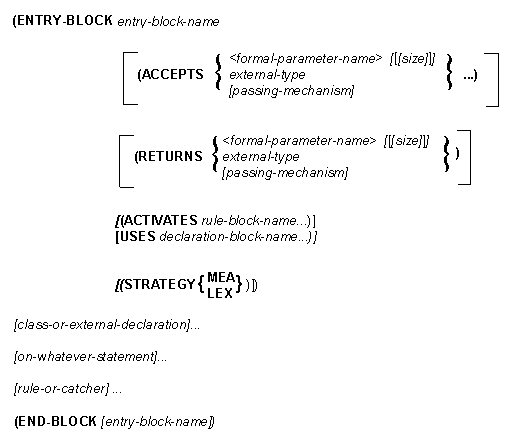
\includegraphics[scale=0.7]{f5-1}
  \caption{Entry Block Syntax}
  \label{f:5-1}
\end{figure}

The clauses within the \tt{ENTRY-BLOCK} declaration are all optional:

\begin{itemize}
\item The \tt{ACCEPTS} clause defines the input argument list, if
  any. If any argument is an array, its size is optional. See
  Chapter~\ref{c:otherlang} for information on external data types and
  passing mechanisms.
\item The \tt{RETURNS} clause specifies the entry block's return
  value, if any. If the return value is compound, its size can be
  either an input argument of an integer type (byte, short, and so on)
  or an integer constant. See Chapter~\ref{c:otherlang} 6 for
  information on external data types and passing mechanisms.
\item The \tt{ACTIVATES} clause enables rules not contained in the
  entry block to fire. See~\ref{}Rule Blocks for information on rule blocks.
\item The \tt{USES} clause allows rules contained in the entry block
  to match and manipulate objects whose class declarations are not
  contained in the entry block, and to call external routines whose
  declarations are not contained in the entry block. See~\ref{}Declaration
  Blocks for more information on declaration blocks.
\item The \tt{STRATEGY} clause allows you to specify a
  conflict-resolution strategy other than the default \tt{MEA}
  strategy.
\end{itemize}
  
An entry block may contain any RuleWorks program constructs except
another block construct, but they must be in the order shown above:
declarations first, then \tt{ON-} statements, then rules and catchers.

If an entry block contains \tt{OBJECT-CLASS} declarations, objects of
those classes can be matched only by rules contained in the block.  If
an entry block contains rules, those rules can fire only when the
block is active.  Declaration blocks and rule blocks allow you to
share objects and rules among multiple entry blocks.

The \tt{END-BLOCK} construct is required. \it{The entry-block-name} is
optional inside the \tt{END-BLOCK} construct, but if it is present the
compiler verifies that it is the same name as in the \tt{ENTRY-BLOCK}
construct.

\subsubsection{Calling an Entry Block}

When an entry block is called, that entry block is the only active
entry block. The entry block first runs its \tt{ON-ENTRY} actions (if
any), then runs recognize-act cycles until one of the following
occurs:
\begin{itemize}
\item The conflict set becomes empty, triggering the actions that were
  declared with the \tt{ON-EMPTY} statement (if any) followed by the
  actions that were declared with the \tt{ON-EXIT} statement (if any).
\item The \tt{RETURN} action is executed, triggering the actions that
  were declared with the \tt{ON-EXIT} statement (if any)
\end{itemize}

Entry blocks can call other entry blocks, and even call themselves
recursively. When an entry block is called, the caller is no longer
active. The caller is referred to as being \emph{suspended} and the
called block becomes the active block, just as with a routine in any
other language. Similarly, when the called block returns, the caller
becomes active again.

When an entry block returns, any objects created or changed by that
block remain in working memory (unless that entry block is the main
program, see~\ref{}Naming an Entry Block \tt{MAIN}, for details). If
that entry block is called again later, all of those objects are again
matchable. However, the objects cannot be matched or modified by any
other entry block unless both entry blocks are using the same
declaration block (see~\ref{}Declaration Blocks, for information on
declaration blocks).

\subsubsection{Scope of Arguments to an Entry Block}

The arguments received by an entry block are visible only to actions
within the \tt{ON-ENTRY}, \tt{ON-EVERY}, \tt{ON-EMPTY}, and
\tt{ON-EXIT} statements inside the entry block. They are not visible
to rules contained in or activated by the entry block. If rules need
to match input arguments, their values must be placed into one or more
objects (as shown in Example~\ref{e:5-1})

\begin{example}[!h]
\begin{quote}
\begin{verbatim}
; Shareable Class Declaration
(declaration-block numbers)
(object-class limit ^value)
(end-block numbers)

; Entry Point Declaration
(entry-block count_to
    (accepts <num-arg> long)
    (returns long)
    (uses numbers))

; Private Class Declaration
(object-class iterator ^count)

; Executable Constructs
(on-entry
    (bind <limit> (make limit ^value <num-arg>))
    (make iterator ^count 1))

(on-exit
    (remove <limit>) ; clean out WM when done
    (return <num-arg>))

(rule increment-rule
    (limit ^value <lim>)
    (iterator ^$id <it> ^count { <num> <= <lim> })
  -->
    (modify <it> ^count (<num> + 1)))

(rule now-done
    (limit ^$id <limit-id> ^value <lim>)
    (iterator ^$id <it> ^count > <lim>)
  -->
    (remove <it>)
    (remove <limit-id>))

(end-block count_to)
\end{verbatim}
\end{quote}
\caption{A Simple Entry Block and Declaration Block}
\label{e:5-1}
\end{example}

The same restrictions hold true of any variables bound in an \tt{ON-}
clause. Such variables are also visible within any \tt{ON-} clause.

\subsubsection{Scope of Execution of Entry Blocks}

A call frame is created when a RuleWorks entry block is called. It
contains all the dynamic data structures associated with a given
invocation of an entry block. That is, it consists of all of the
information ``local'' to this particular invocation of an entry block,
or in some way visible to this particular invocation. Calls and
returns really create and delete call frames. Call frames are an
integral piece of entry blocks; by themselves they have no names and
cannot be passed, returned, or otherwise manipulated directly.

The following are local to the call frame:
\begin{itemize}
\item Refraction.

  Refraction does not apply across invocations of entry blocks. Thus,
  a rule may fire more than once on the same data.  This could happen
  when an entry block calls itself recursively, or when one entry
  block calls another and both activate the same rule block, or when
  an entry block is called repeatedly.

\item The local rule-firing counter.

  This affects \tt{CATCH} statements. The \tt{CATCH} counter counts
  only rules fired in the entry block invocation in which the
  \tt{AFTER} action was executed, excluding rule firings in other
  invocations of the same entry block and in entry blocks called from
  the original entry block.
\end{itemize}

The following are global:
\begin{itemize}
\item The \verb|$ID| generator.

  The \verb|$ID| value of an object is universally unique across entry
  block invocations.

\item The time-tag counter.

  The time-tags assigned to objects are monotonically increasing
  across calls to and returns from entry blocks.

\item The global rule-firing counter.

  This affects the \tt{RUN} command when you provide an argument (for
  example, \tt{RUN} 5).  Rule firings from other entry blocks are
  counted.

\item The atom generator.

  This affects the RuleWorks \tt{GENATOM} and \tt{GENINT} functions,
  and the \verb|rul_genint|, \verb|rul_gensym|, and \verb|rul_gensymp|
  API routines.  Every atom generated for any of these routines is
  unique while the program is running, and is unique across your
  entire program, not merely within an entry block.
\end{itemize}

\subsubsection{Naming an Entry Block \tt{MAIN}}

An entry block named \tt{MAIN}, if supplied, is automatically
designated to the compiler and linker as the main RuleWorks
routine. This design has semantic parallelism with the C language and
provides the behavior most programmers would expect. The name can be
in any case.

If you want to capture command-line arguments to the program in a
portable way, a declaration in the following form is recommended:
\begin{quote}
\begin{verbatim}
(entry-block main
    (accepts <argc> long            ; traditional names for
             <argv> [<argc>] ASCIZ) ; command-line args
     ...)
\end{verbatim}
\end{quote}

\subsubsection{Returning a Value from an Entry Block}

RuleWorks provides an RHS action, \tt{RETURN} that stops the firing of
rules in the active entry block, executes the \tt{ON-EXIT} actions (if
any) and passes control back to the caller of the entry block. This
action has an optional argument, the value to be returned. The
argument can be any expression. Thus, the \tt{RETURN} action is useful
for returning a condition code or value (see Example~\ref{e:5-1}).

The \tt{RETURN} action is valid anywhere in the entry block, even
inside the \tt{ON-EXIT} and \tt{ON-EMPTY} statements. The \tt{RETURN}
action is valid only in an entry block; it is not valid in a rule
block.

Executing more than one \tt{RETURN} action in an entry block is
possible, for example, when an \tt{ON-EXIT} statement that contains a
\tt{RETURN} action is executed as a result of a \tt{RETURN} action in
a rule. If a value is being returned from the entry block, the value
of the last \tt{RETURN} action executed is used.

If the value returned by an entry block is an array, the memory
allocated for that array is not freed by RuleWorks. The following
example shows an entry block that accepts an array, sorts it, and then
returns it.

\begin{quote}
\begin{verbatim}
(entry-block sort_slowly
    (accepts <set-size> long
             <set>[<set-size>] asciz)
    (returns <sorted-set>[<set-size>] asciz))

; Return the input set, except sorted (albeit slowly)
(object-class an-atom ^value)

(object-class in-set ^values compound)

(object-class out-set ^values compound)

(on-entry
    (make out-set)
    (make in-set ^values <set>)
    (for-each <atom> in <set>
        (make an-atom ^value <atom>)))
(rule find-next
    (an-atom ^$id <atom> ^value <x>)
    -(an-atom ^$id <> <atom> ^value <= <x>)
    (out-set ^$id <out-set> ^values <out-vals>)
  -->
    (remove <atom>)
    (modify <out-set> ^values (compound <out-vals> <x>)))

(rule all-done
    (out-set ^$id <out-set> ^values <out-vals>)
    (in-set ^$id <in-set> ^values <in-vals>)
    -(an-atom)
  -->
    (remove <out-set> <in-set>)
    (write (crlf) | Sort of | <in-vals>
      (crlf) | ==> | <out-vals> (crlf))
    (return <out-vals>))

(end-block)
\end{verbatim}
\end{quote}

\section{Executing Actions Without Matching}

The actions on the right-hand side of a rule are executed only when
the left-hand side matches working memory and the resulting
instantiation is picked during conflict resolution. RuleWorks provides
two types of executable constructs whose actions are executed without
matching working memory: ``\tt{ON-}'' statements and catchers.

\subsubsection*{Using "\tt{ON-}" Statements}

RuleWorks entry blocks may contain one each of the four ``\tt{ON-}''
statements, which allow you to describe a set of actions that are
executed at certain points in the recognize-act cycle (see the figure,
``\tt{ON-}'' Statements and the Recognize-Act Cycle) without matching
any objects in working memory. These new statements are all defined
with names that begin with the prefix "\tt{ON-}" and end with the name
of the special condition under which their associated actions are
executed.

\begin{figure}
  \centering
  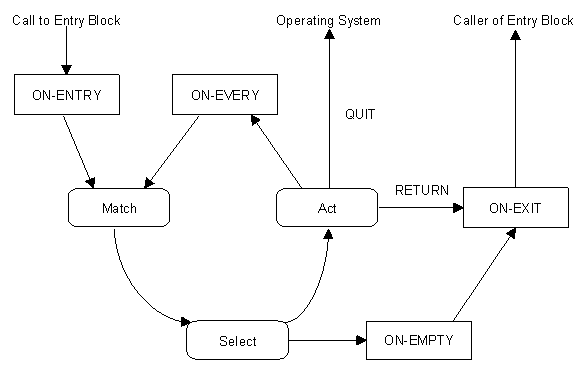
\includegraphics[scale=0.7]{f5-2}
  \caption{``\tt{ON-}'' Statements and the Recognize-Act Cycle}
  \label{f:5-2}
\end{figure}

The "\tt{ON-}" statements are listed below:
\begin{itemize}
  \item \tt{ON-ENTRY}

    The actions in an \tt{ON-ENTRY} statement are executed whenever
    its entry block is called, and before any rules can fire.  Thus,
    you can initialize working memory by putting \tt{MAKE} actions in
    your \tt{ON-ENTRY} statement. For example:

    \begin{quote}
\begin{verbatim}
(on-entry
    (bind <my_id> (make my_wmo)) ; Create the first WMO.
    (bind <rule_count> 0)        ; Initialize the counter...
    (bind <return_status> good)) ; ... and the return value.
\end{verbatim}
    \end{quote}

These \tt{MAKE} actions can use the input arguments to the entry block
(see the section of this chapter, Scope of Arguments to an Entry
Block)

The \tt{ON-ENTRY} statement is roughly analogous to the OPS5
\tt{STARTUP} statement.

\item \tt{ON-EVERY}

  The actions in an \tt{ON-EVERY} statement are executed immediately
  after each successful rule firing, and before the determination of
  the next rule to fire. If a rule is fired that has a \tt{RETURN} as
  its last action, then control will be returned up to the caller, and
  the \tt{ON-EVERY} actions will not be executed.

  You could use an \tt{ON-EVERY} statement to count the number of
  rules fired in the current invocation of the entry block, or to call
  an event handler. For example:
  \begin{quote}
\begin{verbatim}
(on-every
    (bind <rule-count> (<rule-count> + 1)))
\end{verbatim}
  \end{quote}
        
\item \tt{ON-EMPTY}

  The actions in an \tt{ON-EMPTY} statement are executed whenever it
  is time to select the next rule to fire and there are no rules
  eligible to fire and thus the conflict set is empty. Note that the
  run-time system does not execute any recognize-act cycles after an
  \tt{ON-EMPTY} statement, even if its actions create WMOs that
  satisfy one or more rules.

  You could use an \tt{ON-EMPTY} statement to return a failed status
  if the program should not have arrived at an empty CS.  For example:
  \begin{quote}
\begin{verbatim}
(on-empty
    (quit $failure))
\end{verbatim}
  \end{quote}
        
\item \tt{ON-EXIT}

  The actions in an \tt{ON-EXIT} statement are executed just before
  control is returned to the caller of the entry block. These actions
  are executed when control is returned via a \tt{RETURN} action or
  when the conflict set becomes empty. If an \tt{ON-EMPTY} statement
  was also specified, the \tt{ON-EXIT} actions are executed after the
  \tt{ON-EMPTY} actions, and immediately before control is returned to
  the calling routine.

  The \tt{ON-EXIT} actions are not executed after a \tt{QUIT} action
  or command.

  \tt{ON-EXIT} statements are useful for clean-up actions, such as
  removing dead instances of local object classes. For example:

  \begin{quote}
\begin{verbatim}
(on-exit
    (remove <my_id>)
    (remove-every local)
    (return <return_status>))
\end{verbatim}
  \end{quote}

\end{itemize}

\tt{ON-} statements must be contained in an entry block. They cannot
appear inside a rule block, nor inside a rule group within an entry
block (see Rule Blocks and Rule Groups for more information).

\begin{note}
  Any variables bound in one \tt{ON-} statement are available to all
  other \tt{ON-} statements. These variables are not available to any
  rules.
\end{note}

An entry block can contain at most one of each type of \tt{ON-}
statement. It doesn't have to contain any of them.

\subsubsection*{Using a Catcher}

A \emph{catcher} is a list of actions that are executed after a
specified number of recognize-act cycles have been executed. For
example, if program execution is unattended, as in a batch job, a
catcher can halt the program if it does not produce results within a
specified limit.

You define a catcher with a \tt{CATCH} statement, which includes a
symbol and one or more actions. The symbol names the catcher, and
functions as a label. A catcher's name must be unique; that is, it
cannot be the same as the name of another catcher, rule, or rule group
in the program. When the catcher fires, the actions are executed.

The following \tt{CATCH} statement defines a catcher named
\tt{FINISH}, which consists of two actions, \tt{WRITE} and \tt{HALT}:

\begin{quote}
\begin{verbatim}
(catch finish
    (write (crlf) |Finished.|)
    (halt))
\end{verbatim}
\end{quote}

You enable a catcher with the \tt{AFTER} action, which tells the
run-time system when to execute the catcher. Specify the \tt{AFTER}
action with a positive integer and the name of the catcher you want to
enable. The integer indicates the number of recognize-act cycles (of
the current invocation of the entry block) that the run-time system is
to execute before executing the specified catcher. For example:

\begin{quote}
\begin{verbatim}
(after 10 finish)
\end{verbatim}
\end{quote}

Only one catcher can be enabled at a time, per call frame. Therefore,
when you enable a catcher, you disable the catcher currently enabled
(if any). Catchers are automatically disabled after they have been
executed.

Catchers may be contained in either entry or rule blocks. The catcher
must be contained in the same block as the \tt{AFTER} action that
enables it.

The following example illustrates the use of two catchers,
\tt{STARTER} and \tt{FINISH}.

\begin{quote}
\begin{verbatim}
(entry-block sample)

(object-class start) ; Used for initialization

(object-class number ^value) ; Contains value to be printed

(on-entry
    ; Creates a working-memory object (START)
    (make start)
    ; Enables catcher STARTER after 1 recognize-act cycle
    (after 1 starter))

(2) (catch starter ; Catcher STARTER
        (write (crlf) |Counting to 10...|)
        (make number ^value 1)
        ; Enables catcher FINISH after the run-time
        (after 10 finish))

    ;system has executed 10 more cycles
(4) (catch finish ; Catcher FINISH
        (write (CRLF) |Finished.|)
        (return)) ; Stop program

(1) (rule initialize ; Initialize working memory
        (start ^$id <START>)
      -->
        (write (crlf) |Starting...|)
        (remove <start>))

(3) (rule count ; Output numbers
        (number ^$id <number> ^value <n>)
      -->
        (write (crlf) (rjust 5) <n>)
        (modify <number> ^value (<n> + 1)))

(end-block sample)
\end{verbatim}
\end{quote}

This program produces the following output:

\begin{quote}
\begin{verbatim}
Starting...
Counting to 10...
     1
     2
     3
     4
     5
     6
     7
     8
     9
     10
Finished.
\end{verbatim}
\end{quote}

\tt{STARTER} and \tt{FINISH} are as follows:
\begin{itemize}
\item[\tt{(1)}] The first recognize-act cycle fires rule
  \tt{INITIALIZE}, because its CE matches the \tt{START} object
  created in the \tt{ON-ENTRY} statement. The \tt{ON-ENTRY} statement
  does not count as a cycle.

\item[\tt{(2)}] Catcher \tt{STARTER} fires after one recognize-act
  cycle has been executed. \tt{STARTER} is enabled in the
  \tt{ON-ENTRY} statement.

\item[\tt{(3)}] The \tt{MAKE} action in catcher \tt{STARTER} creates
  an object on which rule \tt{COUNT} can fire.

\item[\tt{(4)}] The \tt{AFTER} action in catcher \tt{STARTER} enables
  catcher \tt{FINISH} to fire after ten more recognize-act cycles have
  been executed.
\end{itemize}

\section{Declaration Blocks}

Declarations (\tt{OBJECT-CLASS} and \tt{EXTERNAL-ROUTINE}) can be
private or shareable.  A declaration is private if it is contained in
either an entry block or a rule block. Objects whose class declaration
is private to a block can be matched only by rules contained in that
block. In other words, by placing declarations inside an entry block
or rule block you create private data for that block. Similarly,
external routines whose declarations are local to a block can be
called from inside that block only.

Figure~\ref{f:5-3} shows a RuleWorks program that consists of one
entry block with two private object class declarations. Rules in
\tt{EB1} can ``see'' all objects of classes \tt{Y} and \tt{Z}.

\begin{figure}[h]
  \centering
  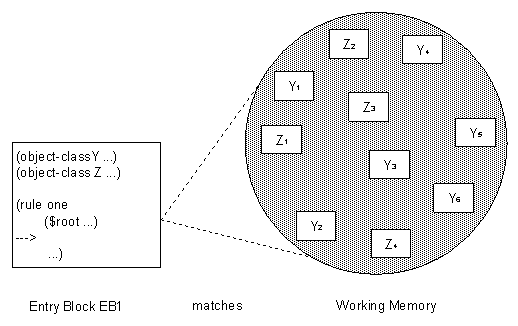
\includegraphics[scale=0.7]{f5-3}
  \caption{Private Data in RuleWorks}
  \label{f:5-3}
\end{figure}

\subsubsection{Data Partitioning}

By default, RuleWorks partitions working memory so there is no
conflict over object classes of the same name when two or more entry
blocks are combined. Rules can match only objects whose classes are
contained in or used by their entry block; all other objects are
invisible.

This invisibility includes matches against the built-in class
\verb|$ROOT|. If an object class is not visible at compile-time,
instances of it are not visible to the block at run-time.

\subsubsection{Declaration Sharing}

A \emph{declaration block} allows you to create a collection of
declarations that are \emph{shareable} among multiple entry blocks or
rule blocks.  \emph{Declaration sharing} allows you to explicitly
decide which data should remain private and which should be shared
(and the extent of that sharing). This allows the absolute
partitioning of object class declarations between several
independently-developed subsystems of an application. It also allows
information to be restricted to a single routine or a set of
interdependent routines.

A declaration block consists of zero or more declarations bounded by a
\tt{DECLARATION-BLOCK} construct at the top and an \tt{END-BLOCK}
construct at the bottom.

\begin{quote}
\begin{verbatim}
(declaration-block line-items)
    (object-class item ^item-code
        ^item-name
        ^quantity
        ^price-per
        ^item-total)
    (object-class shippable-item
        (inherits-from item)
        ^part-number)

 (end-block line-items)
\end{verbatim}
\end{quote}

The complete syntax of a declaration block is shown below:
\begin{quote}
\verb|(|\tt{declaration-block} \it{decl-block-name}\verb|)|\par
\qquad[\it{class-or-external-declaration}] \ldots\par
\verb|(|\tt{end-block} [\it{decl-block-name}]\verb|)|
\end{quote}
 
The \it{decl-block-name} is required in the \tt{DECLARATION-BLOCK}
construct. It is optional in the \tt{END-BLOCK} construct, but if
supplied it is checked. Declaration block names must be no longer than
31 characters, and contain letters, digits, and underscores only.
Declaration block names must be distinct from entry and rule block
names. Finally, the first eight characters of all declaration block
names used in a program must be unique. This allows RuleWorks to
create portable names for the compiled files. For example, having two
declaration blocks named \verb|DECLARE_CONTROL| and
\verb|DECLARE_KIWI| generates a compile-time warning and results in a
single file called \verb|DECLARE_.USE|. Naming the blocks
\verb|CONTROL_DECLS| and \verb|KIWI_DECLS| correctly generates two
\verb|.USE| files.

\begin{note}
  Object classes that are related by inheritance must all be declared
  in the same block. An object class cannot inherit from a class
  declared in some other block.
\end{note}

A declaration block must not contain any executable statements (rules,
\tt{ON-} statements, or catchers).

Declarations are shared via the \tt{USES} clause of an
\tt{ENTRY-BLOCK} or \tt{RULE-BLOCK} construct.  Objects whose class
declarations are shared by a block are just as visible to the rules
within that block as objects whose declarations are private to that
block. Note that a \tt{USES} clause cannot specify individual class
names, only declaration block names.

A block can use more than one declaration block. A compile-time error
occurs if the combined shared and private declarations contain any
classes with identical names.

Figure~\ref{f:5-4} shows some private and some used object class
declarations. The \tt{USES} clause in \tt{EB1} ``pulls in'' the
declarations from \tt{DB1}.  Rules in \tt{EB1} can still match objects
of classes \tt{Y} and \tt{Z}.

\begin{figure}[h]
  \centering
  
\includegraphics[scale=0.5]{f5-4}
  \caption{Shareable Declaration Blocks}
  \label{f:5-4}
\end{figure}

Figure~\ref{f:5-5} shows two entry blocks in the same program, each
with some private and some used object class declarations. Rules in
\tt{EB1} can see objects of classes \tt{Y} and \tt{Z} only; rules in
\tt{EB2} can see objects of classes \tt{W} and \tt{X} only.

\begin{figure}[h]
  \centering
  
\includegraphics[scale=0.5]{f5-5}
  \caption{Two Shareable Declaration Blocks}
  \label{f:5-5}
\end{figure}

Figure~\ref{f:5-6} shows the same two entry blocks sharing an object
class declaration. Rules in \tt{EB1} can see objects of classes
\tt{Y}, \tt{Z}, and \tt{O}; rules in \tt{EB2} can see objects of
classes \tt{W}, \tt{X}, and \tt{O}.

\begin{figure}[h]
  \centering
  
\includegraphics[scale=0.5]{f5-6}
  \caption{Shared Data in RuleWorks}
  \label{f:5-6}
\end{figure}

The declaration block(s) used by an entry block must be compiled
before the entry block itself can be compiled. You can put declaration
blocks in a different file and compile them separately, or you can
place them in the same file but above the entry block. In either case,
compiling a declaration block results in an intermediate file with the
extension \tt{.USE}. Entry or rule blocks in other source files can
subsequently use one or more of those declaration blocks, without
seeing all of the other declarations that were in the original source
file.

The following example shows a more complex set of block constructs where both
declarations and rules are being shared.

\begin{quote}
\begin{verbatim}
(declaration-block common_decls)
    (object-class C-1 ...)
    (object-class C-2 ...)
(end-block common_decls)

(entry-block my_little_function
    (accepts ...)
    (activates shared-rules-1)
    (uses common_decls))
    ; needed to expose the contents of the
    ; declaration-block defined above

(rule my-rule-1 ...)
...

(end-block my_little_function)

(rule-block shared_rules_1
    (uses common_decls))

(rule my-rule-1 ...)
...

(end-block shared_rules_1)

(rule-block shared_rules_2
    (uses common_decls))
...

(end-block shared-rules-2)

(entry-block my_other_little_function
    (accepts ...)
    (activates shared-rules-1 shared-rules-2)
    (uses common_decls))

(rule my-rule-1 ...)
...

(end-block my_other_little_function)
\end{verbatim}
\end{quote}

\subsubsection*{Calling a Declaration Block}

Declaration blocks are callable, and in certain circumstances it may
be necessary to call one. For example, the following C program calls
an entry block named \verb|KBT_RULES| that uses a declaration block
named \verb|KBT_DECL|. In order for the C program to initialize
working memory before calling the entry block, it must first call the
declaration block:

\begin{quote}
\begin{verbatim}
#include <stdio.h>
#include <rul_rtl.h>

main ()
{
    /* define RuleWorks stuff */
    rul_atom obj_id;

    printf("Calling RuleWorks...");

    /* initialize working memory */
    KBT_DECL();

    /* make one object */
    rul_make_instance("(AnyWin ^name testing)","KBT_DECL");
    /* call RuleWorks entry block */
    kbt_rules();
}
\end{verbatim}
\end{quote}

\section{Rule Blocks}

In RuleWorks, rules can be gathered together into \emph{rule
  blocks}. A rule block is a collection of rules that may be shared
among several entry blocks. Whenever \emph{any} of the entry blocks is
called, all the rules in the rule blocks it activates will participate
in matching and be enabled to fire.

Rule blocks can also be used when the number of rules in a single
entry block becomes too large to reasonably store in a single file.
You can have rule blocks that are activated by only one entry block.

The complete syntax of a rule block is shown in Figure~\ref{f:5-7}.

\begin{figure}[h]
  \centering
  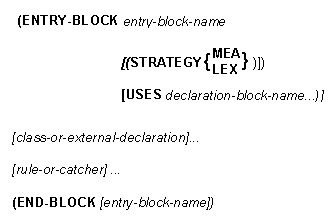
\includegraphics[scale=0.7]{f5-7}
  \caption{Complete Syntax of Rule Block}
  \label{f:5-7}
\end{figure}

Rule blocks are activated by entry blocks with the \tt{ACTIVATES}
clause. Only rules contained in or activated by the active entry block
are eligible for matching and firing. Only entry blocks can activate
rule blocks; one rule block can neither contain nor activate another.

The \it{rule-block-name} is required in the \tt{RULE-BLOCK}
construct. It is optional in the \tt{END-BLOCK} construct, but if
supplied it is checked. Rule block names must be no longer than 31
characters, and contain letters, digits and underscores only. Rule
block names must be distinct from entry and declaration block names.

Each rule block can have it's own \tt{STRATEGY} clause. However, all
rule blocks used by an entry block must have the same strategy as the
entry block. It is a run-time error to activate rule blocks that have
different strategies. If no strategy clause is specified, the default
is \tt{MEA}.

A rule cannot be in more than one rule block; a rule block can contain
zero or more rules.  (An empty rule block can be useful during
prototyping and/or stuibbing phase of development). Note that all
rules contained in a block must be in the same file, but a file can
contain more than one block. Rule blocks can be compiled before or
after the entry block that activates them.

\begin{note}
  A rule block is not a directly callable entity, and should not be
  called from any language except RuleWorks. If a rule block is not
  referenced by at least one entry block, it's rules can never
  fire. No rules can be shared among multiple entry blocks unless they
  are contained within a rule block.
\end{note}

Rule blocks are activated by entry blocks by the \tt{ACTIVATES} clause
(see Entry Blocks). Only rules contained in or activated by the active
entry block are eligible for matching and firing. Only entry blocks
can activate rule blocks; one rule block can neither contain nor
activate another.

The visibility of objects to the active rules depends on whether their
blocks contain or use the corresponding \tt{OBJECT-CLASS}
declarations.  When you put rules in rule blocks, it is up to you to
set up declaration blocks in such a way that the classes that are to
be matched and modified in your entry and rule blocks are shared as
appropriate. There is no implicit sharing of declarations between an
entry block and the rule blocks it activates. Thus, in the example,
Sharing Declarations and Rules, the clause is required in the rule
block as well as in the entry blocks.

\section{Scope of Names}

In RuleWorks, the name space for declarations and executable
statements is not global. This name space is divided by blocks into
independent name spaces.

\begin{itemize}
\item Within a block, all named constructs except external routines
  share the same name space. Therefore, no rule can have the same name
  as another rule, rule-group, or catcher in that same
  block. Different blocks can, however, each contain a rule with the
  same name.

  This name space is enforced by the RuleWorks compiler, and permits
  names to be any legal symbol.

  When an entry block activates rule blocks, the entry block and all
  the rule blocks still have separate name spaces.

\item Object classes inhabit a second name space, which is also
  enforced by the RuleWorks compiler. You can have an object class and
  a rule with the same name, but you cannot have an object class and
  an external routine with the same name.

  When an entry block or a rule block uses declaration blocks, the
  using block and all the used blocks have one common name space for
  object classes and external routines.

\item Block names and external routine names share a third name space,
  which is enforced by the platform linker. For example, a rule block
  cannot have the same name as an entry block, declaration block, or
  external routine called by the same program.
\end{itemize}
  
\section{Rule Groups}

Within an entry or rule block, an additional level of structure can be
imposed on a collection of rules by using the \tt{RULE-GROUP}
construct. This extra level is not necessary for program execution,
but it can enable some useful debugging information.

\section{Efficiency Issues}

The entry block system in RuleWorks may cause a program speed
\emph{increase} because it restricts the visibility of rules and
objects to what you specified, rather than the global visibility of
OPS5.

Only those programs that actually use the block system will see the
efficiency improvement. Programs that are converted from OPS5 by
wrapping a single entry block around all of the rules will not see
this improvement.

The entry block system may impose an efficiency penalty when entry
blocks are called repeatedly. To avoid this problem, you should
compile any entry block that is called repeatedly with the Optimize
qualifier set to \tt{REINVOCATION}. Note that the RuleWorks language
semantics are not affected by this qualifier, only entry block
initialization run-time and maximum memory usage.

Partitioning working memory with declaration blocks will, if done
appropriately, provide a significant improvement in execution speed.

%%% Local Variables:
%%% mode: latex
%%% TeX-master: "rwug"
%%% End:

\chapter{Using RuleWorks with Other Languages}
\label{c:otherlang}

Programming tasks such as computing mathematical expressions,
manipulating strings, and editing large quantities of data are often
easier and more efficient to develop in languages other than
RuleWorks. If you are developing a RuleWorks program that needs to
perform these types of tasks, you should consider using external
routines. An external routine is a function or subroutine written in a
language other than RuleWorks.  External routines include prewritten
routines such as system services and run-time library (RTL) routines.

RuleWorks allows external routines that accept arguments and return
results according to the hardware platform's calling standard. This
means that you can call external routines that are not written
specifically for RuleWorks. Example~\ref{e:6-1} shows a simple
RuleWorks program calling the C RTL routine, \verb|sqrt|.

\begin{example}[h]
\begin{quote}
\begin{verbatim}
(declaration-block decls)

(object-class start)

(end-block decls)

(entry-block main
    (uses decls)

(on-entry
    (make start)))

(external-routine sqrt
    (accepts double-float)
    (returns double-float))

(rule square-root
    (start)
  -->
    (write |Enter a number> |)
    (bind <input> (accept-atom))
    (write |The square root is| (sqrt <input>)))

(end-block main)
\end{verbatim}
\end{quote}
\caption{Calling an External Routine from RuleWorks}
\label{e:6-1}
\end{example}

RuleWorks also allows entry blocks to be called from other
languages. Entry blocks can accept arguments and return a value. Entry
blocks can call other entry blocks, but the callers must declare the
other entry blocks with \tt{EXTERNAL-ROUTINE} declarations. Entry
blocks can even call themselves recursively.

\section{Calling External Routines from RuleWorks}

You must declare external routines before you call them in your
RuleWorks program.  External routines are scoped to the block in which
they are declared.

The easiest way to ensure that the correct declarations have been made
is to place the \tt{EXTERNAL-ROUTINE} declarations in a separate
declaration block and have each module acquire the compiled
declarations via a \tt{USES} clause. See Chapter~\ref{c:program} for
details on data partitioning and declaration sharing.

The complete syntax for the \tt{EXTERNAL-ROUTINE} declaration is shown
in the following:

\begin{quote}
\tt{(EXTERNAL-ROUTINE} \it{routine-name}\par
\qquad[\tt{(ALIAS-FOR} \it{actual-routine-name}\tt{)}]\par
\qquad\qquad[\verb|<|\it{formal-parameter-name}\verb|>| [\tt[\it{size}\tt]]]\par
\qquad[\tt{(ACCEPTS} \{\it{external-type}\} \ldots\verb|)|]\par
\qquad\qquad[\it{passing-mechanism}]\par
\qquad\qquad[\verb|<|\it{formal-parameter-name}\verb|>| [\tt[\it{size}\tt]]]\par
\qquad[\tt{(ACCEPTS} \{\it{external-type}\}\tt{)}]\par
\qquad\qquad[\it{passing-mechanism}]\par
\end{quote}

The \it{routine-name} is required; the \tt{ALIAS-FOR}, \tt{ACCEPTS}
and \tt{RETURNS} clauses are optional.  The syntax for calling an
external routine is shown below:

\begin{quote}
\verb|(|\it{routine-name} [\{\it{value-expression}\} \ldots]\verb|)|
\end{quote}

\tt{EXTERNAL-ROUTINE} declarations may appear inside any type of block, but
they must appear inside of some kind of block, and they must appear
before they are used. Duplicate declarations of the same external
routine will generate a warning and be ignored so long as the
declarations are identical.

External routines that return a value can be used on the RHS (as shown
in Example~\ref{e:6-1}) or on the LHS. External routines that do not return a
value must be used on the RHS as if they were RuleWorks actions. You
can also call an external routine that does return a value as if it
were an RHS action, but in this case RuleWorks ignores the return
value.

\subsubsection{Writing Portable Code}

The \tt{ALIAS-FOR} clause allows you to declare that the routine name
used inside RuleWorks is not the actual name that will be linked. This
is useful for mapping a case-sensitive external routine name onto a
case-insensitive RuleWorks symbol.

The actual function name must be quoted to preserve case. For example:

\begin{quote}
\begin{verbatim}
(external-routine xt_parent ; routine name used inside TINpan
    (alias-for |XtParent|)  ; actual function name
    (accepts pointer)
    (returns pointer))
\end{verbatim}
\end{quote}

You can use at most one \tt{ALIAS-FOR} clause in an \tt{EXTERNAL-ROUTINE}
declaration. You must provide exactly one function name in an
\tt{ALIAS-FOR} clause.

\subsubsection{Passing Parameters}

Use the \tt{ACCEPTS} clause to declare one or more parameters for an
external routine. The \verb|<|\it{formal-parameter-name}\verb|>| is
optional; use it to help make your code more self-documenting. The
external-type-name is required. The passing-mechanism for each
argument is also optional; the default mechanism for each external
type is shown in Table~\ref{t:6-1}. Arrays of each type are also
allowed, passed \tt{BY REFERENCE} only.

\begin{table}[h]
  \begin{tabularx}{\columnwidth}{lXXX}
    \toprule
    & \multicolumn{3}{c}{Argument Passing Mechanisms} \\
    \midrule
    External Data Type & \tt{BY VALUE} & \tt{BY REFERENCE READ-ONLY} & \tt{BY REFERENCE READ-WRITE} \\ 
    \tt{BYTE} & Default & * & * \\
    \tt{SHORT} & Default & * & * \\
    \tt{LONG} & Default & * & * \\
    \tt{UNSIGNED-BYTE} & Default & * & * \\
    \tt{UNSIGNED-SHORT} & Default & * & * \\
    \tt{UNSIGNED-LONG} & Default & * & * \\
    \tt{SINGLE-FLOAT} (1) & Default  &      *       &      * \\
    \tt{DOUBLE-FLOAT} (2) & Default  &      *       &      * \\
    \tt{ASCIZ} & N/S      &   Default    &      * \\
    \tt{ASCID} & N/S      &   Default    &      * \\
    \tt{POINTER} (3) & Default  &      *       &      * \\
    \tt{ATOM} (4) & Default  &      *       &      * \\
    \bottomrule
  \end{tabularx}
  \begin{quote}
    (1) On VMS systems, \tt{SINGLE-FLOAT} refers to
    \verb|F_float_data|

    (2) On VAX VMS systems, \tt{DOUBLE-FLOAT} refers to
    \verb|D_float data|; on OpenVMS for Alpha AXP systems,
    \tt{DOUBLE-FLOAT} refers to \verb|G_float| data.

    (3) Opaque virtual address

    (4) Opaque atom

    * Supported, but not the default

    N/S Not supported
  \end{quote}
  \caption{External Data Types and Argument-Passing Mechanisms}
  \label{t:6-1}
\end{table}

Numeric and pointer external types default to zeros. \tt{ASCIZ} and
\tt{ASCID} externals default to the zero-length string. The \tt{ATOM}
external defaults to \tt{NIL}.

RuleWorks's compound values correspond to an array of atoms in
external routines. You declare a parameter as an array by putting
brackets (\verb|[]|) between the formal parameter name and the external
data type. If you do not declare the size of the array by putting an
integer between the brackets, then the array received by the external
routine has as many elements as the compound value had when it was
passed out, and the external routine cannot change the size of the
array. An array returned by an external routine must be the declared
size.

Since the size of the array is not automatically passed, applications
using empty brackets must define a convention such as a specific value
to signal the end of the array, or pass the length as a separate
parameter. Example~\ref{e:6-2} shows a C program that passes a
compound value.

\begin{example}[!h]
\renewcommand{\baselinestretch}{0.9}
\begin{quote}
\begin{verbatim}
#include <stdio.h>
#include <rul_rtl.h>

/* Function: concat_compound
 *
 * Accepts: The length of the array passed as the second argument
 *   An array of asciz strings
 * Function: Constructs a string containing the values in a compound.
 * Example:
 *   Given arguments: 3 and ("A","B","C")
 *   it returns the string "A-B-C"
 * Side Effect:
 *   Prints out all the input strings in the second argument,
 *   assuming that they all fit into one symbol.
 * Returns
 *   The string formed by concatenating all the elements of the
 *   compound, assuming that they will all fit into a symbol.
 *   If they do not fit into a symbol, the result is truncated
 *   at the maximum symbol size.
 */
char *concat_compound (long num_elements, char *az_array[])
{
    int  i, index, len;
    static char result[RUL_C_MAX_SYMBOL_SIZE+1];
    index = 0;
    printf ("\n Elements found in compound:");
    for ( i=0; i<num_elements; i++) {
        len = strlen (az_array[i]);
        if (len > RUL_C_MAX_SYMBOL_SIZE - index)
            len = RUL_C_MAX_SYMBOL_SIZE - index;
        strncpy (&result[index], az_array[i], len);
        index = index + len;
        if (index >= RUL_C_MAX_SYMBOL_SIZE) {
            /* not enough space in a symbol for all the compound values */
            result[RUL_C_MAX_SYMBOL_SIZE] = '\0';
            return (&result);
        }
        if ((i + 1) < num_elements) {
            /* insert a dash between compound values */
            result[index] = '-';
            index = index + 1;
        }
        printf ("\n %s", az_array[i]);
    }
    if (index < RUL_C_MAX_SYMBOL_SIZE+1) {
        result[index] = '\0';
    }
    return (&result);
}
\end{verbatim}
\end{quote}
\caption{Passing a Compound Value: C Function}
\label{e:6-2}
\end{example}

Example~\ref{e:6-3} shows the RuleWorks program that calls the C function in
Example~\ref{e:6-2}.

\begin{example}[h]
\begin{quote}
\begin{verbatim}
(entry-block main

(object-class classname ^comp-attr compound ^length ^atom)

(external-routine concat_compound
    (accepts <comp_len> long by value
             <az_array> [] asciz by reference read-only)
    (returns <ret_asciz> asciz))

(external-routine strlen
    (accepts <az_string> asciz)
    (returns <length> long))

(on-entry
    (make classname ^comp-attr (compound a b c)))

(rule call-C-function
    (classname ^$id <obj> ^atom <sym> ^length <> (strlen <sym>)
         ^comp-attr <comp>)
  -->
    (bind <result> (concat_compound (length <comp>) <comp>))
    (write (crlf) | | <comp> |==>| <result>)
    (remove <obj>))

(end-block main)
\end{verbatim}
\end{quote}
\caption{Passing a Compound Value: RuleWorks Program}
\label{e:6-3}
\end{example}

The dialog in the following example illustrates compiling, linking,
and running Example~\ref{e:6-2} and Example~\ref{e:6-3} on a VMS
system.

\begin{quote}
\begin{verbatim}
$rulework concat
...
$cc concat_comp
$link concat,concat_comp,rul$library:rul_rtl/lib
$run concat
Elements found in compound:
     A
     B
     C
     A B C ==> A-B-C
\end{verbatim}
\end{quote}

\subsubsection{Passing Non-Atomic RuleWorks Objects}

In RuleWorks, there are several kinds of objects with no corresponding
entity in external routines. These objects cannot be passed directly,
but they can be passed indirectly. They are listed below with the
indirect mechanism by which they can be passed.

\begin{table}[h]
  \begin{tabularx}{\columnwidth}{lX}
    \toprule
    Object & Indirect Passing Mechanism \\
    \midrule
    WMO & By object identifier, using the external type
          \tt{POINTER} or \tt{ATOM} \\
    Compound value & By converting it into an array \\
    \bottomrule
  \end{tabularx}
  \caption{Passing Non-Atomic Objects}
  \label{t:6-2}
\end{table}

\subsubsection{External Data Types}

Values in RuleWorks are converted into external data types whenever
they are passed to any external routine. These conversions are done
automatically based on the \tt{EXTERNAL-ROUTINE} declarations. The
type specifications are checked at compile time for constants and at
run time for expressions. Table~\ref{t:6-3} shows which RuleWorks
types can be passed for each external type.

\begin{table}[h]
  \begin{tabularx}{\columnwidth}{l|lllll}
    \toprule
    & \multicolumn{5}{c}{RuleWorks Type} \\
    \midrule
    External Type   & \tt{INTEGER}    & \tt{FLOAT} & \tt{SYMBOL} & \tt{INSTANCE-ID} & \tt{OPAQUE} \\
    \midrule
    \tt{BYTE}            & Natural    & Implicit   & Error      & Error       & Error   \\
    \tt{SHORT}           & Natural    & Implicit   & Error      & Error       & Error   \\
    \tt{LONG}            & Equivalent & Implicit   & Error      & Error       & Error   \\
    \tt{UNSIGNED-BYTE}   & Natural    & Implicit   & Error      & Error       & Error   \\
    \tt{UNSIGNED-SHORT}  & Natural    & Implicit   & Error      & Error       & Error   \\
    \tt{UNSIGNED-LONG}   & Natural    & Implicit   & Error      & Error       & Error   \\
    \tt{SINGLE-FLOAT} (1) & Implicit   & Natural    & Error      & Error       & Error   \\
    \tt{DOUBLE-FLOAT} (2) & Implicit   & Equivalent & Error      & Error       & Error   \\
    \tt{ASCID}           & Implicit*  & Implicit*  & Equivalent & Implicit*   & Error   \\
    \tt{ASCIZ}           & Implicit*  & Implicit*  & Equivalent & Implicit*   & Error   \\
    \tt{POINTER}         & Error      & Error      & Error      & Error       & Natural \\
    \tt{ATOM} & \multicolumn{5}{c}{No conversion required for \tt{ATOM}s} \\
    \bottomrule
  \end{tabularx}
  \begin{quote}
    (1) On VMS systems, the external type \tt{SINGLE-FLOAT} refers to
    \verb|F_float| data

    (2) On VAX VMS systems, the external type \tt{DOUBLE-FLOAT} refers
    to \verb|D_float data|; on OpenVMS for Alpha AXP systems, to
    \verb|G_float|.

    * \tt{ASCID} and \tt{ASCIZ} values are coerced outbound only. All
    other entries in this table apply both to calling out from and
    calling in to RuleWorks
  \end{quote}
  \caption{Type Conversions of External Routine Parameters}
  \label{t:6-3}
\end{table}

The ``natural'' type conversion referred to in Table~\ref{t:6-3} is
the one used when external data is returned to RuleWorks in a
\tt{READ-WRITE} parameter. The ``equivalent'' RuleWorks type/external
type pairs have no loss of precision when passed either way as a
\tt{READ-WRITE} parameter. The ``implicit'' type conversions are
handled automatically by RuleWorks according to the declarations. For
example, you can pass an \tt{INTEGER} atom as a \tt{SINGLE-FLOAT},
\tt{DOUBLE-FLOAT}, \tt{ASCIZ}, or \tt{ASCID} parameter without using
the \tt{FLOAT} or \tt{SYMBOL} conversion functions. However, passing a
\tt{SYMBOL} or \tt{INSTANCE-ID} as any numeric external type causes an
error.

``Outbound only'' means that when an \tt{INTEGER}, \tt{FLOAT}, or
\tt{INSTANCE-ID} atom is passed from RuleWorks to an external routine
that expects a string, the value is coerced.  However, if that string
is returned (as a \tt{READ-WRITE} parameter), it becomes an atom of type
\tt{SYMBOL}.

A compound value can be passed only as an array, and only a compound
can be passed as an array. Each atom within the compound must be
compatible (according to Table~\ref{t:6-3}) with the external type.

If the external type is not large enough to represent the value being
passed out, a warning is signaled. For example, 300 should not be
passed out to an external routine that expects a byte.

Example~\ref{e:6-5} and Example~\ref{e:6-6} show how to return a
compound value, and how to use a \tt{READ-WRITE} parameter.

\begin{example}{!h}
\begin{quote}
\begin{verbatim}
#include <stdio.h>
#include <rul_rtl.h>

/* Example function explode
 *
 * Accepts:
 * An asciz string
 * Function:
 * Turns a symbol into an array of characters.
 * Example:
 * Given the argument "HELLO"
 * Writes 5 into the second argument and
 * Returns "H", "E", "L", "L", "O", "", "", ...
 * Side Effect:
 * Modifies the write-only argument, num_returned.
 * Returns
 * An array (rul_c_max_symbol_size in length)
 * of very short ASCIZ strings
 * (at most one character each).
 */

char **explode (char *in_string, long *num_returned)
{
    /* The actual string space */
    static char short_strings[RUL_C_MAX_SYMBOL_SIZE][2] ;
    /* The array of string pointers to be returned */
    static char *exploded[RUL_C_MAX_SYMBOL_SIZE] ;
    static long called_before = FALSE ;
    long i ;
    if (! called_before) {
        /*
        ** On the first invocation of this function, set up
        ** the array of string pointers.
        */
        for (i=0; i<RUL_C_MAX_SYMBOL_SIZE; i++) {
            short_strings[i][1] = '\0' ;
            exploded[i] = &(short_strings[i][0]) ;
        }
        called_before = TRUE ;
    }

    /*
    ** For each character in the input string, create an
    ** entry in the array of strings to be returned.
    */
    *num_returned = strlen(in_string) ;
    for (i=0; i<RUL_C_MAX_SYMBOL_SIZE; i++) {
        if (i < *num_returned) {
        short_strings[i][0] = in_string[i] ;
        } else {
        short_strings[i][0] = '\0' ;
        }
    }
    return (exploded) ;
}
\end{verbatim}
\end{quote}
\caption{External Function That Returns an Array}
\label{e:6-5}
\end{example}


\begin{example}{!h}
\begin{quote}
\begin{verbatim}
(entry-block main)

(external-routine explode
    (alias-for |explode|)
    (accepts <string> asciz
             <count> long by reference read-write)
    (returns <strings>[256] asciz))
 
(object-class name ^as-word ^as-compound compound)

(on-entry
    (make name ^as-word abc)
    (make name ^as-word |hello|)))

(rule explode-it
    (name ^$id <n-id> ^as-word { <> NIL <word> } ^as-compound [=] 0)
  -->
    (bind <ret-len> 0)
    (bind <ret-list> (explode <word> <ret-len>))
    (modify <n-id> ^as-compound (subcompound <ret-list> 1 <ret-len>)))

(end-block main)
\end{verbatim}
\end{quote}
\caption{RuleWorks Program That Passes a READ-WRITE Parameter}
\label{e:6-6}
\end{example}

The dialog in Example~\ref{e:6-7} shows what happens when you run the
RuleWorks program in Example~\ref{e:6-6}.

\begin{example}{!h}
\begin{quote}
\begin{verbatim}
RuleWorks> trace on wm
RuleWorks> run 2
<=WM: #2 2 [NIL] (NAME ^AS-WORD hello)
=>WM: #2 3 [EXPLODE-IT] (NAME ^AS-WORD hello ^AS-COMPOUND (COMPOUND h e l l o))
<=WM: #1 1 [NIL] (NAME ^AS-WORD ABC)
=>WM: #1 4 [EXPLODE-IT] (NAME ^AS-WORD ABC ^AS-COMPOUND (COMPOUND A B C))
%RUL-I-PAUSE, Pausing after running requested number of rules
RuleWorks>
\end{verbatim}
\end{quote}
\caption{Passing a \tt{READ-WRITE} Parameter}
\label{e:6-7}
\end{example}

\begin{note}
  Whenever a \tt{SYMBOL} is converted to a string to be passed to an
  external routine, the string passed contains the print form of the
  symbol. Thus, in Example~\ref{e:6-6}, the quoted symbol, \verb,|hello|,, is
  returned as lowercase letters but the unquoted symbol, \tt{abc}, is
  returned as uppercase letters.
\end{note}

\subsection{Passing Mechanisms}

Declaring the passing mechanism for each parameter is optional. If you
do not declare a passing mechanism, RuleWorks uses the default
appropriate to the external data type of the parameter: \tt{BY VALUE}
for all types exceptstrings, whose default is \tt{BY REFERENCE
  READ-ONLY}. The last three columns in Table~\ref{t:6-1} shows the
default, supported, and unsupported passing mechanisms for each
external data type.

For \tt{ACCEPTS} arguments, RuleWorks provides three passing
mechanisms:

\begin{itemize}
\item \tt{BY VALUE}

  Passes a copy of the value of the argument. Any changes to the
  argument by the external routine are ignored when the external
  routine returns.

\item \tt{BY REFERENCE READ-ONLY}

  Passes a pointer to a copy of the argument. Any changes to the
  argument by the external routine are ignored when the external
  routine returns.

\item \tt{BY REFERENCE READ-WRITE}

  Passes a pointer to a copy of the argument. In the typical case,
  where the argument passed BY \tt{REFERENCE READ-WRITE} is a bound
  variable, then after the external routine returns the variable is
  bound to the value written by the external routine.

  Normally, external routines with \tt{READ-WRITE} passing mechanisms
  are used on the RHS of rules, and each \tt{READ-WRITE} argument
  passed is a bound variable.  Passing an unbound variable on the RHS,
  or passing any variable on the LHS, or passing the result of an
  expression, causes the value set by the external routine to be
  ignored and generates a compiler warning.

  A symbol that you pass out \tt{BY REFERENCE READ-WRITE} as external
  type \tt{ASCIZ} is passed in a buffer of
  \verb|RUL_C_MAX_SYMBOL_SIZE| characters. The external routine is
  free to fill the buffer with a string of up to
  \verb|RUL_C_MAX_SYMBOL_SIZE| characters. (Symbols that you pass as
  \tt{ASCID} or \tt{ASCIZ BY REFERENCE READ-ONLY} are only as long as
  needed to hold the value being passed.)

  If the actual parameter is a compound bound to a variable passed
  \tt{BY REFERENCE READ-WRITE}, changes made to elements of the array
  by the external routine will be reflected in the values of the
  compound variable. The number of elements in the compound value
  cannot be changed by the external routine.

  If the number of atoms in the actual compound value being passed is
  greater than the number of elements in the array, the excess atoms
  are not passed and a warning is given. If there are fewer atoms than
  array elements, the array is padded with a default value for that
  external type. Numeric external types default to zeros. \tt{ASCIZ}
  and \tt{ASCID} externals default to the zero-length string. The
  \tt{POINTER} external type defaults to \tt{NULL}. The \tt{ATOM}
  external type defaults to \tt{NIL}.

  For example, the RuleWorks program in Example~\ref{e:6-6} calls an external
  function to provide a value for a \tt{BIND} action. The external
  function, shown in Example 6-5, takes a symbol and returns an array
  that contains the characters in that symbol. The external function
  also returns the number of characters in the array in the
  \tt{READ-WRITE} argument \verb|<COUNT>|.

  Some system services require that you omit some \tt{BY REFERENCE}
  parameters. An empty pair of parentheses \verb|()| at the calling
  site causes 0 to be passed by value, for \tt{BY REFERENCE}
  parameters.
\end{itemize}

\subsubsection{Order of Argument Evaluation}

You should not depend on the order of evaluation or of side effects
that result from evaluation of functions in calls to external
routines, or anywhere else. For instance, if Example~\ref{e:6-6} used
the following rule, the program would not work:

\begin{quote}
\begin{verbatim}
(rule does-not-explode-it
    (name ^$ID <n-id> ^as-word { <> NIL <word> } ^as-compound [=] 0)
  -->
    (bind <ret-len> 0)
        (modify <n-id>
        ^as-compound
            (subcompound (explode <word> <ret-len>) 1 <ret-len>)))
\end{verbatim}
\end{quote}

To avoid dependence on the order of evaluation of arguments, bind all
the argument expressions that include function calls, except the last,
before you call the external routine.

\subsubsection{Type Changes to Arguments}

When variables are passed \tt{BY REFERENCE READ-WRITE}, two data type
conversions are performed. The first conversion is from the RuleWorks
atom to the specified external type. The second is from the specified
external type to the natural RuleWorks type (see Table~\ref{t:6-3}),
which may or may not be the original type.

For example, if the variable being passed \tt{BY REFERENCE READ-WRITE}
is bound to an \tt{INTEGER} atom, and the external type is
\tt{DOUBLE-FLOAT}, the variable is rebound to a \tt{FLOAT} atom after
the routine returns. If the variable being passed \tt{BY REFERENCE
  READ-WRITE} is bound to an \tt{INSTANCE-ID} atom, and the external
type is \tt{ASCIZ}, the variable is rebound to a \tt{SYMBOL} atom
after the routine returns.

If the variable is bound to a compound containing some float atoms and
some integer atoms, and the external type is \tt{DOUBLE-FLOAT}, the
variable is bound to a compound containing only float atoms after the
routine returns. If the variable is bound to a compound containing
some float atoms, some symbol atoms, and some integer atoms, and the
external type is \tt{ASCID}, the variable is bound to a compound containing
only symbol atoms after the routine returns.

\subsubsection{Visibility of Changes to Arguments}

When variables bound on the LHS are passed out \tt{BY REFERENCE
  READ-WRITE} on the RHS, the called routine can modify them. However,
when the called routine returns, the changes are reflected into the
bound variables, but not in the WMO attributes from which those
variables were originally set. If the new values need to be reflected
back into changes in the object, you must explicitly modify the
object.

\subsubsection{Returning a Value to RuleWorks}

Use the \tt{RETURNS} clause to declare an external routine as a
function that returns a value. The
\verb|<|\it{formal-parameter-name}\verb|>| and the passing-mechanism
for the return value are optional; the \it{external-type-name} is required.

For the \tt{RETURNS} clause, only two passing-mechanisms are defined:
\tt{BY VALUE} and \tt{BY REFERENCE}. No access mechanisms are defined
for return values.

RuleWorks automatically converts return values from their external
data types to the appropriate RuleWorks data types. The following
example shows an \tt{EXTERNAL-ROUTINE} declaration for the C language
library function that finds the length of a string:

\begin{quote}
\begin{verbatim}
(external-routine strlen
    (accepts <string> asciz)
    (returns <length> long))
\end{verbatim}
\end{quote}

Given this declaration, the following RHS action first converts the
symbol \tt{CHARLIE} into an \tt{ASCIZ} string by using the symbol's
print form, calls the ``\verb|strlen|'' function passing the new \tt{ASCIZ}
string, and then converts the \tt{LONG} return value into a RuleWorks
\tt{INTEGER}:

\begin{quote}
\begin{verbatim}
(modify <the-wmo> ^length (strlen charlie))
\end{verbatim}
\end{quote}

Empty brackets are not valid in the \tt{RETURNS} clause. You must
explicitly declare the size of an array that is returned to RuleWorks,
as shown in Example~\ref{e:6-6}.

When returning a value for which memory must be allocated to store the
actual value(s) (that is, a string or an array), the external routine
is responsible for both the allocation and deallocation of that
memory. In Example~\ref{e:6-5} the external routine declares the memory for
the return values as \tt{STATIC}, thereby allocating once and reusing
the same memory each time the routine is invoked.

\section{Using RuleWorks Run-Time Library Routines}

RuleWorks provides a library of callable run-time routines that allow
you to access working memory from your external
routines. Table~\ref{t:6-5} through Table~\ref{e:6-10} list all the
RTL routines; detailed descriptions of each routine are provided in
Chapter~\ref{c:api}.

The RTL actually includes multiple implementations of each routine,
one for each NAS binding.

\subsection{Choosing Bindings}

The RuleWorks RTL follows the Network Application Support (NAS)
guidelines for a portable programming interface: RuleWorks supplies
the VMS calling standard bindings for VMS systems, the C bindings for
all platforms, and the f77 bindings for UNIX systems. The following
three sections summarize the different bindings.

\begin{note}
  All the name changes are done automatically by the compilers
  involved.
\end{note}

\subsubsection{Using the VAX Bindings}

The VMS calling standard bindings are supplied on VMS systems to
support the VMS high-level languages (such as VAX FORTRAN and VAX
Pascal). These bindings use the VMS Procedure Calling Standard, as
follows:

\begin{itemize}
\item Actual routine names are as shown in this guide, except that
  they are all uppercase letters.
\item String arguments are received by VMS descriptor.
\item All other scalar data types are received by reference.
\item Arrays of any type are received by reference.
\end{itemize}

\subsubsection{Using the C Bindings}

The C bindings are supplied on all platforms to support languages such
as C and C++. The C bindings on UNIX systems also support Pascal. The
routines in this binding follow C conventions, as listed below:

\begin{itemize}
\item Actual routine names are exactly as shown in this guide,
  including case.
\item String arguments are received as pointers to null-terminated
  strings (\tt{ASCIZ}).
\item All other scalar data types are received by value.
\item Arrays of any type are received by reference.
\end{itemize}

\subsubsection{Using the f77 Bindings}

The f77 bindings are supplied on UNIX systems to support the current
f77 calling conventions, as follows:

\begin{itemize}
\item Actual routine names are entirely in lowercase letters and as
  shown in this guide. (The f77 compiler automatically adds a trailing
  underscore.)
\item String arguments are received by reference and additional hidden
  arguments, specifying the length of each string (received by value),
  are automatically appended to the argument list.
\item All other scalar data types are received by reference.
\item Arrays of any type are received by reference.
\end{itemize}

\subsection{Declaring RTL Routines}

You must declare the RuleWorks RTL routines in the language you are
using. On VMS and UNIX platforms, RuleWorks provides a number of
include files that contain the necessary declarations (see
Table~\ref{t:6-4}). On other platforms, the only include file is
\verb|rul_rtl.h| for use with C and C++.

\begin{table}[h]
  \begin{tabularx}{\columnwidth}{lll}
    \toprule
    Language & VMS File & UNIX File \\
    \midrule
    Ada      & \verb|RUL$LIBRARY:RUL_RTL.ADA| & \verb|/usr/lib/cmplrs/rulework/rul_rtl.ada| \\
    BASIC    & \verb|RUL$LIBRARY:RUL_RTL.BAS| & \verb|/usr/lib/cmplrs/rulework/rul_rtl.bas| \\
    C        & \verb|RUL$LIBRARY:RUL_RTL.H|   & \verb|/usr/include/rul_rtl.h|               \\   
    FORTRAN  & \verb|RUL$LIBRARY:RUL_RTL|     & \verb|/usr/lib/cmplrs/rulework/rul_rtl.for| \\
    Pascal   & \verb|RUL$LIBRARY:RUL_RTL.PAS| & \verb|/usr/include/pascal/rul_rtl.h|        \\
    PL/I     & \verb|RUL$LIBRARY:RUL_RTL.PLI| & \verb|/usr/lib/cmplrs/rulework/rul_rtl.pli| \\
    BLISS*32 & \verb|RUL$LIBRARY:RUL_RTL.R32| & \verb|/usr/lib/cmplrs/rulework/rul_rtl.r32| \\
  \end{tabularx}
  \caption{Include Files Provided by RuleWorks}
  \label{t:6-4}
\end{table}

For example, if you are interfacing a VAX Pascal program to RuleWorks,
you use a \verb|%INCLUDE| directive to place the \verb|RUL_RTL.PAS|
file in your program as follows:

\begin{quote}
\begin{verbatim}
{ Include RuleWorks routine declarations }
%INCLUDE 'RUL$LIBRARY:RUL_RTL.PAS'
\end{verbatim}
\end{quote}

For a VAX BASIC external routine to access \verb|the RUL_RTL.BAS|
declarations, place the following \verb|%INCLUDE| statement in the
routine:

\begin{quote}
\begin{verbatim}
%INCLUDE "RUL_RTL.BAS"
\end{verbatim}
\end{quote}

\begin{table}[h]
  \begin{tabularx}{\columnwidth}{lX}
    \toprule
    RTL Routine & Description \\
    \midrule
    \verb|rul_get_attr_atom| & Returns the value of a scalar attribute. \\
    \verb|rul_get_class_string| & Returns the class name of an object. \\
    \verb|rul_get_class_string_length|  & Returns the number of characters 
                                          in a class name. \\
    \verb|rul_get_comp_attr_length| & Returns the number of elements in a compound
                                      attribute value. \\
    \verb|rul_get_comp_attr_string| & Returns the read forms of all the values in a
                                      compound attribute. \\
    \verb|rul_get_comp_attr_string_len| & Returns the number of characters in the
                                          read form of a compound attribute value. \\
    \verb|rul_get_comp_elem_atom| & Returns the value of a single element of a
                                    compound attribute. \\
    \verb|rul_get_instance| & Returns the read form of an object. \\
    \verb|rul_get_instance_length| & Returns the number of characters in the
                                     read form of an object. \\
    \verb|rul_get_next_instance| & Allows iteration over working memory. \\
    \bottomrule
  \end{tabularx}
  \caption{RTL Routines for Accessing Working Memory}
  \label{t:6-5}
\end{table}

Example~\ref{e:6-8} and Example~\ref{e:6-9} accept an \tt{INSTANCE-ID}
and prints that object; makes a new object with
\verb|rul_make_instance|, modifies an attribute with
\verb|rul_set_attr_string|, and prints the result; another new object
with \verb|rul_copy_instance|, modifies it, and prints it; and finally
removes the object created with \verb|rul_make_instance|.

\begin{example}[!h]
\begin{quote}
\begin{verbatim}
(entry-block main)

(external-routine mess_with (accepts atom))

(object-class person ^name ^called)

(on-entry
    (bind <obj> (make person ^name |George| ^called friend))
    (mess_with <obj>))

(end-block)
\end{verbatim}
\end{quote}
\caption{Changing Working Memory: RuleWorks Program}
\label{e:6-8}
\end{example}

Running Example~\ref{e:6-8} produces the following output:

\begin{quote}
\begin{verbatim}
Step 1: (PERSON ^$ID #1 ^NAME |George| ^CALLED FRIEND)
Step 2: (PERSON ^$ID #2 ^NAME |George| ^CALLED |Neighbor|)
Step 3: (PERSON ^$ID #3 ^NAME |George| ^CALLED TROUBLE)
Removed Instance: #2
\end{verbatim}
\end{quote}

\begin{example}[h]
\renewcommand{\baselinestretch}{0.9}
\begin{quote}
\begin{verbatim}
#include <stdio.h>
#include <rul_rtl.h>
/* Set BUFF_SIZE big enough to store the printform
   of any of our working-memory objects */
#define BUFF_SIZE 1000
/* Set ID_BUFF_SIZE big enough for any symbol's printform */
#define ID_BUFF_SIZE RUL_C_MAX_SYMBOL_SIZE*2
void MESS_WITH (rul_atom wme_id)
{
    char obj_string_buffer[BUFF_SIZE];
    char id_string_buffer[ID_BUFF_SIZE];
    long b_len;
    rul_atom new_wme_id, a_wme_id;
    /* Verify that the argument is an instance id */
    if (rul_atom_is_instance_id (wme_id)) {
        /* Verify that there exists a working memory element
           with the given instance id */
        if (rul_is_instance (wme_id)) {
            /* Print the read form of the working memory object */
            b_len = rul_get_instance (obj_string_buffer, BUFF_SIZE, wme_id);
            printf ("\n Step 1: %s",obj_string_buffer);
            /* Use the object's printform to make a copy */
            a_wme_id = rul_make_instance (obj_string_buffer, "");
            /* Modify the ^called attribute of the "made" copy */
            rul_set_attr_string (a_wme_id, "CALLED", "Neighbor");
            /* Print the read form of the "made" copy */
            b_len = rul_get_instance (obj_string_buffer, BUFF_SIZE, a_wme_id);
            printf ("\n Step 2: %s",obj_string_buffer);
            /* Copy the object made above... */
            new_wme_id = rul_copy_instance (a_wme_id);
            /* Modify the ^called attribute of the copy */
            rul_set_attr_string (new_wme_id, "CALLED", "TROUBLE");
            /* Print the read form of the "copied" copy */
            b_len = rul_get_instance (obj_string_buffer, BUFF_SIZE, new_wme_id);
            printf ("\n Step 3: %s",obj_string_buffer);
            /* remove the "made" copy */
            rul_atom_to_string (id_string_buffer, ID_BUFF_SIZE, a_wme_id);
            if (rul_remove_instance (a_wme_id))
                printf ("\n Removed Instance: %s\n", id_string_buffer);
            else
                printf ("\n Removal FAILED\n");
        }
        else
            printf ("\n INSTANCE-ID not a valid OBJECT\n");
    else
        printf ("\n Atom not an INSTANCE-ID\n");
    fflush (stdout);
}
\end{verbatim}
\end{quote}
\caption{Changing Working Memory: C Routine}
\label{e:6-9}
\end{example}

\begin{table}[h]
  \begin{tabularx}{\columnwidth}{lX}
    \toprule
    RTL Routine & Description \\
    \midrule
    \verb|rul_copy_instance| & Creates a new object with the same contents   
                               as an existing object.                        \\
    \verb|rul_end_id_translation| & Signals the end of an \verb|INSTANCE-ID|
                                    translation table. \\
    \verb|rul_make_instance| & Creates a new object from a string.           \\
    \verb|rul_remove_instance| & Deletes an object from working memory.        \\
    \verb|rul_set_attr_atom| & Changes the value of a scalar attribute to an 
                               atom.                                         \\
    \verb|rul_set_attr_double| & Changes the value of a scalar attribute to a  
                                 double float.                                 \\
    \verb|rul_set_attr_float| & Changes the value of a scalar attribute to a  
                                single float.                                 \\
    \verb|rul_set_attr_integer| & Changes the value of a scalar attribute to an 
                                  integer.                                      \\
    \verb|rul_set_attr_string| & Changes the value of a scalar attribute to a  
                                 string.                                       \\
    \verb|rul_set_comp_attr_string| & Changes the value of an entire compound       
                                      attribute to the values extracted from a      
                                      single string.                                \\
    \verb|rul_set_comp_elem_atom| & Changes the value of a single element of a    
                                    compound attribute to an atom.                \\
    \verb|rul_set_comp_elem_double| & Changes the value of a single element of a    
                                      compound attribute to a double-precision      
                                      floating-point number.                        \\
    \verb|rul_set_comp_elem_float|   & Changes the value of a single element of a    
                                       compound attribute to a single-precision      
                                       floating-point number.                        \\
    \verb|rul_set_comp_elem_integer| & Changes the value of a single element of a    
                                       compound attribute to an integer.             \\
    \verb|rul_set_comp_elem_string|  & Changes the value of a single element of a    
                                       compound attribute to a string.               \\
    \verb|rul_specialize_instance|   & Changes an instance of a parent class to an   
                                       instance of a subclass.                       \\
    \verb|rul_start_id_translation|  & Signals the creation of an INSTANCE-ID        
                                       translation table.                            \\
    \bottomrule
  \end{tabularx}
  \caption{RTL Routines for Changing Working Memory}
  \label{t:6-6}
\end{table}

Note: It may be necessary to call the appropriate declaration block
before calling RTL routines that test declarations or that create
WMOs, to ensure that the object classes have been initialized.

\begin{table}[h]
  \begin{tabularx}{\columnwidth}{lX}
    \toprule
    RTL Routine & Description \\
    \midrule
    \verb|rul_attr_is_compound|  & Indicates whether an attribute is compound or
                                   scalar. \\
    \verb|rul_is_attribute| & Indicates whether an attribute is declared
                              in the
                              specified object class. \\
    \verb|rul_is_class| & Indicates whether an object class with the
                          specified name has been declared. \\
    \verb|rul_is_subclass| & Indicates whether one object class inherits
                             from another. \\
    \bottomrule
  \end{tabularx}  
  \caption{RTL Routines for Testing Declarations}
  \label{t:6-7}
\end{table}

\begin{table}[h]
  \begin{tabularx}{\columnwidth}{lX}
    \toprule
    RTL Routine &  Description \\
    \midrule
    \verb|rul_atom_is_compound| & Indicates whether a value is compound or 
                                  scalar. \\
    \verb|rul_atom_is_fatom| & Indicates whether a value is a \tt{FLOAT} atom. \\
    \verb|rul_atom_is_iatom| & Indicates whether a value is an \tt{INTEGER} atom. \\
    \verb|rul_atom_is_instance_id| & Indicates whether a value is an \tt{INSTANCE-ID}
                                     atom. \\
    \verb|rul_atom_is_symbol| & Indicates whether a value is a \tt{SYMBOL} atom. \\
    \verb|rul_is_instance| & Indicates whether an object that corresponds to
                             the specified \tt{INSTANCE-ID} exists in working    
                             memory. \\
    \bottomrule
  \end{tabularx}
  \caption{RTL Routines for Testing Values}
  \label{t:6-8}
\end{table}

Example~\ref{e:6-11} is a C routine that displays the read form, print
form, and type of arbitrary atoms created by the RuleWorks program in
Example~\ref{e:6-10}.


Example 6-10 Testing and Converting Values: RuleWorks Program
\begin{quote}
\begin{verbatim}
(entry-block main)

(object-class foo ^bar)

(external-routine which_type_is_this (accepts atom))

(on-entry
    (make foo ^bar 1234)
    (make foo ^bar 43.21)
    (make foo ^bar |a symbol|)
    (run))

(rule any-atom
    (foo ^bar <x>)
  -->
    (which_type_is_this <x>))

(rule instance-id-atom
    (foo ^$id <x> ^bar 1234)
  -->
    (which_type_is_this <x>))

(end-block main)
\end{verbatim}
\end{quote}

Example 6-11 Testing and Converting Values: C Routine
\begin{quote}
\begin{verbatim}
#include <stdio.h>
#include <rul_rtl.h>

void WHICH_TYPE_IS_THIS (rul_atom atom_value)
{
    char tmp[RUL_C_MAX_SYMBOL_SIZE+1];
    long len;

    /* Get the read form of the given atom */
    rul_atom_to_string (tmp, RUL_C_MAX_SYMBOL_SIZE+1, atom_value);
    printf ("\n\n Atom has read form = '%s'", tmp);

    /* Print out type and value */
    if (rul_atom_is_iatom(atom_value)) {
        printf ("\n Atom is of type INTEGER");
        printf ("\n Atom has value = %12d",
             rul_iatom_to_integer (atom_value));
    }
    else if (rul_atom_is_fatom(atom_value)) {
        printf ("\n Atom is of type FLOAT");
        printf ("\n Atom has value = %12.4f", 
                rul_fatom_to_float (atom_value));
    }
    else if (rul_atom_is_symbol(atom_value)) {
        printf ("\n Atom is of type SYMBOL");
        len = rul_symbol_to_string (tmp, RUL_C_MAX_SYMBOL_SIZE+1,
                                    atom_value) ;
        printf ("\n Atom has print form = '%s'", tmp);
    }
    else if (rul_atom_is_instance_id(atom_value)) {
        printf ("\n Atom is of type INSTANCE_ID");
    }
    else {
        printf ("\n Atom is of unknown type");
    }
    fflush (stdout);
}
\end{verbatim}
\end{quote}

Running Example~\ref{e:6-10} produces the following output:

\begin{quote}
\begin{verbatim}
Atom has read form = '|a symbol|'
Atom is of type SYMBOL
Atom has print form = 'a symbol'

Atom has read form = '43.21'
Atom is of type FLOAT
Atom has value = 43.2100

Atom has read form = '#1'
Atom is of type INSTANCE_ID

Atom has read form = '1234'
Atom is of type INTEGER
Atom has value = 1234
\end{verbatim}
\end{quote}

\begin{table}[h]
  \begin{tabularx}{\columnwidth}{lX}
    \toprule
    RTL Routine &  Description \\
    \midrule
    \verb|rul_atom_to_string| & Converts an atom to a string. \\
    \verb|rul_atom_to_string_length| & Returns the number of characters in
                                       the string representation of an atom. \\
    \verb|rul_double_to_fatom| & Converts a double-precision floating-point 
                                 number into a FLOAT atom. \\
    \verb|rul_fatom_to_double| & Converts a FLOAT atom into a double-precision 
                                 floating-point number. \\
    \verb|rul_fatom_to_float| & Converts a FLOAT atom into a single-precision 
                                floating-point number.  \\
    \verb|rul_float_to_fatom| &  Converts a single-precision floating-point  
                                number into a FLOAT atom. \\
    \verb|rul_genint| & Generates a new INTEGER atom. \\
    \verb|rul_gensym| & Generates a new SYMBOL atom with the prefix \verb|G:.| \\    
    \verb|rul_gensymp| & Generates a new SYMBOL atom, with an optional prefix. \\    
    \verb|rul_iatom_to_integer| & Converts an INTEGER atom into an integer. \\
    \verb|rul_integer_to_iatom| & Converts an integer into an INTEGER atom. \\
    \verb|rul_string_to_atom| & Converts the first token of a string into an  
                                atom. \\
    \verb|rul_string_to_symbol| & Converts a character string into a SYMBOL atom. \\   
    \verb|rul_symbol_to_string| & Converts a SYMBOL atom into a character string. \\   
    \bottomrule
  \end{tabularx}
  \caption{RTL Routines for Converting Values}
  \label{t:6-9}
\end{table}

\begin{table}[h]
  \begin{tabularx}{\columnwidth}{lXXX}
    \toprule
    RTL Routine & Description \\
    \midrule
    \verb|rul_debug| & Invokes the RuleWorks command interpreter. \\
    \verb|rul_get_firing_rule| & Identifies the rule that the RuleWorks run-time 
                                 system is currently executing. \\
    \bottomrule
  \end{tabularx}
  \caption{RTL Routines for Controlling RuleWorks Execution}
  \label{t:6-10}
\end{table}

\subsubsection{Strings, Read Forms, and Print Forms}

The RTL routines listed in the first column of Table~\ref{t:6-11}
parse strings passed to them using the same semantics as the RuleWorks
reader. That is, their input should be a read form not a print
form. In general, any RTL routine that accepts or returns more than
one atom in a string uses read forms. RTL routines that use strings to
pass a single atom use a print form if the type of the atom is known;
if the type of the atom is not known the routines use a read form.

\begin{table}
  \centering
  \begin{tabular}{ll}
    \toprule
    Accept  & Return \\
    \midrule
    \verb|rul_make_instance| & \verb|rul_get_instance| \\
    \verb|rul_set_comp_attr_string| & \verb|rul_get_comp_attr_string| \\
    \verb|rul_string_to_atom| & \verb|rul_atom_to_string| \\
    \bottomrule
  \end{tabular}
  \caption{RTL Routines That Accept or Return Read Forms}
  \label{t:6-11}
\end{table}

Because the print form of a symbol can be different from its read
form, passing a print form to a routine that expects a read form can
cause unexpected results. The following C code creates two different
RuleWorks atoms, one whose print form is \tt{abc} and one whose print
form is \tt{ABC}. That is, \verb|my_atom| is not equal to
\verb|an_atom|.

\begin{quote}
\begin{verbatim}
#include <rul_rtl.h>
...
rul_atom my_atom, an_atom;
long len;
char buffer[RUL_C_MAX_SYMBOL_SIZE+1];
my_atom = rul_string_to_atom ("|abc|");
len = rul_symbol_to_string (&buffer, RUL_C_MAX_SYMBOL_SIZE+1, my_atom);
an_atom = rul_string_to_atom (&buffer);
\end{verbatim}
\end{quote}

The RTL routines listed in the second column of Table~\ref{t:6-11}
return read forms, not print forms. This allows your external routine
to use the string representations of RuleWorks objects.

\section{Handling an Interrupt}

RuleWorks programs can get information from external sources, such as
timers and I/O devices, by calling system routines that let the
programs request that they be interrupted when particular events
occur. An interrupt is called an asynchronous system trap (AST) on VMS
systems and a signal on UNIX systems. The system routine provides a
transfer of control to a user-specified procedure that handles the
event.

When a program calls a system routine, it typically specifies the
event handler as one of the arguments. The calling program then
continues to run until an event of the appropriate type occurs. When
the event occurs, the operating system interrupts the calling program
by immediately passing control to the event handler. When the event
handler finishes, the program continues from the point where it was
interrupted.

Normally, the event handler examines the event received, possibly
updates the program's data, and then returns control to the program at
the point the interruption occurred.

\textbf{CAUTION:} In a RuleWorks program the data (working memory) can
be updated at any point in the recognize-act cycle, but not from
interrupt level.  Therefore, interrupts have to be ``synchronized.''
An event handler cannot call RuleWorks to alter working
memory. Instead the event handler should modify some external
reentrant data structure. Another external routine that protects
itself from interrupts and knows how to poll that external data
structure should be called periodically, for example, from inside an
\tt{ON-EVERY} construct.

In summary, you must take the following steps for your RuleWorks
program to communicate with asynchronous or interrupt level external
sources:

\begin{itemize}
\item Create an external routine, called the polling routine, that
  passes information from the external reentrant data structure to the
  program by creating objects.
\item Call the polling routine periodically from your RuleWorks
  program.
\item Create another external routine, called the event handler, to
  receive the interrupts. This event handler routine executes at
  interrupt level and adds information to the reentrant external data
  structure.
\item Register the event handler routine with the operating system by
  calling the appropriate system routine.
\end{itemize}
             
\section{Summary of Restrictions}

This section lists the restrictions on using RuleWorks with other
languages.

On the Left-Hand Side:

\begin{itemize}
\item Do not call functions with hidden state, even ones as simple as
  fetching the value of an environment variable or logical name, or
  returning the number of times the function has been called. All
  functions used on the LHS should return a value whose computation
  depends directly and exclusively on the arguments passed.
\item Do not call any function that uses the RuleWorks RTL routines to
  read or change working memory in any way. These routines all depend
  on hidden state.
\end{itemize}

Anywhere in a Rule:

\begin{itemize}
\item Do not depend on the order of evaluation of argument expressions
  to any built-in action or function or to any external routine.
\item External routines that return allocated memory are responsible
  for deallocation of that memory (array or string, \tt{ASCIZ} or
  \tt{ASCID}).
\item Strings and arrays passed as return values from entry blocks are
  never deallocated, so when possible use read-write arguments
  instead.
\end{itemize}

In General:

\begin{itemize}             
\item The caller of any RuleWorks RTL routine is responsible for the
  allocation and deallocation of any memory required for the arguments
  to or from that routine.
\item Never call any RuleWorks RTL routine from interrupt level.
\end{itemize}

%%% Local Variables:
%%% mode: latex
%%% TeX-master: "rwug"
%%% End:

\chapter{Persistant Data Storage}

This chapter describes the interface between SQL (structured query
language) and RuleWorks. The SQL interface allows you easily to read
data from a database into RuleWorks working memory, and write values
from working memory into a database.

\begin{note}
  In the current version of RuleWorks, the only supported database is
  VAX Rdb/VMS.
\end{note}

This chapter covers the following topics:

\begin{itemize}
\item SQL Expression Syntax
\item Mapping Data to Working Memory Objects
\item Linking with the SQL Libraries
\item Attaching to a Database
\item Starting an SQL Transaction
\item Reading from a Database
\item Using Database Key Values
\item Writing to a Database
\item Error Handling
\item Ending an SQL Transaction
\item Detaching from a Database
\end{itemize}

We assume that you are familiar with SQL concepts and statements. If
not, please refer to the VAX Rdb/VMS documentation, especially the
\emph{DEC Rdb Introduction to SQL} and the \emph{DEC Rdb Guide to SQL
  Programming}.

\section{SQL Expression Syntax}

The SQL interface consists of a set of RHS actions that generate the
appropriate dynamic SQL statements (see the following table, SQL
Statements Generated by RuleWorks Actions).  The arguments to the RHS
actions are passed to the SQL statements unchanged. For example, the
following RuleWorks action:

\begin{quote}
\begin{verbatim}
(sql-fetch-as-object select field1, field2 
 from table1 where field1 < field2)
\end{verbatim}
\end{quote}

generates the following dynamic SQL statement:

\begin{quote}
\begin{verbatim}
SELECT FIELD1, FIELD2 FROM TABLE1 WHERE FIELD1 < FIELD2
\end{verbatim}
\end{quote}

Note that the select expression must start with SELECT spelled out in
full, not abbreviated.

\begin{table}
  \begin{tabularx}{\columnwidth}{XX}
    \toprule
    RHS Action & SQL Statement Description \\
    \midrule
    SQL-ATTACH database-spec [dbkey-scope] & Specifies the database that is
                                             to be DECLARE SCHEMA database-spec  accessed
                                             by the other RuleWorks SQL DBKEY SCOPE IS
                                             dbkey-scope  actions.  \\    
    SQL-COMMIT & Completes the current SQL
                 transaction
                 COMMIT  the current SQL and makes permanent
                 any changes made during the
                 transaction. \\

     SQL-DELETE table-name [where-clause]&  Deletes
     specified records from the
     DELETE FROM table-name where-clause  database. \\

     SQL-DETACH  & Commits any outstanding
     transaction
     FINISH  and detaches from the database. \\

     \verb|SQL-FETCH-EACH| \verb|<|var\verb|>|...select-expr
     (rhs-action)... & Binds field values to
     RuleWorks variables
     select-expr  and executes RuleWorks actions
     that can
      use those variables. \\

     SQL-FETCH-AS-OBJECT select-expr  & Makes WMOs
     from database records.
     select-expr \\

     SQL-INSERT table-name sql-expr &  Stores new
     records in the database.
     INSERT INTO table-name sql-expr \\

     \verb|SQL-INSERT-FROM-OBJECT| \verb|<$id-var>| & Stores the
     contents of a WMO
     SQL-INSERT-INTO table-name (field-names) in a
     new database record.
     SQL-INSERT-INTO )VALUES (field-values) \\

     SQL-ROLLBACK  & Completes the current SQL
     transaction
     ROLLBACK  and undoes any changes made during
     the
      transaction. \\

     SQL-START [txn-options] & Starts an SQL
     transaction and sets
     SQL-SET TRANSACTION txn-options  transaction
     options. \\

     SQL-UPDATE table-name set-clause 
     [where-clause] & Modifies existing database
     records.
     SQL-UPDATE table-name set-clause where-clause \\

     SQL-UPDATE-FROM-OBJECT \verb|<$id-var>|
     [where-clause] & Modifies existing database
     records,
     SQL-UPDATE table-name set-clause where-clause
      using the contents of a WMO. \\
    \bottomrule
  \end{tabularx}
  \caption{SQL Statements Generated by RuleWorks Actions}
\end{table}


       1. 
       1. Using Vertical Bars ( | ) Using Vertical
          Bars ( | )

To make the process more efficient, you can use
vertical bars (the RuleWorks quote character, | )
around the atoms that are passed to SQL. For
example:

 

        (sql-fetch-as-object |select field1, field2
        from table1 where field1 < field2|)

In the action above, the RuleWorks parser makes a
single atom out of the entire select expression.
The same length restrictions apply to quoted atoms
in select expressions as in other RuleWorks code
(see Chapter 2). You cannot use vertical bars
around a multiline SQL expression; you must use a
pair of vertical bars for each line. For example:

 

        (sql-fetch-as-object |select field1,
        field2|

        |from table1|

        |where field1 < field2|)

Vertical bars are required in the following
circumstances:

 

  * When the information to be passed to SQL is
    case sensitive. RuleWorks automatically
    converts unquoted atoms to uppercase.
  * When the information to be passed to SQL
    includes parentheses (). For example, this RHS
    action:

        (sql-insert table1 |(field1) values (|
        'text' |)|)

generates this SQL statement:

 

        INSERT INTO TABLE1 (field1) values ('text')

   1. Using Variables Using Variables

      Variables must be surrounded by white space
      to allow the RuleWorks parser to recognize
      them as variables. A variable name followed
      immediately by a comma looks to the parser
      like an atom instead of a variable to be
      evaluated. In the following example:

       

      <var1>, <var2>

      the RuleWorks parser treats <VAR1>, as a
      symbol and <VAR2> as a variable. The next
      example:

       

      <var1> , <var2>

      results in the expected behavior.

   2. Using Single Quotes (') Using Single Quotes
      (')

      Anything that SQL treats as a character
      string must be enclosed in single quotes (').
      This applies to both atoms and variables.
      Quoted variables must have at least one white
      space character before the opening quote and
      after the closing quote.

      Quoted variables expand to the variable value
      surrounded by single quotes. Quoted variables
      that are bound to compound values expand to
      the list of compound elements surrounded by a
      single set of single quotes. The elements of
      the compound are not quoted. For example,
      assuming <COMPOUND2> is bound to the value
      (COMPOUND SOME MORE TEXT), the following RHS
      argument:

       

      '<compound2>'

       

      is passed to SQL as the literal:

       

      'SOME MORE TEXT'

   3. SQL Data Types SQL Data Types

      The following table, SQL Data Types Supported
      in RuleWorks, shows the mapping between SQL
      and RuleWorks data types.

      Table -2. SQL Data Types Supported in
      RuleWorks*

      SQL Data Type  Converted to RuleWorks Data
      Type

      CHAR  SYMBOL

      VARCHAR  SYMBOL

      SMALLINT  INTEGER

      INTEGER  INTEGER

      QUADWORD  SYMBOL

      FLOAT  FLOAT

      DOUBLE  FLOAT

      DATE  SYMBOL

      * RuleWorks has no way to represent
      double-precision floating-point numbers or
      integers larger than 32 bits.

   4. Examples of SQL Expressions Examples of SQL
      Expressions

This section contains further examples of RHS
actions and the SQL statements they generate. All
the examples in this section assume the following
variable bindings:

Table -3. SQL Variable Bindings

     Variable  Value Bound to

     <simple1>  SELECT

     <simple2>  10

     <simple3>   | 'text' |

     <simple4>  TEXT

     <compound1>  (COMPOUND SELECT * FROM W2 WHERE
     SI = 10)

     <compound2>  (COMPOUND SOME MORE TEXT)

      

In the following example, six actions are
equivalent, but the second is the most efficient:

Example -1. SQL Expression - Equivalent Actions

        (SQL-FETCH-AS-OBJECT SELECT * FROM W2 WHERE
        SI = 10)

        (SQL-FETCH-AS-OBJECT |SELECT * FROM W2
        WHERE SI = 10|)

        (SQL-FETCH-AS-OBJECT SELECT * FROM W2 WHERE
        SI = <simple2>)

        (SQL-FETCH-AS-OBJECT <simple1> * FROM W2
        WHERE SI = <simple2>)

        (SQL-FETCH-AS-OBJECT <simple1> |* FROM W2
        WHERE SI =| <simple2>)

        (SQL-FETCH-AS-OBJECT <compound1>)

The SQL statement generated by the above six
actions is shown below:

        SELECT * FROM W2 WHERE SI = 10

Example -2. SQL Expression - Insert Into Table

        (sql-insert table-name |(FIELD1) VALUES (|
        <simple3> |)|)

        INSERT INTO TABLE-NAME (FIELD1) VALUES (
        'text' )

         

Example -3. SQL Expression - Insert Table Name

        (sql-insert table-name (FIELD1) VALUES (
        <simple2> ))

The RuleWorks parser stops at the unquoted
parentheses and does not generate any SQL
statement.

Example -4. SQL Expression - Insert Text Into Table
Name

        (sql-insert table-name |(FIELD1) VALUES (|
        <simple3> '<simple4>' |)|)

        INSERT INTO TABLE-NAME (FIELD1) VALUES (
        'text' 'TEXT' )

         

Example -5. SQL Expression - Insert More Text Into
Table Name

        (sql-insert table-name

        |(FIELD1, FIELD2, FIELD3, FIELD4)|

        |VALUES (10, 'text','TEXT', 'SOME MORE
        TEXT')|)

        INSERT INTO TABLE-NAME (FIELD1, FIELD2,
        FIELD3, FIELD4) -

        VALUES (10, 'text','TEXT', 'SOME MORE
        TEXT')

         

Note that the RuleWorks-SQL interface does not
actually generate multiline statements containing
continuation characters (-). Multiline statements
are shown here for clarity of the examples..

Example -6. SQL Expression - Multiline Statements

        (sql-insert table-name

        |(FIELD1, FIELD2, FIELD3, FIELD4) VALUES (|

        <simple2> , <simple3> , '<simple4>' ,

        '<compound2>' |)|)

        INSERT INTO TABLE-NAME (FIELD1, FIELD2,
        FIELD3, FIELD4) -

        VALUES ( 10 , 'text' , 'TEXT' , 'SOME MORE
        TEXT' )

This SQL action is the same as in the above
example, except for the lack of white space between
the variables and the commas. RuleWorks does not
report any errors in the action below, but passes
symbols to SQL rather than values:

Example -7. SQL Expression - Passing Symbols to SQL

        (SQL-INSERT table-name

        |(FIELD1, FIELD2, FIELD3, FIELD4) VALUES (|

        <simple2>, <simple3>, '<simple4>',
        '<compound2>' |)|)

        INSERT INTO TABLE-NAME (FIELD1, FIELD2,
        FIELD3, FIELD4) -

        VALUES ( <SIMPLE2>, <SIMPLE3>, '<SIMPLE4>',
        -

        'SOME MORE TEXT' )

        If SQL detects an error in the generated SQL statement, the
        interface creates an instance of class
        \verb|SQL$MSG|. See the section of this chapter, Error
        Handling, for details on message WMOs.

  1. Mapping Data to Working Memory Objects Mapping
     Data to Working Memory Objects

     The fetch, insert, and update actions come in
     two forms: simple and flexible. The simple
     forms require a one-to-one mapping between
     object class names and database table names,
     and between attribute names and database field
     names. The flexible forms have no mapping
     requirement.

       1. One-to-One Mappings One-to-One Mappings

The simple forms of the SQL fetch, insert, and
update actions are listed below:

 

  * SQL-FETCH-AS-OBJECT
  * SQL-INSERT-FROM-OBJECT
  * SQL-UPDATE-FROM-OBJECT

The syntax for these actions is much simpler than
the syntax for the flexible SQL actions, because an
automatic mapping from WMOs to SQL records is
performed. There must be a database table name that
exactly matches the object class name; there must
also be some database field names that match
attribute names. A one-to-one correspondence is
shown in the following comparison of an
OBJECT-CLASS declaration in RuleWorks and a CREATE
TABLE statement in SQL:

Table -4. One-to-One Mappings

     RuleWorks  SQL

     (OBJECT-CLASS part    create table part
     ^partnumber   (partnumberchar (10),
     ^name namechar  (63),
     ^price) price double);

The following simple fetch action is based on the
declaration and statement shown above:

Example -8. Fetch Action

        ; to fetch a particular part number

        ; the part number is the symbolic value
        bound to <my-part>

     (sql-fetch-as-object select * from part where
     partnumber = '<my- part>')

Exceptions to the one-to-one correspondence can be
achieved easily by defining a view of the database,
or by using more complex SQL select expressions.
Note however that updates or inserts to multitable
views are not supported. (See the section of this
chapter titled, Using Views to Fetch Data, for more
information on views.)

You can have more attributes in the object class
than fields in the database table, or more fields
than attributes. The simple fetch action,
SQL-FETCH-AS-OBJECT, ignores fields that do not
correspond to attributes. Attributes that do not
correspond to fields are given their default value,
if any, or the atom NIL. Similarly, the simple
insert action SQL-INSERT-FROM-OBJECT ignores
attributes that do not correspond to fields.
Database fields that do not correspond to
attributes are set to their default value, if any,
or to "missing."

The SQL interface preserves "missing" database
field values. When SQL-FETCH-AS-OBJECT makes an
object from a database table that has "missing"
field values, it sets the corresponding attribute
values to NIL. Conversely, when
SQL-INSERT-FROM-OBJECT makes a database record from
an object that has NIL attribute values, it sets
the corresponding field values to "missing" (NULL).
That is, NIL maps to "missing" in both directions,
even if the NIL attribute value was explicitly set.

 

           Note:  Data values for the ^$ID and
           ^$INSTANCE-OF attributes are not written
           to the database by
           SQL-INSERT-FROM-OBJECT, even if the
           database explicitly provides fields with
           these names.

            

  * The RuleWorks SQL interface does not
    automatically handle the built-in attributes
    ^$ID and ^$INSTANCE-OF. Values of type
    INSTANCE-ID can be written to database fields,
    but the SQL interface does not guarantee
    consistent pointers to objects. You can work
    around this restriction by using the
    rul_start_id_translation and rul_end_id
    translation run-time library routines.

The SQL interface does not recognize class
inheritance. For example, a subclass cannot be
passed to SQL-INSERT-FROM-OBJECT for a table that
matches a parent class. The table name must be the
same as the value of the \verb|^$INSTANCE-OF| attribute.

   1. Flexible Mappings Flexible Mappings

The flexible SQL fetch, insert, and update actions
allow you to specify particular database tables or
fields that do not necessarily correspond to object
class or attribute names. The flexible actions are
listed below:

 

  * SQL-FETCH-EACH
  * SQL-INSERT
  * SQL-UPDATE

  1. Linking with the SQL Libraries Linking with
     the SQL Libraries

     You must link your RuleWorks application with
     the SQL library in order to use the SQL
     actions. The easiest way is to define a
     logical name to point to the SQL library. For
     example:

     $  DEFINE LNK$LIBRARY SYS$LIBRARY:SQL$USER

     $  LINK MY_FILE, RUL$LIBRARY:RUL_TRL/LIB

     (See the DEC rdb Introduction to SQL for more
     information on the SQL library.)

  2. Attaching to a Database Attaching to a
     Database

     Before your first database transaction, you
     must specify which database you want to
     access. You do this with an SQL-ATTACH action,
     which executes a DECLARE SCHEMA statement.

     The syntax of the SQL-ATTACH action is show
     below:

     SQL-ATTACH database-spec [ DBKEY-scope ]

     The database-spec argument identifies which
     database you want to access. This argument can
     be either the filename of the Rdb database
     file, or the pathname of the CDD schema
     source. If you specify a filename, you can use
     the optional keyword FILENAME. If you specify
     a pathname, you must use the PATHNAME keyword.
     You can use a logical name in either case. For
     example:

      

     (sql-attach my_sql_db) ;logical name for
     DBDISK:[DATABASE]MY_DB.RDB

     (sql-attach pathname rul_db) ;logical name for
     CDD$TOP.DEPT3.PERSONNEL

     The optional DBKEY-scope argument can be
     either TRANSACTION or ATTACH.

     Note: You can access only one database at a
     time. Simultaneous access to multiple
     databases is not supported in the RuleWorks
     <vnum> SQL interface.

     You can sequentially access multiple databases
     in one RuleWorks program execution.

     If SQL-ATTACH is executed while a database is
     already attached, the original attachment is
     terminated and the new database is attached
     (unless a transaction is active, in which case
     a warning WMO is made and the second
     attachment is not performed).

  3. Starting an SQL Transaction Starting an SQL
     Transaction

     In RuleWorks, explicitly starting an SQL
     transaction is optional if you are only going
     to read from the database; it is required if
     you are going to write to the database. The
     syntax for the SQL-START action is shown
     below:

     SQL-START [ txn-options ]

     The txn-options argument is optional: its
     default value is READ ONLY. This argument can
     include any transaction option that is valid
     in a SET TRANSACTION statement. For example:

      

     (sql-start read write reserving table_1 for
     shared read)

     If a transaction is not currently active when
     a fetch action is executed, SQL implicitly
     starts a READ ONLY transaction. The interface
     ends this transaction immediately after the
     fetch is completed.

  4. Reading from a Database Reading from a
     Database

     The RuleWorks SQL interface provides two ways
     to read (fetch) data from a database. The
     simple form, SQL-FETCH-AS-OBJECT,
     automatically makes new objects from selected
     database records.

     The flexible form, SQL-FETCH-EACH, binds the
     values in selected database records to
     variables that can then be used in whatever
     RHS actions you specify.

     Both forms of the fetch action use the SQL
     syntax for select expressions. The select
     expression specifies which database records
     are selected, and which database fields are
     fetched. The select expression must be a valid
     one that you could put in a SELECT statement.
     For example:

      

     select fld1, fld2 from table_1 where fld3 > 10
     and fld4 = 'abc'

     select * from table_2 where fld4 = '<var>'

     Note: You must put single-quote ( ')
     characters around nonnumeric constants and
     variables. You must put at least one white
     space character before the opening quote and
     after the closing quote. However, you must not
     put any white space between the single quotes
     and a variable.

       1. Using the Simple Fetch Action Using the
          Simple Fetch Action

          The SQL-FETCH-AS-OBJECT action
          automatically makes a new object out of
          each selected database record. If the
          select expression causes n records to be
          fetched from the database, then a single
          execution of that SQL-FETCH-AS-OBJECT
          action creates n new objects. The
          OBJECT-CLASS name of the new objects is
          the name of the database table.

          The syntax of the SQL-FETCH-AS-OBJECT
          action is shown below:

          SQL-FETCH-AS-OBJECT select-expr

          The names of WMO attributes to be set by
          SQL-FETCH-AS-OBJECT must match the field
          names of the database table (unless a
          view is used to access the table, in
          which case it is the view's local field
          names that must match the OBJECT-CLASS
          attribute names). For example:

           

          (sql-fetch-as-object select * from part)

          The example above corresponds to the
          OBJECT-CLASS declaration and CREATE TABLE
          statement in the section of this chapter,
          One-to-One Mappings.

       2. Using the Flexible Fetch Action Using the
          Flexible Fetch Action

          The SQL-FETCH-EACH action binds data from
          selected database fields to RuleWorks
          variables. You can then use these
          variables in RHS actions inside the
          SQL-FETCH-EACH action to create or change
          instances of any declared OBJECT-CLASS.
          If the select expression causes n records
          to be fetched from the database, then the
          variables are bound and the RHS actions
          are executed n times for a single
          execution of the SQL-FETCH-EACH action.

          The syntax of the SQL-FETCH-EACH action
          is shown below:

          SQL-FETCH-EACH <variable> ...
          (select-expr)
          (RHS-action)...

          You can specify one or more variables as
          the first argument, but they must not be
          bound prior to the SQL-FETCH-EACH action.
          They can be used only in the RHS actions
          specified as the third argument. They
          cannot be used after the SQL-FETCH-EACH
          action.

          If you use any variables in the select
          expression, they must be bound prior to
          the SQL-FETCH-EACH action. They can be
          bound on either the LHS or RHS of the
          rule.

          You can specify one or more RHS-actions
          for the third argument. These actions can
          use the variables from the first argument
          as well as variables bound prior to the
          SQL-FETCH-EACH action. If you use a BIND
          action inside the SQL-FETCH-EACH action,
          that variable is still bound after the
          action executes.

          SQL interface actions are not allowed
          inside the SQL-FETCH-EACH action.

          Example -9. Fetching Fields from an SQL
          Database Fetching Fields from an SQL
          Database

          (rule
          fetch-items-from-database:software-option

          (active-context ^name
          fetch-items-from-database)

          (software-option ^$ID <the-part>
          ^is-expanded NIL

          ^$INSTANCE-OF <part-type>)

          -->

          (sql-fetch-each <partnumber> <partname>
          <price> <media>

          (select partnumber , name , price ,
          media_type

          from sw_part

          where classname = '<part-type>' )

          (modify <the-part>

          ^partnumber <partnumber>

          ^name <partname>

          ^price <price>

          ^media-type <media>

          ^is-expanded YES) ))

          SQL-FETCH-EACH does tolerate a mismatch
          between the number of RuleWorks variables
          specified in the action and the number of
          database fields to be fetched for each
          database record. If more variables are
          specified than fields fetched, the excess
          variables are set to NIL; if more fields
          are fetched than variables specified, the
          excess values are just ignored. In either
          case, an SQL warning WMO is generated
          (see the section of this chapter, Error
          Handling).

          Given the following OBJECT-CLASS
          declaration:

           

          (object-class objclass ^fld1 ^fld2 ^fld3)

          In terms of the WMOs created and the
          final binding of the variable
          <FETCHED-INSTANCES>, the following two
          sequences of BIND and fetch actions are
          equivalent:

          Example -10. Bind-Fetch Sequence

          (BIND <fetched-instances> (COMPOUND))

          (SQL-FETCH-EACH <v1> <v2> <v3>

          (|SELECT FLD1, FLD2, FLD3 FROM OBJCLASS
          WHERE FLD4 =10|)

          (BIND <instance>

          (MAKE objclass ^fld1 <v1> ^fld2 <v2>
          ^fld3 <v3>))

          (BIND <fetched-instances>

          (COMPOUND <fetched-instances>
          <instance>)))

           

          If this is what is what you want to do,
          the second sequence is more efficient:

          Example -11. Bind-Fetch Sequence - 2

          (BIND <fetched-instances>

          (SQL-FETCH-AS-OBJECT

          |SELECT FLD1, FLD2, FLD3 FROM OBJCLASS
          WHERE FLD4 = 10|))

          Note however, that the SQL-FETCH-EACH
          action gives you more flexibility by
          allowing arbitrary RHS actions (except
          other SQL actions) to be performed after
          each fetch. Also, you are not restricted
          to the one-WMO-to-one-record data model.
          Consider the following actions that fetch
          the same data but place it into one
          working memory object:

          Example -12. Placing Fetch Data into One
          Working Memory Object (WMO)

          (object-class objclass

          ^fld1 COMPOUND

          ^fld2 COMPOUND

          ^fld3 COMPOUND)

          ...

          (BIND <fld1> (COMPOUND))

          (BIND <fld2> (COMPOUND))

          (BIND <fld3> (COMPOUND))

          (SQL-FETCH-EACH <v1> <v2> <v3>

          (|SELECT FLD1, FLD2, FLD3 FROM OBJCLASS
          WHERE FLD4 =10|)

          (BIND <fld1> (COMPOUND <fld1> <v1>))

          (BIND <fld2> (COMPOUND <fld2> <v2>))

          (BIND <fld3> (COMPOUND <fld3> <v3>)))

          (BIND <instance>

          (MAKE objclass ^fld1 <fld1> ^fld2 <fld2>
          ^fld3 <fld3>))

           

       3. Using Views to Fetch Data Using Views to
          Fetch Data

     Using SQL views to fetch data from one or more
     tables into a specified class of object is
     perfectly acceptable and easily done. However,
     if you are using multiple tables, you can use
     views only to read database records, not to
     insert or update database records in multiple
     tables. (You cannot use views that contain
     aggregates to write data either; see the DEC
     Rdb Guide to SQL Programming section on CREATE
     VIEW for restrictions.)

     You can define a view to achieve the
     one-to-one mapping of object class to database
     table names, or of object attributes to
     database field names, required by the simple
     forms of the fetch, insert, and update
     actions. For example:

     Example -13. Using Views to Fetch Data

     CREATE TABLE Y (X INTEGER,

     Z CHAR(20), ...);

     CREATE VIEW A (B, C)

     AS SELECT X, Z FROM Y;

     In this example, attribute ^B of object class
     A maps to field B in view A (satisfying the
     1-to-1 name mapping requirement), while the
     view's field B in turn corresponds to field X
     in the underlying table Y to which the view
     provides access.

  5. Using Database Key Values Using Database Key
     Values

     You can fetch database key values and use them
     inside RuleWorks, but you cannot use them to
     insert or update records. The SQL interface
     translates database key values into character
     strings, such as 1:2:3, for the database area,
     page, and line numbers of the fetched records.

     You can declare an attribute called ^DBKEY and
     test whether it is NIL to find out if the
     object was fetched from the database or not.

     You can compare two fetched database key
     values for equality.

\begin{quote}
  \textbf{Note:} Database key values are not persistent.  They are
  valid for only the duration of a single attachment to the database
  (or less if you use the default transaction scope).
\end{quote}

 6. Writing to a Database Writing to a Database

You can write WMO attribute values to a database in
one of two ways: by updating existing database
records or by inserting new ones. You can also
choose either the simple or the flexible form of
the update and insert actions. This section
describes the following RHS actions:

 

  * SQL-UPDATE
  * SQL-UPDATE-FROM-OBJECT
  * SQL-INSERT
  * SQL-INSERT-FROM-OBJECT

Remember that you must explicitly start all write
transactions with an SQL-START action.

   1. Updating Existing Records Updating Existing
      Records

      Updating existing records modifies data
      fields without creating any new database
      records. The SQL-UPDATE-FROM-OBJECT action
      uses the contents of an object to modify
      existing database records; the SQL-UPDATE
      action uses constants or bound variables.

      Both update actions allow you to use the SQL
      syntax for WHERE clauses to specify which
      database records are modified. The syntax for
      the SQL-UPDATE-FROM-OBJECT action is shown
      below:

      SQL-UPDATE-FROM-OBJECT <$id-variable> [
      WHERE-clause ]

      SQL-UPDATE-FROM-OBJECT modifies records in
      the database table whose name matches the
      OBJECT-CLASS of the WMO specified by the
      $id-variable argument. This argument also
      specifies which object provides the new data
      values for the update. If the object has
      attributes that do not correspond to fields
      in the target database table, those
      attributes are ignored. On the other hand, if
      the database table has fields that do not
      correspond to attributes in the object, those
      fields are not modified.

      For example:

       

      (sql-update-from-object <W> where fld1 =
      <var>)

      Note that all of the fields in the database
      record(s) may be modified, not just fld1.
      SQL-UPDATE-FROM-OBJECT uses all the attribute
      values for the specified RuleWorks object to
      modify all the corresponding data fields in
      the selected database records. Depending on
      the WHERE clause, one or more records may be
      updated by a single SQL-UPDATE-FROM-OBJECT
      action.

      The SQL-UPDATE action uses the SQL syntax for
      SET clauses to specify which database fields
      are modified. The syntax for the SQL-UPDATE
      action is shown below:

      SQL-UPDATE table-name SET-clause
      [WHERE-clause]

      The table-name argument can be a symbol or
      bound variable; the SET-clause argument can
      contain constants or bound variables. As with
      SQL-UPDATE-FROM-OBJECT, the WHERE-clause
      argument is optional. For example:

       

      (sql-update tbl set fld1 = 0 where fld2 > 10)

      Note that one or many database records may be
      updated by a single RuleWorks SQL-UPDATE
      execution. If you want to update only one
      record per firing of this rule, you must
      write a WHERE clause that restricts the
      selection to a single record.

   2. Inserting New Records Inserting New Records

The SQL-INSERT-FROM-OBJECT action adds to the
database a single new record whose field values are
the attribute values of a specified object. The
SQL-INSERT action adds one or more new records to
the database. SQL-INSERT-FROM-OBJECT does not
remove the object whose data it stores in the
database.

The syntax of the SQL-INSERT-FROM-OBJECT action is
shown below:

SQL-INSERT-FROM-OBJECT <$id-variable>

For example:

 

        (sql-insert-from-object <W>)

The syntax of the SQL-INSERT action is shown below:

SQL-INSERT table-name SQL-expr

The SQL-expr argument lists the field names into
which values are to be inserted and the new values
themselves. For example:

 

        (sql-insert tbl |(| fld1, fld2 |) values (|
        10, 'abc' |)|)

  1. Error Handling Error Handling

     The SQL interface signals error conditions by
     creating WMOs whose class name is SQL$MSG. In
     order to accept these objects, your RuleWorks
     program must include the following
     OBJECT-CLASS declaration:

     Example -14. OBJECT-CLASS Declaration

     (OBJECT-CLASS SQL$MSG

     ^SEV ; severity code

     ^COND ; condition code, or message name

     ^TEXT ; description of the error

     ^RULE) ; the name of the rule that executed
     the SQL action

     The following example, SQL Error Objects,
     shows a few sample objects of class SQL$MSG.

     Example -15. SQL Error Objects SQL Error
     Objects

     RuleWorks>PPWM SQL$MSG

     #54 60 [ATTACH-DATABASE:DO-IT] (SQL$MSG ^SEV W
     ^COND SQLATTFAI ^TEXT SQL attac

     h to database failed ^RULE
     ATTACH-DATABASE:DO-IT)

     #56 62
     [FETCH-ITEMS-FROM-DATABASE:HARDWARE-OPTION]
     (SQL$MSG ^SEV W ^COND SQLFET

     PRE ^TEXT Preparation of SQL fetch statement
     failed ^RULE FETCH-ITEMS-FROM-DATA

     BASE:HARDWARE-OPTION)

     #60 66
     [FETCH-ITEMS-FROM-DATABASE:HARDWARE-OPTION]
     (SQL$MSG ^SEV W ^COND SQLFET

     PRE ^TEXT Preparation of SQL fetch statement
     failed ^RULE FETCH-ITEMS-FROM-DATA

     BASE:HARDWARE-OPTION)

     You can write rules to process SQL$MSG objects
     as they are produced; you decide how, or
     whether, to proceed after an SQL warning. The
     following example, Handling an SQL Error,
     shows a rule that halts the program when the
     attachment to the database fails.

     Example -16. Handling an SQL Error Handling an
     SQL Error

     (rule abort-on-db-attach-failure

     (sql$msg ^cond sqlattfai ^text <text> ^rule )

     -->

     (write (crlf) |Execution of| |caused the
     following error:|)

     (write (crlf) <text>)

     (halt))

      

  2. Ending an SQL Transaction Ending an SQL
     Transaction

     When you end an SQL transaction, you can
     either apply (commit) any changes to the
     database made during the transaction, or you
     can undo them (rollback). Use the SQL-COMMIT
     action to apply the changes, the SQL-ROLLBACK
     action to undo them. Both of these actions
     complete the current SQL transaction. Their
     syntax is shown below:

     SQL-COMMIT
     SQL-ROLLBACK

     The SQL interface automatically performs an
     SQL-COMMIT action to terminate any transaction
     you started implicitly by a fetch operation.

  3. Detaching from a Database Detaching from a
     Database
 
When your program is finished using the database, it should detach
from the database. The syntax of the SQL-DETACH action is shown below:

SQL-DETACH

If there is a current transaction, the SQL-DETACH action performs an
implicit SQL-COMMIT action to complete it before detaching.

%%% Local Variables:
%%% mode: latex
%%% TeX-master: "rwug"
%%% End:

\chapter{Compiling, Linking, and Running Programs}

You compile a RuleWorks program with the command
\co{rulework}, which invokes the RuleWorks compiler to
process the source code and verify that it contains no
syntax errors or violations of the language semantics.
You can compile only one source file with each \co{rulework}
command. If no errors occur, the compiler generates an
intermediate C language file.

You can also direct the compiler to produce a listing
file or an error file.

This chapter covers the following topics:
\begin{itemize}
\item Compiling RuleWorks Programs
\item Compiling Generated C Files
\item Linking RuleWorks Programs
\item Dividing a Program into Blocks
\item Running RuleWorks Programs
\end{itemize}

\section{Compiling RuleWorks Programs}

The source code for a RuleWorks program is contained in
one or more ASCII text files. Each file must contain at
least one complete block; you can put more than one block
into a file, but you must not split a block between
files. A RuleWorks program can consist of a single entry
block or multiple entry, declaration, and rule blocks
(see Dividing a Program into Blocks for details on
compiling multiple blocks).

The syntax for the RULEWORKS command is shown below:
\begin{quote}
\co{rulework} \it{file-spec} [\it{qualifier}] \ldots
\end{quote}
\it{file-spec} names the source file to be compiled into a C
language file. The default file type for source files is
\verb|rul| if none was supplied, and there is no period (\verb|.|) in
the file spec.

The default file name for most output files is the name of the source
file, with an extension (or file type) that depends on the kind of
output file being produced. The following table summarizes RuleWorks's
file naming conventions.

\begin{tabularx}{\columnwidth}{XXX}
  \toprule
  File's Contents & Name & Extension/Type \\
  \midrule
  RuleWorks source code & --- & \co{.rul} \\\addlinespace
  Generated C code & Same as source file & \co{.c} \\\addlinespace
  \raggedright Compiled declaration blocks & First eight alpha-numeric characters of the characters of the declaration block's name (one file for each block) & \co{.use} \\\addlinespace
  Error messages & Same as source file & \co{.err} \\
  \bottomrule
\end{tabularx}

You can specify a different name by including a file-spec
with the Error or Output qualifiers. For example, the
following command generates the intermediate file
\verb|config.c| and the error file \verb|bugs.err|:

\begin{quote}
\begin{verbatim}
C:\> ruleworks config /err=bugs
\end{verbatim}
\end{quote}

The following example compiles the source file \verb|config.rul|
and generates the intermediate file \verb|my_config.c|:

\begin{quote}
\begin{verbatim}
% ruleworks -output=my_config config
\end{verbatim}
\end{quote}

\subsubsection{Qualifier}

Qualifier specifies an instruction to the compiler. You can put
qualifiers before or after the file specification(s). Table 8-3 shows
all the valid qualifiers and values (defaults are in bold print).

The following table explains how to delimit RULEWORKS command
qualifiers:

\begin{quote}
\begin{tabular}{ll}
  \toprule
  If you are running this operating system\ldots & Use this character\ldots \\
  \midrule
  Microsoft Windows & Either minus (\verb|-|) or slash (\verb|/|) \\
  OpenVMS & Slash only \\
  Compaq Tru64 UNIX or Linux & Minus only \\
  \bottomrule
\end{tabular}
\end{quote}

You can use either an equal sign (\co{=}) or a colon (\verb|:|)
between a qualifer and its value. You can shorten qualifier and value
names to the smallest unique leading substring. Table 8-3 shows the
full names and the abbreviations.

\begin{note}
  The RuleWorks command line is common to all platforms, with the
  exception of the character used to delimit the qualifiers (see
  above). In other words, the qualifiers themselves are
  operating-system independent.  Thus, the information in this guide
  is valid for RuleWorks on any platform.
\end{note}

However, some command-line features that you may expect on your
operating system may not work with RuleWorks.  For example:

\begin{itemize}
\item you must use a delimiter before each qualifier
\item you must put a space before each qualifier as well as before the
  filename parameter
\item you must not use /NOqualifier to disable a qualifier
\end{itemize}
  

TODO
Table 8-3. RuleWorks Compiler Qualifiers

\begin{longtable}{p{5cm}p{10cm}}
  \toprule
  Syntax & Description \\
  \midrule
  \verb|/DEBUG=YES| or \verb|-d=y| or \verb|/D| or \verb|-d|
         &
           Includes debugging tables in the generated C code,
           enables the \co{DEBUG} and    
           \co{TRACE} actions, and
           automatically invokes the
           RuleWorks command
           interpreter. The        
           interpreter is invoked   
           immediately after the    
           \co{ON-ENTRY} actions, if any,
           of the first entry block
           (of those contained in   
           the source file) to be 
           run.                     
           \co{YES} is the default if you 
           specify \co{DEBUG} without a   
           value. \\\addlinespace
  \raggedright
  \verb|/D=MAYBE| or \verb|-d=m| 
         &
           Includes debugging tables
           in the generated C code 
           and enables the \co{DEBUG} and
           \co{TRACE} actions, but does
           not automatically invoke
           the RuleWorks command
           interpreter. You can put
           the \co{DEBUG} action in any
           executable statement to  
           invoke the interpreter, 
           or you can call the API
           routine, \verb|rul_debug|, from
           your system debugger. \\\addlinespace
  \raggedright
  \verb|/D=NO| or \verb|-d=n|
         &
           Does not include
           debugging tables in the 
           generated C code, does 
           not enable the \co{DEBUG} and 
           \co{TRACE} actions, and does 
           not invoke the RuleWorks 
           command interpreter. 
           Also, makes the 
           compilation faster and 
           reduces the size of the 
           output file. 
           This makes it impossible 
           for you to use the 
           RuleWorks debugger on any 
           entry block in the file 
           being compiled. 
           \co{NO} is the default if you 
           do not specify \co{DEBUG} at 
           all. \\\addlinespace
  \raggedright
  \co{/ERRORS}[\co=\it{file-spec}] or \co{-e}[\co=\it{file-spec}] 
         &
           Sends error messages to a
           file instead of 
           displaying them on your 
           screen. The default 
           filename is the same as 
           the source file, with 
           extension \co{.err}, in the 
           current directory. \\\addlinespace 
  \raggedright
  \co{/OPTIMIZE=REINVOCATION} or \co{-op=r} or \co{/OP} or  \co{-op}
         &
           Retains matching          
           information when the      
           entry block exits. Never  
           releases portions of the  
           memory it uses, but may   
           improve performance       
           dramatically when the     
           entry block is called     
           more than once.           
           \co{REINVOCATION} is the       
           default if you specify    
           \co{OPTIMIZE} without a value. \\\addlinespace
  \raggedright
  \co{/OP=SPACE} or \co{-op=s} 
         &
           Clears memory after     
           exiting the entry block.
           Not recommended if the  
           entry block is called   
           more than once          
           \co{SPACE} is the default if 
           you do not specify      
           \co{OPTIMIZE} at all. \\\addlinespace
  \raggedright
  \co{/OUTPUT=}\it{file-spec} or \co{-ou=}\it{file-spec}
         &
           Names the generated C   
           file. The default is to 
           use the same name as the
           source file with the    
           extension \co{.c}, in the    
           current directory. \\\addlinespace
  \co{/QUIET} or \co{-q}
         &
           Suppresses the RuleWorks
           copyright notice. \\\addlinespace
  \co{/USEDIRECTORY=}\it{dir-spec} or \co{-u=}\it{dir-spec} 
         &
           Names a directory (or  
           path) where .USE files,
           which contain compiled 
           declaration blocks, are
           located. The default is
           the current directory. \\
  \bottomrule
\end{longtable}

The following sections explain how to use each
qualifier.

Invoking the RuleWorks Command Interpreter (Debug)
Invoking the <delayed>(<pname>) Command Interpreter
(Debug)

RuleWorks includes language-specific debugging features
that provide information, such as the contents of working
memory and the conflict set, that is not accessible to
your system debugger. To use the RuleWorks debugging
features, compile your entry block(s) with the Debug
qualifier set to \co{YES}. For example:

\begin{quote}
\begin{verbatim}
$ rulework /debug=yes config
\end{verbatim}
\end{quote}  

The RuleWorks run-time system invokes the command interpreter
immediately after the \co{ON-ENTRY} actions (if any) of the first
entry block that runs, before the first recognize-act cycle
executes. At the interpreter prompt, you can give the debugging
commands explained in Chapter~\ref{c:debugging}.

If you want to use your system debugger but not the RuleWorks command
interpreter, use the Debug qualifier set to \co{MAYBE}. This causes
the generated C file to include the same information as for \co{YES},
but does not invoke the RuleWorks command interpreter
automatically. You can invoke it from your system debugger by calling
the API routine \verb|rul_debug|, or by putting the \co{DEBUG} action
in your source code.

After you've finished debugging your entry blocks, you can increase
the speed of compilation and decrease the size of the generated C
files by compiling without the Debug qualifier (or with Debug set to
\co{NO}).

\subsubsection{Saving Error Messages (Errors)}

By default, messages from the RuleWorks compiler appear
on your terminal only. You save them in a file instead by
using the Errors qualifier when you compile. For example:

\begin{quote}
\begin{verbatim}
C:\> rulework config /err=bugs
\end{verbatim}
\end{quote}  

If you specify the Errors qualifier with no value, the default is the
source file name with the \co{.err} file type, in your current
directory.

The Errors qualifier affects compile-time messages only.
Use the \co{DEFAULT} command to redirect run-time messages.

\subsubsection{Producing a Listing File (List)}

A listing file is useful for debugging because it provides information
about errors the compiler detects during compilation together with the
source code listing.  In interactive mode, the compiler produces a
listing file only if you specify the \co{/LIST} qualifier. The default
file specification for the listing file consists of the name of the
RuleWorks source file with a \co{.lis} file type. For example, the
following command causes the compiler to produce the listing file
\co{config.lis}:

\begin{quote}
\begin{verbatim}
System> rulework config /list
\end{verbatim}
\end{quote}  

If you want to give the listing file a different name, use the
\co{/LIST} qualifier with a file specification. For example, to
compile the program \co{config.rul} naming the listing file
\verb|config_list.lis|, use the following command:

\begin{quote}
\begin{verbatim}
System> rulework config /list=config_list
\end{verbatim}
\end{quote}  

In batch mode, the compiler produces a listing file by default. To
suppress the listing file, use the \co{/NOLIST} qualifier.

\subsubsection{Controlling the Case of C Function Names (Names)}

All RuleWorks block names and external routine names become C function
names and are visible to your linker.  Because of the case-sensitivity
of most C compilers, you may need to specify whether RuleWorks
generates C function names in uppercase or lowercase.

The default is uppercase function names. If you need lowercase, use
the Names qualifier. For example:

\begin{quote}
\begin{verbatim}
% <lcname> config -n
\end{verbatim}
\end{quote}

\subsubsection{Optimizing RuleWorks (Optimize)}

While a RuleWorks program is running, the match phase of the
recognize-act cycle consumes the most CPU time. To reduce time spent
matching rules to WMOs, RuleWorks uses extra memory to save partial
instantiation and conflict set information between cycles. This allows
the run-time system merely to update match information every cycle,
rather than recreate it from scratch. (RuleWorks uses a variant of the
RETE match algorithm; see Rule-based Programming with OPS5 for more
information on writing rules efficiently.)

When an entry block exits, the memory used for its match information
is normally freed. This means, however, that if the entry block is
called again, then all match information must be recreated. This may
have a serious impact on performance if you call the same entry block
many times. Use the Optimize qualifier with the \co{REINVOCATION}
value to keep match information in memory between calls to an entry
block.

For example, assuming the entry block \co{VERIFY} is called
repeatedly, the following command retains some memory but
may greatly reduce execution time:

\begin{quote}
\begin{verbatim}
% rulework -opt=r verify
\end{verbatim}
\end{quote}

When deciding whether to use \co{REINVOCATION}, the determining factor
is how much working memory, of classes visible to the called entry
block, changes between the time that entry block returns and the time
it is called again. If more WMOs stay the same than are created,
changed, or deleted, then use \co{REINVOCATION}. Conversely, if more WMOs
are created, changed, or deleted than are left the same, then you
should compile the called entry block with Optimize left at the
default, \co{SPACE}.

\begin{note}
  Language semantics are not affected by this qualifier, only the cost
  of entry block initialization at run-time and maximum memory usage.
\end{note}

\subsubsection{Naming the C File (Output)}

To produce a C file with a different name from your source file, use
the Ouput qualifier with a new file name. The following command
compiles the source file \co{verify.rul} into the generated file
\co{config.c}:

\begin{quote}
\begin{verbatim}
C:\> rulework /out=config verify
\end{verbatim}
\end{quote}  

The default for output files is the same name as the
source file, with the \co{.c} file type, in the current
directory.

\subsubsection{Suppressing the Copyright Notice (Quiet)}

The RuleWorks compiler usually displays several lines of copyright and
version each time it starts. To turn off this display, use the Quiet
qualifier. For example:

\begin{quote}
\begin{verbatim}
% rulework config -q
\end{verbatim}
\end{quote}

\subsubsection{Storing Declarations Separately (Usedirectory)}

If you have declaration blocks that are shared by many entry blocks,
you may find it convenient to keep their compiled declarations files
(\co{.use}, not \co{.c}) in a separate directory, perhaps one that is
accessible to other people. To do this, first place the \co{.use}
files generated by compiling the declaration blocks in one directory.
From then on, compile all files that contain either those declaration
blocks, or entry blocks and rule blocks that use those declaration
blocks, with the Usedirectory qualifier set to the appropriate
location. For example:

\begin{quote}
\begin{verbatim}
C:\rules\work> rulework config -usedir=d:\rulework\project\decls
\end{verbatim}
\end{quote}

By default, \co{.use} files are created in and read from the current
directory (in this example, \verb|C:\rules\work|). The Usedirectory
qualifier resets the directory for \co{.use} files (in this example,
to \verb|D:\rulework\project\decls|).

\section{Compiling Generated C Files}

RuleWorks runs on several hardware/operating system pairs, and
supports several C compilers. The RuleWorks Release Notes list the
supported C compilers and platforms. On Digital UNIX systems, you
compile C files generated by RuleWorks just as you would your own C
files. (See your C language documentation for details.)

On non-Digital UNIX systems, you must tell your C compiler where the
RuleWorks include files are located (this applies both to generated
files and to your own C files that call RuleWorks API routines). The
syntax for this is shown below:

\begin{quote}
\begin{verbatim}
$ cc file-spec... /include_directory=rul$library:
C:\> cc file-spec... -Ic:\rulework
\end{verbatim}
\end{quote}

On OpenVMS systems, you must also compile the generated C files using
the default floating-point arithmetic. The following table shows which
C command qualifiers are restricted.

\begin{center}
\begin{tabular}{lll}
  \toprule
  Platform & Compiler & Restrictions \\
  \midrule
  OpenVMS VAX & VAX C & You must not use \verb|/g_float| \\
  OpenVMS VAX & DEC C & You must not use \verb|/float=g_float| \\
   OpenVMS Alpha & DEC C & You must not use \verb|/float=d_float| \\
  \bottomrule
\end{tabular}
\end{center}

\section{Linking RuleWorks Programs}

You link compiled C files generated by RuleWorks the same as your own
C files, but with the addition of the RuleWorks run-time
library. (Check your C language and/or linker documentation for
information on linking with your system debugger.) This section covers
the following topics:

\begin{itemize}
\item Linking multiple modules with the RuleWorks run-time system
\item Linking external routines
\item Linker errors
\end{itemize}

\subsubsection{Linking with the RuleWorks Run-Time System}

When you have successfully compiled all the modules of your program,
you need to link them and the RuleWorks run-time system together to
produce an executable file.  This creates a program that can run on
systems that do not have the RuleWorks run-time system installed. You
do this with your linker's library option.

For example, the following commands link the modules \co{phone.obj} and
\co{phonbook.obj} with the RuleWorks object library.

Using DEC C on OpenVMS:

\begin{quote}
\begin{verbatim}
$ link phone.obj,phonbook.obj,rul$library:rul_rtl.olb/library
\end{verbatim}
\end{quote}  

Using DEC C on Digital UNIX:

\begin{quote}
\begin{verbatim}
% c89 phone.o phonbook.o -lrulrtl
\end{verbatim}
\end{quote}

Using WATCOM on MS-DOS:

\begin{quote}
\begin{verbatim}
C:\> wcl386 phone.obj phonbook.obj \rulework\rul_rtlw.lib
\end{verbatim}
\end{quote}  

There are three versions of the run-time library for Microsoft
Windows: \verb|RUL_RTLW.LIB|, \verb|RUL_RTLM.LIB|, and
\verb|RUL_RTLB.LIB|. Use \verb|RUL_RTLM.LIB| with a Microsoft C
compiler, \verb|RUL_RTLB| with the Borland C compiler, and substitute
the appropriate command for WCL386 in the example above.

\subsubsection{Linking External Routines}

The procedure for compiling an external routine depends, of course, on
the programming language in which the routine is written. See the
appropriate language user's guide for instructions on how to compile
an external routine; see Compiling RuleWorks Programs for instructions
on how to compile RuleWorks modules.

Compiling an external routine creates an object file
whose name you can include in the command you use to link
your RuleWorks modules to produce an executable image.
For example, if the compiled RuleWorks modules are
\co{stockinit.obj} and \co{dostock.obj}, and the external routine
object file is \co{stocksub.obj}, the link command on OpenVMS
is:

\begin{quote}
\begin{verbatim}
$ link/exe=stock stockinit,dostock,stocksub,rul$library:rul_rtl/library
\end{verbatim}
\end{quote}  

This command links the RuleWorks object files with the object file
\verb|stocksub.obj| created by another compiler and the RuleWorks
run-time system. You can use your system debugger to debug external
routines.

\subsubsection{Effect of Declaration Blocks on Linking}

Every time you compile a declaration block, the generated code (and
the \co{.use} compiled declarations file) includes a special generated
time/date/name linkage point (that is, a global variable). When other
blocks use that declaration block they include a reference to the
specific variable named in the compiled declaration file.

These variable names are of the format:

\begin{quote}
\begin{verbatim}
RUL_decl-block_date-compiled_time-compiled
\end{verbatim}
\end{quote}

For example:

\begin{quote}
\begin{verbatim}
RUL_KB__OCT_27_93_160707
\end{verbatim}
\end{quote}  

The reason we do this is to guarantee that in a final image all the
code that was generated based upon some set of declarations, was also
linked based upon the exact same version of those declarations. If
your build procedure fails to ensure this, you get unresolved linker
references to symbols similar to those shown above. When you get such
linker warnings, recompile each module that uses the specified
declaration block. (Remember to specify the correct directory - see
Storing Declarations Separately (Usedirectory))

If you are using project build utility, you can automate this checking
by adding a dependency for each of your RuleWorks-generated \co{.c}
files. These dependencies should state that the \co{.c} file depends
not only on the \co{.rul} file, but also on all the shared \co{.use}
files. See the section of this chapter, Sample Make File for a sample
Wmake file.

\section{Dividing a Program into Blocks}

Many programs are too large and complex to be conveniently contained
in one source file. In general, when a block is a non-trivial size,
Digital recommends that you put each block into a separate file. You
can put more than one block into one file, but you cannot split one
block into more than one file. If a single block becomes too large to
manage reasonably in a single file, you can divide it into multiple
blocks of the appropriate types, each in its own file. See Chapter 5
for details on using RuleWorks block constructs.

There are two advantages to using multiple files: first, your
development cycle (edit, compile, link, debug) can be faster because
you may be able to edit and compile only one small file instead of the
entire large program; and second, you can apply compiler qualifiers,
especially Debug and Optimize, selectively to specific blocks.

Even if all your RuleWorks code fits into one file, you may want to
split it into modular subsystems, each of which performs a specific
task, or group of tasks, within the program. You can create subsystems
as follows:

\begin{itemize}
\item one or more declaration blocks
\item one or more entry blocks
\end{itemize}

By separating class declarations into more than one declaration block,
and choosing the arguments to the entry blocks carefully, you can
select an appropriate information bandwidth between your
subsystems. (See Chapter~\ref{c:program} for more details on private
and shared data in RuleWorks.)

\begin{note}
  If a declaration block is used by entry or rule blocks that are
  contained in more than one file, Digital recommends the following:
  \begin{itemize}
  \item put the declaration block in a file by itself
  \item make the filename the same as the declaration block name.
  \end{itemize}
\end{note}

This makes debugging much easier. You may find it easiest simply to
put every block in its own file.

Follow these steps when compiling multiple files:

\begin{enumerate}
\item RuleWorks compile all files that contain declaration blocks
  first.

  If an entry or rule block uses a declaration block, you must compile
  the declaration block before you compile the entry or rule
  block. Inside an entry block or rule block, declarations must come
  before any executable statements.

  Compiling a declaration block creates a file whose name is the first
  eight characters of the block name and whose type is \verb|.use|
  (for ``used'' declarations). The compiled file stores the following
  information:

  \begin{itemize}
  \item Object class names and inheritance structure
  \item Attribute names and characteristics 
  \item External routine names and parameter types
  \end{itemize}
  
\item RuleWorks compile files that do not contain any declaration
  blocks second.

  You can compile entry and rule blocks in any order, even if the
  entry blocks call each other and activate the rule blocks. You must
  compile all the blocks before you link.

\item C compile all the generated files.

  (Check the section titled Compiling Generated C Files for
  restrictions.)

\item Link all the object files.

  (See the section of this chapter titled Linking RuleWorks Programs
  for specific instructions.)

\item Run the executable, debug as needed, and repeat the procedure.

  If you edit a declaration block, remember to recompile all the files
  that contain entry and rule blocks that use it, as well as the file
  that contains the declaration block itself.

  If you edit an entry block, you should not need to recompile any
  file except the one that contains the entry block.
\end{enumerate}

The following example shows these steps applied to a sample program
called \co{phone}. This program consists of a main routine and two
subroutines in C, three RuleWorks entry blocks, and one declaration
block. Figure 8-1 illustrates the files used in the command sequence
shown in the example, Modular Compilation.

\begin{quote}
\begin{verbatim}
$ rulework phonbook.rul (1)
$ rulework phon_reg.rul (2)
$ rulework phonlook.rul
$ cc /incl=rul$library phone.c
$ cc /incl=rul$library phonbook.c (3)
$ cc /incl=rul$library phon_reg.c
$ cc /incl=rul$library phonlook.c
$ link phone,phonbook,phon_reg,phonlook,rul$library:rul_rtl/lib (4)
$ run phone (5)
...
\end{verbatim}

changes to entry block \verb|LOOKUP_PHONE_NUMBER| in file
\verb|phonlook.rul|

\begin{verbatim}
...
$ rulework phonlook.rul
$ cc /incl=rul$library phonlook.c
$ link phone,phonbook,phon_reg,phonlook,rul$library:rul_rtl/lib (6)
$ run phone (7)
...
\end{verbatim}
\end{quote}
Key to the table and figure Modular Compilation:
\begin{itemize}
\item[\co{(1)}] The \verb|phonbook.rul| file contains the only
  declaration block, so it is RuleWorks compiled first.

\item[\co{(2)}] The \verb|phon_reg.rul| and \verb|phonlook.rul| files
  contain entry blocks and private declarations, but no declaration
  blocks. They are RuleWorks compiled after \verb|phonbook.rul|.

  The file \verb|phone.c| contains all the original C language source
  code, including the main routine. Note that it is compiled with the
  \verb|RUL$LIBRARY| logical (this syntax is for OpenVMS only).

\item[\co{(3)}] The generated files are all C compiled, again with the
  \verb|RUL$LIBRARY| location specified.

\item[\co{(4)}] All modules are linked with the RuleWorks object
  library.

\item[\co{(5)}] The program is run (this syntax is OpenVMS only).
\end{itemize}

If an entry block or rule block contains errors, you can edit that
block and recompile its file separately.  However, if you edit a
declaration block that is used by an entry block or rule block, you
must recompile the file that contains the entry or rule block as well
as the file that contains the declaration block.

In this example, after editing the entry block named
\verb|LOOKUP_PHONE_NUMBER|, which is contained in the file
\verb|phonlook.rul|, the only required recompilation is that of
\verb|phonlook.rul|.

If the declaration block contained in file \verb|phonbook.rul| were
edited, all the RuleWorks files would have to be recompiled. See the
section of this chapter, Effect of Declaration Blocks on Linking for
information on linker errors that can result from mismatched
\verb|.use| files.

Figure 8-1. Modular Compilation

If your program consists of many modules, you probably want to use a
project build utility such as Make (or equivalents such as NMake,
WMake, or MMS). These tools allow you to automate your system build
such that the minimum recompilations are performed. They also ensure
that all necessary recompilations are performed. Example~\ref{e:8-2}
shows a sample Wmake file for the examples shipped in the RuleWorks
kit.

\begin{exampl}[Make File]
\begin{verbatim}
# Make file for building RuleWorks example programs  using Watcom.
# Build with `wmake -f examples.mak'.
RULDIR = # Assume RuleWorks is in directory
RULECOMP = $(RULDIR) # Command to invoke RuleWorks compiler
RULRTL = $(RULDIR)_rtl.lib # Syntax for including run-time library in link
CC = wcl386 # Command to invoke C compiler
LINK = wcl386 # Command to invoke linker
CFLAGS = -c -I$(RULDIR) # compile only, .h file location
LINKFLAGS = -l=dos4g -k63000 # DOS extender, stack size
SUFFIXES: .rul

.rul.c : # Rule for RuleWorks to C (.rul to .c)
        $(RULECOMP) $<

.c.obj : # Rule for compiling C program
        $(CC) $(CFLAGS) $<

.obj.exe : # Rule for linking
        $(LINK) $(LINKFLAGS) $< $(RULRTL)

all : count.exe advent.exe tourney.exe .symbolic
\end{verbatim}
\label{e:8-2}
\end{exampl}

\section{Running RuleWorks Programs}

Once you have compiled and linked your program, run the executable
file. This procedure is the same whether your main program is a
RuleWorks entry block or a routine written in another language. For
example, on OpenVMS systems:

\begin{quote}
\begin{verbatim}
$ run phone
\end{verbatim}
\end{quote}

or on UNIX:

\begin{quote}
\begin{verbatim}
% ./phone
\end{verbatim}
\end{quote}

or on MS-DOS:
\begin{quote}
\begin{verbatim}
C:\> phone
\end{verbatim}
\end{quote}

When an entry block receives control, it invokes the RuleWorks
run-time system. Depending on how the entry block was compiled, and
whether it contains a \co{DEBUG} action, the run-time system may
invoke the command interpreter.

\begin{table}[h]
\begin{tabularx}{\columnwidth}{XX}
  \toprule
  If the entry block was compiled with the\ldots & The run-time system\ldots...\\
  \midrule
  Debug qualifier set to \co{YES} & executes the \co{ON-ENTRY} actions (if any) and the match and select steps of the first recognize-act cycle, and then  pauses the entry block and invokes the command interpreter.  Pauses the entry block again after its \co{ON-EXIT} actions (if  any).  \\\addlinespace
  Debug qualifier set to \co{MAYBE} and the \co{ON-ENTRY} contains a \co{DEBUG} action & executes all the \co{ON-ENTRY} actions and the match and select steps of the first recognize-act cycle, and then pauses the entry block and invokes the command interpreter. \\\addlinespace
  Debug qualifier set to \co{MAYBE} and a  rule contains a \co{DEBUG} action & executes the \co{ON-ENTRY} actions (if any), continues firing rules until it finishes the act phase for the rule that contains the \co{DEBUG} action, and then pauses the entry block and invokes the command interpreter. \\\addlinespace
  Debug qualifier set to \co{NO} & executes the \co{ON-ENTRY} actions (if any), continues to completion, and returns without ever invoking the command interpreter. \\
  \bottomrule
\end{tabularx}
\caption{Run-Time System}
\label{t:8-6}
\end{table}

At the RuleWorks command interpreter, you run recognize-act cycles by
entering the \co{RUN} command:

\begin{quote}
\begin{Verbatim}[commandchars=\\\{\}]
\RWP\cmd{run}
\end{Verbatim}
\end{quote}

You can control the number of recognize-act cycles the run-time system
executes by entering the \co{RUN} command with an integer. For
example, to execute four recognize-act cycles, specify:

\begin{quote}
\begin{Verbatim}[commandchars=\\\{\}]
\RWP\cmd{run 4}
\end{Verbatim}
\end{quote}

The integer refers to the global (to the program) rule-firing counter,
not the local (to this invocation of the entry block) counter.

See Chapter~\ref{c:debugging} for information on the other commands
available at the \verb|RuleWorks>| prompt.

%%% Local Variables:
%%% mode: latex
%%% TeX-master: "rwug"
%%% End:

\chapter{Debugging RuleWorks Programs}
\label{c:debugging}

You can use the RuleWorks debugging commands to find errors in your
program and to interact with it while it is running. If your program
calls routines written in another language, you must use that
language's debugger to find errors in those routines. That debugger
sees the C code generated by the RuleWorks compiler, not your
RuleWorks source code. \tt{DEBUG} qualifier.

\begin{note}
  The RuleWorks debugger, unlike other debuggers, is subordinate---it
  is called from your program. Other debuggers call your program. You
  control the appearance of the RuleWorks interpreter with the Debug
  compilation qualifier, \tt{DEBUG} action, and the \verb|rul_debug|
  RTL routine.
\end{note}

\section{Using the RuleWorks Command Interpreter}

The RuleWorks command interpreter lets you interactively control the
execution of an entry block by entering RuleWorks commands.
Table~\ref{t:debcom} lists these commands with their corresponding
operations.

\begin{table}[!ht]
  \begin{tabularx}{\columnwidth}{XX}
    \toprule
    Commands & Operation \\
    \midrule 
    \verb|@| & Execute contents of a command file \\\addlinespace
    \tt{EBREAK}\newline
    \tt{RBREAK}\newline
    \tt{WBREAK} & Use breakpoints \\\addlinespace
    \tt{PPCLASS} & Display the inheritance hierarchy of an object class \\\addlinespace
    \tt{PPWM}\newline
    \tt{WMHISTORY} & Display objects in working memory \\\addlinespace
    \tt{MAKE}\newline
    \tt{MODIFY}\newline
    \tt{COPY}\newline
    \tt{SPECIALIZE}\newline
    \tt{REMOVE}\newline
    \tt{REMOVE-EVERY} & Change working memory \\\addlinespace
    \tt{MATCHES} &  Display match information \\\addlinespace
    \tt{CS}\newline
    \tt{NEXT} & Display the contents of the conflict set \\\addlinespace
    \tt{TRACE} & Display trace information \\\addlinespace
    \tt{ADDSTATE}\newline
    \tt{RESTORESTATE}\newline
    \tt{SAVESTATE} & Save and restore visible working memory and
                     active conflict set \\\active
    \tt{DISABLE}\newline\tt{ENABLE} & Change the state of program operation \\\addlinespace
    \tt{AFTER} & Set the recognize-act counter for a catcher \\\addlinespace
    \tt{RUN} & Execute recognize-act cycles \\
    \bottomrule
  \end{tabularx}
  \caption{Debugging Commands}
  \label{t:debcom}
\end{table}

\subsubsection{Entering RuleWorks Commands}

The RuleWorks command interpreter displays the following prompt:

\begin{quote}
\begin{Verbatim}[commandchars=\\\{\}]
\RWP
\end{Verbatim}
\end{quote}

To enter a RuleWorks command, type the command, with arguments if
appropriate, and then press the Return key. To extend a command over
more than one line, you can either enclose it in parentheses (which
you can optionally use for single-line commands also) or use the
continuation character (\verb|-|).

An example of a single-line command entered, without parentheses, at
the interpreter prompt is shown below:

\begin{quote}
\begin{Verbatim}[commandchars=\\\{\}]
\RWP\cmd{CS}
\end{Verbatim}
\end{quote}

If you end a line with the continuation character, the command
interpreter prompts you for the rest of the command each time you
press the Return key. For example:

\begin{quote}
\begin{verbatim}
RuleWorks>MAKE HD-30 ^IS-EXPANDED YES ^NAME HD-30 ^PART-NUMBER HD-30
_RuleWorks>^PRINT-NAME |30 Megabyte Hard Disk Drive| ^PRICE 599.95
_RuleWorks>^TAKES-SLOT YES
\end{verbatim}
\end{quote}

If you begin a command with a parenthesis, you must make sure you have
the same number of left and right parentheses, because the interpreter
matches each left parenthesis with a corresponding right parenthesis
before it accepts the command.  The \tt{MAKE} command above can also
be entered with parentheses but without a continuation character:

\begin{quote}
\begin{verbatim}
RuleWorks>MAKE HD-30 ^IS-EXPANDED YES ^NAME HD-30 ^PART-NUMBER HD-30
_RuleWorks>^PRINT-NAME |30 Megabyte Hard Disk Drive| ^PRICE 599.95
_RuleWorks>^TAKES-SLOT YES
\end{verbatim}
\end{quote}

If you want to include an extra unmatched parenthesis in such a
command, you must enclose it in quote characters, for example,
\verb,||,. Otherwise the interpreter counts it as a parenthesis to be
matched before it allows you to end the command.

Arguments, which can be optional or required, must follow the
command name. If you do not specify a required argument, the
run-time system displays an error message, shows the correct
syntax and an example, and finally redisplays the command
interpreter prompt. For example:

\begin{quote}
\begin{Verbatim}[commandchars=\\\{\}]
\RWP\cmd{make}
error: Syntax error:  MAKE command missing required parameters
  Usage:      MAKE class-name [ {^attribute value}... ]
  Example:    RuleWorks> make my-part ^number 801 ^color-list[3] yellow
\end{Verbatim}
\end{quote}

\begin{note}
  The command interpreter does not evaluate arguments.  Therefore, you
  cannot use variables as an argument to a RuleWorks
  command. Similarly, you cannot use a call to any function except
  \tt{COMPOUND}.
\end{note}

\subsubsection{Exiting the Command Interpreter}

Use the \tt{EXIT} command to exit the command interpreter. Depending
on whether your RuleWorks code is set up as a main program or a
callable routine, control returns either to the operating system or to
the calling program.

\begin{quote}
\begin{Verbatim}[commandchars=\\\{\}]
\RWP\cmd{exit}
$
\end{Verbatim}
\end{quote}

\section{Using RuleWorks Command Files}

You can store a list of RuleWorks commands in a file and execute them
later by using the RuleWorks \verb|@| command inside your
\tt{ON-ENTRY} statement or at the command interpreter. For example,
you can have an \verb|@| file of \tt{MAKE} commands to create objects
when your program starts.

The following command opens the file \tt{ORDER.WM} and causes the
command interpreter to execute the commands stored in that file:

\begin{quote}
\begin{Verbatim}[commandchars=\\\{\}]
\RWP\cmd{@ ORDER.WM}
\end{Verbatim}
\end{quote}

If the file you specify with the \verb|@| command contains information
other than RuleWorks commands, the run-time system displays an error
message. For example:

\begin{quote}
\begin{Verbatim}[commandchars=\\\{\}]
\RWP\cmd{@ ORDER.DAT}
error: Syntax error: unknown command 'home-Kiwi'
\end{Verbatim}
\end{quote}

\section{Using Breakpoints}

A breakpoint causes your program to pause under certain conditions: a
specified rule is about to be executed or an object that matches a
specified pattern has just been created, changed, or deleted. You can
set, delete, and list breakpoints by using the \tt{EBREAK} command for
entry blocks; the \tt{RBREAK} command for rules and rule groups; and
the \tt{WBREAK} command for WMOs.

When the run-time system encounters a breakpoint, the system finishes
executing the current recognize-act cycle, displays an informational
message, and then invokes the command interpreter, to allow you to
enter debugging commands. The format of the message depends on your
operating system. For example, on VMS systems:

\begin{quote}
\begin{verbatim}
%RUL-I-EBREAK, EBREAK encountered; pausing after ON-ENTRY in MAIN
\end{verbatim}
\end{quote}

If a breakpoint is set for an entry block, the run-time system pauses
for the breakpoint after executing the \tt{ON-ENTRY} and \tt{ON-EXIT}
clauses (if any) of the entry block. If a breakpoint is set for a
rule, the run-time system pauses for the breakpoint just before
executing that rule. Setting a breakpoint on a rule group is
equivalent to setting breakpoints on every rule in the group. If a
breakpoint is set for an object pattern, the run-time system pauses
for the breakpoint after executing the rule that created, changed, or
deleted the object.

\subsubsection{Setting Breakpoints}

To set a breakpoint, specify the \tt{EBREAK}, \tt{RBREAK}, or
\tt{WBREAK} command with the keyword \tt{ON} and the name of the entry
block or rule, or a pattern matched by the WMO.

You can give more than one name with a break command. For example, the
following command sets breakpoints on two rules:
\begin{quote}
\begin{Verbatim}[commandchars=\\\{\}]
\RWP\cmd{rbreak on verify-conf:need-memory choose-slots:place-memory}
\end{Verbatim}
\end{quote}

The \tt{WBREAK} command accepts at most one object pattern. This
pattern is similar to a CE but more limited: it must include an
object class name and can also include attributes with
predicates and values. It cannot include variables, function
calls or other expressions.

For example, suppose a breakpoint is already set for objects of class
\tt{FLOPPY}. The following two commands set a new breakpoint for objects
with class name \tt{DISK} and \verb|^PRICE| identical to 299.95, and delete
the old one on class \tt{FLOPPY}:

\begin{quote}
\begin{Verbatim}[commandchars=\\\{\}]
\RWP\cmd{wbreak on disk ^price 299.95}
\end{Verbatim}
\end{quote}

When you specify an object class that has inheriting subclasses,
objects of those subclasses are also affected by the \tt{WBREAK}
commands. Thus, the command above affects objects of classes
\tt{DISK}, \tt{FLOPPY}, \tt{FD-5}, \tt{FD-35}, \tt{HARD-DISK},
\tt{HD-30}, and \tt{HD-200}. See Chapter~\ref{c:workingmem} for an
illustration of the class inheritance hierarchy of the sample program
\tt{KIWI}.

\subsubsection{Listing Breakpoints}

To see what breakpoints are set, use the \tt{EBREAK}, \tt{RBREAK}, or
\tt{WBREAK} command without any keyword or arguments. The following
example shows that breakpoints are set for two rules:

\begin{quote}
\begin{Verbatim}[commandchars=\\\{\}]
\RWP\cmd{rbreak}
   RBREAKs set on:
   1 VERIFY-CONFIGURATION:NEED-MEMORY
   2 CHOOSE-SLOTS:PLACE-MEMORY
\end{Verbatim}
\end{quote}

This example shows that breakpoints are set for certain objects of
class \tt{DISK}:

\begin{quote}
\begin{Verbatim}[commandchars=\\\{\}]
\RWP\cmd{wbreak}
   WBREAKs set on:
   1 (DISK ^PRICE <= 299.95)
\end{Verbatim}
\end{quote}

\subsubsection{Deleting Breakpoints}

To delete a breakpoint, specify the \tt{EBREAK}, \tt{RBREAK}, or
\tt{WBREAK} command with the keyword \tt{OFF}, and one of the following:

\begin{itemize}
\item the name of the entry block or rule, or a pattern matched by a
  WMO, that has a breakpoint set
\item a number displayed by a break command when given no arguments
  (as shown above)
\item an asterisk (\verb|*|)
\end{itemize}

Use an asterisk to delete all breakpoints. For example:

\begin{quote}
\begin{Verbatim}[commandchars=\\\{\}]
\RWP\cmd{rbreak off}
\RWP\cmd{rbreak}
   No RBREAKs set.
\end{Verbatim}
\end{quote}

\section{Displaying the Inheritance Hierarchy}

Use the \tt{PPCLASS} command with the name of an object class to
display the inheritance hierarchy of that class. This command lists
the ancestors of the class you specify, starting at the top-level
user-defined class. All attributes declared for that class, including
those it inherits, are shown after the class name. For example:

\begin{quote}
\begin{Verbatim}[commandchars=\\\{\}]
\RWP\cmd{ppclass box}
   PART
      BOX
         ^$ID instance-id of BOX
         ^$INSTANCE-OF symbol (default BOX)
         ^PARTNUMBER
         ^NAME
         ^PRICE
         ^IS-EXPANDED (default NO)
         ^CARD-IN-SLOT compound
         ^CARD-IN-SLOT-OBJ-ID compound
\end{Verbatim}
\end{quote}

An attribute's default and fill values, if any, are shown inside
parentheses after the attribute's name. Compound attributes are also
identified as such.

To display which object classes are visible to the active entry block,
use the \tt{PPCLASS} command with no argument. This shows the name of the
entry block (and declaration blocks, if any) and the top-level
user-defined classes only. For example:

\begin{quote}
\begin{Verbatim}[commandchars=\\\{\}]
\RWP\cmd{ppclass}
   Entry block CONFIG
      LOCAL
   Declaration block KIWI_DECLS
      CONTROL-CONTEXT
      ERROR
      INPUT-THING
      PART
\end{Verbatim}
\end{quote}

\section{Displaying Working-Memory Objects}

During a debugging session, you can examine the contents of working
memory to make sure it contains correct information.  Missing or
erroneous objects can cause a rule to be executed at the wrong
time. The \tt{WM}, \tt{PPWM}, and \tt{WMHISTORY} commands display the
contents of working memory:

\begin{table}[h]
  \begin{tabularx}{\columnwidth}{lX}
    \toprule
    Command & Description \\
    \midrule
    \tt{WM} &  Displays all objects or objects with specified 
              \tt{INSTANCE-ID}s. \\
    \tt{PPWM} & Displays all objects or objects that match a 
                specified pattern. \\
    \tt{WMHISTORY} & Displays the revision history of the object with
                     a specified \tt{INSTANCE-ID}, or of a specified  
                     attribute of that object. \\
    \bottomrule
  \end{tabularx}
  \caption{Working Memory Commands}
  \label{t:9-2}
\end{table}

The \tt{WM} and \tt{PPWM} commands provide the following information
about each object:

\begin{itemize}
\item Its \tt{INSTANCE-ID}
\item Its time-tag
\item The name of the rule that set the time-tag (that is, the rule
  that last modified the object)
\item Its object class name, its attributes, and the attributes'
  values
\end{itemize}
  
The run-time system displays this information in the following
format:

\begin{quote}
  \verb|#|\it{INSTANCE-ID} \it{time-tag} \verb|[|\it{rule-name}\verb|]|
  \verb|(|\it{class-name} \ct\it{attr-1} \it{value-1}
  \ct\it{attr-2} \it{value-2} \ldots\verb|)|
\end{quote}

The \tt{WMHISTORY} command provides the following information about an
object:

\begin{itemize}
\item Its \tt{INSTANCE-ID}
\item Its time-tag
\item The name of the rule that last modified it
\item Its object class name
\item The name of the rule that set the object class name (that is,
  the rule that originally created the object)
\item Its attributes, the attributes' current values, and the naqmes
  of the rules that set the attributes' current values
\end{itemize}

The run-time system displays this information in the following format:

\begin{quote}
  \verb|#|\it{INSTANCE-ID} \it{time-tag} \verb|[|\it{rule-name-n}\verb|]| \verb|(|\it{class-name} \verb|[|\it{rule-name}\verb|]|
  \{\it{attr-1} \it{value-1} \verb|[|\it{rule-name-1}\verb|]|\}\verb|)|
\end{quote}

When you create or change an object with an action contained in an
\tt{ON-} statement, the name of that statement appears inside the
brackets rather than a rule name. When you use a command, the atom
\tt{RUL} appears.

The run-time system does not print an empty attribute unless you have
specified a \tt{DEFAULT} value for it. Empty is defined as a \tt{NIL}
value for scalar attributes, \tt{(COMPOUND)} for compound attributes.
Attributes that have a \tt{DEFAULT} declaration are always printed.

\subsubsection{Displaying the Contents of Working Memory}

To display the entire contents of working memory, use either the
\tt{WM} or \tt{PPWM} command without an argument. For example:

\begin{quote}
\begin{Verbatim}[commandchars=\\\{\}]
\RWP\cmd{wm}
   #1 1 [ON-ENTRY] (CONTEXT ^NAME TASKS-TO-DO)
   #2 2 [TASKS-TO-DO:TASKS-TO-DO] (CONTEXT ^NAME OUTPUT-NEW-ORDER)
   #3 3 [TASKS-TO-DO:TASKS-TO-DO] (CONTEXT ^NAME MODIFY-SOFTWARE-MEDIA)
   #4 4 [TASKS-TO-DO:TASKS-TO-DO] (CONTEXT ^NAME CHOOSE-SLOTS)
\end{Verbatim}
\end{quote}

Object \verb|#1| was made in the \tt{ON-ENTRY} statement, so that name
appears inside the brackets instead of the name of a rule.

\subsubsection{Displaying Specific Working-Memory Objects}

To display particular objects, specify their \tt{INSTANCE-ID}s with
the \tt{WM} command. The following example displays the objects that
have \tt{INSTANCE-ID}s \verb|#23| and \verb|#24|:

\begin{quote}
\begin{Verbatim}[commandchars=\\\{\}]
\RWP\cmd{wm #23 #24}
   #23 27 [VERIFY-CONFIGURATION:MOUSE-PORT]
          (ERROR ^SEVERITY WARNING ^MESSAGE |Missing mouse port|)
   #24 28 [VERIFY-CONFIGURATION:MOUSE-PORT]
          (KEYBOARD ^IS-EXPANDED NO ^IS-PLACED NO)
\end{Verbatim}
\end{quote}

You can find out which \tt{INSTANCE-ID}s are assigned to which
objects by setting the run-time system's \tt{TRACE} level to \tt{WM}. For
further information on trace levels, See the Displaying Trace
Information section of this chapter.

\subsubsection{Displaying the History of Specific Working-Memory
  Objects}

To display the names of the rules that have created or modified a
particular object, specify the \tt{INSTANCE-ID} of that object with
the \tt{WMHISTORY} command. By default, the \tt{WMHISTORY} command is
disabled. You must enable it with the \tt{ENABLE} command before
running the rules that affect the objects you want to display.  The
following example shows the history of the object whose
\tt{INSTANCE-ID} is \verb|#36|:

\begin{quote}
\begin{Verbatim}[commandchars=\\\{\}]
\RWP\cmd{enable wmhistory}
\RWP\cmd{run 45}
\RWP\cmd{wmhistory 36}
   #36 41 [EXPAND-PART-SKELETONS:FD-35] (FD-35
   [VERIFY-CONFIGURATION:NEED-DISK] ^ TAKES-SLOT YES
   [EXPAND-PART-SKELETONS:FD-35] ^NAME FD-35
   [EXPAND-PART-SKELETONS: FD-35] ^PART-NUMBER FD-35
   [EXPAND-PART-SKELETONS:FD-35] ^PRINTNAME 3.5" Floppy Disk
   Drive [EXPAND-PART-SKELETONS:FD-35] ^PRICE 99.95
   [EXPAND-PART-SKELETONS:FD- 35] ^IS-EXPANDED YES
   [EXPAND-PART-SKELETONS:FD-35])
\end{Verbatim}
\end{quote}

In this example, the \tt{WMHISTORY} command shows that the rule
\tt{EXPAND-PART-SKELETONS:FD-35} most recently changed this object,
because that is the rule shown after the time-tag. Another rule,
\tt{VERIFY-CONFIGURATION:NEED-DISK}, originally created the object,
because that is the rule shown after the class name. The rule
\tt{EXPAND-PART-SKELETONS:FD-35} set the values of all the attributes.

If you are interested in which rule set a particular attribute value,
you can specify the attribute name with the \tt{WMHISTORY} command:
\begin{quote}
\begin{Verbatim}[commandchars=\\\{\}]
\RWP\cmd{wmhistory #36 ^price}
     #36 41 [EXPAND-PART-SKELETONS:FD-35]
     (FD-35 [VERIFY-CONFIGURATION:NEED-DISK]
     ^PRICE 99.95 [EXPAND-PART-SKELETONS:FD-35])
\end{Verbatim}
\end{quote}

When you use a command rather than an action inside a rule to create
or modify an object, the atom \tt{RUL} rather than the name of a rule
appears inside the brackets after the time-tag, class name, or
attribute value. When you use an action inside an \tt{ON-} statement,
the name of that statement appears inside the brackets.

\subsubsection{Displaying the Working-Memory Objects of an Object
  Class}

To display the objects of a particular object class, use the \tt{PPWM}
command with the name of that class. For example:

\begin{quote}
\begin{Verbatim}[commandchars=\\\{\}]
\RWP\cmd{ppwm error}
     #23 27 [VERIFY-CONFIGURATION:MOUSE-PORT]
            (ERROR ^SEVERITY WARNING ^MESSAGE |Missing mouse port|)
     #25 29 [VERIFY-CONFIGURATION:APPLICATION-NEEDS-KIWOS]
            (ERROR ^SEVERITY WARNING ^MESSAGE |Missing operating system|)
     #27 31 [VERIFY-CONFIGURATION:KIWOS-MEMORY]
            (ERROR ^SEVERITY WARNING ^MESSAGE |Missing memory|)
\end{Verbatim}
\end{quote}

If you specify the name of an object class that has inheriting
subclasses, objects of those subclasses are also displayed. For
example:

\begin{quote}
\begin{Verbatim}[commandchars=\\\{\}]
\RWP\cmd{ppwm software-option}
     #27 69 [MODIFY-SOFTWARE-MEDIA:35-CHEAPEST]
            (KIWICALC ^MEDIA-TYPE FD-35 ^NAME KIWICALC
            ^PART-NUMBER S-CA-9200
            ^PRINTNAME KiwiCalc Spreadsheet Software ^PRICE 29.95
            ^IS-EXPANDED YES)
     #29 70 [MODIFY-SOFTWARE-MEDIA:35-CHEAPEST]
            (KIWINDOWS ^MEDIA-TYPE FD-35 ^NAME KIWINDOWS
            ^PART-NUMBER S-WI-9200
            ^PRINTNAME KiWindows Windows Software ^PRICE 59.95
            ^IS-EXPANDED YES)

     #39 71 [MODIFY-SOFTWARE-MEDIA:35-CHEAPEST]
            (KIWOS ^MEDIA-TYPE FD-35 ^NAME KIWOS 
            ^PART-NUMBER S-OS-9200
            ^PRINTNAME KIWOS Operating System ^PRICE 9.95 
            ^IS-EXPANDED YES)
\end{Verbatim}
\end{quote}

(See Chapter~\ref{c:workingmem} for an illustration of the class
inheritance hierarchy of the sample program \tt{KIWI.RUL}.)

\subsubsection{Displaying Working-Memory Objects that Match a Pattern}

To display the objects that match a specific object pattern, use the
\tt{PPWM} command with an object class name followed by the pattern
you want to match. This pattern is similar to an attribute-value test
but variables and function calls are not allowed, except
\tt{COMPOUND}.

The following example displays all parts that match the object pattern
\verb|^PRICE < 50.00|. The \verb|^PRICE| attribute is first declared
in the \tt{PART} class. Therefore, to display all objects that have
the \verb|^PRICE| attribute, the object class name \tt{PART} is
specified in the \tt{PPWM} command. The objects that actually match
the pattern are instances of classes \tt{KIWICALC} and \tt{KIWOS}:
\begin{quote}
\begin{Verbatim}[commandchars=\\\{\}]
\RWP\cmd{ppwm part ^price < 50.00}
     #27 69 [MODIFY-SOFTWARE-MEDIA:35-CHEAPEST]
            (KIWICALC ^MEDIA-TYPE FD-35 ^NAME KIWICALC 
            ^PART-NUMBER S-CA-9200
            ^PRINTNAME KiwiCalc Spreadsheet Software ^PRICE 29.95
            ^IS-EXPANDED YES)

     #39 71 [MODIFY-SOFTWARE-MEDIA:35-CHEAPEST]
            (KIWOS ^MEDIA-TYPE FD-35 ^NAME KIWOS 
            ^PART-NUMBER S-OS-9200
            ^PRINTNAME KIWOS Operating System ^PRICE 9.95
            ^IS-EXPANDED YES)
\end{Verbatim}
\end{quote}

\section{Modifying Working Memory}

If working memory contains incorrect information, the rules in a
program might not execute as you anticipate. You can modify
working memory by:

\begin{itemize}
  \item Creating objects
  \item Copying objects
  \item Deleting objects
  \item Changing the values in existing objects
\end{itemize}

\subsubsection{Creating Working-Memory Objects}

You can create a new object by using the \tt{MAKE} command with an
object class name. You can optionally specify attributes with constant
values or the \tt{COMPOUND} function with constant arguments. The
following command creates an object with the class name
\tt{INPUT-THING} and a value for its \verb|^ITEM| attribute.

\begin{quote}
\begin{Verbatim}[commandchars=\\\{\}]
\RWP\cmd{input-thing ^item keyboard}
\end{Verbatim}
\end{quote}

The object could be displayed as follows:

\begin{quote}
\begin{verbatim}
#18 20 [RUL] (INPUT-THING ^ITEM KEYBOARD)
\end{verbatim}
\end{quote}  

Because the object was created by a command, the atom \tt{RUL} is used
instead of the name of a rule that set the time-tag.

\subsubsection{Copying Working-Memory Objects}

You can make a new copy of an existing object by using the \tt{COPY}
command with an \tt{INSTANCE-ID}. You can optionally specify
attributes with values. The following command creates another object
of class \tt{FD-35} with a different attribute value:

\begin{quote}
\begin{Verbatim}[commandchars=\\\{\}]
\RWP\cmd{copy #36 ^price 119.95}
\RWP\cmd{ppwm fd-35 ^price 119.95}
    #45 63 [RUL] (FD-35 [RUL] ^TAKES-SLOT YES ^NAME FD-35
    ^PART-NUMBER FD-35 ^ PRINTNAME 3.5" Floppy Disk Drive
    ^PRICE 199.95 ^IS-EXPANDED YES)
\end{Verbatim}
\end{quote}

\tt{RUL} is placed in the fields that store the names of the rules
that created the object and that last modified it. Note that both the
\tt{INSTANCE-ID} and the time-tag of the new object are different from
the older object.

\subsubsection{Changing the Class of Objects}

You can change the class of an object from a parent class to a
subclass with the \tt{SPECIALIZE} command. For example:

\begin{quote}
\begin{Verbatim}[commandchars=\\\{\}]
\RWP\cmd{ppwm #48}
     #48 54 [RUL] (FLOPPY ^IS-EXPANDED NO ^IS-PLACED NO)
\RWP\cmd{specialize #48 fd-5}
\RWP\cmd{ppwm #48}
     #48 55 [RUL] (FD-5 ^IS-EXPANDED NO ^IS-PLACED NO)
\end{Verbatim}
\end{quote}

\begin{note}
  The converted object's \tt{INSTANCE-ID} does not change as a result
  of this action, but the time-tag does change. You can also change
  attribute values with this command.
\end{note}

\subsubsection{Deleting Objects from Working Memory}

The \tt{REMOVE} command deletes objects from working memory. To delete
specific objects, specify their \tt{INSTANCE-ID}s. The following
example deletes the objects whose identifiers are \verb|#20| and
\verb|#63|:

\begin{quote}
\begin{Verbatim}[commandchars=\\\{\}]
\RWP\cmd{remove #20 #63}
\end{Verbatim}
\end{quote}

To delete all visible objects, specify the command with an asterisk
(\verb|*|). For example:

\begin{quote}
\begin{Verbatim}[commandchars=\\\{\}]
\RWP\cmd{remove *}
\end{Verbatim}
\end{quote}

To delete all instances of an object class and its subclasses, use the
\tt{REMOVE-EVERY} command. For example:

\begin{quote}
\begin{Verbatim}[commandchars=\\\{\}]
\RWP\cmd{remove-every input-thing}
\end{Verbatim}
\end{quote}

\subsubsection{Changing the Values in Working-Memory Objects}

To change one or more values in an object, use the \tt{MODIFY} command with
the \tt{INSTANCE-ID} of the object whose atoms you want to change, and
specify the attributes and their new values.  Suppose, for example,
working memory contains the following objects:

\begin{quote}
\begin{Verbatim}[commandchars=\\\{\}]
\RWP\cmd{ppwm input-thing}
    #16 17 [READ-LINE-ITEM:READ-AN-ITEM] (INPUT-THING ^ITEM HOME-KIWI)
    #17 19 [READ-LINE-ITEM:READ-AN-ITEM] (INPUT-THING ^ITEM MOUSE)
    #18 21 [READ-LINE-ITEM:READ-AN-ITEM] (INPUT-THING ^ITEM KIWINDOWS)
\end{Verbatim}
\end{quote}

The following command changes the atom for the attribute \verb|^ITEM|
of the object whose \tt{INSTANCE-ID} is \verb|#16|:

\begin{quote}
\begin{Verbatim}[commandchars=\\\{\}]
\RWP\cmd{modify #16 ^item business-kiwi}
\end{Verbatim}
\end{quote}

The run-time system then changes that attribute and gives the object a
new time-tag:

\begin{quote}
\begin{Verbatim}[commandchars=\\\{\}]
\RWP\cmd{wm #16}
   #16 22 [RUL] (INPUT-THING ^ITEM BUSINESS-KIWI)
\end{Verbatim}
\end{quote}

Note that the \tt{INSTANCE-ID} remains the same.

\section{Displaying Match Information}

By examining match information, you can detect whether condition
elements are being matched correctly by WMOs. You can display match
information for specific rules by using the \tt{MATCHES} command.

Match information includes the \tt{INSTANCE-ID}s and time-tags of
objects that match CEs in the rules you specify. First, the command
displays the name of the rule. Then the command lists the time-tags
for the objects that match the first CE, the second CE, the first and
second CEs, and so on. For example, consider the following rule:

\begin{quote}
\begin{verbatim}
(rule choose-slots:place-memory
    (active-context ^name choose-slots)
    (box ^$ID <the-box> ^card-in-slot { [=] <len> [<] 6 })
    (memory ^$ID <the-mem> ^is-placed NIL ^takes-slot YES)
  -->
    (modify <the-box>
        ^card-in-slot [(<len> + 1)] memory
        ^card-in-slot-obj-id [(<len> + 1)] <the-mem>)
    (modify <the-mem> ^is-placed YES ^in-slot (<len> + 1)))
\end{verbatim}
\end{quote}

The following objects:

\begin{quote}
\begin{Verbatim}[commandchars=\\\{\}]
\RWP\cmd{wm #27 #37 #38 #46}
  #27 59 [EXPAND-PART-SKELETONS:BOX] (BOX ^NAME BOX ^PART-NUMBER
  KI-9200 ^PRINTNAME Kiwi-9200 CPU Base Unit ^PRICE 999.95
  ^IS-EXPANDED YES)
  #37 54 [EXPAND-PART-SKELETONS:MEMORY] (MEMORY ^TAKES-SLOT YES
  ^NAME MEMORY-CARD ^PART-NUMBER MS-9200 ^PRINTNAME Kiwi-9200
  Memory card ^PRICE 129.95 ^IS-EXPANDED YES)
  #38 53 [EXPAND-PART-SKELETONS:MEMORY] (MEMORY ^TAKES-SLOT YES
  ^NAME MEMORY-CARD ^PART-NUMBER MS-9200 ^PRINTNAME Kiwi-9200
  Memory card ^PRICE 129.95 ^IS-EXPANDED YES
  #46 60 [MAKE-CONTEXT-ACTIVE] (ACTIVE-CONTEXT ^NAME
  CHOOSE-SLOTS))
\end{Verbatim}
\end{quote}

And the following \tt{MATCHES} command:

\begin{quote}
\begin{Verbatim}[commandchars=\\\{\}]
\RWP\cmd{matches choose-slots:place-memory}
     >>> CHOOSE-SLOTS:PLACE-MEMORY (<<<) *** matches for 1 ***
     #46
     *** matches for 2 ***
     #27
     *** matches for 1 2 ***
     #46 #27
     *** matches for 3 ***
     #38
     #37
     *** complete instantiations ***
     #46 #27 #37
     #46 #27 #38
\end{Verbatim}
\end{quote}

The first five lines of output show that the object whose
\tt{INSTANCE-ID} is \verb|#46| matches the first CE in the rule and
the object whose \tt{INSTANCE-ID} is \verb|#27| matches the second
CE. These are called intraelement matches because each CE is
considered individually. The next two lines show that the combination
of these two objects matches the combination of the first and second
CEs. This is called an interelement match.

The \tt{MATCHES} command then displays the intraelement matches for
the third CE, the objects whose \tt{INSTANCE-ID}s are \verb|#37| and
\verb|#38|.  Note that each match is displayed on a separate line.

Finally, the command displays the instantiations of the rule.  Because
two objects match one of the CEs, there are two instantiations.

Instantiations removed from the active conflict set by refraction are
not included in the \tt{MATCHES} output.

\subsection{Match Information for Negated CEs}

Negated CEs are represented in the match information by headers just
like the headers for positive CEs. For example, the rule
\tt{VERIFY-CONFIGURATION:MOUSE-PORT} has two positive CEs and one
negated CE:

\begin{quote}
\begin{verbatim}
(rule verify-configuration:mouse-port
    (active-context ^name verify-configuration)
    (mouse)
    -(keyboard)
  -->
    (make error ^severity warning ^message |Missing mouse port|)
    (write (crlf) |Caution: You want a mouse, but you don't have a|
        (crlf) | mouse controller port, which is part of the keyboard|
        (crlf) | Fixup: adding a keyboard to your order.|
        (crlf))
    (make keyboard))
\end{verbatim}
\end{quote}

The match information for this rule is shown below:

\begin{quote}
\begin{Verbatim}[commandchars=\\\{\}]
\RWP\cmd{matches verify-configuration:mouse-port}
     >>> VERIFY-CONFIGURATION:MOUSE-PORT (<<<)
     *** matches for 1 ***
     #43
     *** matches for 2 ***
     #31
     *** matches for 1 2 ***
     #43 #31
     *** matches for 3 ***
     *** complete instantiations ***
     #43 #31
\end{Verbatim}
\end{quote}

There is a complete instantiation of this rule in the conflict set
(because) there is no match for the negated third CE.

\subsection{Match Information for Interelement Variables}

Interelement variables are bound in one CE and then used again in
another CE. In match information, interelement variables result in
fewer than expected matches for combinations of CEs, compared to the
number of matches for individual CEs.

For example, suppose working memory contains the following objects:

\begin{quote}
\begin{verbatim}
  #26 42 (BOX)
  #28 65 (BOX ^CARD-IN-SLOT-OBJ-ID (COMPOUND #31)
  #31 64 (MEMORY ^IN-SLOT 1 ^IS-PLACED YES)
  #35 66 (MEMORY ^IN-SLOT 1 ^IS-PLACED YES)
  #39 69 (MEMORY ^IN-SLOT 2 ^IS-PLACED YES)
\end{verbatim}
\end{quote}

And the program contains this rule

\begin{quote}
\begin{verbatim}
(rule display-memory-cards
    (memory ^$ID <mem> ^is-placed yes)
    (box ^$ID <box> ^card-in-slot-obj-id [+] <mem>)
  -->
    (write (crlf) box <box> contains memory card <mem>))
\end{verbatim}
\end{quote}

The following command displays the matches for this rule:

\begin{quote}
\begin{Verbatim}[commandchars=\\\{\}]
\RWP\cmd{matches display-memory-cards}
     >>> DISPLAY-MEMORY-CARDS (<<<) *** matches for 1 ***
     #31
     #35
     #39 *** matches for 2 ***
     #26
     #28 *** complete instantiations ***
     #31 #28
\end{Verbatim}
\end{quote}

There are three intraelement matches for the first CE and two for the
second CE, so you might expect six matches for the entire
LHS. However, the interelement variable \verb|<MEM>| limits the
interelement matches to the combination of \tt{MEMORY} \verb|#31| with
\tt{BOX} \verb|#28|.

\section{Displaying Conflict Set Information}

The instantiations in the conflict set indicate which rules can be
executed. You can display the entire contents of the conflict set or
the instantiation of the next rule to be executed. The run-time system
displays instantiations in the following format:

\begin{quote}
  \it{rule-name} \verb|#|\it{INSTANCE-ID-1} \it{time-tag-1}
  \verb|#|\it{INSTANCE-ID-2} \it{time-tag-2} \ldots
\end{quote}

\subsection{Displaying the Contents of the Conflict Set}

The \tt{CS} command displays the entire contents of the conflict set.
For example:

\begin{quote}
\begin{Verbatim}[commandchars=\\\{\}]
\RWP\cmd{cs}
  \ldots
  VERIFY-CONFIGURATION:KIWINDOWS-NEEDS-2-MEMORY-CARDS-FOUND-NONE
      #32 36 #29 33
  VERIFY-CONFIGURATION:APPLICATION-NEEDS-KIWOS #32 36 #29 33
  VERIFY-CONFIGURATION:APPLICATION-NEEDS-KIWOS #32 36 #27 31
  VERIFY-CONFIGURATION:NEED-DISK #32 36
  VERIFY-CONFIGURATION:NEED-OUTPUT #32 36
  VERIFY-CONFIGURATION:NEED-MEMORY #32 36
\end{Verbatim}
\end{quote}

To display the instantiation of the next rule the run-time
system will execute, use the \tt{NEXT} command. For example:

\begin{quote}
\begin{Verbatim}[commandchars=\\\{\}]
\RWP\cmd{next}
  VERIFY-CONFIGURATION:KIWINDOWS-NEEDS-2-MEMORY-CARDS-FOUND-NONE
  #32 36 #29 33
\end{Verbatim}
\end{quote}

This shows that the next rule the run-time system will execute is
\tt{VERIFY-CONFIGURATION:KIWINDOWS-NEEDS-2-MEMORY-CARDS-FOUND-NONE}.
The rule will be executed with its CEs matched by the objects whose
\tt{INSTANCE-ID}s are \verb|#32| and \verb|#29|.

\section{Displaying Trace Information}

The RuleWorks run-time system displays trace information while
executing a program. Trace information can be enabled for entry blocks
(\tt{EB}), rule groups (\tt{RG}), rules, working memory (\tt{WM}), and
the conflict set (\tt{CS}).

\subsection{Setting the Trace Level}

To set the trace level, specify the \tt{TRACE} command with the
keyword \tt{ON} or \tt{OFF} and the type of information you want
traced or not. The following table shows the valid keywords for the
\tt{TRACE} command. The default setting is \tt{OFF *}.

\begin{center}
\begin{tabular}{ll}
  \toprule
  Name & Trace Information Affected \\
  \midrule
  \tt{ENTRY-BLOCK} \tt{EB} & Entry blocks entered and exited \\
  \tt{RULE-GROUP} \tt{RG} & Rule group containing rule that just fired \\
  \tt{RULE} & Rule firing counts and name of rule that just fired \\
  \tt{WM} & Changes to working memory \\
  \tt{CS} & Changes to the conflict set \\
  \tt{*} &  All trace information \\
  \bottomrule
\end{tabular}
\end{center}

For example, if you want the system to display as much trace
information as possible, you can list all the keywords or use the
asterisk (\tt{*}):

\begin{quote}
\begin{Verbatim}[commandchars=\\\{\}]
\RWP\cmd{trace on eb rg rule wm cs}
\end{Verbatim}
or
\begin{Verbatim}[commandchars=\\\{\}]
\RWP\cmd{trace *}
\end{Verbatim}
\end{quote}

\subsection{Displaying the Current Trace Level}

To display the current trace level, use the \tt{TRACE} command without
an argument. For example:

\begin{quote}
\begin{Verbatim}[commandchars=\\\{\}]
\RWP\cmd{trace}
   TRACE set on: ENTRY-BLOCK RULE-GROUP RULE WM C
\end{Verbatim}
\end{quote}

\subsection{Tracing Entry Blocks}

The \tt{TRACE ON EB} command causes trace messages to be generated
upon entering an entry block (before any \tt{ON-ENTRY} actions are
executed) and upon exiting (after any \tt{ON-EMPTY} or \tt{ON-EXIT}
actions are executed).

The trace output for entry blocks includes the name of the entry
block. Trace output for entry blocks starts in column one. All
other trace messages are indented. The following example shows
sample trace output on entry blocks in italic type.

\begin{note}
  The output of the following four examples are taken from a telephone
  directory program that uses the similarity predicate to find names
  that sound alike.
\end{note}

\begin{quote}
\begin{Verbatim}[commandchars=\\\{\}]
\RWP\cmd{trace on eb}
\RWP\cmd{run}
Name to look up: \cmd{stefan pelican}
-->Entry-Block: LOOKUP_PHONE_NUMBER
Could not find any likely matches for stefan pelican.
<--Entry-Block: LOOKUP_PHONE_NUMBER

Name to look up: \cmd{stefan polocave}
-->Entry-Block: LOOKUP_PHONE_NUMBER
Found one potential match for stefan polocave.
The number for Steve Polikoff is 555-5391.
<--Entry-Block: LOOKUP_PHONE_NUMBER
\end{Verbatim}
\end{quote}

\subsection{Tracing Rule Groups}

The \tt{TRACE RG} command causes trace messages to be generated
whenever the rule group that contains the firing rule is different
from the rule group that contains the previously fired rule. The trace
output for rule groups contains the name of the rule block or entry
block that contains the rule group, as well as the name of the rule
group itself. The system displays this information in the following
format:

\begin{quote}
  \tt{RULE-GROUP:} \it{rule-group-name} \verb|[in| \it{rule-block-name}\verb|] in|
  \it{entry-block-name}
\end{quote}

\subsection{Tracing Rules}

The \tt{TRACE RULE} command causes a trace message to be generated
each time the system executes a rule. Trace output for rule
firings contains the following information:

\begin{itemize}
\item The global rule-firing count (total number of recognize-act
  cycles in the program)
\item The local rule-firing count (number of recognize-act cycles in
  this invocation of the active entry block)
\item The name of the rule executed
\item The \tt{INSTANCE-ID}s and time-tags of the objects that matched the
  rule's CEs, in order
\end{itemize}
  
The run-time system displays this information in the following format:

\begin{quote}
  \it{global} \verb|(|\it{local}\verb|):| \it{rule-name}
  \verb|#|\it{instance-id-1} \it{time-tag-1}
  \verb|#|\it{instance-id-2} \it{time-tag-2} \ldots
\end{quote}

In the following example trace information for rules is shown in
italic print.

\begin{Verbatim}[commandchars=\\\{\}]
\RWP\cmd{trace on eb rule}
\RWP\cmd{run}
Name to look up: \cmd{konny oiljars}
-->Entry-Block: LOOKUP_PHONE_NUMBER
\it{1 (1): INIT-PHONE-BOOK #41 41}
\it{2 (2): LAST-RESORT:PRINT-ALL-SIMILAR #42 42 #41 41 #30 30}
Could not find a probable match for konny oiljars
but found potential matches
---->Entry-Block: PRINT_SIMILAR_NAMES
\it{3 (1): PRINT-ALL-WITH-SIMILAR-LAST-NAME #65 65 #30 30}
\cmd{Connie Olegarz}
<---Entry-Block: PRINT_SIMILAR_NAMES
<---Entry-Block: LOOKUP_PHONE_NUMBER
\end{Verbatim}

\subsection{Tracing Working Memory}

When the trace level includes \tt{WM}, the run-time system displays
changes to working memory (that is, objects created, changed, or
deleted). The system displays the following information for each
object:

\begin{itemize}
\item Its \tt{INSTANCE-ID}
\item Its time-tag
\item The name of the rule that added, changed, or deleted it
\item Its attributes and their values
\end{itemize}

The system displays working memory trace information in the
following format:

\begin{quote}
  \verb|#|\it{INSTANCE-ID} \it{time-tag}
  \verb|[|\it{rule-name}\verb|]| \verb|(|\it{class-name} \it{attr-1}
  \it{value-1} \it{attr-2} \it{value-2} \ldots\verb|)|
\end{quote}

Each line of a working memory trace output is preceded by a symbol
that indicates the nature of the change as shown in the following
table.

\begin{center}
  \begin{tabular}{ll}
    \toprule
    Symbol & Meaning \\
    \midrule
    \verb|=>WM:| & Object added to working memory \\
    \verb|<=WM:| & Object deleted from working memory \\
    \bottomrule
  \end{tabular}
\end{center}

When an object is modified or specialized, the system displays two
lines of output: the first shows the old version being deleted, the
second shows the new version being added. The \tt{INSTANCE-ID}, of
course, does not change.

In the case of a \tt{SPECIALIZE} action, the attribute changed is
\verb|^$INSTANCE-OF|.

In the following example, trace output for working memory
changes is shown in \it{italic} print.

\begin{quote}
\begin{Verbatim}[commandchars=\\\{\}]
\RWP\cmd{trace on eb rule wm}
\RWP\cmd{run}
    Name to look up: \cmd{Jenny Baker}
    -->Entry-Block: LOOKUP_PHONE_NUMBER
    =>WM: #65 65 [ON-ENTRY] (REQUEST ^FIRST-NAME |Jenny| ^LAST-NAME |Baker|)
    3 (1): LAST-RESORT:PRINT-ALL-SIMILAR #42 42 #65 65 #3 3

    Could not find a probable match for Jenny Baker
    but found potential matches --
    -->Entry-Block: PRINT_SIMILAR_NAMES
    =>WM: #66 66 [ON-ENTRY] (REQUEST ^LAST-NAME |Baker|)
    4 (1): PRINT-ALL-WITH-SIMILAR-LAST-NAME #66 66 #3 3

    Ginny Baccer
    <--Entry-Block: PRINT_SIMILAR_NAMES
    <=WM: #66 66 [ON-ENTRY] (REQUEST ^LAST-NAME |Baker|)
    <--Entry-Block: LOOKUP_PHONE_NUMBER
    <=WM: #65 65 [ON-ENTRY] (REQUEST ^FIRST-NAME |Jenny| ^LAST-NAME |Baker|)
\end{Verbatim}
\end{quote}

When all visible objects are deleted (for example, in a
\tt{RESTORESTATE} or \tt{REMOVE *} action), the system displays:

\begin{quote}
\begin{verbatim}
 <=WM: ** All Objects Removed **
\end{verbatim}
\end{quote}

\subsection{Tracing the Conflict Set}

When the trace level includes \tt{CS}, the run-time system displays
the instantiations added to and deleted from the conflict set.  The
system displays the following information for each instantiation:

\begin{itemize}
\item The name of the rule for which it was added or deleted
\item The \tt{INSTANCE-ID}s and time-tags of the objects that match
  the rule's LHS
\end{itemize}

The system displays conflict set trace information in the following
format:

\begin{quote}
  \it{rule-name} \verb|#|\it{INSTANCE-ID-1} \it{time-tag}
  \verb|#|\it{INSTANCE-ID-2} \it{time-tag-2}
\end{quote}

Each line of conflict set trace output is preceded by a symbol that
indicates whether the instantiation was added to or deleted from the
conflict set:

\begin{center}
\begin{tabular}{ll}
  \toprule
  Symbol & Meaning \\
  \midrule
  \verb|=>CS:| & Instantiation added to conflict set \\
  \verb|<=CS:| & Instantiation deleted from conflict set \\
  \bottomrule
\end{tabular}
\end{center}

In the following example, trace output about the conflict set is
shown in \it{italic} print.

\begin{quote}
\begin{Verbatim}[commandchars=\\\{\}]
\RWP\cmd{trace on eb rule wm cs}
\RWP\cmd{run}
    Name to look up: \cmd{Anne Beauchant}
    -->Entry-Block: LOOKUP_PHONE_NUMBER
    =>WM: #69 69 [ON-ENTRY] (REQUEST ^FIRST-NAME |Anne| 
        ^LAST-NAME |Beauchant|
    \it{=>CS: LAST-SIMILAR-AND-FIRST-SIMILAR #44 44 #69 69 #2 2}
    \it{=>CS: LAST-RESORT:PRINT-ALL-SIMILAR #42 42 #69 69 #2 2}
    \it{=>CS: LAST-RESORT:NO-MATCHES-AT-ALL #42 42 #69 69}
    7 (1): LAST-SIMILAR-AND-FIRST-SIMILAR #44 44 #69 69 #2 2
    Found a possible match for Anne Beauchant. 
    The number for Ann Bachant is 555-5619.
    <--Entry-Block: LOOKUP_PHONE_NUMBER
    <=WM: #69 69 [ON-ENTRY] (REQUEST ^FIRST-NAME |Anne|
        ^LAST-NAME |Beauchant|)
\end{Verbatim}
\end{quote}

When all conflict set elements are deleted, the system displays:

\begin{quote}
\begin{verbatim}
<=CS: ** All CS Entries Removed **
\end{verbatim}
\end{quote}

\section{Saving and Restoring Program State}

If you are debugging a RuleWorks program and you need to stop
execution to do something else, you might want to save the state
of working memory and the conflict set as it exists at that
time. Or, you might want to save a certain state so that you can
rerun from that point many times. By using RuleWorks commands
you can save the state to a file and then restore it later.

\subsection{\tt{SAVESTATE} Command}

You can copy the state of visible working memory and the active
conflict set to a file by using the \tt{SAVESTATE} command. The
following command copies the state of working memory and the
conflict set to the file \verb|my_save.dat|:

\begin{quote}
\begin{Verbatim}[commandchars=\\\{\}]
\RWP\cmd{savestate my_save.dat}
\end{Verbatim}
\end{quote}  

\begin{note}
  The state of user-defined external routines and open files is not
  saved by the \tt{SAVESTATE} command and thus cannot be restored with
  the \tt{ADDSTATE} or \tt{RESTORESTATE} command.
\end{note}

\subsection{\tt{RESTORESTATE} Command}

The \tt{RESTORESTATE} command clears and restores visible working
memory and the active conflict set to the state recorded in a
file produced by the \tt{SAVESTATE} command. Suppose you used the
\tt{SAVESTATE} command to copy the state of working memory and the
conflict set to the file \verb|my_save.dat|. The following command
restores working memory and the conflict set to the state
recorded in the file \verb|my_save.dat|:

\begin{quote}
\begin{Verbatim}[commandchars=\\\{\}]
\RWP\cmd{restorestate my_save.dat}
\end{Verbatim}
\end{quote}

The \tt{RESTORESTATE} command:

\begin{itemize}
\item Clears visible working memory
\item Clears the active conflict set
\item Restores working memory from the saved state Saved WMOs that are
  not visible to the active entry block are ignored.
\item Restores the conflict set from the saved state

  Saved conflict set information that does not pertain to the active
  entry block is ignored.
\end{itemize}

The \tt{RESTORESTATE} command automatically performs ID translation on
any \tt{INSTANCE-ID} values stored in attributes of the saved
WMOs. That is, if you use IDs as pointers the relationships among
saved WMOs are maintained. (See the description of
\verb|rul_start_id_translation| in Chapter A for details on ID
translation.)

\subsection{\tt{ADDSTATE} Command}

\begin{quote}
\begin{Verbatim}[commandchars=\\\{\}]
\RWP\cmd{addstate my_save.dat}
\end{Verbatim}
\end{quote}

The \tt{ADDSTATE} command:

\begin{itemize}
\item Adds the objects in the saved state to visible working memory
  Saved WMOs that are not visible to the active entry block are
  ignored.
\item Adds the instantiations arising from the objects it just made to
  the active conflict set.

  Saved instantiations that do not pertain to the active entry block
  are ignored.
\end{itemize}

Unlike the \tt{RESTORESTATE} command, the \tt{ADDSTATE} command does not
delete any existing WMOs before creating new ones from the saved
file. Like the \tt{RESTORESTATE} command, \tt{ADDSTATE} automatically
performs ID translation on the saved WMOs (see
\verb|rul_start_id_translation| in Chapter A for details).

%%% Local Variables:
%%% mode: latex
%%% TeX-master: "rwug"
%%% End:

\chapter{RuleWorks Reference Dictionary}

\makeatletter
\newenvironment{operands}
               {\vspace{1ex}\noindent\textbf{Operands}\nopagebreak
                 \list{}{\labelwidth\z@ \itemindent-\leftmargin
                   \topsep=\z@                   
                   \let\makelabel\operandlabel\let\labelsep=\textwidth}}
               {\endlist}
\newenvironment{arguments}
               {\vspace{1ex}\noindent\textbf{Arguments}\nopagebreak
                 \list{}{\labelwidth\z@ \itemindent-\leftmargin
                   \topsep=\z@                   
                   \let\makelabel\operandlabel\let\labelsep=\textwidth}}
               {\endlist}
\newcommand*\operandlabel[1]{\hspace\labelsep
  \parbox[t]\textwidth{\normalfont\it{#1}\vspace{1.5ex}}}
\makeatother

This chapter contains complete descriptions of all constructs in the
RuleWorks language, including tables and complete descriptions. The
following tables, presented at the beginning of this chapter,
summarize the RuleWorks language constructs by category:

\begin{itemize}
\item Operators
\item Predicates and Relational Operators
\item Statements
\item Actions
\item Functions
\item Commands
\item Declarations
\item SQL Interface routines
\end{itemize}

Many of the constructs described in this Reference Dictionary can be
specified with arguments. When you specify argument values, separate
the categories with any combination of spaces, tabs, and carriage
returns.

The descriptions of all constructs are presented after the tables,
alphabetically by name, with the non-alphabetic operators and
predicates at the beginning. The descriptions include:

\begin{itemize}
\item usage details
\item syntax
\item format
\item arguments
\item examples
\end{itemize}

Note: you cannot use expressions that contain variables or function
calls (except the \tt{COMPOUND} function) as argument values for
commands.

The RuleWorks run-time library routines are described in Appendix A.

\section{Summary of Operators}

\subsubsection{Summary of Operators---Arithmetic Operators}

  \begin{tabularx}{\columnwidth}{cX}
    \toprule
    Operator & Description \\
    \midrule
    \tt{+} & Performs addition on numeric values \\
    \tt{-} & Performs subtraction on numeric values \\
    \tt{*} & Performs multiplication on numeric values \\
    \tt{/} & Performs division on numeric values \\
    \tt{\textbackslash} & Performs the modulus operation on integer value \\
    \bottomrule
 \end{tabularx}

\subsubsection{Summary of Operators---Match Operators}

\begin{tabularx}{\columnwidth}{cX}
  \toprule
  Operator & Description \\
  \midrule
  \ct & Specifies an attribute of an object \\
  \tt{\{} \tt{\}} & Specifies a conjunction (logical AND) of values \\
  \tt{<<} \tt{>>} & Specifies a disjunction (logical OR)
                    between values \\
  \bottomrule
\end{tabularx}
  
\subsubsection{Summary of Operators - Logical Operators*}

  \begin{tabularx}{\columnwidth}{cX}
    \toprule
    Operator & Description\\
    \midrule
    \tt{AND} & Performs a conjunction on two relational expressions \\
    \tt{NOT} & Negates a relational expression\\
    \tt{OR} & Performs an inclusive disjunction on two 
              relational expressions \\
    \bottomrule
  \end{tabularx}

\begin{note}
  Logical operators can be used only within the context of
  \tt{IF}\ldots\tt{THEN}\ldots\tt{ELSE}\ldots{} and
  \tt{WHILE}\ldots\tt{DO}\ldots{} actions.
\end{note}

\section{Summary of Predicates and Relational Operators}

Scalar predicates are those that are valid only for scalar
attributes. The exceptions are identity and nonidentity (\tt{==} and
\tt{<>}, which are also valid for comparing a compound attribute to a
compound value. Compound predicates are those that are valid for
compound attributes.

\subsubsection{Summary of Scalar Predicates and Relational Operators}

\begin{tabularx}{\columnwidth}{cccX}
  \toprule
  Domain & Predicate & Value Domain & Test \\
  \midrule
  ANY & \tt{==} & ANY & Identity: Same type as and equal to.
                        This predicate is optional in
                        LHS attribute-value tests. It is required
                        in RHS relational expressions. \\
  ANY & \tt{<>} & ANY & Nonidentity; converse of identity \\
  ANY & \tt{=}  & ANY & Equality: Identical or equivalent numbers;
                        identical symbols except for case;
                        identical values of all other 
                        data types                      \\
  ANY & \tt{-=} & ANY & Inequality; converse of   
                        equality \\
  ANY & \tt{\textasciitilde=} & ANY & Similarity: Equal or phonetically
                                      similar symbols; equal or
                                      approximately equal  numbers; 
                                      identical values of all other
                                      data types \\
  ANY & \tt{-\textasciitilde=} & ANY & Dissimilarity; converse of similarity \\
  NUMBER & \tt{>} & NUMBER & Greater than \\
  SYMBOL & \tt{>} & SYMBOL & Lexicographically after \\
  ANY    & \tt{>=} & ANY & Greater than or equal numbers;
                           lexicographically after or  equal symbols;
                           identical values for all other data types \\
  NUMBER & \tt{<} & NUMBER & Less than \\
  SYMBOL & \tt{<} & SYMBOL & Lexicographically before \\
  ANY    & \tt{<=} & ANY & Less than or equal numbers;
                           lexicographically before or equal symbols;
                           identical values  for all other data types \\
  ANY & \tt{<=>} & ANY & Same type \\
  ANY & \tt{<->} & ANY & Different type \\
  \bottomrule
\end{tabularx}

\subsubsection{Summary of Compound Predicates and Relational Operators}

\begin{tabularx}{\columnwidth}{cccX}
  \toprule
  Domain & Predicate & Value Domain & Test \\
  \midrule
  COMPOUND & \tt{[+]} & ATOM & Containment; compound contains atom \\
  COMPOUND & \tt{[-]} & ATOM & Non-containment; converse of containment \\
  COMPOUND & \tt{[=]} & INTEGER & Length equal \\
  COMPOUND & \tt{[<>]} & INTEGER & Length not equal \\
  COMPOUND & \tt{[>]} & INTEGER & Length greater \\
  COMPOUND & \tt{[>=]} & INTEGER & Length greater than or  equal \\
  COMPOUND & \tt{[<]}  & INTEGER & Length less than \\
  COMPOUND & \tt{[<=]} & INTEGER & Length less than or equal \\
  \bottomrule
\end{tabularx}

\section{Summary of Statements}

Rules and catchers may be contained in either an entry block or a
rule block, but \tt{ON-} statements must be contained in an entry
block.

\begin{tabularx}{\columnwidth}{lX}
  \toprule
  Statement & Description \\
  \midrule
  \tt{CATCH} & Contains actions that are executed after a 
               specified number of recognize-act cycles (see    
               also the \tt{AFTER} action) \\
  \tt{ON-EMPTY} & Contains actions that are executed when the
                  conflict set is empty \\
  \tt{ON-ENTRY} & Contains actions that are executed when the entry
                  block is called, before the first recognize-act
                  cycle \\
    \tt{ON-EVERY} & Contains actions that are executed after the act 
                    phase of each recognize-act cycle except the last  \\
  \tt{ON-EXIT} &  Contains actions that are executed after the act 
                 phase of the last recognize-act cycle, except    
                 when a \tt{QUIT} action is performed \\
  \tt{RULE} & Contains actions that are executed when 
              left-hand-side conditions are met and the 
              instantiation wins conflict resolution \\
  \bottomrule
\end{tabularx}

\section{Summary of Actions}

\begin{longtable}{p{4cm}p{11cm}}
  \toprule
  Action & Description \\
  \midrule
  \tt{ADDSTATE} & Adds the contents of a file produced by the \tt{SAVESTATE}
                  action or command to the current state of working memory
                  and the conflict set \\\addlinespace
  \tt{AFTER} & Specifies the number of recognize-act cycles that must be
               executed before a specified
               catcher is executed \\\addlinespace
  \tt{BIND} & Binds a variable to a value \\\addlinespace
  \tt{CLOSEFILE} & Closes the open files associated with specified file
                   identifiers and dissociates the
                   identifiers from the files \\\addlinespace
  \tt{COPY} & Copies a new copy of an existing object \\\addlinespace
  \tt{DEFAULT} & Sets the terminal or a file as the default
                 input source for the \tt{ACCEPT-ATOM} and         
                 \tt{ACCEPTLINE-COMPOUND} functions, or the default 
                 output destination for the \tt{WRITE} action or for
                 trace output  \\
  \tt{FOR-EACH} & Iterates over a compound value, executing the 
                  specified actions \\\addlinespace
  \tt{IF}\ldots\tt{THEN}\ldots\tt{ELSE}\ldots & Provides a branch in the flow of control, as 
                                                in procedural languages \\\addlinespace
  \tt{MAKE} & Creates an object \\\addlinespace
  \tt{MODIFY} & Changes one or more values in an existing
                object \\\addlinespace
  \tt{OPENFILE} & Opens a file and associates it with a file
                  identifier \\\addlinespace
  \tt{QUIT} & Stops execution of the active entry block and
              passes control back to the operating system,
              optionally returning a value \\\addlinespace
  \tt{REMOVE} & Deletes one or more objects \\\addlinespace
  \tt{REMOVE-EVERY} & Deletes all the working memory objects that  
                      are instances of the specified class or its  
                      subclasses \\\addlinespace
  \tt{RESTORESTATE} & Clears and then restores working memory and  
                      the conflict set to the state recorded in a  
                      file produced by the \tt{SAVESTATE} action or     
                      command  \\\addlinespace
  \tt{RETURN} & Stops execution of the active entry block,    
                executes the \tt{ON-EXIT} actions (if any), and    
                passes control back to the caller of the entry
                block. May also pass a return value. \\\addlinespace
  \tt{SAVESTATE} & Copies the state of working memory and the    
                   conflict set to a file \\\addlinespace
  \tt{SPECIALIZE} & Converts an instance of one class to an 
                    instance of a descendent class  \\\addlinespace
  \tt{TRACE} & Displays or sets the run-time system's trace  
               setting \\\addlinespace
  \tt{WHILE}\ldots\tt{DO}\ldots & Provides a loop in the flow of control, as in
                                  procedural languages \\\addlinespace
  \tt{WRITE} & Sends output from a program to the terminal or
               a file \\
  \bottomrule
\end{longtable}

\section{Summary of Functions}

\begin{longtable}{p{3.8cm}p{2.5cm}p{8.7cm}}
  \toprule
  Function & \raggedright OK on LHS? & Description \\
  \midrule
  \tt{ACCEPT-ATOM} & No & Reads an atom from the terminal  or a file \\\addlinespace
  \tt{ACCEPTLINE-COMPOUND} & No & Reads a line of input from the terminal or file into a compound value \\\addlinespace
  \tt{COMPOUND} & Yes & Creates a new compound value from any number of arguments, scalar or compound \\\addlinespace
  \tt{CONCAT} & Yes & Concatenates the print forms of its arguments \\\addlinespace
  \tt{CRLF} & No & Causes the \tt{WRITE} action to produce output on a new line  \\\addlinespace
  \tt{EVERY} & No & Returns a compound value that contains the IDs of all instances of the specified class \\\addlinespace
  \tt{FLOAT} & Yes & Converts a numeric value into a floating-point number \\\addlinespace
  \tt{GENATOM} & No & Returns a system-generated atom \\\addlinespace
  \tt{GET} & No & Given a variable bound to an object identifier and an attribute name, returns the value of that object's attribute \\\addlinespace
  \tt{INTEGER} & Yes & Converts a numeric value into an integer \\\addlinespace
  \tt{IS-OPEN} & No & Tests whether a file is open \\\addlinespace
  \tt{LENGTH} & Yes & Returns the number of elements in a compound value \\\addlinespace
  \tt{MAX} & Yes &  Returns the largest of its arguments \\\addlinespace
  \tt{MIN} & Yes & Returns the smallest of its  arguments \\\addlinespace
  \tt{NTH} & Yes & Returns the value of a specified element in a compound value \\\addlinespace
  \tt{POSITION} & Yes & Finds the first occurrence of  an element in a compound value \\\addlinespace
  \tt{RJUST} & No & Causes the \tt{WRITE} action to right justify output in a field of specified width \\\addlinespace
  \tt{SUBCOMPOUND} & Yes & Returns a subrange of a compound value \\\addlinespace
  \tt{SUBSYMBOL} & Yes & Returns a fragment of a symbolic value \\\addlinespace
  \tt{SYMBOL} & Yes & Converts any atom into a symbol \\\addlinespace
  \tt{TABTO} & No & Causes the \tt{WRITE} action to put output in a specified column \\
  \bottomrule
\end{longtable}

\section{Summary of Commands}

\begin{longtable}{p{4cm}p{11cm}}
  \toprule
  Command & Description \\
  \midrule
  \verb|@| & Opens a file containing RuleWorks commands and
             executes the commands. \\\addlinespace
  \tt{ADDSTATE} & Adds the contents of a file produced by the
                  \tt{SAVESTATE} action or command to the current
                  state of working memory. \\\addlinespace
  \tt{AFTER} & Specifies the number of recognize-act cycles
               that must be executed before a specified
               catcher is executed. \\\addlinespace
  \tt{CLOSEFILE} & Closes the open files associated with 
                   specified file identifiers and dissociates the 
                   identifiers from the files. \\\addlinespace
  \tt{COPY} & Makes a new copy of an existing object. \\\addlinespace
  \tt{CS} & Displays the current contents of the conflict 
            set. \\\addlinespace
  \tt{DEFAULT} & Sets the terminal or a file as the default 
                 input source for the \tt{ACCEPT-ATOM} and 
                 \tt{ACCEPTLINE-COMPOUND} functions, or the default
                 output destination for the \tt{WRITE} action or 
                 trace output. \\\addlinespace
  \tt{DISABLE} & Disables the \tt{WMHISTORY} command and the display
                 of block names. \\\addlinespace
  \tt{EBREAK} & Displays entry blocks that have breakpoints 
                set, sets breakpoints for entry blocks, or 
                deletes breakpoints from entry blocks. \\\addlinespace
  \tt{ENABLE} & Enables the \tt{WMHISTORY} command and the display  
              of block names. \\\addlinespace
  \tt{EXIT} & Synonym for \tt{QUIT} command. \\\addlinespace
  \tt{MAKE} & Creates a working-memory object. \\\addlinespace
  \tt{MATCHES} & Displays the identifiers and time-tags of 
                 objects that match condition elements in a 
                 specified rule. \\\addlinespace
  \tt{MODIFY} & Changes one or more values in an existing 
              working-memory object. \\\addlinespace
  \tt{NEXT} & Displays the instantiation the run-time system 
              will select from the conflict set for the act  
              phase of the next recognize-act cycle. \\\addlinespace
  \tt{OPENFILE} & Opens a file and associates it with a file 
                  identifier. \\\addlinespace
  \tt{PPCLASS} & Displays the ancestors of an object class. \\\addlinespace
  \tt{PPWM} & Displays working-memory objects that match a 
              specified pattern. \\\addlinespace
  \tt{QUIT} & Stops execution and returns control to the 
              operating system; optionally returns an 
              integer value. \\\addlinespace
  \tt{RBREAK} &  Displays rules that have breakpoints set, sets
                breakpoints for rules, or deletes breakpoints
                from rules. \\\addlinespace
  \tt{REMOVE} & Deletes objects from working memory. \\\addlinespace
  \tt{REMOVE-EVERY} & Deletes all working-memory objects that are 
                      instances of a specified class or subclass. \\\addlinespace
  \tt{RESTORESTATE} & Clears working memory and the conflict set,
                      then loads them from a file produced by the 
                      \tt{SAVESTATE} action or command. \\\addlinespace
  \tt{RETURN} & Passes control back to the caller of the entry
                block; optionally returns a value. \\\addlinespace
  \tt{RUN} & Executes recognize-act cycles. \\\addlinespace
  \tt{SAVESTATE} & Copies the state of working memory and the 
                   conflict set to a file. \\\addlinespace
  \tt{SPECIALIZE} & Changes a working-memory object from an 
                    instance of one class to an instance of a 
                    parent class. \\\addlinespace
  \tt{TRACE} & Displays or sets the amount of debugging 
               information displayed by the run-time system. \\\addlinespace
  \tt{WBREAK} & Displays objects that have breakpoints set, 
                sets breakpoints for objects, or deletes 
                breakpoints from objects. \\\addlinespace
  \tt{WM} &  Displays working-memory objects. \\\addlinespace
  \tt{WMHISTORY} & Displays the revision history of an object. \\
  \bottomrule
\end{longtable}

\section{Summary of Declarations}

\begin{longtable}{p{4cm}p{11cm}}
  \toprule
  Declaration & Description \\
  \midrule
  \tt{DECLARATION-BLOCK} & Begins a set of shareable object class  
                           and external routine declarations \\\addlinespace
  \tt{END-BLOCK} & Ends an entry, declaration, or rule block \\\addlinespace
  \tt{END-GROUP} & Ends a rule group \\\addlinespace
  \tt{ENTRY-BLOCK} & Begins a callable RuleWorks routine \\\addlinespace
  \tt{EXTERNAL-ROUTINE} & Declares a routine written in a language 
                          other than RuleWorks, or another 
                          RuleWorks entry block \\\addlinespace
  \tt{OBJECT-CLASS} & Defines a class name and its list of 
                      attribute names \\\addlinespace
  \tt{RULE-BLOCK} &  Begins a set of shareable rules and 
                    catchers \\\addlinespace
  \tt{RULE-GROUP} & Begins a named set of rules and catchers \\
  \bottomrule
\end{longtable}


\section{Summary of SQL Actions}

\begin{longtable}{p{5cm}p{10cm}}
  \toprule
  Action & Description \\
  \midrule
  \tt{SQL-ATTACH} & Specifies the database that is to be
                    accessed by the other RuleWorks SQL
                    actions. \\\addlinespace
  \tt{SQL-COMMIT} & Completes the current SQL 
                    transaction and makes permanent any 
                    changes made during the transaction. \\\addlinespace
  \tt{SQL-DELETE} & Deletes specified records from the 
                    database. \\\addlinespace
  \tt{SQL-DETACH} & Commits any outstanding transaction
                    and detaches from the database. \\\addlinespace
  \tt{SQL-FETCH-EACH} & Binds field values to RuleWorks 
                        variables and executes RuleWorks 
                        actions that can use those 
                        variables. \\\addlinespace
  \tt{SQL-FETCH-AS-OBJECT} & Makes objects from database records. \\\addlinespace
  \tt{SQL-INSERT} & Stores new records in the database. \\\addlinespace
  \tt{SQL-INSERT-FROM-OBJECT} & Stores the contents of an object in
                                a new database record. \\\addlinespace
  \tt{SQL-ROLLBACK} & Completes the current SQL 
                      transaction and undoes any changes
                      made during the transaction. \\\addlinespace
  \tt{SQL-START} & Starts an SQL transaction and sets 
                   transaction options. \\\addlinespace
  \tt{SQL-UPDATE} & Modifies existing database records. \\\addlinespace
  \tt{SQL-UPDATE-FROM-OBJECT} & Modifies existing database records,
                                using the contents of an object. \\
  \bottomrule
\end{longtable}

\section{Operator Descriptions}

This section contains a description of the RuleWorks operators,
in alphabetical order.

\subsection{\tt{+} (Addition)}

Performs arithmetic addition on numeric values.

\Format

\it{numeric-expression} \tt{+} \it{numeric-expression}

\begin{operands}
\item[numeric-expression] The numeric expressions to be
  added. These may be numeric constants, arithmetic expressions,
  variables bound to numeric values, or functions that return numeric
  values.
\end{operands}

\Example

The following action shows addition of a bound variable and a
constant.

\begin{quote}
\begin{verbatim}
(modify <the-counter> ^count ( <c> + 1 ) )
\end{verbatim}
\end{quote}

\subsection{\tt- (Negation and Subtraction)}

\textsc{As a Match Operator}

Negates a condition element (see Chapter~\ref{c:conditionelements} for
a discussion of negative CEs).

\Format

\tt- \it{condition-element}

\begin{operands}
\item[condition-element] The CE that is to be negated.
\end{operands}

\textsc{As an Arithmetic Operator}

Performs arithmetic subtraction on numeric values.

\Format

\tt- \it{numeric-expression}

\it{numeric-expression} \tt- \it{numeric-expression}

\begin{operands}
\item[numeric-expression]

  The numeric expressions to be subtracted. These arguments may be
  numeric constants, arithmetic expressions, variables bound to
  numeric values, or functions that return numeric values.
\end{operands}
  
\Example

The following two CEs test for the existence of one and only one
object of class \tt{MEMORY}:

\begin{quote}
\begin{verbatim}
(memory ^$ID <the-mem>)
-(memory ^$ID <> <the-mem>)
\end{verbatim}
\end{quote}

The following action shows subtraction of a bound variable
and a constant:

\begin{quote}
\begin{verbatim}
(write (crlf) |Read| ( <c> - 1 ) |items from input.| (crlf))
\end{verbatim}
\end{quote}

\subsection{\tt* (Multiplication)}

Performs arithmetic multiplication on numeric values.

\Format
\it{numeric-expression} * \it{numeric-expression}

\begin{operands}
\item[numeric-expression]
  The numeric expressions to be multiplied. These may be numeric
  constants, arithmetic expressions, variables bound to numeric
  values, or functions that return numeric values.
\end{operands}

\Example

If the \tt{KIWI.RUL} program calculates sales tax, it can use the
following action:

\begin{quote}
\begin{verbatim}
(modify <the-total> ^cost (<cost> + (<cost> * <tax>)))
\end{verbatim}
\end{quote}


\subsection{\tt/ (Division)}

Performs arithmetic division on numeric values.

\Format
\it{numeric-expression} \tt/ \it{numeric-expression}

\begin{operands}
\item[numeric-expression]

  The numeric expressions to be divided. These may be numeric
  constants, arithmetic expressions, variables bound to numeric
  values, or functions that return numeric values.

  The second operand must not evaluate to zero, or a warning is
  generated and the result is zero. The result is an integer only when
  both operands are integers.
\end{operands}

\Example 

The following action converts degrees Fahrenheit to degrees Celsius:

\begin{quote}
\begin{verbatim}
(bind <degrees-c> ((<degrees-f> - 32) * 5 / 9))
\end{verbatim}
\end{quote}

Note that the entire arithmetic expression must be enclosed in
parentheses.

\subsection{\tt\textbackslash{} (Modulus)}

Performs the arithmetic modulus operation on integer values.

\Format

\it{integer-expression} \tt{\textbackslash} \it{integer-expression}

\begin{operands}
\item[integer-expression]

  The dividend and divisor for the modulus operation. These may be
  integers, arithmetic expressions that evaluate to integers,
  variables bound to integers, or functions that return integers.
\end{operands}

\Example

The following rule uses both division and modules on integers:

\begin{quote}
\begin{verbatim}
(rule find-dozens
    (start ^$ID <start>)
  -->
    (write (crlf) |Enter an integer: | )
    (bind <eggs> (accept-atom))
    (write (crlf) |There are| (<eggs> / 12) |dozen in|<eggs>) ; division
    (write (crlf) | and there are| (<eggs> 12) |left over|) ; modulus
    (modify <start>))
\end{verbatim}
\end{quote}

This example produces the following output:

\begin{quote}
\begin{verbatim}
Enter an integer: 13
There are 1 dozen in 13
and there are 1 left over
Enter an integer: 39
There are 3 dozen in 39
and there are 3 left over
Enter an integer:
\end{verbatim}
\end{quote}

\subsection{\tt\^ (Attribute)}

Specifies an attribute of an object. You must define all attributes in
an \tt{OBJECT-CLASS} declaration. For more information about
attributes, see Chapter~\ref{c:workingmem}.

\Format

\ct\it{attribute-name}

\begin{arguments}
\item[attribute-name] The name of a declared attribute.

  In condition elements on the LHS, this argument must be a symbolic
  atom. In actions on the RHS, this argument can be a symbol or a
  variable that is bound to a declared attribute name.
\end{arguments}

\Example

The following \tt{OBJECT-CLASS} declaration defines the attribute
\tt{\^{}ITEM} for the class \tt{INPUT-THING}:

\begin{quote}
\begin{verbatim}
(object-class input-thing
    ^item)
\end{verbatim}
\end{quote}

The following CE matches objects of class \tt{INPUT-THING} whose
\tt{\^{}ITEM} attribute has the value \tt{HOME-KIWI}. It also uses the
built-in attribute \tt{\^\$ID} to bind an object variable:

\begin{quote}
\begin{verbatim}
(input-thing ^item home-kiwi ^$ID <my-input-thing>)
\end{verbatim}
\end{quote}

\subsection{\tt{==} (Identity)}

Produces a match, or evaluates to true, when both its operands have
the same type and the same value.

Two compound values are identical if they contain the same values in
the same order.

\textsc{As a Match Predicate}

In an attribute-value test on the LHS, the identity predicate is
optional.

If the value following the identity predicate is an unbound variable,
that variable is bound to the value of the specified attribute. The
identity and length-equal (\tt{[=]}) predicates are the only
predicates that can precede the first occurrence of a variable,
because they are the only ones that can either bind a variable or
compare its value.

\Format

\tt{\^}\it{attribute} \tt{==} \it{value-expression}

\tt{\^}\it{attribute} \it{value-expression}

\textsc{As a Relational Operator}
\nopagebreak

In a relational expression on the RHS, the identity operator is
required. There is no default or implied operator inside relational
expressions.

\Format

\it{value-expression} \tt{==} \it{value-expression}

\begin{operands}
\item[\ct attribute]

  An attribute of a WMO whose value is to be tested.

\item[value-expression]

  Any RuleWorks expression, whose value is to be tested.
\end{operands}

\Example

The following CE uses the implied identity predicate:

\begin{quote}
\begin{verbatim}
(active-context ^name verify-configuration)
\end{verbatim}
\end{quote}

The relational expression below, of necessity, uses the explicit
identity predicate:

\begin{quote}
\begin{verbatim}
(if ((is-open infile) = = nil)
 then (openfile infile orders.dat in))
\end{verbatim}
\end{quote}

\subsection{\tt{<>} (Nonidentity)}

Produces a match when the identity predicate (see previous fails to
match; evaluates to true when the identity operator evaluates to
false.

\Example

The following two CEs test for the existence of one and only
one object of class \tt{MEMORY}:

\begin{quote}
\begin{verbatim}
(memory ^$ID <the-mem>)
-(memory ^$ID <> <the-mem>)
\end{verbatim}
\end{quote}

\subsection{\tt= (Equality)}

Produces a match, or evaluates to true, when its operands are
identical or have equal values.

The equality predicate and operator performs automatic type conversion
between \tt{INTEGER} and \tt{FLOAT} values. For example, 2 is equal to 2.0, but
2 is not identical to 2.0.

The equality predicate and operator ignores case when comparing SYMBOL
values. For example, \tt{|cat |} is equal to \tt{CAT}, but \tt{|cat |}
is not identical to \tt{CAT}.

You cannot use the equality predicate with the binding instance of a
variable. You must use the identity predicate.

\Format

\tt{\^}\it{attribute} \tt= \it{value-expression}

\begin{operands}
\item[\ct attribute]

  An attribute of a WMO whose value is to be tested.

\item[value-expression]

  Any RuleWorks expression, whose value is to be tested.
\end{operands}

\Example

The following CE uses the less restrictive equality predicate:

\begin{quote}
\begin{verbatim}
(active-context ^name = verify-configuration)
\end{verbatim}
\end{quote}

\subsection{\tt{-=} (Inequality)}

Produces a match when the equality predicate (see previous page) fails
to match; evaluates to true when the equality operator evaluates to
false.

\Example
This attribute-value test is the converse of the previous
example:
\begin{quote}
\begin{verbatim}
(active-context ^name -= verify-configuration)
\end{verbatim}
\end{quote}


\subsection{\tt{\~{}=} (Similarity)}

Produces a match, or evaluates to true, when its arguments are either
both numbers or the same type, and are similar to each
other. Similarity is defined as follows:

Two numbers are considered to be similar when the difference between
their values is less than or equal to 1 percent of the larger absolute
value. Like the equality predicate, the similarity predicate
automatically converts between the \tt{INTEGER} and \tt{FLOAT} data types.

Two symbols are similar when one of the following is true:

They are identical or equal (equality is independent of case).

Both symbols are at least three characters long, and adding a single
character to one symbol makes it equal to the other.

Both symbols are at least three characters long, and transposing two
characters in one symbol makes it equal to the other.

They have identical SOUNDEX values.

SOUNDEX values are calculated according to an algorithm similar to
that published in \emph{The Art of Computer Programming}, Volume 3,
pages 391--392, by Donald Knuth.  The English-language rules are as
follows:

\begin{enumerate}
\item Find the first alphabetic character in the symbol, and convert
  it to uppercase.
\item Convert all non-alphabetic characters to a code of 0.
\item Ignoring case, replace each consonant (after the first
  alphabetic character), except H's and W's, with its corresponding
  consonant group code number:

  B, F, P, V    1

  C, G, J, K, Q, S, X, Z  2

  D, T    3

  L     4

  M, N    5

  R     6
\item If two or more adjacent characters contain the same code, remove
  all but the first.
\item Ignoring case and leaving the first alphabetic character, remove
  all the vowels (including Y), H's, and W's, and all remaining zeroes
  and spaces.
\end{enumerate}

For all other data types, similarity is the same as identity.  For
example, assuming \tt{<the-id>} is already bound, the two
attribute-value tests shown below match under the same circumstances:

\begin{quote}
\begin{verbatim}
^$ID == <the-id>
^$ID ~= <the-id>
\end{verbatim}
\end{quote}

The identity predicate is more efficient.

You cannot use the similarity predicate with the binding instance of a
variable.

\Format

\ct\it{attribute} \tt{\~{}=} \it{value-expression}

\it{value-expression} \tt{\~{}=} \it{value-expression}

\begin{operands}
\item[\ct{attribute}]

  An attribute of a WMO whose value is to be tested.

\item[value-expression]

  Any RuleWorks expression, whose value is to be tested.
\end{operands}

\Example

The first table shows the results of several similarity tests on
numbers:

\begin{tabularx}{\columnwidth}{XXX}
  \toprule
  First Value & Second Value & Similar? \\
  \midrule
  4.0        & 4            & Yes \\
  4.5        & 4            & No \\
  9.9      & 10           & Yes \\
  -9.9     &   -10          & Yes \\
  \bottomrule
\end{tabularx}

The next table shows the SOUNDEX codes of several symbols.  Note that
the last three codes match exactly:

\begin{tabularx}{\columnwidth}{XX}
  \toprule
  Symbol      & SOUNDEX Code \\
  \midrule
  Tracy       & T62          \\
  Larry       & L6           \\
  St. Laurent & S34653       \\
  Steven      & S315         \\
  Stephen     & S315         \\
  Stefano     & S315         \\
  \bottomrule
\end{tabularx}

\subsection{\tt{-\~{}=} (Dissimilarity)}

Produces a match, or evaluates to true, when the similarity predicate
(see previous fails to match, or evaluates to false.

\Example

The table below shows the results of several dissimilarity tests:

\begin{tabularx}{\columnwidth}{XXX}
  \toprule
  First Value & Second Value & Dissimilar? \\
  \midrule
  4.0         & 4            & No          \\
  4.5         & 4            & Yes         \\
  9.9         & 10           & No          \\
  -9.9        & -10          & No          \\
  \bottomrule
\end{tabularx}

\subsection{\tt> (Greater-than)}

Produces a match, or evaluates to true, when its first operand is
greater than its second. The operands must be either both numbers or
both symbols.

See Appendix E for information on the collating sequences used by
RuleWorks to compare symbolic values.

\Format

\ct\it{attribute} \tt> \it{value-expression}

\it{value-expression} \tt> \it{value-expression}

\begin{operands}
\item[\ct{attribute}]

  An attribute of a WMO whose value is to be tested.

\item[value-expression]

  Any RuleWorks expression that evaluates to a symbol or a number.
\end{operands}

\Example

The following table shows the results of several greater-than tests

\begin{tabularx}{\columnwidth}{cccX}
  \toprule
  First Value      &   & Second Value & Match or True? \\
  \midrule
  4.0              & \verb|>| & 3            & Yes            \\
  4                & \verb|>| & 5.0          & No             \\
  aardwolf         & \verb|>| & aardvark     & Yes            \\
  \verb,|, greater-than \verb,|, & \verb|>| & greater-than & No             \\
  \bottomrule
\end{tabularx}

\subsection{\tt{>=} (Greater-than-or-equal)}

Produces a match, or evaluates to true, when its first operand is
greater than or equal to its second. The operands must be either both
numbers or both symbols.

See Appendix E for information on the collating sequences used by
RuleWorks to compare symbolic values.

\Format

\ct\it{attribute} \tt{>=} \it{value-expression}

\it{value-expression} \tt{>=} \it{value-expression}

\begin{operands}

\item[\ct{attribute}]

  An attribute of a WMO whose value is to be tested.

\item[value-expression]

  Any RuleWorks expression that evaluates to a symbol or a number.
\end{operands}

\Example

The following table shows the results of several greater-than-or-equal
tests:

\begin{tabularx}{\columnwidth}{cccX}
  \toprule
  First Value      &    & Second Value & Match or True? \\    
  \midrule
  5.0              & \verb|>=| & 5            & Yes            \\
  6                & \verb|>=| & 7.0          & No             \\
  aardvark         & \verb|>=| & Aardvark     & Yes            \\
  \verb,|, greater-than \verb,|, & \verb|>=| & greater-than & Yes            \\
  \bottomrule
\end{tabularx}

The aardvarks match because they are equal, which is a case
insensitive comparison, not because the first value is greater than
the second.

\subsection{\tt< (Less-than)}

Produces a match, or evaluates to true, when its first operand is less
than its second. The operands must be either both numbers or both
symbols.

See Appendix E for more information on the collating sequences used by
RuleWorks to compare symbolic values.

\Format

\tt{\^}\it{attribute} \tt< \it{value-expression}

\it{value-expression} \tt< \it{value-expression}

\begin{operands}
\item[\ct attribute]

  An attribute of a WMO whose value is to be tested.

\item[value-expression]

  Any RuleWorks expression that evaluates to a symbol or a number.
\end{operands}

\Example

The following table shows the results of several less-than tests:

Table 17. Less-than Testing

\begin{tabularx}{\columnwidth}{cccX}
  \toprule
  First Value &   & Second Value & Match or True? \\
  \midrule
  2.0         & \verb|<| & 3            & Yes \\
  5           & \verb|<| & 6.0          & Yes \\
  zygosis     & \verb|<| & zygote       & Yes \\
  zoology     & \verb|<| & Zoology      & No \\
  \bottomrule
\end{tabularx}

\subsection{\tt{<=} (Less-than-or-equal)}

Produces a match or evaluates to true, when its first operand is less
than or equal to its second. The operands must be either both numbers
or both symbols.

See Appendix E for information on the collating sequences used by
RuleWorks to compare symbolic values.

\Format

\tt{\^}\it{attribute} \tt{<=} \it{value-expression}

\it{value-expression} \tt{<=} \it{value-expression}

\begin{operands}
\item[\ct{attribute}]

  An attribute of a WMO whose value is to be tested.

\item[value-expression]

  Any RuleWorks expression that evaluates to a symbol or a number.
\end{operands}

\Example

The following table shows the results of several less-than-or equal
tests:

Table 18 Less-than-or-equal Testing

\begin{tabularx}{\columnwidth}{cccX}
  \toprule
  First Value &   & Second Value & Match or True? \\
  \midrule
  2.0         & \verb|<=| & 3            & Yes \\
  5           & \verb|<=| & 5.0          & Yes \\
  zygosis     & \verb|<=| & zygote       & Yes \\
  zoology     & \verb|<=| & Zoology      & Yes \\
  \bottomrule
\end{tabularx}

The symbols match because they are equal, which is a case insensitive
comparison, not because the first value is less than the second.

\subsection{\tt{<=>} (Same Type)}

Produces a match, or evaluates to true, when both its operands are the
same type. The RuleWorks data types are \tt{INTEGER}, \tt{FLOAT},
\tt{SYMBOL}, \tt{INSTANCE-ID}, and \tt{OPAQUE}.

For example, if you specify this predicate with a symbol or a variable
bound to a symbol, a match is produced when the atom in the WMO is a
symbol.

The same-type predicate can be applied to scalar values only.

\Format

\ct\it{attribute} \tt{<=>} \it{value-expression}

\it{value-expression} \tt{<=>} \it{value-expression}

An attribute of a WMO whose value is to be tested.

\begin{arguments}
\item[value-expression]
  
  Any RuleWorks expression, whose value is to be tested.
\end{arguments}

\Example

The following CE matches an object of class \tt{INPUT-THING} whose
\ct\tt{ITEM} attribute has a symbolic value:

\begin{quote}
\begin{verbatim}
(input-thing ^item <=> symbol)
\end{verbatim}
\end{quote}

\subsection{\tt{<->} (Different-type)}

Produces a match when the same-type predicate (see previous page)
fails to match; evaluates to true when the same-type operator
evaluates to false.

This predicate can be applied to scalar values only.

\Example

This CE is the converse of the previous example:

\begin{quote}
\begin{verbatim}
(input-thing ^item <-> symbol)
\end{verbatim}
\end{quote}

\subsection{\tt{[+]} (Containment)}

Produces a match, or evaluates to true, when its scalar operand is an
element of its compound operand. That is, you can test whether a
compound contains a scalar value, or you can test whether a scalar
value is contained in a compound.

By default, the containment predicate tests for identity; you can
specify a different test with an optional scalar predicate. The scalar
predicate must appear next to the scalar argument.

\Format

\ct\it{compound-attr} \tt{[+]} [\it{predicate}] \it{scalar-value}

\ct\it{scalar-attr} [\it{predicate}] \tt{[+]} \it{compound-value}

\it{compound-value} \tt{[+]} [\it{predicate}] \it{scalar-value}

\it{scalar-value} [\it{predicate}] \tt{[+]} \it{compound-value}

\begin{operands}
\item[\ct{compound-attr}]

  The compound attribute whose value is to be searched for a scalar
  value.

\item[predicate]

  A predicate that specifies the comparison between elements of the
  compound value and the scalar value. This argument is optional; if
  you do not specify a predicate, RuleWorks uses the default identity
  predicate.

  You can use any scalar predicate except containment and
  non-containment (see Table 4).

\item[scalar-value]

  The scalar value for which a compound attribute is to be searched.

\item[\ct{scalar-attr}]

  The scalar attribute for whose value a compound is to be searched.

\item[compound-value]

  The compound value which is to be searched for a scalar value.
\end{operands}

\Example

The following CE matches an object class \tt{BOX} whose
\ct\tt{CARD-IN-SLOT} attribute contains at least one \tt{MEMORY} element:

\begin{quote}
\begin{verbatim}
(box ^card-in-slot <cards> [+] memory)
\end{verbatim}
\end{quote}

The condition shown below is true when \tt{MEMORY} is contained by
\tt{<CARDS>}:

\begin{quote}
\begin{verbatim}
(memory [+] <cards>)
\end{verbatim}
\end{quote}

The following attribute-value test uses the similarity
predicate in conjunction with the containment predicate:

\begin{quote}
\begin{verbatim}
^list [+] ~= color
\end{verbatim}
\end{quote}

This test matches when the compound value of the \ct\tt{LIST}
attribute contains an element similar to \tt{COLOR}, such as
\tt{COLOUR} or \tt{COULEUR}.

\subsection{\tt{[-]} (Non-containment)}

Produces a match when the containment predicate (see previous
page) fails to match; evaluates to true when the containment
operator evaluates to false.

\Example

The following two CEs match a WMO of class \tt{BOX} whose
\ct\tt{CARD-IN-SLOT-OBJ-ID} attribute does not contain the object
whose ID is bound to \tt{<THE-MEM>}:

\begin{quote}
\begin{verbatim}
(memory ^$ID <the-mem>)
(box ^card-in-slot-obj-id [-] <the mem>)
\end{verbatim}
\end{quote}

\subsection{\tt{[=]} (Length-equal)}

Produces a match, or evaluates to true, when the number of elements in
its compound operand is identical to its numeric operand.

As with identity predicate, the length-equal predicate can be used
with the first appearance of a variable. This binds the variable to
the actual number of elements in the compound attribute.

\Format

\ct\it{compound-attr} \tt{[=]} \it{integer-value}

\it{compound-value} \tt{[=]} \it{integer-value}

\begin{operands}
\item[\ct{compound-attr}]

  The compound attribute whose length is to be tested.

\item[integer-value]

  The integer value to which the length of a compound value is to be
  compared. This operand may be any expression that evaluates to an
  integer greater than or equal to zero.

\item[compound-value]

  The compound value whose length is to be tested. This operand may be
  any expression that evaluates to a compound value.
\end{operands}

\Example

The CE below matches an object of class \tt{BOX} whose
\verb|^CARD-IN-SLOT| attribute is empty:

\begin{quote}
\begin{verbatim}
(box ^card-in-slot [=] 0)
\end{verbatim}
\end{quote}

This CE shows the syntax for testing the compound and binding a
variable:

\begin{quote}
\begin{verbatim}
(box ^card-in-slot {[=] 0 [=] <cards>})
\end{verbatim}
\end{quote}

\subsection{\tt{[<>]} (Length-not-equal)}

Produces a match when the length-equal predicate (see previous page)
fails to match; evaluates to true when the length-equal operator
evaluates to false.

\Example

The following CE matches an object of class \verb|BOX| whose
\verb|^CARD-IN-SLOT| attribute is not empty:

\begin{quote}
\begin{verbatim}
(box ^card-in-slot [<>] 0)
\end{verbatim}
\end{quote}

\subsection{\tt{[>]} (Length-greater-than)}

Produces a match, or evaluates to true, if the number of elements in
its compound operand is greater than its integer operand.

\Format

\ct\it{compound-attr} \tt{[>]} \it{integer-value}

\it{compound-value} \tt{[>]} \it{integer-value}

\begin{operands}
\item[ct{compound-attr}]

  The compound attribute whose length is to be tested.

\item[integer-value]

  The integer value to which the length of a compound value is to be
  compared. This operand may be any expression that evaluates to an
  integer greater than or equal to zero.

\item[compound-value]

  The compound value whose length is to be tested. This operand may be
  any expression that evaluates to compound value.
\end{operands}

\Example

The following CE matches an object of class \verb|BOX| whose
\verb|^CARD-In-SLOT| attribute has more than two elements:

\begin{quote}
\begin{verbatim}
(box ^card-in-slot [>] 2)
\end{verbatim}
\end{quote}

\subsection{\tt{[>=]} (Length-greater-than-or-equal)}

Produces a match, or evaluates to true, if the number of elements in
its compound operand is greater than or equal to its integer operand.

\Format

\ct\it{compound-attr} \tt{[>=]} \it{integer-value}

\it{compound-value} \tt{[>=]} \it{integer-value}

\begin{operands}
\item[\ct{compound-attr}]

  The compound attribute whose length is to be tested.

\item[integer-value]

  The integer value to which the length is to be tested. This operand
  may be any expression that evaluates to an integer greater than or
  equal to zero.

\item[compound-value]

  The compound value whose length is to be tested. This operand may be
  any expression that evaluates to a compound value.
\end{operands}

\Example

The following CE matches an object of class \verb|BOX| whose
\verb|^CARD-IN-SLOT| attribute has two or more elements:

\begin{quote}
\begin{verbatim}
(box ^card-in-slot [>=] 2)
\end{verbatim}
\end{quote}

\subsection{\tt{[<]} (Length-less-than)}

Produces a match, or evaluates to true, if the number of elements in
its compound operand is less than its integer operand.

\Format

\ct\it{compound-attr} \tt{[<]} \it{integer-value}

\it{compound-value} \tt{[<]} \it{integer-value}

\begin{operands}
\item[\ct{compound-attr}]

  The compound attribute whose length is to be tested.

\item[integer-value]

  The integer value to which the length of a compound value is to be
  compared. This operand may be any expression that evaluates to an
  integer greater than or equal to zero.

\item[compound-value]

  The compound value whose length is to be tested. This operand may be
  any expression that evaluates to a compound value.
\end{operands}

\Example

The following CE matches an object of class \verb|BOX| whose
\verb|^CARD-IN-SLOT| attribute has fewer than two elements:

\begin{quote}
\begin{verbatim}
(box ^card-in-slot [<] 2)
\end{verbatim}
\end{quote}

\subsection{\tt{[<=]} (Length-less-than-or-equal)}

Produces a match, or evaluates to true, if the number of elements in
its compound operand is less than or equal to its integer operand.

\Format

\ct\it{compound-attr} \tt{[<=]} \it{integer-value}

\it{compound-value} \tt{[<=]} \it{integer-value}

\begin{operands}
\item[\ct{compound-attr}]

  The compound attribute whose length is to be tested.

\item[integer-value]

  The integer value to which the length of a compound value is to be
  compared. This operand may be any expression that evaluates to an
  integer greater than or equal to zero.

\item[compound-value]

  This operand may be any expression that evaluates to a compound
  value.
\end{operands}

\Example

The following CE matches an object of class \verb|BOX| whose
\verb|^CARD-IN-SLOT| attribute has two or fewer elements.

\begin{quote}
\begin{verbatim}
(box ^card-in-slot [<=] 2)
\end{verbatim}
\end{quote}

\subsection{\tt\{ \tt\} (Conjunction)}

Specifies a conjunction. A conjunction is similar to a logical AND. It
is a left-hand-side pattern containing one or more conditional tests,
all of which a single attribute in an object must satisfy.

For more information about conjunctions, see
Chapter~\ref{c:conditionelements}.

\Format

\verb|{| \it{conditional-test} \ldots\verb|}|

\begin{operands}
\item[conditional-test]

  One or more conditional tests that the value of an attribute in an
  object is to satisfy.
\end{operands}

\Example

The following CE matches teenagers by testing for age greater than or
equal to 13 AND less than 20:

\begin{quote}
\begin{verbatim}
(person ^age { >= 13 < 20 })
\end{verbatim}
\end{quote}

The next CE contains a conjunction of two tests on the length of the
compound attribute \verb|^CARD-IN-SLOT|. The first binds the length to
the variable \verb|<LEN>|. The second tests that the length is less
than 6:

\begin{quote}
\begin{verbatim}
(box ^$ID <the-box> ^card-in-slot <{> [=] <len> [<] 6})
\end{verbatim}
\end{quote}

You can use a conjunction when you want to bind as well as test an
attribute. For example:

\begin{quote}
\begin{verbatim}
(hardware-option ^in-slot { <slot-num> <> NIL })
\end{verbatim}
\end{quote}


\subsection{\tt{<<} \tt{>>} (Disjunction)}

Specifies a disjunction of values, similar to a logical inclusive
OR. An attribute that matches any one of the values satisfies the
disjunction (see also Chapter~\ref{c:conditionelements}).

\Format

\verb|<<| \it{value-expression} \ldots\verb|>>|

\begin{operands}
\item[value-expression]

  The value that an attribute value in an object is to match.  This
  argument can be a constant, a bound variable, an arithmetic
  expression, or a function call. It must have the same structure as
  the attribute, either scalar or compound.  You can specify one or
  more values.

  A disjunction of values is implicitly preceded by the identity
  predicate (\verb|==|). You cannot use any other predicate with a
  disjunction of values.
\end{operands}

\Example

The following CE contains a disjunction of values:

\begin{quote}
\begin{verbatim}
(input-thing ^item << NIL EOF END-OF-FILE >>)
\end{verbatim}
\end{quote}

The next example shows the syntax for a compound attribute:

\begin{quote}
\begin{verbatim}
(object ^$id <object-1>
        ^integer-attr <I> ^symbol-attr <s> ^compound-attr <c>)
(object ^$id {<object-2> <> <object-1>}
        ^compound-attr << <c>
                          (compound a <s> c)
                          (subcompound <c> 1 ((length <c>) - <I>))
                       >>)
\end{verbatim}
\end{quote}

\subsection{\tt@ (At)}

Opens a file containing RuleWorks commands and executes the
commands. The file must contain only RuleWorks commands. If the file
cannot be opened, the run-time system displays the following message:

\begin{quote}
\begin{verbatim}
<FAC>-W-CANTOPEN, @ - Unable to open file filename for reading
\end{verbatim}
\end{quote}

\Format

\verb|@| \it{filespec}

\begin{arguments}
\item[filespec]

  The file specification for a file containing RuleWorks commands to
  be executed. The restrictions on file specifications vary according
  to operating system; see Section C.1 for details.
\end{arguments}

\Example

The first command illustrates a simple file specification:

\begin{quote}
\begin{verbatim}
RuleWorks> @ init-mem.wm
\end{verbatim}
\end{quote}

The command below shows a file specification that includes a pathname,
and must be quoted:

\begin{quote}
\begin{verbatim}
RuleWorks> @ |C:%MEM.COM|
\end{verbatim}
\end{quote}

\subsection{\tt{ACCEPT-ATOM}}

Reads an atom from the keyboard or a file. Ignores values after a
semicolon (\verb|;|) until the end of the line.

By default, the \tt{ACCEPT-ATOM} function reads input from the
keyboard. If you want the function to read input from a file, call the
function with the file identifier of an open input file, or change the
default for input.

\Format

\tt{ACCEPT-ATOM} [ \it{file-id} ]

\begin{arguments}
\item[file-id]

  The file identifier of the file from which input is to be read. The
  file must have been opened and associated with the identifier in a
  previous \tt{OPENFILE} action or command.

  This argument is optional. If you do not specify a file identifier,
  input is read from the current default for the \tt{ACCEPT-ATOM}
  function (set with the \tt{DEFAULT} action or command).
\end{arguments}

\ReturnValue

If the argument you specify is not associated with an open file, the
run-time system issues a warning and the function returns the symbol
\tt{NIL}.

When the function reads past the end of a file, it returns the symbol
\tt{END-OF-FILE}.

\Example

The following \tt{MAKE} action uses the \tt{ACCEPT-ATOM} function to
create a Working Memory Object (WMO) that contains an atom read from
the file associated with the file identifier \tt{INFIL}.

\begin{quote}
\begin{verbatim}
(make input-thing ^item (accept-atom infil))
\end{verbatim}
\end{quote}

\subsection{\tt{ACCEPTLINE-COMPOUND}}

Reads a line of input from the keyboard or a file and returns a
compound value that contains the values read. Ignores values after a
semicolon (\verb|;|) until the end of the line.

If some of the atoms in the current line have already been read, the
input line is defined as all the remaining atoms on the current
line. If all the atoms on the current line have been read, the input
line is the next. If the input line contains no atoms, the function
returns the specified default compound value.

By default, the \tt{ACCEPTLINE-COMPOUND} function reads input from the
keyboard. If you want the function to read input from a file, call the
function with the file identifier of an open input file, or change the
default for input.

\Format

\tt{ACCEPTLINE-COMPOUND} [\it{file-id} [\it{default-compound-value}]]

\begin{arguments}
\item[file-id]

  The file identifier of the file from which input is to be read. The
  file must have been opened and associated with the identifier in a
  previous \tt{OPENFILE} action or command.

  This argument is optional. If you do not specify a file identifier,
  input is read from the current default for the
  \tt{ACCEPTLINE-COMPOUND} function (set with the \tt{DEFAULT} action
  or command).

\item[default-compound-value]

  The compound value to be returned when the function reads a blank
  line. This argument may be a bound compound variable or a function
  call that returns a compound value.

  If you want to specify a default compound value, you must also
  specify a file identifier. If you want to specify a default compound
  value when reading from the default input source, use the symbol
  \tt{NIL} for the file identifier.
\end{arguments}

\ReturnValue

A compound value that contains all the atoms on the current input
line. If the input line contains no atoms, the function returns the
specified default compound value.

If the first argument you specify is not associated with an open file,
the run-time system issues a warning and the function returns the
empty compound value.

When the function reads past the end of a file, it returns a compound
value that contains the single element \tt{END-OF-FILE}.

\Example

The following actions read a line of input as a compound variable, and
write it one element at a time:

\begin{quote}
\begin{verbatim}
(bind <my-compound> (acceptline-compound))
(for-each <x> in <my-compound>
    (write (crlf) <x>))
\end{verbatim}
\end{quote}
  
\subsection{\tt{ADDSTATE}}

Adds the objects in a file produced by the \tt{SAVESTATE} action or
command to working memory.

The added objects have new \tt{INSTANCE-ID}s and new time-tags. Any
attributes in the added objects that have \tt{INSTANCE-ID} values that
point to other added objects are automatically updated so that the
references remain consistent.

The \tt{ADDSTATE} action and command is scoped to the entry block; it
creates visible objects only. Trying to add objects whose class
declarations are not visible to the entry block causes a run-time
warning, and the WMOs are not made.

\Format

\tt{ADDSTATE} \it{filespec}

\begin{arguments}
\item[filespec]

  A file specification for a file previously produced by the
  \tt{SAVESTATE} action or command. See Section C.1 for restrictions
  on file names.
\end{arguments}

\Example

Suppose you use the \tt{SAVESTATE} action or command to create the
file \tt{CONFIG.DAT}. The following action adds the objects in the
file to working memory:

\begin{quote}
\begin{verbatim}
(addstate config.dat)
\end{verbatim}
\end{quote}

The equivalent command is:
\begin{quote}
\begin{verbatim}
RuleWorks> addstate config.dat
\end{verbatim}
\end{quote}

On ULTRIX and Digital UNIX systems, the command could be:

\begin{quote}
\begin{verbatim}
RuleWorks> addstate |config.dat|
\end{verbatim}
\end{quote}

\subsection{\tt{AFTER}}

Specifies the number of recognize-act cycles that must be executed
before a specified catcher is executed (see also
Chapter~\ref{c:program}).

Only one catcher can be active. Thus, the \tt{AFTER} action and
command disables the current catcher, if any, before it enables the
new one.

The rule-firing counter is local to the current invocation of the
active entry block. Recognize-act cycles executed by an entry block
called from the entry block that contains the \tt{AFTER} and
\tt{CATCH} actions are not counted.

\Format

\tt{AFTER} \it{cycles} \it{catcher-name}

\begin{arguments}
\item[cycles]

  A positive integer that specifies the number of recognize-act cycles
  that are to be executed before the specified catcher is executed. If
  this number of cycles is never reached, the catcher is not executed.

\item[catcher-name]

  A symbol that names a catcher.

  If the catcher executes another \tt{AFTER}, the counter restarts.
\end{arguments}

\Example

The following command specifies that the catcher named
\tt{TOO-MANY-CYCLES} is to be executed after 100 recognize-act
cycles have been executed:

\begin{quote}
\begin{verbatim}
RuleWorks> AFTER 100 TOO-MANY-CYCLES
\end{verbatim}
\end{quote}

The equivalent action is:

\begin{quote}
\begin{verbatim}
(AFTER 100 TOO-MANY-CYCLES)
\end{verbatim}
\end{quote}

\subsection{\tt{AND}}

Performs a logical conjunction on its two operands, that is, returns
true only when both of its operands are true.

\begin{note}
  This is a relational operator only, not a match predicate. \tt{AND}
  may be used only in relational expressions within
  \tt{IF}\ldots\tt{THEN}\ldots\tt{ELSE} or
  \tt{WHILE}\ldots\tt{DO}\ldots{} actions.
\end{note}

\Format

\it{rel-expr} \tt{AND} \it{rel-expr}

\begin{operands}
\item[rel-expr]

  The relational expressions to be combined. These arguments must
  evaluate to either true or false.
\end{operands}

\Example

The following code fragment shows the \tt{AND} operator in a
\tt{WHILE}\ldots\tt{DO}\ldots{} action:

\begin{quote}
\begin{verbatim}
(while ((<cards-dealt> < 5) AND (<dealing> == true)) do
       (deal-a-card))
\end{verbatim}
\end{quote}

\subsection{\tt{BIND}}

Binds a variable to a value.

The scope of the variable binding depends on the construct that
contains the \tt{BIND} action. Variables bound in rules, catchers, and
methods are local. Variables bound to the input arguments of an entry
block, and variables bound in any \tt{ON}- statement, are visible to
all subsequent \tt{ON}- statements.

\Format

\tt{BIND} \it{variable} \it{value-expression}

\begin{arguments}
\item[variable]

  The variable to which a value is to be bound.

\item[value-expression]

  An expression that can evaluate to either a scalar or compound
  value. The action binds the specified variable to the value that
  results from the evaluation.
\end{arguments}

\begin{note}
  \tt{MAKE}, \tt{COPY}, \tt{MODIFY}, and \tt{SPECIALIZE} actions
  return a value of type \tt{INSTANCE-ID}. You can use them as the
  second argument to the \tt{BIND} action, as well as anywhere else a
  value expression is permitted.
\end{note}

\Example

The following action binds the variable \verb|<NEW-OBJECT>| to the
\tt{INSTANCE-ID} returned by a \tt{MAKE} action. (See Chapter 3-3 for
an example of a complete program):

\begin{quote}
\begin{verbatim}
(bind <new-object>
      (make example-object 
            ^next <first-object> 
            ^last <instance-id>
            ^value (<val> + 1)))
\end{verbatim}
\end{quote}         

\subsection{\tt{CATCH}}

Creates a catcher, which is a list of actions that are executed after
a specified number of recognize-act cycles have been executed. An
\tt{AFTER} action or command specifies the number of recognize-act
cycles to be executed before the catcher is executed.

The \tt{AFTER} and the \tt{CATCH} must be contained in the same
block. The recognize-act cycles count includes only rule firings in
the entry block that contains or activates the \tt{AFTER} and the
\tt{CATCH}.

\Format

\tt{CATCH} \it{catcher-name} \it{action}

\begin{arguments}
\item[catcher-name]

  A symbol that names the catcher being created. The symbol cannot be
  the name of another catcher, a rule, a rule group that already exits
  in the entry block.

\item[action]

  Any RHS action. You can specify one or more actions.
\end{arguments}

\Example

The following \tt{CATCH} statement creates a catcher named
\tt{TOO-MANY-CYCLES}, which displays a message after the number of
recognize-act cycles specified in an \tt{AFTER} action or command have
been executed, and stops execution:

\begin{quote}
\begin{verbatim}
(catch too-many-cycles
       (write (crlf) |Program appears to be looping.|)
       (quit))
\end{verbatim}
\end{quote}
     
\subsection{\tt{CLOSEFILE}}

Closes the open files associated with specified file identifiers and
dissociates the identifiers from the files.

\Format

\tt{CLOSEFILE} \it{file-id} \ldots

\begin{arguments}
\item[file-id]

  The file identifier of the file to be closed. The file must have
  been opened and associated with the identifier in a previous
  \tt{OPENFILE} action or command.

  You can specify one or more file identifiers.
\end{arguments}

\Example

The following command closes the open files associated with the file
identifiers \tt{INFIL} and \tt{OUTFIL}:

\begin{quote}
\begin{verbatim}
RuleWorks> closefile infil outfil
\end{verbatim}
\end{quote}

The equivalent action is:

\begin{quote}
\begin{verbatim}
(closefile infil outfil)
\end{verbatim}
\end{quote}

\subsection{\tt{COMPOUND}}

Creates a new compound value from an arbitrary number of elements. If
no elements are specified, the function returns the empty list.

\tt{COMPOUND} is a stateless function and can be used on either the
LHS or RHS.

\Format

\tt{COMPOUND} [ \it{element} ] \ldots

\begin{arguments}
\item[element]

  Any valid scalar or compound value expression.
\end{arguments}

\ReturnValue

A compound value that contains all the elements of the
specified arguments.

\Example

The following rule pushes a new value onto a stack by creating a new
compound value from the new scalar value plus the current compound
value.

\begin{quote}
\begin{verbatim}
(rule push-stack
      (agenda ^$ID <agenda-object> ^tasks <task-list>)
      -->
      (modify <Agenda-object> ^tasks (compound new-task
                                      <task-list>)))
\end{verbatim}
\end{quote}

\begin{note}
  RuleWorks does not support multilevel lists; the value returned
  above is a compound value whose elements are all scalar, not a
  compound value with one scalar element and a nested compound value.
\end{note}

\tt{COMPOUND} is the only function you can use in commands to the
RuleWorks interpreter:

\begin{quote}
\begin{verbatim}
RuleWorks> make box ^card-in-slot (compound memory keyboard)
\end{verbatim}
\end{quote}

\subsection{\tt{CONCAT}}

Concatenates (splices) the print forms of its arguments.

\Format

\tt{CONCAT} [\it{value-expr}] \ldots

\begin{arguments}
\item[value-expr]

  A RuleWorks expression that evaluates to a value to be
  concatenated. You can specify any number of values.

  If you specify a compound value, RuleWorks treats each element as a
  separate argument.
\end{arguments}

\ReturnValue

A single scalar symbolic atom whose print name is the result of
splicing together all of its arguments without inserting any
spaces. If the result is too big to fit in a single atom, the function
truncates it at the maximum symbol size (see
Chapter~\ref{c:workingmem}) and issues a warning.

\Example

The following table shows three calls to the \tt{CONCAT} function and
their results:

\begin{tabularx}{\columnwidth}{Xl}
  \toprule
  Function Call & Print Form of Return Value \\
  \midrule
  \verb,(CONCAT a b c), & ABC \\
  \verb,(CONCAT A |b| c), & AbC \\
  \raggedright
  \verb,(bind <x> |Fast |), \verb,(bind <y> |program!|), \verb,  (CONCAT <x> || <y>), &  Fast program! \\
  \bottomrule
\end{tabularx}


\subsection{\tt{COPY}}

Makes a new object from an existing object. The existing object
remains unchanged as a result of this operation. If you specify
one or more attributes and values in the \tt{COPY}, the new object is
created with the new values you supply. In any case, the new
object has a new \verb|$ID| and a new time-tag. For more information
about objects, see Section 2.2.

Note that the first argument to the \tt{COPY} action must be a
variable, while the first argument to the \tt{COPY} command must be a
constant.

You can also use \tt{COPY} as a function with the \tt{BIND} action.

\Format (for action)

\tt{COPY} \it{ID-variable} [\{\ct\it{attribute} \it{value-expression}\} \ldots]

\Format (for command)

\tt{COPY} \it{instance-id} [ \{\ct\it{attribute} \it{value}\} \ldots]

\begin{arguments}
\item[ID-variable]

  A variable bound to a value of type \tt{INSTANCE-ID}, indicating the
  object to be duplicated. The object must be visible to the active
  entry block. This argument can be used only in source code.

\item[instance-id]

  A constant of type \tt{INSTANCE-ID}, indicating the object to be
  duplicated. The object must be visible to the active entry
  block. This argument can be used only at the command interpreter
  level.

\item[attribute]

  An optional argument, this represents an attribute whose value is to
  be changed during the copy operation. You must specify a value with
  each attribute; you can specify any number of attribute-value pairs.

\item[value-expression]

  Any scalar or compound value (if you specify a compound attribute)
  is a valid argument to the \tt{COPY} action, including function
  calls and arithmetic expressions.

\item[value]

  A scalar or compound value (if you specify a compound
  attribute). You cannot use expressions or call functions (except the
  \tt{COMPOUND} function) in an argument to the \tt{COPY} command.
\end{arguments}

\ReturnValue

The \tt{COPY} action returns the \tt{INSTANCE-ID} atom that identifies
the new WMO.

\Example

The following example shows a rule from the sample program,
\tt{KIWI.OPS}, rewritten to use a \tt{COPY} action.

\begin{quote}
\begin{verbatim}
(rule verify-configuration:kiwindows-needs-2-memory-cards-found-one
    (active-context ^name verify-configuration)
    (kiwindows)
    (memory ^$ID <mem-id>)
    -(memory ^$ID <> <mem-id>)
  -->
    (make error ^severity warning ^message |Insufficient memory|)
    (write (crlf) |Caution: KiWindows requires two memory cards,|
           (crlf) | but you have only one memory card.|
           (crlf) | Fixup: adding another memory card to your order.|
           (crlf))
    (copy <mem-id>))
\end{verbatim}
\end{quote}

The following example shows the equivalent \tt{COPY} command and its
results:

\begin{quote}
\begin{verbatim}
RuleWorks> ppwm memory
#31 [CONVERT-SINGLE-ITEM-INPUT-THING-TO-PARTS:MEMORY] (MEMORY)
RuleWorks> copy #31
RuleWorks> ppwm memory
#31 [CONVERT-SINGLE-ITEM-INPUT-THING-TO-PARTS:MEMORY] (MEMORY)
#32 [| main |] (MEMORY)
\end{verbatim}
\end{quote}

\subsection{\tt{CRLF}}

Causes the \tt{WRITE} action to move to the next line. Valid inside a
\tt{WRITE} action only.

\Format

\tt{CRLF}

\Arguments

None.

\Example

The following \tt{WRITE} action:

\begin{quote}
\begin{verbatim}
(write (crlf) |Caution: You need to buy the base CPU unit.|
       (crlf) |  Fixup: adding a CPU BOX to your order.|
       (crlf))
\end{verbatim}
\end{quote}

produces the following output:

\begin{quote}
\begin{verbatim}
Caution: You need to buy the base CPU unit.
  Fixup: adding a CPU BOX to your order.
\end{verbatim}
\end{quote}

\subsection{\tt{CS}}

Displays the active contents of the conflict set, that is,
instantiations of rules contained in or activated by the active entry
block.

The command displays instantiations in the following format:
\begin{quote}
  \it{rule-name} \verb|#|\it{instance-id-1} \it{time-tag-1}
  \verb|#|\it{instance-id-2} \it{time-tag-2} \ldots
\end{quote}
where:

\verb|#|\it{instance-id-1} is the \tt{INSTANCE-ID} of an object that matches
the first CE on the left-hand side and \it{time-tag-1} is its
time-tag, \verb|#|\it{instance-id-2} matches the second CE, and so on.

\Format

\tt{CS}

\Example

The following command displays the contents of the conflict set:

\begin{quote}
\begin{verbatim}
RuleWorks> cs
POP-ACTIVE-CONTEXT #35 40
VERIFY-CONFIGURATION:APPLICATION-NEEDS-KIWOS #35 40 #32 37
VERIFY-CONFIGURATION:APPLICATION-NEEDS-KIWOS #35 40 #29 34
VERIFY-CONFIGURATION:NEED-DISK #35 40
VERIFY-CONFIGURATION:NEED-OUTPUT #35 40
MAKE-CONTEXT-ACTIVE #6 6
MAKE-CONTEXT-ACTIVE #5 5
MAKE-CONTEXT-ACTIVE #4 4
MAKE-CONTEXT-ACTIVE #3 3
\end{verbatim}
\end{quote}

\subsection{\tt{DEBUG}}

Pauses execution after the current rule or \tt{ON-} construct and
invokes the RuleWorks command interpreter.

This action is effective only when contained in an entry or rule block
that was compiled with the Debug qualifier set to \tt{YES} or
\tt{MAYBE} (see Chapter 8 for more information on compiling RuleWorks
programs). If the block was compiled with Debug \tt{NO}, the
\tt{DEBUG} action is a no-op.

When you compile an entry block with Debug set to \tt{YES}, the
command interpreter automatically appears when the entry block begins
executing and when it ends. To achieve this effect with Debug set to
\tt{MAYBE}, put a \tt{DEBUG} action in your \tt{ON-ENTRY} and
\tt{ON-EXIT} statements. Other good places to put \tt{DEBUG} actions
are in error-checking rules (rules that match when your program is not
running correctly) and catchers.

\Format

\tt{DEBUG}

\Arguments

None.

\Example

RuleWorks debugging commands are allowed after the \tt{DEBUG} action,
and will be executed by the command interpreter. For example:

\begin{quote}
\begin{verbatim}
(on-entry
    (make agenda ^tasks (compound start work stoop))
    (debug)
    (watch rules)
    (make control ^name print-err-messages))
\end{verbatim}
\end{quote}

\subsection{\tt{DECLARATION-BLOCK}}

Names a group of object class, method, or external routine
declarations so that they can be shared among multiple entry block or
rule blocks.

Declaration blocks are optional; both object classes and external
routines can be declared inside entry blocks or rule blocks.  However,
if a declaration is inside an entry block or rule block, that
declaration is private and cannot be shared. Instances of objects
declared privately are not visible to any other block.

All object classes that are related by inheritance must be contained
in the same block. A subclass cannot inherit from a parent class
declared in a different block. Similarly, methods must be declared in
the same block as the class to which they are attached.

A declaration block must not contain any executable program statements
(that is, rules, catchers, or \tt{ON-} constructs). It must be
entirely contained in a single source file.

The block must be terminated with an \tt{END-BLOCK} declaration.

\Format

\tt{DECLARATION-BLOCK} \it{block-name}

\begin{arguments}
\item[block-name]

  A symbol that names the block. This name must be distinct from all
  other block names in your program.
\end{arguments}

\Example

This example shows a block of two \tt{OBJECT-CLASS} declarations:
\begin{quote}
\begin{verbatim}
(declaration-block line-items)

(object-class item
    ^item-code
    ^item-name
    ^quantity
    ^price-per
    ^item-total)

(object-class shippable-item
    (inherits-from item)
    ^part-number)

(end-block line-items) ; the block name is optional here,
                       ; but is checked if supplied
\end{verbatim}
\end{quote}
                    
\subsection{\tt{DEFAULT}}

Sets the default input source for the \tt{ACCEPT-ATOM} and
\tt{ACCEPT-LINE-COMPOUND} functions, or the default output destination
for the \tt{WRITE} action or trace output. If you do not use the
\tt{DEFAULT} command or action to specify otherwise, RuleWorks reads
input from the keyboard and sends output to the screen (see Chapter~\ref{c:workingmem} for platform-specific details.)

\Format

\tt{DEFAULT} \it{file-id} \it{io-type}

\begin{arguments}
\item[file-id]

  The source from which input is to be read or the destination to
  which output is to be written. The value can be either a file
  identifier or the symbol \tt{NIL}. If you specify a file identifier,
  \tt{DEFAULT} sets the source or destination to the open file
  associated with that name. If you specify \tt{NIL}, the input is
  read from the keyboard or output is sent to the screen.

  Use the \tt{OPENFILE} action or command to open a file for access in
  a specified mode and create a file identifier.

\item[io-type]

  A keyword that specifies whether the default is to be set for input,
  debugging output, or program output. The following table lists the
  keywords you can specify.
\end{arguments}

\begin{tabularx}{\columnwidth}{ccX}
  \toprule   
  I/O Type & Mode  &       Description  \\
  \midrule
  \tt{ACCEPT} & \tt{IN}  &  Input read by the \tt{ACCEPT-ATOM}
                           and \tt{ACCEPT-LINE-COMPOUND}
                           functions. \\
  \tt{TRACE} & \tt{OUT}, \tt{APPEND}  & Output generated by the \tt{TRACE} debugging command. \\
  \tt{WRITE} & \tt{OUT}, \tt{APPEND} & Output produced by the \tt{WRITE} action. \\
  \bottomrule
\end{tabularx}

\Example

The following commands open a file for input, associate it with a file
identifier \tt{INFIL}, and set it to be the default source for the
\tt{ACCEPT-ATOM} and \tt{ACCEPTLINE-COMPOUND} functions:

\begin{quote}
\begin{verbatim}
RuleWorks> openfile infil order.dat in
RuleWorks> default infil accept
\end{verbatim}
\end{quote}

The equivalent actions are:

\begin{quote}
\begin{verbatim}
(openfile infil order.dat in)
(default infil accept)
\end{verbatim}
\end{quote}

\subsection{\tt{DISABLE}}

Revokes a run-time feature that you had previously set with an
\tt{ENABLE} command. To disable a feature, specify the appropriate
keyword.

\begin{center}
\begin{tabular}{ll}
  \toprule
  Keyword     & Feature \\
  \midrule
  \tt{BLOCK-NAMES} & Block names displayed with rule names \\
  \tt{WARNING}     & Run-time warning and error messages   \\
  \tt{WMHISTORY}   & \tt{WMHISTORY} command \\
  \bottomrule
\end{tabular}
\end{center}

\Format

\tt{DISABLE} \it{keyword}

\begin{arguments}
\item[keyword]

  A keyword that specifies the feature to be disabled. The keywords
  and the features they disable are listed in \tt{DISABLE} Keywords
  table.
\end{arguments}

Table 21. DISABLE Keywords

+-----------------------------------------------------+
| Keyword     | Feature                               |
|-------------+---------------------------------------|
| BACK        | BACK command                          |
|-------------+---------------------------------------|
| TIMING      | PME package                           |
|-------------+---------------------------------------|
| BLOCK-NAMES | Block names displayed with rule names |
|-------------+---------------------------------------|
| WARNING     | Run-time warning and error messages   |
|-------------+---------------------------------------|
| WMHISTORY   | WMHISTORY command                     |
+-----------------------------------------------------+

\Example

The following command disables the \tt{WMHISTORY} command:

\begin{quote}
\begin{verbatim}
RuleWorks> disable wmh
\end{verbatim}
\end{quote}


\subsection{\tt{EBREAK}}

Controls breakpoints on entry blocks.

When used with no arguments, the command displays a numbered list of
the entry blocks that have breakpoints set. When used with the \tt{ON}
and \tt{OFF} keywords, respectively, \tt{EBREAK} sets and clears
breakpoints for entry blocks. Breakpoints are set or cleared on both
the \tt{ON-ENTRY} and \tt{ON-EXIT} clauses by a single command.

When the run-time system encounters a breakpoint on an entry block, it
finishes the \tt{ON-ENTRY} or \tt{ON-EXIT} construct (if-any),
displays a message in the following format, and invokes the command
interpreter:

\begin{quote}
\begin{verbatim}
%RUL-I-BREAKNOTED, Execution paused by break
EBREAK entering entry-block-name
\end{verbatim}
or
\begin{verbatim}
EBREAK exiting entry-block-name
\end{verbatim}
\end{quote}

Note that the block name is always displayed in \tt{EBREAK} messages,
whether \tt{BLOCK-NAMES} is enabled or disabled.

\Format

\tt{EBREAK}

\begin{arguments}
\item[entry-block-name] 

  The name of an entry block. You can specify one or more entry block
  names.

\item[number]

  An integer displayed with the list of entry blocks when you give an
  EBREAK command with no argument. This argument is valid with the OFF
  keyword only.

\item[*] 

  All entry blocks.
\end{arguments}

\subsection{\tt{ENABLE}}

Enables the run-time feature specified by a keyword argument (see
\tt{ENABLE} Keywords). The default state for all features is disabled.

Giving an \tt{ENABLE} command with no argument results in a display of
the features that are currently enabled. You can revoke a feature with
the \tt{DISABLE} command.

\Format

\tt{ENABLE} \it{keyword}

\begin{arguments}

\item[keyword]

  A keyword that specifies the feature to be enabled.
\end{arguments}

\begin{tabularx}{\columnwidth}{lX}
  \toprule
  Keyword     & Feature \\
  \midrule
  \tt{BACK} [\it{n}] & \tt{BACK} command. The optional argument, \it{n}, is  
                       an integer that specifies the number of    
                       cycles that may be backed over. The default 
                       is 64. \\
  \tt{TIMING} &  PME package. \\
  \tt{BLOCK-NAMES} & Block names displayed with rule names. \\
  \tt{WARNING} & Run-time warning and error messages. \\
  \tt{WMHISTORY} & \tt{WMHISTORY} command. \\
  \bottomrule
\end{tabularx}

\Example

The following command enables run-time messages.

\begin{quote}
\begin{verbatim}
RuleWorks> enable war
\end{verbatim}
\end{quote}

\subsection{\tt{END-BLOCK}}

Closes a block construct. Each \tt{DECLARATION-BLOCK},
\tt{ENTRY-BLOCK}, and \tt{RULE-BLOCK} declaration must end with an
\tt{END-BLOCK}. If you want, you can repeat the name of the block in
the \tt{END-BLOCK} declaration.

\Format

\tt{(END-BLOCK} [\it{block-name}]\tt{)}

\begin{arguments}

\item[block-name]

  The symbol that names the block being terminated. This argument is
  optional, but if you provide it the compiler checks it.
\end{arguments}

\Example

This example shows a simple \tt{DECLARATION-BLOCK} with a matching
\tt{END-BLOCK}:
\begin{quote}
\begin{verbatim}
(declaration-block line-items)

(object-class item
    ^item-code
    ^item-name
    ^quantity
    ^price-per
    ^item-total)

(object-class shippable-item
    (inherits-from item)
    ^part-number)

(end-block line-items) ; the block name is optional here,
                       ; but is checked if supplied
\end{verbatim}
\end{quote}
                     
\subsection{\tt{END-GROUP}}

Closes a rule group. Each \tt{RULE-GROUP} declaration must end with an
\tt{END-GROUP}. If you want, you can repeat the name of the group in
the \tt{END-GROUP} declaration.

\Format

\tt{END-GROUP} [\it{group-name}]

\begin{arguments}
\item[group-name]

  The symbol that names the group being terminated. This argument is
  optional, but if you provide it the compiler checks it.
\end{arguments}

\subsection{\tt{ENTRY-BLOCK}}

Defines an entry point that is visible to the system linker and is
callable by RuleWorks and other languages.

At least one \tt{ENTRY-BLOCK} declaration is required for each
RuleWorks routine. To make a RuleWorks program that you can run, at
least one entry block must be named \tt{MAIN} (or \tt{|main|}).

RuleWorks entry blocks can accept arguments and return a value.
You declare arguments with an \tt{ACCEPTS} clause and the return value
with a \tt{RETURNS} clause.

An entry block can contain object class, and external routine
declarations, and executable RuleWorks statements (that is, \tt{ON-}
statements, rules and catchers). It must be entirely contained in a
single source file. However, an entry block can invoke rule blocks and
declaration blocks that are contained in other files.

The entry block must close with an \tt{END-BLOCK} declaration.

\Format

\tt{ENTRY-BLOCK} \it{block-name}

\qquad[\tt{(ACCEPTS} \{\verb|<|\it{f-param-name}\verb|>|
[\verb|[|\it{size}\verb|]|] \it{ext-type} [\it{passing-mech}]\}\ldots\verb|)|]

\qquad[\tt{(RETURNS} \{\verb|<|\it{f-param-name}\verb|>|
[\verb|[|\it{size}\verb|]|] \it{ext-type} [\it{passing-mech}]\}\ldots\verb|)|]

\qquad[\tt{(ACTIVATES} \it{rule-block-name}\verb|)|]

\qquad[\tt{(USES} \it{decl-block-name}\verb|)|]
  
\qquad[\tt{(STRATEGY} \tt{MEA}\verb,|,\tt{LEX}\verb|)|]

\begin{arguments}
\item[block-name]

  A symbol that names the block. This name must be distinct from all
  routine names and other block names in your program and must conform
  to any restrictions imposed by your platform's linker. It must also
  satisfy the C language requirements for a function name:

  \qquad cannot contain the characters \verb,"<>[]%^-,

  \qquad less than 32 characters long

  \qquad different from all C keywords
\end{arguments}

\begin{note}
  Naming an entry block \tt{MAIN} (or \verb,|main|,), with no
  \tt{ACCEPTS} or \tt{RETURNS} clause, generates a C-compliant ``main
  function.''  RuleWorks automatically adds a return value of type
  \tt{LONG}.
\end{note}

The RuleWorks compiler generates a warning if an entry block named
\tt{MAIN} violates the C language restrictions on passing parameters
to the main function: either zero or two parameters, one \tt{SHORT}
and one array of strings.

\Clauses

\tt{ACCEPTS}

Defines the input argument list of the entry block. Note that the name
and data type are required for each argument; the size (of an array)
and passing mechanism are optional.

f-param-name A RuleWorks variable name for the formal
parameter.
Variables bound to input arguments are visible
to the entry block's ON-statements. They are not
visible to rules unless you put them in working
memory in your ON-ENTRY or ON-EVERY statement.
[[size]]     If a parameter is an array, you can indicate its
expected size with either an integer or a
variable bound to a previous parameter. The size
is optional; the brackets are not.
ext-type     The external data type of input argument is
passed. This argument is optional; the default
mechanism is determined by the argument's
external data type (see Table 6-1)
passing-mech The mechanism by which the argument is passed.
This arument is optional; the default mechanism
is determined by the arguments external data
type.

\tt{RETURNS}

Specifies the external data type and passing mechanism
information for the entry block's return value, if any. This
clause is optional, but if you provide one RuleWorks checks
that you also provide at least one RETURN action.

A variable name for the return value. This
f-param-name argument is optional; you can use a name to make
your code easier to read.
If the return value is compound, you must
indicate its expected size. You can use either
[size]       an input parameter of an integer type (byte,
short long, and so on; see Table 6-2), or an
integer constant.
Ext-type     The external data type of the return value. See
Table 6-1 for RuleWorks external data types.
The passing mechanism by which the value is
Passing-mech returned. This argument is optional; the default
mechanism is determined by the value's external
data type (see Table 6-1)

\tt{ACTIVATES}

Indicates which rule blocks are eligible to fire. This clause
is optional.

Rule-block-name. A symbol that names a rule block. You
specify one or more rule blocks.

All rule blocks activated by an entry block are enabled
automatically when the entry block is called. They must all
use the same conflict-resolution strategy as the entry block
that invoke them.

\tt{USES}

Indicates which declaration blocks are shared by the entry
block. This clause is optional.

Declaration

decl-block-name.  A symbol that names a declaration block.
You can specify one or more declaration blocks.

The declaration block(s) used by an entry block must be
compiled before the entry block itself can be compiled.

\tt{STRATEGY}

Specifies the conflict-resolution strategy (see section 1.5).
This clause is optional. If you do not declare a strategy,
the default MEA is used.

\tt{LEX} The lexicographic-sort strategy.

\tt{MEA}  The means-end analysis strategy

\Example

This example shows a simple counting program:
\begin{quote}
\begin{verbatim}
(entry-block |main|
    (accepts <argc> long
             <argv> [2] asciz)
    (returns long))

(object-class iterator ^count)

(object-class limit ^value)

(on-entry
    (write |argC is| <argc> |argV is| <argv> (crlf))
    (bind <num-arg> (integer (nth <argv> 2)))
    (make limit ^value <num-arg>)
    (make iterator ^count 1))

(on-exit (return 0))

(rule increment-rule
    (limit ^value <lim>)
    (iterator ^$id <it> ^count {<num> < <lim> })
  -->
    (write <num> (crlf))
    (modify <it> ^count (<num> +1)))

(rule now-done
    (limit ^$id <limit-id> ^value <lim>)
    (iterator ^$id <it> ^count <lim>)
  -->
    (write <lim> (crlf))
    (remove <it>)
    (remove <limit-id>)

(end-block |main|)
\end{verbatim}
\end{quote}

This example produces the following output, when compiled with
Debug \tt{YES}:
\begin{quote}
\begin{verbatim}
System> count 5
ArgC is 2 argV is $1$dua0:[williams.ruleworks]count.exe;4 5
%RUL-I-EBREAK, EBREAK encountered on |main| &ON-ENTRY
RuleWorks> run
1
2
3
4
5
%RUL-I-EBREAK, EBREAK encountered on |main| &On-EXIT
RuleWorks> run
System>
\end{verbatim}
\end{quote}


\subsection{\tt{EVERY}}

Finds all instances of a specific class, including descendents of that
class.

\Format

\tt{EVERY} \it{class-name}

\begin{arguments}
\item[class-name]

  A symbolic atom that names an object class visible to the active
  entry block.
\end{arguments}

\ReturnValue

A compound value whose elements are the \tt{INSTANCE-ID}s of all WMOs
that belong to class-name. If class-name has children, instances of
those children are included in the returned compound.

The \tt{INSTANCE-ID}s are returned in no particular order.

If the specified class is not visible, returns the empty list
(\tt{(COMPOUND)}).

\Example

The following uses the value returned by the \tt{EVERY} function
in a \tt{FOR-EACH} action:
\begin{quote}
\begin{verbatim}
(bind <dogs> (every dog))
(for-each <dog> in <dogs>
    (wash-pet <dog>)
    (pet-to-vet <dog>)
    (pet-gets-treat <dog>))
\end{verbatim}
\end{quote}

(\tt{wash-pet}, \tt{pet-to-vet}, and \tt{pet-gets-treat} are
hypothetical external routines. Their definitions are left as an
exercise for the reader.)

\subsection{\tt{EXIT}}

An obsolescent synonym for the \tt{QUIT} command.

\Format

\tt{EXIT}

\Example

The following command exits from the command interpreter and returns
control to the operating system:

\begin{quote}
\begin{verbatim}
RuleWorks> exit
System>
\end{verbatim}
\end{quote}

\subsection{\tt{EXTERNAL-ROUTINE}}

Declares a function or subroutine written in a language other than
RuleWorks. Defines the data types and passing mechanisms of the
arguments needed to call the external routine. (See Chapter 6.1 for
information on data types and passing mechanisms.)

Other RuleWorks entry blocks must also be declared as external
routines. However, an entry block can call itself recursively with no
external routine declaration.

\Format

\tt{EXTERNAL-ROUTINE} \it{routine-name}

\qquad[\tt{(ALIAS} \it{actual-routine-name}\tt{)}]

\qquad[\tt{(ACCEPTS} \{ [\verb|<|\it{f-param-name}\verb|>|
[\verb|[|\it{size}\verb|]|] \it{ext-type} [\it{passing-mech}]
\}\ldots\verb|)|]

\qquad[\tt{(RETURNS} \{ [\verb|<|\it{f-param-name}\verb|>|
[\verb|[|\it{size}\verb|]|] \it{ext-type} [\it{passing-mech}]
\}\ldots\verb|)|]

\begin{arguments}
\item[routine-name]

  The name of the external routine. This must be a symbol that is
  different from all other routine names and all block names in the
  program. It must also be different from all RuleWorks actions,
  built-in functions, and relational operators (\tt{AND}, \tt{NOT},
  and \tt{OR}). These restrictions are enforced by the RuleWorks
  compiler.

  The routine name must also satisfy the C language requirements for a
  function name:

  \qquad cannot contain the characters \verb|"<>[]%^-|

  \qquad less than 32 characters long

  \qquad different from all C keywords
\end{arguments}

\Clauses

\tt{ALIAS}

Declares that the external routine's name is not the actual name
against which it is to be linked. The most common use of this clause
is to map a case-sensitive routine name to a RuleWorks symbol.

\it{actual-routine-name} The real name of the external routine.

\tt{ACCEPTS}

Specifies the name, data type and passing mechanism of the arguments
to be passed out to the external routine. The \tt{ACCEPTS} clause is
optional. If you declare any arguments you must also declare the data
type of each argument; the name and passing mechanism are
optional. Arguments for the \tt{ACCEPTS} clause are as follows:

f-param-name A formal parameter name for an argument to be
passed out, for documentation purposes.
If included, this declares the argument to be an
array. The size of the array is optional; the
[ [size] ]   brackets are not. The size may be an integer or
a variable previously bound to an integer in
this ACCEPTS clause.
The name of the external data type. Valid
external types are: BYTE, SHORT, LONG,
ext-type     UNSIGNED-BYTE, UNSIGNED-SHORT, UNSIGNED-LONG,
SINGLE-FLOAT, DOUBLE-FLOAT, ASCIZ, ASCID, and
ATOM.

\it{passing-mech} Valid passing mechanisms are: \tt{BY REFERENCE
  READ-ONLY}, \tt{BY REFERENCE READ-WRITE}, and \tt{BY VALUE}.

\tt{RETURNS}

Also an optional clause, this describes the external routine's return
value. Arguments for the \tt{RETURNS} clause are as follows:

f-param-name A formal parameter name for the return value,
for documentation purposes.
If the return value is an array, you must
[size]       declare its size. You can use a constant or a
variable.
The name of the external data type. Valid
external types are: BYTE, SHORT, LONG,
ext-type     UNSIGNED-BYTE, UNSIGNED-SHORT, UNSIGNED-LONG,
SINGLE-FLOAT, DOUBLE-FLOAT, ASCIZ, ASCID, and
ATOM.
passing-mech Valid passing mechanisms are BY REFERENCE and BY
VALUE.

\Example

The following example declares a VMS routine that returns a
random number:
\begin{quote}
\begin{verbatim}
(external-routine mth$random
    (accepts <seed> long by reference)
    (returns long by value))
\end{verbatim}
\end{quote}

The next example maps the case-sensitive name \tt{XtParent} to the
RuleWorks symbol \verb|XT_PARENT|:

\begin{quote}
\begin{verbatim}
(external-routine xt_parent
    (accepts <param1> integer)
    (returns <param2> integer)
    (alias "XtParent"))
\end{verbatim}
\end{quote} 

The following example declares the ULTRIX routine that
returns an environment variable:

\begin{quote}
\begin{verbatim}
(external-routine getenv__; from the POSIX library
    (accepts <env-name> asciz by reference read-only)
    (returns <env-value> asciz by reference))
\end{verbatim}
\end{quote}

\subsection{\tt{FOR-EACH}}

Allows iteration over each element in a compound
\verb|<CONDITION> (TIN)| or table value. The index variable is bound
and the specified RHS actions are executed once for each iteration.

\Format (for a compound)

\tt{FOR-EACH} \verb|<|\it{element}\verb|>| \tt{IN} \it{compound-value}
\it{RHS-action} \ldots

\begin{arguments}
\item[\tt{<}element\tt{>}]

  The index variable that is bound to each element of the compound
  value.

\item[compound-value]

  The compound value to be acted upon. This argument may be a bound
  compound variable or an expression that returns a compound value.

\item[RHS-action]

  Any valid RHS action. You can specify any number of actions.

\item[\tt{<}data-value\tt{>}]

  The index variable that is bound to each data value in the table
  value.

\item[\tt{<}key-name\tt{>}]

  The index variable that is bound to each key value in the table
  value.

\item[table-value]

  The table value to be acted upon. This argument may be a bound table
  variable or an expression that returns a table value.
\end{arguments}

\Example

The following examples uses the \tt{FOR-EACH} action to print out the
names of all the cards in a Kiwi-9200 computer card cage.  Note that
this also shows how to bind an index variable.

\begin{quote}
\begin{verbatim}
(rule print-out-cage:do-it
    (active-context ^name print-out-cage)
    (box ^cards-in-slot <cards> )
  -->
    (write (crlf) |The card cage will contain: |)
    (bind <slot-counter> 1)
    (for-each <card> in <cards>
        (write (crlf) (tabto 20) |Slot number| <slot-counter>
            |contains a| <card>)
        (bind <slot-counter> ( <slot-counter> + 1 ))))
\end{verbatim}
\end{quote}

\subsection{\tt{FLOAT}}

Converts a numeric value into a floating-point number. \tt{FLOAT} is a
stateless function and can be used on either the LHS or RHS.

\Format

\tt{FLOAT} \it{numeric-expr}

\begin{arguments}
\item[numeric-expr]

  An expression that evaluates to an \tt{INTEGER} or \tt{FLOAT}. If
  supplied with a \tt{SYMBOL}, the \tt{FLOAT} function converts the
  first white space delimited token, if possible. If not, or if the
  argument is an \tt{OPAQUE} or \tt{INSTANCE-ID}, the function issues
  a warning message and returns the floating-point number zero.
\end{arguments}

\begin{center}
  \begin{tabular}{lll}
    \toprule
    Function Call & Return Value &  Warning Message? \\
    \midrule
    \verb,(FLOAT 3), & 3.0  & No \\
    \verb,(FLOAT 3.2), &  3.2 & No \\
    \verb,(FLOAT |3.2|), &  3.2 & No \\
    \verb,(FLOAT |76 trombones|), & 76.0 &  No \\
    \verb,(FLOAT 2+2), & 0.0 & Yes \\
    \verb,(FLOAT #32), &  0.0 &  Yes \\
    \bottomrule
  \end{tabular}
\end{center}

\subsection{\tt{GENATOM}}

Returns a system-generated atom, with an optional prefix.

The RuleWorks atom generator is used by the \tt{GENATOM} and
\tt{GENINT} actions, and by the \verb|rul_genint|, \verb|rul_gensym|,
and \verb|rul_gensymp| routines. Every atom generated for any of these
routines is unique while the program is running. The atom generator is
global, so that all entry blocks called in a program have unique
generated atoms.

The generated atoms consist of an integer and an optional
prefix. Within a program run, the first use of the atom generator
returns 1, the second 2, and so on. The \verb|rul_genint| routine and
the \tt{GENINT} action return an integer with no prefix. The
\verb|rul_gensymp| routine and the \tt{GENATOM} action return an
integer with a prefix that you can specify, or use the default prefix
\tt{G:}. The \verb|rul_gensym| routine returns an integer prefixed by
\tt{G:}. The table below shows several uses of the atom generator and
the atoms it returns:

\begin{center}
  \begin{tabular}{lll}
    \toprule
    Routine Call or RHS Action & Atom Generated \\
    \midrule
    \verb|rul_genint| &  \verb|1| \\
    \verb|rul_gensymp(R:)| & \verb|R:2| \\
    \verb|(GENATOM)| & \verb|G:3| \\
    \verb|(GENINT)| & \verb|4| \\
    \verb|rul_gensym| & \verb|G:5| \\
    \bottomrule
  \end{tabular}
\end{center}

The atom generator is reset by the \tt{RESTORESTATE} action and
command.

\Format

\tt{GENATOM} [\it{prefix}]

\begin{arguments}
\item[prefix]

  A RuleWorks expression, the print form of which will be the first
  part of the return value. The default prefix is \tt{G:}.
\end{arguments}

\ReturnValue

A symbol that consists of the prefix you specify (if any) with an
integer appended to it.

\Example

The following \tt{BIND} action binds the variable \tt{<TRANSACTION-ID>}
to the atom produced by the \tt{GENATOM} function:

\begin{quote}
\begin{verbatim}
(bind <transaction-id> (genatom trans-))
\end{verbatim}
\end{quote}

\subsection{\tt{GENINT}}

Returns a system-generated \tt{INTEGER}. See \tt{GENATOM} for details
on the RuleWorks atom generator.

\Format

\tt{GENINT}

\ReturnValue

An \tt{INTEGER} value.

\Example

The following \tt{BIND} action binds the variable \tt{<TRANSACTION-ID>}
to the atom produced by the \tt{GENINT} function:

\begin{quote}
\begin{verbatim}
(bind <transaction-id> (genint))
\end{verbatim}
\end{quote}

\subsection{\tt{GET}}

Given a variable bound to an object identifier and an attribute name,
returns the value of that attribute of that object. The variable can
be bound on either the LHS or the RHS, but \tt{GET} is allowed on the
RHS only.

The \tt{GET} function lets you access attribute values on the RHS that
you did not bind to variables on the LHS. You can bind the identifier
of the object on the LHS, and then use the \tt{GET} function to return
the value of any attribute in that object.  You do not need to bind
each attribute value separately, only the \tt{INSTANCE-ID}.

\Format

\tt{GET} \it{object-id} \ct\it{attribute-name}

\begin{arguments}
\item[object-id]

  A variable bound to, or an expression that evaluates to, an
  \tt{INSTANCE-ID} value. Variables can be bound on either the LHS or
  the RHS of the rule. The class of the object must be visible to the
  active entry block.

  The RuleWorks compiler issues a warning if it is unable to verify
  that this argument is an \tt{INSTANCE-ID}.

\item[\ct{attribute-name}]

  A symbolic expression that names an attribute in the specified
  object. It is a run-time warning to use an attribute that is not
  declared for the specified class.
\end{arguments}

\ReturnValue

The value of the specified attribute in the specified instance; or
\tt{NIL} if the arguments are not correct.

\Example

The following example shows one use of the \tt{GET} function:

\begin{quote}
\begin{verbatim}
(object-class fruit
    ^fruit-name
    ^color)

(rule make-a-similar-one
    (fruit ^$ID <The-fruit> ^fruit-name apple)
  -->
    (make fruit
        ^fruit-name apple 
        ^color (get <The-fruit> ^color)))
\end{verbatim}
\end{quote}

\subsection{\tt{IF}\ldots\tt{THEN}\ldots\tt{ELSE}\ldots}

Executes one or more RHS actions when a relational expression is true,
or executes one or more different RHS actions when the expression is
false. In other words, provides a branch in the flow of control.

\Format

\tt{IF} (\it{rel-expr})
     \tt{THEN} \it{RHS-action}
     [\tt{ELSE} \it{RHS-action}]

\begin{arguments}
\item[rel-expr]

  A relational expression that determines which RHS actions are to be
  executed. This argument must evaluate to either true or false. It
  may not contain any SQL functions.
  \begin{note}
    RuleWorks does not have Boolean values. Therefore, this argument
    must be a comparison of two expressions. It must not be a single
    value. For example, RuleWorks does not allow
    \verb|IF (TRUE) THEN)|.
  \end{note}

\item[RHS-action]

  Any RuleWorks action. You can specify any number of actions.
\end{arguments}

\Clauses

\tt{THEN}

Specifies the actions that are to be executed when the
relational expression is true. This clause is required.

\tt{ELSE}

Specifies the actions that are to be executed when the
relational expression is false. This clause is optional.

\subsection{\tt{INTEGER}}

Converts a numeric atom into an integer. \tt{INTEGER} is a stateless
function and can be used on either the LHS or RHS.

\Format

\tt{INTEGER} \it{numeric-expr}

\begin{arguments}
\item[numeric-expr]

  An expression that evaluates to an \tt{INTEGER} or \tt{FLOAT}. If
  supplied with a \tt{SYMBOL}, the \tt{INTEGER} function converts the
  firs-t white space delimited token, if possible. If not, or if the
  argument is an \tt{OPAQUE} or \tt{INSTANCE-ID}, the function issues
  a warning message and returns the integer zero.
\end{arguments}

\ReturnValue

The nearest integer (by rounding) that corresponds to the
specified value.

\Example

The following table shows several calls to the \tt{INTEGER}
function and their results:

\begin{center}
  \begin{tabular}{lll}
    \toprule
    Function Call & Return Value &  Warning Message? \\
    \midrule
    \verb|(INTEGER 3)| &  3 & No \\
    \verb|(INTEGER 3.5)| &  4  & No \\
    \verb|(INTEGER 3.5e4)| &  35000 & No \\
    \verb,(INTEGER |3.2|), &  3 & No \\
    \verb,(INTEGER |110 cornets|), & 110 & No \\
    \verb|(INTEGER 2+2)| &  0 & Yes \\
    \verb|(INTEGER #12)| &  0 & Yes \\
    \bottomrule
  \end{tabular}
\end{center}

\subsection{\tt{IS-OPEN}}

Tests whether a file has already been opened. \tt{IS-OPEN} is valid on
the RHS only.

\Format

\tt{IS-OPEN} \it{file-id}

\begin{arguments}
\item[file-id]

  A symbolic atom that was associated with a filespec in an
  \tt{OPENFILE} action. (See Section 4.5 for more information on input
  and output.)
\end{arguments}

\ReturnValue

The mode (\tt{IN} or \tt{OUT}) if the file is open; \tt{NIL} if it is
not.  If the file is open in mode \tt{APPEND}, the function returns
\tt{OUT}.  (See the \tt{OPENFILE} action for more information on I/O
mode.)

\Example

The following \tt{IF}\ldots\tt{THEN}\ldots\tt{ELSE}\ldots{} action
uses the \tt{IS-OPEN} function:

\begin{quote}
\begin{verbatim}
(if ((is-open infil) <> nil)
 then
    (closefile infil))
\end{verbatim}
\end{quote}

\subsection{\tt{LENGTH}}

Returns the number of elements in a compound value. \tt{LENGTH} is a
stateless function and can be used on either the LHS or RHS.

\Format

\tt{LENGTH} \it{compound-val}

\begin{arguments}
\item[compound-val]

  The compound value to be counted. This argument can be a bound
  compound variable or a function that returns a compound value.
\end{arguments}

\ReturnValue

An integer that specifies the number of elements in the
compound value.

\Example

The following condition element shows the \tt{LENGTH} function used on
the LHS:

\begin{quote}
\begin{verbatim}
(box ^card-in-slot <cards> ^max-cards <= (length <cards>))
\end{verbatim}
\end{quote}

The following action shows the \tt{LENGTH} function used on the RHS:

\begin{quote}
\begin{verbatim}
(write |The card cage contains| (length <cards> ) |cards.|)
\end{verbatim}
\end{quote}

\subsection{\tt{MAKE}}

Creates a working-memory object of the specified class, with the
specified attribute values (if any). RuleWorks uses the default values
for attributes you do not specify (see Chapter~\ref{c:workingmem}).

\begin{note}
  When you create WMOs at the command interpreter prompt, the first
  argument to the \tt{MAKE} command must be a constant. In contrast,
  when you create WMOs in source code, the first argument to the
  \tt{MAKE} action can be a variable or a call to the \tt{GET}
  function.
\end{note}

You can also use \tt{MAKE} as a function with the \tt{BIND} action.

\Format (for action)

\tt{MAKE} \it{class-name} [\{\ct\it{attribute} \it{value-expression}\}\ldots]

\Format (for command)

\tt{MAKE} \it{class-name} [\{\ct\it{attribute} \it{value}\} \ldots]

\begin{arguments}
\item[class-name]

  A symbol or variable that names the class of the object to be
  created; it must be visible to the active entry block.

\item[\ct{attribute}]

  A symbol that names an attribute declared in the specified
  class. This argument is optional, but if you specify any attributes,
  you must specify a value with each attribute.

\item[value-expression]

  Any scalar or compound expression (if you specify a compound
  attribute) is a valid argument to the \tt{MAKE} action, including
  function calls and arithmetic expressions.

\item[value]

  A scalar or compound value (if you specify a compound
  attribute). You cannot use expressions or call functions (except the
  \tt{COMPOUND} function) in an argument to the \tt{MAKE} command.
\end{arguments}

\ReturnValue

The \tt{MAKE} action returns the \tt{INSTANCE-ID} atom that identifies
the new WMO.

\Example

The following rule uses the \tt{MAKE} action to create an object of
class \tt{ACTIVE-CONTEXT}, with a bound variable as the value of the
\verb|^NAME| attribute.

\begin{quote}
\begin{verbatim}
(rule make-context-active
    (context ^name <context-name> ^$ID <context-id>)
  -->
    (make active-context ^name <context-name>)
    (remove <context-id>))
\end{verbatim}
\end{quote}

The following \tt{MAKE} command creates an object of class \tt{BOX}
with one element each in the compound attributes \verb|^CARD-IN-SLOT|
and \verb|^CARD-IN-SLOT-OBJ-ID|:

\begin{quote}
\begin{verbatim}
RuleWorks> (make box ^card-in-slot (compound memory)
            (^card-in-slot-obj-id (compound #32)))
\end{verbatim}
\end{quote}

The \tt{MAKE} command below uses the bracket notation to index a
compound attribute:

\begin{quote}
\begin{verbatim}
RuleWorks> make box ^card-in-slot[3] keyboard 
                    ^card-in-slot-obj-id[3] #49
\end{verbatim}
\end{quote}

\subsection{\tt{MATCHES}}

Displays the \tt{INSTANCE-ID}s of the objects that match CEs in
the specified rule(s). The command lists the objects that
match the first CE, then the second CE, then the first two
CEs, and so on. The class name of each CE is shown as part of
its heading. The output is in the following format:

\verb|>>>RULE_NAME<<<|

\verb|***matches for| (\it{class-name-1})\verb|***|

\#\it{instance-id}

.

\verb|***matches for| (\it{class-name-2})\verb|***|

\#\it{instance-id}

.

\verb|***matches for 1 2 ***|

\#\it{instance-id} \textasciitilde\it{instance-id}

.

\verb|***complete instantiations***|

\#\it{instance-id} \it{time-tag} \#\it{instance-id} \it{time-tag}

For more information about displaying match information, see
Chapter 9.

\Format

\tt{MATCHES} \it{rule-name}\ldots

\begin{arguments}
\item[rule-name]

  The name of a rule for which match information is to be
  displayed. You can specify the name of one or more rules.
\end{arguments}

\Example

The following command displays match information of a rule that is not
eligible for the conflict set.

\begin{quote}
\begin{verbatim}
RuleWorks> matches foo

>>> foo <<<

to be specified
\end{verbatim}
\end{quote}

\begin{note}
  There is no instantiation displayed after the last heading. The next
  command displays the matches of a rule that is eligible for the
  conflict set:
\end{note}

\begin{quote}
\begin{verbatim}
RuleWorks> matches bar

>>> bar <<<

to be specified
\end{verbatim}
\end{quote}

(The third CE in this rule is negative, so no matches for 3, with a
match for 1 and 2, means the rule can fire.)

\subsection{\tt{MAX}}

Given one or more arguments, returns the largest. The
elements of compound values are added to the argument list as
if they were separate scalar values.

\Format

\tt{MAX} \it{value}\ldots

\begin{arguments}

\item[value]

  Any RuleWorks expression. The first value determines the valid data
  type; using mixed types causes a warning message.  You may specify
  any number of value, either compound or scalar.
\end{arguments}

\ReturnValue

The greatest of the arguments.

\Example

The following table shows several calls to the \tt{MAX} function and
their results:

+-----------------------------------------------------------+
| *Function Call           | *Return | *Warning Message? |
|                           |   Value  |                    |
|---------------------------+----------+--------------------|
| *(MAX 3 2.0 1)           | *3      | *No               |
|                           |          |                    |
|   (MAX 3.2 10)            |   10     |   No               |
|                           |          |                    |
|   (MAX -3.2 -10)          |   -3.2   |   No               |
|                           |          |                    |
|   (MAX boy (COMPOUND man  |   WOMAN  |   No               |
|   woman) girl)            |          |                    |
|                           |   10     |   Yes              |
|   (MAX 3.2 cat 10)        |          |                    |
+-----------------------------------------------------------+

\begin{note}
  Ruleworks issues a warning when it finds a value of an invalid data
  type, but it does process the rest of the arguments list. (See
  Appendix E for the collating sequences for symbols.)
\end{note}

\subsection{\tt{MIN}}

Given one or more arguments, returns the smallest. The elements of
compound values are added to the argument list as if they were
separate scalar values.

\Format

\tt{MIN} \it{value}\ldots

\begin{arguments}
\item[value]

  Any RuleWorks expression. The first value determines the valid data
  type; using mixed types causes a warning message.  You may specify
  any numbert of values, either compound or scalar.
\end{arguments}

\ReturnValue

The smallest of the arguments.

\Example

The following table shows several calls to the \tt{MIN} function and their
results:

+-----------------------------------------------------------+
| *Function Call           | *Return | *Warning Message? |
|                           |   Value  |                    |
|---------------------------+----------+--------------------|
| *(MIN 3 2.0 2)           | *1      | *No               |
|                           |          |                    |
|   (MIN 3.2 10)            |   3.2    |   No               |
|                           |          |                    |
|   (MIN -3.2 -10)          |   -10    |   No               |
|                           |          |                    |
|   (MIN boy (COMPOUND man  |   BOY    |   No               |
|   woman) girl)            |          |                    |
|                           |   3.2    |   Yes              |
|   (MIN 3.2 cat 10)        |          |                    |
+-----------------------------------------------------------+

\begin{note}
  RuleWorks issues a warning when it find a value of an invalid data
  type, but it does process the rest of the arguments list.
\end{note}

\subsection{\tt{MODIFY}}

Changes one or more values in an existing working-memory object. The
object must be visible to the active entry block.  The object's
time-tag is updated but its \tt{INSTANCE-ID} remains the same.

\begin{note}
  When you change WMOs at the command interpreter prompt, the first
  argument to the \tt{MODIFY} command must be a constant.  In
  contrast, when you change WMOs in a rule, the first argument to the
  \tt{MODIFY} action can be a variable or a call to the \tt{GET}
  function.
\end{note}

You can also use \tt{MODIFY} as a function with the \tt{BIND} action.

\Format (for action)

\tt{MODIFY} \it{ID-variable} \{\ct\it{attribute} \it{value-expression}\}\ldots

\Format (for command)

\tt{MODIFY} \it{instance-id} \{\ct\it{attribute} \it{value}\}\ldots

\begin{arguments}
\item[ID-variable]

  An expression of type \tt{INSTANCE-ID}, indicating the object to be
  modified. This argument can be used in rules only.

\item[instance-id]

  A constant of type \tt{INSTANCE-ID}, indicating the object to be
  modified. This argument can be used only at the command interpreter
  level.

\item[attribute]

  An attribute name that specifies which value in the object is to be
  changed. You must specify a value with each attribute.

\item[value-expression]

  Any scalar or compound value (if you specify a compound attribute)
  is a valid argument to the \tt{MODIFY} action, including function
  calls and arithmetic expressions.

\item[value]

  A scalar atom or a compound value containing constants (if you
  specify a compound attribute). You cannot use expressions or call
  functions (except \tt{COMPOUND}) in an argument to any command.
\end{arguments}

\ReturnValue

The \tt{MODIFY} action returns the \tt{INSTANCE-ID} atom that
identifies the changed WMO.

\Example

The following action changes on attribute of a \tt{SOFTWARE-OPTION}
object:

\begin{quote}
\begin{verbatim}
(modify <the-software> ^media-type FD-35)
\end{verbatim}
\end{quote}

The equivalent command is shown below:

\begin{quote}
\begin{verbatim}
RuleWorks> WM #29
#29 [EXPAND-PART-SKELETONS:KIWICALC] (KIWICALC ^NAME KIWICALC
^PART-NUMBER S-CA-9200 ^PRINTNAME KiwiCalc Spreadsheet Software ^PRICE
29.95 ^IS-EXPANDED YES
RuleWorks> MODIFY #29 ^MEDIA-TYPE FD-35
RuleWorks> WM #29
#29 [ | | ] (KIWICALC ^MEDIA-TYPE FD-35 ^NAME KIWICALC
^PART-NUMBER S-CA
-9200 ^PRINTNAME KiwiCalc Spreadsheet Software ^PRICE 29.95
^IS-EXPANDED YES)
\end{verbatim}
\end{quote}

See Chapter 4.4 for examples of modifying compound attributes.

\subsection{\tt{NOT}}

Performs a logical negation on its operand, that is, returns true when
the operand is false and false when the operand is true.

\begin{note}
  This is a relational operator, not a match predicate. \tt{NOT} may
  be used only in relational expressions within
  \tt{IF}\ldots\tt{THEN}\ldots\tt{ELSE}\ldots{} or
  \tt{WHILE}\ldots\tt{DO}\ldots{} actions.
\end{note}

\Format

\tt{NOT} \it{relation}

\begin{operands}
\item[relation]

  The relational expression to be negated. This must evaluate to
  either true or false.
\end{operands}

\Example

The following code fragment shows the \tt{NOT} operator in an
\tt{IF}\ldots\tt{THEN}\ldots\tt{ELSE}\ldots{} action:
\begin{quote}
\begin{verbatim}
(if (not (<day> = work-day))
 then (sleep-late)
 else (go-to-work))
\end{verbatim}
\end{quote}

\subsection{\tt{NTH}}

Accesses the value at the specified index into a compound
value. \tt{NTH} is a stateless function and can be used on either the
LHS or RHS.

\Format

\tt{NTH} \it{compound-value} \it{index}

\begin{arguments}
\item[compound-value]

  The compound value that is to be searched. This argument may be
  bound compound variable or a function that returns a compound value.

\item[index]

  An integer expression (anything that evaluates to an integer) that
  specifies the location of the desired value. The index of the first
  element is 1, not 0.
\end{arguments}

\ReturnValue

The element value at the specified location in a compound
value. If the location does not exist, the function returns
\tt{NIL}.

\Example

The following action prints the first element of a bound compound
variable:

\begin{quote}
\begin{verbatim}
(write (crlf) |Slot 1 contains | (nth <cards> 1))
\end{verbatim}
\end{quote}

\subsection{\tt{NEXT}}

Displays the instantiation that the run-time system will select from
the conflict set for the act phase of the next recognize-act
cycle. The \tt{NEXT} command displays the instantiation in the same
format as the \tt{CS} command, with the addition of the rule-firing
counts:

\it{n} (\it{m}): \it{rule-name} \verb|#|\it{instance-id-1}
\it{time-tag-1} \verb|#|\it{instance-id-2} \it{time-tag-2}\ldots

where \it{n} is the global count and \it{m} is the local (to the block
invocation) count.

\Format

\tt{NEXT}

\Arguments

None.

\Example

The following command shows that the next instantiation the run-time
system will select from the conflict set is the rule
\tt{MODIFY-SOFTWARE-MEDIA:35-CHEAPEST} acting on objects \verb|#38|,
\verb|#32|, and \verb|#45|:

\begin{quote}
\begin{verbatim}
RuleWorks> next
MODIFY-SOFTWARE-MEDIA:35-CHEAPEST #38 71 #32 58 #45 70
\end{verbatim}
\end{quote}

\subsection{\tt{OBJECT-CLASS}}

Declares an object class and the attributes associated with it. All
\tt{OBJECT-CLASS} declarations must appear before any executable
program elements. \tt{OBJECT-CLASS} declarations can be contained in
entry blocks, declaration blocks, or rule blocks.

\Format

\tt{OBJECT-CLASS} \it{class-name}

\qquad[\verb|(INHERITS-FROM| \it{parent-class}\verb|)|]

\qquad{\ct\it{attribute-name} [\it{data-type}]

\qquad\qquad[\tt{(DEFAULT} \it{value}\tt)]

\qquad{\ct\it{attribute-name} \tt{COMPOUND} [\it{data-type}]

\qquad\qquad[\tt{(DEFAULT} \it{value}\tt)]

\qquad\qquad[\tt{(FIL} \it{value}\tt)]

\begin{note}
  This format shows one scalar and one compound attribute, for clarity
  only. RuleWorks does not require that you declare all scalar
  attributes first, nor that you have at least one scalar
  attribute. You can declare compound and scalar attributes in any
  order.
\end{note}

\begin{arguments}

\item[class-name]

  The only required qrgument, this represents the name of the new
  object class. It must be a symbol that is different from all other
  classes in the block, and must not be a RuleWorks predicate.

  If the \tt{OBJECT-CLASS} declaration is contained in an entry block,
  and the entry block uses declaration blocks, the class name must
  also be different from all the classes in the used blocks.

  A class name in an entry block may be the same as a class in a rule
  block, even if the entry block activates the rule block.

\item[attribute-name]

  Specifies the name of an attribute for the new object class.

\item[data-type]

  Specifies the data type of an attribute. This argument is optional,
  but if you do specify a data type RuleWorks enforces that domain
  restriction. The valid data types and their system-defined default
  values are shown in the RuleWorks Data Types table.

\begin{center}
\begin{tabular}{lll}
  \toprule
  Name & Default Value \\
  \midrule
  \tt{INTEGER} & \tt{0} \\
  \tt{FLOAT}  & \tt{0.0}\\
  \tt{NUMBER}  & \tt{0} \\
  \tt{SYMBOL}  & \tt{NIL} \\
  \tt{OPAQUE} & \verb|%x0| \\
  \tt{INSTANCE-ID} & \verb|#0| \\
  \tt{INSTANCE-ID OF} & \verb|#0| \\
  \tt{ANY}  & \tt{NIL} \\
  \bottomrule
\end{tabular}
\end{center}

An attribute typed \tt{NUMBER} can be assigned either an \tt{INTEGER}
or a \tt{FLOAT} value. \tt{ANY} is the default when no data type is
declared. \tt{INSTANCE-ID} optionally restricts the value to a
named object class when this Format is used:

\tt{INSTANCE-ID OF} \it{class-name}
\end{arguments}

\Clauses

\tt{INHERITS-FROM}

Specifies a parent object class from which the class being
declared is to acquire attribute names and characteristics.
If present, this clause must precede any attribute names.

parent-class

The name of the parent object class. The parent class must be
previously declared in the same block. A subclass cannot
inherit from a parent class declared in a different block.

See Table 2-1 in Section 2.1 for a table on restrictions on
declaring attributes in a subclass of a parent class.

\tt{DEFAULT}

Establishes the initial value for an attribute when an object
of this object class is created. (The default value is
ignored if another value is specified in the MAKE action.

value  The default value must be the same attribute shape as
the attribute. That is, scalar attributes must have a scalar
default value; compound attributes must have a compound
default value. Use the COMPOUND function to create the
default value for a compound attribute.

\tt{COMPOUND}

Declares the attribute to be compound rather than scalar. See
Chapter 2 for details.

\tt{FILL}

Defines an initial value for certain elements of a compound
value. This filler value is used only when the length of the
compound value is increased dynamically but no value is
specified for those elements.

value

The scalar value to be used as a filler. See Chapter 2.3.5
for more information.

\Example

The following example declares class \tt{BOX} that inherits from
class \tt{PART} and has two additional compound attributes.

\begin{quote}
\begin{verbatim}
(object-class box
    (inherits-from part)
    ^card-in-slot compound
    ^card-in-slot-obj-id compound))
\end{verbatim}
\end{quote}

\subsection{\tt{ON-EMPTY}}

Defines a set of RHS actions that are executed by RuleWorks
when it reaches the selection phase of the recognize-act
cycle and the conflict set is empty. After the \tt{ON-EMPTY}
actions are executed, the \tt{ON-EXIT} actions fire.

An \tt{ON-EMPTY} statement must be contained in an \tt{ENTRY-BLOCK}.
You can use and change the input arguments of the entry block
in the \tt{ON-EMPTY} actions.

\Format

\tt{ON-EMPTY} \it{action} \ldots

\begin{arguments}
\item[action]

  Any RuleWorks RHS action. You can specify one or more actions.
\end{arguments}

\subsection{\tt{ON-ENTRY}}

Defines a set of RHS actions that are executed immediately
after an entry block is calle and before any rules fire.
After the \tt{ON-ENTRY} actions are executed, the RuleWorks
run-time proceeds to the match phase of the first
recognize-act cycle.

An \tt{ON-ENTRY} statement must be contained in an \tt{ENTRY-BLOCK}.
You can use and change the input arguments of the entry block
in the \tt{ON-ENTRY} actions.

\Format

\tt{ON-ENTRY} \it{action} \ldots

\begin{arguments}
\item[action]

  Any RuleWorks RHS action. You can specify one or more actions.
\end{arguments}

\subsection{\tt{ON-EVERY}}

Defines a set of RHS actions that are executed by RuleWorks after the
act phase of one recognize-act cycle and before the match phase of the
next cycle.

If the last rule fired executes a \tt{RETURN} or \tt{QUIT} action, the
\tt{ON-EVERY} actions are not executed. When the conflict set is
empty, the \tt{ON-EMPTY} actions are executed but the \tt{ON-EVERY}
actions are not.

An \tt{ON-EVERY} statement must be contained in an \tt{ENTRY-BLOCK}.
You can use and change the input arguments of the entry block in the
\tt{ON-EVERY} actions.

\Format

\tt{ON-EVERY} \it{action} \ldots

\begin{arguments}
\item[action]

  Any RuleWorks RHS action. You can specify one or more actions.
\end{arguments}

\subsection{\tt{ON-EXIT}}

Defines a set of RHS actions that are executed by RuleWorks
just before control returns to the caller of the entry block.

The \tt{ON-EXIT} actions are executed when the reason for control
being returned is that the conflict set is empty or that a
\tt{RETURN} action was executed. The \tt{ON-EXIT} actions are not
executed after a \tt{QUIT} action is executed. (See Figure 5-1 for
an illustration.)

An \tt{ON-EXIT} statement must be contained in an \tt{ENTRY-BLOCK}. You
can use and change the input arguments of the entry block in
the \tt{ON-EXIT} actions.

\Format

\tt{ON-EXIT} \it{action} \ldots

\begin{arguments}
\item[action]

  Any RuleWorks RHS action. You can specify one or more actions.
\end{arguments}

\subsection{\tt{OPENFILE}}

Opens a file for access in a specified mode, and associates it with a
file identifier.

\Format

\tt{OPENFILE} \it{file-id} \it{filespec} \it{mode}

\begin{arguments}
\item[file-id]

  A symbol that represents the file identifier with which the
  specified file is to be associated.

\item[filespec]

  The file specification for the file to be opened. If you are opening
  a file for input, the file must already exist.

\item[mode]

  A keyword that indicates whether the specified file is to be opened
  for input or output. The following table, \tt{OPENFILE} Keywords,
  lists the keywords you can specify.
\end{arguments}

Mode  Effect

OPENFILE KeywordsIN  The action opens an existing file for
reading only.

OUT  The action creates a new file and opens it for writing
only.

APPEND  The action opens an existing file for writing and
sets the file pointer to the end of the file.

\Example

The following action opens the file \it{ORDER.DAT} for input and
associates it with the file identifier \it{INFIL}:
\begin{quote}
\begin{verbatim}
(openfile infil order.dat in)
\end{verbatim}
\end{quote}
The equivalent command is:
\begin{quote}
\begin{verbatim}
RuleWorks> OPENFILE INFIL ORDER.DAT IN
\end{verbatim}
\end{quote}

\subsection{\tt{OR}}

Performs a logical inclusive disjunction on its two operands,
that is, returns true when either one or both of its operands
is true.

Note:  This is a relational operator, not a match predicate.
\tt{OR} may be used only in relational expressions within
\tt{IF} {\ldots} \tt{THEN} {\ldots} \tt{ELSE} {\ldots} or \tt{WHILE} {\ldots} \tt{DO} {\ldots} actions.

\Format

\it{relation} \tt{OR} \it{relation}

\Operands

\it{relation}

The relational expressions to be combined. These operands
must evaluate to either true or false.

\Example

The following code fragment shows the \tt{OR} operator in an \tt{IF}
{\ldots} \tt{THEN} {\ldots} \tt{ELSE} {\ldots} action:
\begin{quote}
\begin{verbatim}
(if ((<weather> = sunny) or (<weather> = warm))
 then (do_outdoor_chores)
 else (do_indoor_chores))
\end{verbatim}
\end{quote}

\subsection{\tt{P} (Production)}

Synonym for \tt{RULE}, the production statement is provided for
compatibility with DEC OPS5 Version 4.0A and other OPS
systems. See \tt{RULE} for details.

\Format

\tt{P} \it{production-name} 

\qquad(\it{condition-element})\dots

\qquad\tt{-->}

\qquad(\it{action})\ldots

\subsection{\tt{POSITION}}

Scans the specified compound variables for the specified scalar
value. \tt{POSITION} is a stateless function and can be used on either
the LHS or RHS.

By default, \tt{POSITION} test for identity; you can specify a
different predicate. The function always stops at the first occurrence
of the predicate evaluating to true.

\Format

\tt{POSITION} \it{compound-var} [\it{predicate}] \it{scalar-value}

\Arguments

\it{compound-var}

A compound variable bound to the compound value that is to be
scanned.

\it{predicate}

A predicate that specifies the comparison between elements of
the compound value and the scalar value. This argument is
optional; if you do not specify a predicate, RuleWorks uses
the default identity predicate.

You can use any scalar predicate except containment and
non-containment.

\it{scalar-value}

A scalar constant or a bound variable.

\ReturnValue

The integer index of the first element in compound-var that
satifies the comparison specified by the predicate with the
scalar-value; or zero if no element of compound-var satisfies
the comparison.

\Example

Given the following object:
\begin{quote}
\begin{verbatim}
#28 69 (BOX ^CARD-IN-SLOT (COMPOUND MEMORY MEMORY MEMORY
KEYBOARD FD-35) ^CARD-IN-SLOT-OBJ-ID (COMPOUND #31 #39 #37
#45) ^NAME BOX ^PART-NUMBER KI-9200 ^PRINTNAME Kiwi-9200 CPU
Base Unit ^PRICE 999.95 ^IS-EXPANDED YES)
\end{verbatim}
\end{quote}
And assuming \verb|<CARDS>| is bound to \verb|^CARD-IN-SLOT|, the following
function call returns the value 1:
\begin{quote}
\begin{verbatim}
(position <cards> memory)
\end{verbatim}
\end{quote}

The following attribute-value tests use the containment and
similarity predicates in conjunction with the \tt{POSITION}
function to test two consequtive elements of a compound
value:
\begin{quote}
\begin{verbatim}
^list {[+] ~= color <list>}
^list [(position <list> ~=color) + 1] <> blue
\end{verbatim}
\end{quote}


\subsection{\tt{PPCLASS}}

Displays the parents and attributes of the specified object class. The
attributes are listed under the name of the object class that declared
them, with their shape, domain restriction, and default and fill
values (if any).

Alternatively, displays the hierarchy of classes defined in the active
block.

\Format

\tt{PPCLASS} [\it{object-class}]

\Argument

\it{object-class}

The name of an object class that is visible to the active
entry block.

This argument is optional. If you supply no argument, \tt{PPCLASS}
displays the class structure of the active block.

\Example

The following example shows the \tt{PPCLASS} output for the class
\tt{BOX} from the sample program, \tt{KIWI}.

\begin{quote}
\begin{Verbatim}[commandchars=\\\{\}]
\textcolor{blue}{RuleWorks>} \textcolor{red}{ppclass box}

PART
^PART-NUMBER
^NAME symbol
^PRICE float
^IS-EXPANDED symbol (default NO)

BOX
^CARD-IN-SLOT compound symbol
^CARD-IN-SLOT-OBJ-ID compound instance-id
\end{Verbatim}
\end{quote}

\subsection{\tt{PPWM}}

Displays all objects, or all instances of a specified class, or only
those instances that match a specified object pattern. Object patterns
are similar to CEs and can include attributes specified with values,
tests, disjunctions, and conjunctions. Object patterns cannot include
variables or function calls.

The \tt{PPWM} command displays the following information about an
object:

*Its INSTANCE-ID

*The name of the construct that last modified the object
(for example, a rule or ON- clause). If you last
modified the object at the interpreter prompt, the
construct name is the symbol RUL.

*Its class name, its attributes, and the attributes'
values

Scalar attributes whose value is NIL, and compound attributes
whose value is (COMPOUND) are not displayed unless you have
declared a DEFAULT value for the attribute.

The system displays this information in the following format:

\verb|#|INSTANCE-ID [rule-name](class-name attribute-1 value-1
attribute-2 value-2 .)

If you do not specify a pattern, the command displays all the
visible WMOs.



\Format

PPWm [class-name] \ct attribute  value

Predicate value

<<value.>>

{test.}



*Arguments

class-name

A symbol that names an object class that is visible to the
active entry block. If you specify a class that has inherited
subclasses, objects of those subclasses are also displayed.

attribute

An attribute that describes a characteristic of the objects
to be displayed and contains the corresponding value. If you
specify any attributes, you must also specify at least one
value for each attribute.

If you specify a compound attribute, you can index it with a
left bracket, an integer constant, and a right bracket
(\verb|[|index\verb|]|).

predicate

Any of the valid match predicate.

value

This argument must be a scalar atom. Compound values, created
with the COMPOUND function, are not allowed.



test

A value, a predicate followed by a value, or a disjunction of
values:

\Example

The following commands illustrate the syntax for compound
attributes:
\begin{quote}
\begin{verbatim}
RuleWorks>ppwm box ^card-in-slot [3] keyboard

#28 [CHOOSE-SLOTS:PLACE-NONMEMORY] (BOX ^CARD-IN-SLOT
(COMPOUND MEMORY MEMORY KEYBOARD ^CARD-IN-SLOT-OBJ-ID
(COMPOUND #31 #39 #37 ^PART-NUMBER ki-9200 ^NAME Kiwi-9200
CPU Base Unit ^PRICE 999.95 ^IS-EXPANDED YES)

RuleWorks>ppwm box ^card-in-slot [+} memory

~28 {CHOOSE-SLOTS:PLACE-NONMEMORY] (BOX ^CARD-IN-SLOT
(COMPOUND MEMORY MEMORY KEYBOARD) ^CARD-IN-SLOT-OBJ-ID
(COMPOUND #31 #39 #37) ^part-NUMBER KI-9200 ^NAME Kiwi-9200
CPU Base Unit ^PRICE 999.95 ^IS-EXPANDED YES)
\end{verbatim}
\end{quote}

\subsection{\tt{QUIT}}

Terminates execution of the current image and returns control to the
operating system. If there are other actions in the rule, they are not
executed. The \tt{ON-EXIT} actions are not executed after a \tt{QUIT}
action. You can return a value with \tt{QUIT}. Valid arguments for
\tt{QUIT} include \verb|$FAILURE| and \verb|$SUCCESS|, as well as any
integer. RuleWorks substitutes either 0 or 1, as appropriate for the
operating system, for \verb|$FAILURE| and \verb|$SUCCESS|.

Entering \tt{QUIT} at the command interpreter is equivalent to
pressing Ctrl/Z on VMS systems, Ctrl/D on UNIX systems.

\Format (for action)

\tt{QUIT} [\it{value-expr}]

\Format (for command)

\tt{QUIT} [\it{return-value}]

\Arguments

\it{value-expr}

The value returned by RuleWorks. This argument is optional;
it can be an expression that evaluates to a scalar value,
\verb|$FAILURE|, or \verb|$SUCCESS|. This argument can be used in rules
only.

\it{return-value}

The value returned by RuleWorks. This argument is optional;
it can be a constant, \verb|$FAILURE|, or \verb|$SUCCESS|. You cannot use
expressions or function calls (except to \tt{COMPOUND}) as
arguments to any command.

\Example

The following command exits from the command interpreter and
returns control to the operating system:

\begin{quote}
\begin{verbatim}
RuleWorks> QUIT

$
\end{verbatim}
\end{quote}

The following example uses the \tt{QUIT} action to terminate
execution with a return value indicating success.
\begin{quote}
\begin{verbatim}
(rule success
      (context ^$ID <context> ^task complete)
      -->
      (remove <context>)
      (quit $success))
\end{verbatim}
\end{quote}

When this rule fires, the \tt{QUIT} action causes the run-time
system to stop executing recognize-act cycles immediately.
The compiler provides a warning when any actions follow
\tt{RETURN} or \tt{QUIT} actions.

The entry block's \tt{ON-EVERY} and \tt{ON-EXIT} statements are not
executed after a \tt{QUIT} action.

\subsection{\tt{RBREAK}}

Controls breakpoints on rules and rule groups.

When used with no arguments, the command displays a numbered list of
the rules and groups that have breakpoints set. When used with the
\tt{ON} and \tt{OFF} keywords, respectively, \tt{RBREAK} sets and
clears breakpoints for rules and groups. Breakpoints for rule groups
are set or cleared for all rules in the group by a single command.

When the run-time system encounters a breakpoint on a rule, it
finishes the current recognize-act cycle, displays a message in the
following format, and invokes the command interpreter:

%RUL-I-RBREAK, RBREAK encountered on rule[group] name
%RUL-I-BREAKNOTED, Execution paused by break.

\Format

ON
{
rule-name
rule-group-name
}...
OFF
{
rule-name
rule-group-name
number
}

The keywords and arguments are optional. If you do not
specify the name of a rule, the command displays the names of
the rules and groups for which breakpoints are set.

\Arguments

rule-name

A symbol that names a rule. You can specify one or more.

rule-group-name

A symbol that names a rule group. You can specify one or
more.

*

All rules and groups that have breaks set.

\Example

The following command displays the names of the rules of
which breakpoints are set:

RuleWorks> rbreak

1 VERIFY-CONFIGURATION:MOUSE-PORT

2 POP-ACTIVE-CONTEXT

The next commands delete one breakpoint and sets another:

RuleWorks> rbreak off 2

RuleWorks> rbreak on choose-slots:place-nonmemory

The following command redisplays the names of the rules for
which breakpoints are set:

RuleWorks> rbreak

1 VERIFY-CONFIGURATION:MOUSE-PORT

2 CHOOSE-SLOTS:PLACE-NONMEMORY

The following dialog shows what happens when the breakpoint
is reached:
\begin{quote}
\begin{verbatim}
RuleWorks> run

%RUL-I-RBREAK, RBREAK encountered on rule
CHOOSE-SLOTS:PLACE-NONMEMORY

%RUL-I-BREAKNOTED, Execution paused by break



RuleWorks> next

CHOOSE-SLOTS:PLACE-NONMEMORY #47 62 #28 65 #37 56
\end{verbatim}
\end{quote}

\subsection{\tt{REMOVE}}

Deletes one or more objects from working memory. The object must be
visible to the active entry block. Once an object has been removed, it
can no longer be accessed. However, variables bound to the values of
attributes of that object can still be used.

\begin{note}
  When you delete WMOs at the command interpreter prompt, the first
  argument to the \tt{REMOVE} command must be a constant.  In contrast,
  when you delete WMOs in a rule, the first argument to the \tt{REMOVE}
  action can be a variable or a call to the \tt{GET} function.
\end{note}

\Format (for action)

\tt{REMOVE} \it{ID-expr} \ldots

\Format (for command)

REMOVE {

Instance-id...

*
}

\Argument

\it{ID-expr}

A RuleWorks expression that evaluates to a value of type
INSTANCE-ID, indicating the object to be deleted. You can
specify one or more IDs. This argument can be used in rules
only.

\it{instance-id}

A constant of type INSTANCE-ID, indicating the object to be
deleted. This argument can be used only at the command
interpreter level.

\tt{*}

You can specify an asterisk (\tt*) to delete all visible
objects. Objects whose class declarations are neither
contained in nor used by the active entry block remain in
working memory.

\Example

The following command deletes all visible objects:
\begin{quote}
\begin{verbatim}
RuleWorks> REMOVE *
\end{verbatim}
\end{quote}
The following command deletes the objects whose identifiers
are \verb|#3| and \verb|#4|:
\begin{quote}
\begin{verbatim}
RuleWorks> REMOVE #3 #4
\end{verbatim}
\end{quote}
Consider the following rule:
\begin{quote}
\begin{verbatim}
(rule make-context-active
      (context ^name <context-name> ^$ID <context-id>)
      -->
      (make active-context ^name <context-name>)
      (remove <context-id>))
\end{verbatim}
\end{quote}
The \tt{REMOVE} action deletes the object bound to the variable
\verb|<CONTEXT-ID>|.

\subsection{\tt{REMOVE-EVERY}}

Deletes all the working memory objects that are instances of the
specified class or its subclasses. The class must be visible to the
active entry block. Once an object has been removed, it can no longer
be accessed. However, variables bound to values of attributes of that
object can still be used.

\Format

\tt{REMOVE-EVERY} \it{class-name}\ldots

\Argument

\it{class-name}

An expression that evaluates to a symbol names an object class. The
declaration of this class must be contained in or used by the active
entry block.

You can also use the symbol
\verb|$ROOT|, to remove all visible objects.

\Example

The following example removes working-memory objects when the conflict
set is empty:

(on-empty

(write |Sorry... Program error. No satisfied rules".| (crlf))

(remove-every control-context)

(remove-every local)

(remove-every input-thing)

(remove-every error)

(remove-every part)

(remove-every input-count)

(remove-every total-cost)

(quit 0))

\subsection{\tt{RESTORESTATE}}

Clears and then restores working memory, the conflict set, the \tt{GENATOM}
counter, and the \tt{INSTANCE-ID} generator to the state recorded in a file
produced by the \tt{SAVESTATE} action or command.

The working memory objects contained in the \tt{SAVESTATE} file must be
visible to the active entry block. A run-time warning is generated if
the files contains any objects whose class declarations are neither
private to nor shared by the active entry block.

\tt{RESTORESTATE} clears all working memory objects before loading the
new state; therefore, variable bindings are lost.

After a \tt{RESTORESTATE} action, the \tt{GENATOM} and \tt{GENINT} functions
produce atoms that are different from any that were recorded
in the saved file. They may repeat atoms that were generated
before the \tt{RESTORESTATE} action was executed.

\Format

\tt{RESTORESTATE} \it{filespec}

*Argument

filespec

The file specification for a file previously produced by the
SAVESTATE action or command. The action uses the contents of
the file to restore the state of working memory and the
conflict set. See Chapter 12 for restrictions on file names.

\Example

The following action clears and then restores the contents of
working memory and the conflict set to the same state
recorded in the file CONFIG.DAT.

(restorestate config.dat)

\subsection{\tt{RETURN}}

Stops the firing of rules in the current entry block, executes the
\tt{ON-EXIT} actions (if any), and passes control back to the caller
of the entry block. The \tt{RETURN} action is executed immediately, so
any actions that follow it are not executed and a warning is
generated.

This action has one optional argument, the value to be returned. Your
\tt{RETURN} action(s) should match the \tt{RETURNS} clause of your
\tt{ENTRY-BLOCK} declaration. For example, if your entry block has no
\tt{RETURNS} clause, a \tt{RETURN} action with an argument generates a
compiler warning. Similarly, if your entry block declares a symbolic
return value, a \tt{RETURN} action with a numeric argument generates a
run-time warning.

\tt{RETURN} actions are valid in entry blocks but not in rule blocks.

Executing more than one \tt{RETURN} action generates a warning. If
a value is being returned from the entry block, the value of
the last \tt{RETURN} action executed is used.

When you execute a \tt{RETURN} command at the RuleWorks interpreter
prompt, and the return is to a RuleWorks entry block, no action of the
caller is executed before the prompt reappears. This allows you to see
working memory in exactly the state the callee left it.

\Format (for action)

\tt{RETURN} [\it{value-expr}]

(for command)

\tt{RETURN} [\it{value}]

*Arguments

value-expr

The value returned by the entry block. This argument is
optional; it can be any expression that evaluates to the
structure (scalar or compound) and domain (integer, symbol,
and so on) specified in the ENTRY-BLOCK declaration.

value

The value returned by the entry block. This argument is
optional; it may be a constant or a call to the COMPOUND
function. You cannot use any other functions or expressions
at the command line.

\Example

The following example shows a simple rule that returns a
value:

\begin{quote}
\begin{verbatim}
(rule when-done-return-number-filled
    (task ^name last-step)
    -(order ^status unfilled)
    (totals ^filled-orders <count>)
  -->
    (return <count>))
\end{verbatim}
\end{quote}

\subsection{\tt{RJUST}}

Causes the \tt{WRITE} action to right-justify output in a field of
a specified width. This function is useful for writing a
column of numbers with decimal positions aligned.

Note: The \tt{RJUST} function is valid only inside the \tt{WRITE}
action. Calls to the \tt{RJUST} function can follow calls to the
\tt{CRLF} and \tt{TABTO} functions but must directly precede the value
being written.

\Format

\tt{RJUST} \it{width}

*Argument

width

An integer expression (anything that evaluates to an integer)
that indicates the width of the field in which output is to
be placed. If the output being written requires more
character positions than you specify for the field, the WRITE
action behaves as if the RJUST function had not been
specified. That is, the action inserts one space and then
writes the output.

\Example

The following \tt{WRITE} action writes a vertical list of numbers
right-justified in a column 10 characters wide:

\begin{quote}
\begin{verbatim}
(write (crlf) (rjust 10) |10.06|
       (crlf) (rjust 10) |2.45|
       (crlf) (rjust 10) |56.00|
       (crlf) (rjust 10) |250.00|)
\end{verbatim}
\end{quote}

The output is:

\begin{quote}
\begin{verbatim}
     10.06
      2.45
     56.00
    250.00
\end{verbatim}
\end{quote}  

\subsection{\tt{RULE}}

Executes right-hand-side actions when left-hand-side
conditions are met and the rule has been selected from the
conflict set.

\Format

(RULE rule-name)

(condition-element)...

(action )... )

*Arguments

rule-name

A unique symbol that names the rule being created. The symbol
cannot be the name of another rule, a rule-group, a method,
or a catcher that already exists in the entry block.

condition-element

A specified pattern against which working memory objects can
be matched. Condition elements can be negative, can contain
conjunctions and disjunctions, and can bind variables that
are used in other condition elements and in actions on the
right-hand side.

You can specify one or more condition elements. You cannot
put a negative CE first. See Chapter 3 for information on
CEs.

action

Any RHS action. You can specify one or more actions. See
Chapter 4 for information on actions.

\Example

The following rule, named CLOSE-INPUT-FILE:DO-IT, contains
three CEs and three actions. The second CE binds a \verb|$ID|
variable., \verb|<MY-INPUT-THING>|, which is deleted by the \tt{REMOVE}
action. The third CE binds an attribute variable, \verb|<C>|, which
is used in the \tt{WRITE} action.
\begin{quote}
\begin{verbatim}
(rule close-input-file:do-it

(active-context ^name close-input-file)

(input-thing ^item END-OF-FILE ^$ID <my-input-thing> )

(input-count ^count <c>)

-->

(closefile infil)

(remove <my-input-thing>)

(write (crlf) |Read| (<c> - 1) |items from input.| (crlf)))
\end{verbatim}
\end{quote}

\subsection{\tt{RULE-BLOCK}}

Names a collection of rules so that they can be shared among multiple
entry blocks. Rule blocks may contain rules, catchers, and
declarations, but no \tt{RETURN} actions and no \tt{ON-} constructs.

A rule block must be activated by a RuleWorks entry block.  Rule
blocks can use declaration blocks but they cannot activate other rule
blocks.

The rules in a rule block cannot match objects of classes declared
inside the entry block; they can match only objects of classes
declared inside the rule block or in a declaration block used by the
rule block. Likewise, rules in the entry block cannot match objects of
classes declared inside the rule block.

Each rule block can have its own \tt{STRATEGY} clause. However, all rule
blocks activated by an entry block must have the same strategy as that
entry block. It is a run-time warning to activate rule blocks that
have different strategies.

The block must be closed with an \tt{END-BLOCK} declaration.

\Format

\tt{(RULE-BLOCK} \it{block-name}\tt)

[\tt{(USES} \tt{decl-block-name}\tt)]

[\tt{(STRATEGY} \tt{)}]

*Argument

block-name

A symbol that names the block. This name must be distinct
from all other block names in your program and must also be a
valid C function name:

cannot contain the characters "<>[]%^-

less than 32 characters long

different from all C keywords

*Clauses

\tt{USES}

Indicates which declaration blocks are shared by the entry block. This
clause is optional.

decl-block-name...  A symbol that names a declaration block.  You can
specify one or more declaration blocks.

\tt{STRATEGY}

Specifies the conflict-resolution strategy (see
Chapter~\ref{c:intro}).  This clause is optional. If you do not
declare a strategy, the default \tt{MEA} is used.

\tt{LEX}  The lexicographic-sort strategy.

\tt{MEA}  The means-ends analysis strategy.

\subsection{\tt{RULE-GROUP}}

Names a collection of rules inside a single entry block or
rule block. If you put each \tt{MEA} group in a separate rule
group, you can then enable \tt{TRACE} for rule groups and see
output for the \tt{MEA} groups without seeing each individual
rule.

Rule groups may contain rules and catchers, but no
declarations, no methods, and no \tt{ON-} constructs.

The rules in a rule group can match objects of classes declared in the
containing block and objects of classes declared in a declaration
block that is used by the containing block.

The group must be terminated with an \tt{END-GROUP} declaration.

\Format

\tt{RULE-GROUP} \it{group-name}

*Argument

group-name

A symbol that names the group. This name must be distinct
from the names of all other groups, rules, and catchers in
the containing block.

\subsection{\tt{RUN}}

Causes the run-time system to execute recognize-act cycles.  You can
optionally specify the number of recognize-act cycles the system
executes.

RuleWorks entry blocks start running by default. Use the \tt{DEBUG}
action or the Debug compiler switch to pause execution and invoke the
RuleWorks command interpreter.

\Format

\tt{RUN} [\it{integer}]

*Argument

integer

The number of global recognize-act cycles the run-time system is to
execute. This argument is optional. If you do not specify an integer,
the run-time system executes recognize-act cycles until no rules are
satisfied or until a RETURN or QUIT action, or a breakpoint interrupts
execution.

Note: If a breakpoint interrupts program execution, the
run-time system does not execute the number of recognize-act
cycles indicated by the integer.

\Example

The following command starts executing recognize-act cycles:

RuleWorks> RUN

The following command executes four recognize-act cycles:

RuleWorks> RUN 4

\subsection{\tt{SAVESTATE}}

Copies to a file the state of working memory, the conflict
set, the GENATOM and GENINT counter, and the INSTANCE-ID
generator. You can later use the ADDSTATE or RESTORESTATE
action or command to add to or overwrite the current memory
with the contents of the file.

Only objects that are visible to the active entry block are
saved.

\Format

(SAVESTATE filespec )

*Argument

filespec

The file specification for the file to which the state of
working memory and the conflict set is to be copied.

\Example

The following action copies the state of working memory and
the conflict set to the file CONFIG.DAT.

(savestate config.dat)

The equivalent command is:

RuleWorks> savestate config.dat

\subsection{\tt{SHOW SPACE}}

Displays information about working memory and the RuleWorks
symbol table. The information consists of the current number
of objects and symbol-table entries, the amount of memory
that these currently occupy, and the largest value that these
have reached during this execution of the program.

\Format

SHOW SPACE

*Arguments(NONE)
\Example

The following example shows the SHOWSPACE command:

RuleWorks> SHOW SPACE

WORKING-MEMORY OBJECTS SYMBOL TABLE ENTRIES

Current number - 10 Current number - 97

Current space used - 0.6 Kbytes Current space used - 4.4
Kbytes

Maximum number - 12 Maximum number - 97

Maximum space used - 0.7 Kbytes Maximum space used - 4.4
Kbytes

\subsection{\tt{SHOW VERSION}}

Displays the current version of the RuleWorks compiler (and
the copyright notice).

\Format

SHOW VERSION

*Arguments(NONE)
\Example

The following

RuleWorks> sho ver

RuleWorks ä - Version 2.0 EFT1 (11-18-94)

Copyright ã 1994-1995 Digital Equipment Corporation. All
Rights Reserved.

\subsection{\tt{SPECIALIZE}}

Converts an instance of a parent class to an instance of a
descendent class. The converted object's INSTANCE-ID does not
change as a result of this action. You can also set or change
any attributes belonging to the descendent class.

Note:  When you convert WMOs at the command interpreter
prompt, the first argument to the SPECIALIZE command must be
a constant. In contrast, when you convert WMOs in a rule, the
first argument to the SPECIALIZE action can be a variable or
a call to the GET function.

\Format (for action)

(SPECIALIZE ID-variable new-class-name-expr

[ {attribute-name-expr value-expr}... ] )

\Format (for command)

SPECIALIZE instance-id new-class-name

[ {attribute-name value}... ]

*Arguments

ID-variable

An expression of type INSTANCE-ID, indicating the object to
be specialized. This argument can be used in rules only.

new-class-name-expr

An expression that evaluates to a symbol that names an object
class that inherits from the current class of the object
being specialized.

attribute-name-expr

A symbol or bound variable that evaluates to an attribute
declared in or inherited by the new class. This argument is
optional; if you do specify an attribute, you must also
specify a value for it.

You can specify any number of attribute-value pairs.

value-expr

Any valid RuleWorks expression that evaluates to the same
structure as the attribute.

instance-id

A constant of type INSTANCE-ID, indicating the object to be
specialized. The object must be visible to be active entry
block. This argument can be used only at the command
interpreter level.

new-class-name

A symbol that names an object class that inherits from the
current class of the object being specialized.

attribute-name

A symbol that names an attribute declared in or inherited by
the new class. This argument is optional; if you do specify
an attribute, you must also specify a value for it.

You can specify any number of attribute-value pairs.

value

A value that has the same structure as the attribute.

*Return Value

The SPECIALIZE action returns the INSTANCE-ID atom that
identifies the converted object.

\Example

The following rule shows one possible use of the SPECIALIZE
action:
\begin{quote}
\begin{verbatim}
(RULE animal-now-identified-as-a-zebra

; if current class is the generic class ANIMAL

(animal ^$ID <My-animal> ^$object-class animal ^name <n>)

(identification ^name <n> ^is-a zebra)

-->

(SPECIALIZE <My-animal> zebra; new class is ZEBRA

^inter-breeds-with (compound horse donkey)))
\end{verbatim}
\end{quote}

\subsection{\tt{SQL-ATTACH}}

Specifies the database of interest by executing a DECLARE
SCHEMA statement. You can specify the source of the schema
either by providing the database filespec itself or by
providing a pathname to the CDD schema definition.

Note: that the actual attachment to the database usually does
not occur until the first executable SQL statement after this
action is processed.



\Format

SQL-ATTACH database-spec ( DBKEY-scope ]



*Arguments

Database-spec

This argument must be either FILENAME db-filespec or PATHNAME
db-pathname. The keyword FILENAME may be omitted; the keyword
PATHNAME is required.

A logical name may be used for all or part of the database
filespec or for the CDD pathname.

DBKEY-scope

A keyword that specifies the duration of validity of database
key values, either TRANSACTION or ATTACH. ATTACH scoping
means that a database key value is valid for the entire time
your program is attached to a given database, rather than
just for the duration of a single transaction. TRANSACTION
scoping is the default.



\Example

The following example uses the FILENAME method. \verb|MY_DB| is a
logical name pointing to the complete filespec for the
database.
\begin{quote}
\begin{verbatim}
(SQL-ATTACH FILENAME MY_DB)
\end{verbatim}
\end{quote}

The next example shows the same attachment except that the
scope or duration of DBKEY validity is the total time your
program is attached to the database, rather than the duration
of the transaction as in the previous example (by default).
\begin{quote}
\begin{verbatim}
(SQL-ATTACH FILENAME MY_DB ATTACH )
\end{verbatim}
\end{quote}

\subsection{\tt{SQL-COMMIT}}

Completes the current SQL transaction and makes permanent any
changes made to the database during the transaction. This
action executes a COMMIT statement.



\Format

SQL-COMMIT



*Arguments

None



\subsection{\tt{SQL-DELETE}}

Deletes all or selected records from a specified database
table, by executing a DELETE FROM statement. This action does
not remove any RuleWorks objects; it is up to you to use
REMOVE actions to do that.

The SQL-DELETE action can be executed only within the context
of a READ WRITE transaction, which you must explicitly start
with an SQL-START action.



\Format

SQL-DELETE table-name [WHERE-clause]



*Arguments

table-name

Specifies the database table from which rows are to be
deleted.

WHERE-clause

Optionally specifies which records are to be deleted within
the target table. If the where-clause is omitted, the default
is to delete all records in the table specified in the first
argument.



\Example

The first example deletes all records in table W1:



(SQL-DELETE W1)



The next example deletes only those records in table W1 that
satisfy the WHERE clause:



(SQL-DELETE W1 | WHERE fld1 = 10 AND fld2 = 'some text' | )



The records deleted are those with field fld1 equal to the
value 10, and field fld2 equal to the string 'some text'. All
other records in W1 are unaffected.

\subsection{\tt{SQL-DETACH}}

Detaches your program from any database previously attached
by an SQL-ATTACH action. This action executes a FINISH
statement and a COMMIT statement on the current transaction,
if any.



\Format

SQL-DETACH



*Arguments

None.



\subsection{\tt{SQL-FETCH-EACH}}

For each selected database record, binds field value(s) to
specified RuleWorks variable(s) and then performs one or more
RHS actions. This action executes a SELECT statement.

You can create or change instances of any OBJECT-CLASS in the
RHS actions performed by the SQL-FETCH-EACH action. The
OBJECT-CLASS does not have to match the database table name,
nor do the attribute names have to match the database field
names.



\Format

SQL-FETCH-EACH <var>... (select-expr)

(RHS-action)...



*Arguments

<var>

One or more RuleWorks variables to which database field
values are to be bound. These variables must not be bound
prior to the SQL-FETCH-EACH action. They can be used only in
the RHS actions provided as the third argument.

select-expr

An SQL select expression that limits the fetch to specific
database table(s) and record(s) and specifies which database
fields are to be fetched. This expression can include
variables bound prior to the SQ~FETCH-EACH action (either on
the LHS or RHS), but cannot include variables specified in
the first argument.

RHS-action

One or more RuleWorks RHS actions to be performed for each
database record fetched. Note that these actions may not
include any other SQL interface actions.

These actions can use both variables bound prior to the
SQL-FETCH-EACH action and variables specified in the first
argument. If these actions bind any variables, those bindings
are maintained after the SQL-FETCH-EACH action is executed.



\Example

The first example fetches records from database table \verb|tbl_1|,
and binds the values of fields fld1 and fld2 to the RuleWorks
variables <v1> and <v2>. These variables are then used in two
MAKE actions, creating new instances of classes W1 and W2.
The actions are repeated for each database record that
satisfies the FROM and WHERE clauses of the select
expression.

\begin{quote}
\begin{verbatim}
(SQL-FETCH-EACH <v1> <v2> (SELECT fld1, fld2 FROM tbl_1 WHERE
fld3 = 1)

(MAKE w1 ^a1 <v2> ^a2 tbl_1)

(MAKE w2 ^a3 <v1> ^a4 (<v1> + <v2>)))
\end{verbatim}
\end{quote}

The previous example uses symbols in the select expression.
The following example uses RuleWorks variables that are
(presumably) bound earlier in the rule that contains this
SQL-FETCH-EACH action. The optional vertical bars ( | )
around the constant parts of the select expression allow the
compiler to generate more efficient code.
\begin{quote}
\begin{verbatim}
(SQL-FETCH <v1> <v2> (|SELECT * FROM| <table-name> |WHERE
fld3= |<val>)

(MAKE w1 ^a1 <v2> ^a2 tbl_1)

(MAKE w2 ^a3 <v1> ^a4 (<v1> + <v2>)))
\end{verbatim}
\end{quote}

In this example, all the fields in the database are selected,
because of the wildcard (*). However, only the first two
fetched are used. Any extra field values are ignored.0





\subsection{\tt{SQL-FETCH-AS-OBJECT}}

Makes WMOs from selected database records by executing a
SELECT statement.

This action creates instances of a single OBJECT-CLASS only,
even if it is retrieving data from multiple tables (for
example, a join between source tables). The OBJECT-CLASS
matches the (first) table name specified in the FROM clause
of the select expression. SQLFETCH-AS-OBJECT creates one new
object from each database record selected.

The database field names and the attribute names of the
OBJECT-CLASS must match. Any selected fields that do not have
a corresponding attribute are ignored. Any attributes that do
not have a corresponding field are set to their DEFAULT
values (if one was declared) or NIL. Attributes that
correspond to fields whose value is "missing" are also set to
NIL.

You can use the SQL-FETCH-AS-OBJECT action as the value
argument to a BIND action. The variable argument of the BIND
action is bound to a compound value that contains the
INSTANCE-IDs of all the fetched WMOs.



\Format

SQL-FETCH-AS-OBJECT select~expr



*Argument

select-expr

An SQL select expression that restricts the fetch to specific
database records and specifies which database fields are to
be fetched. The database table specified in the select
expression is used as the object class name for the objects
created by the SQL-FETCH-AS-OBJECT operation.



*Return Value

When used as in the second argument to the BIND action, the
SQL-FETCH-AS-OBJECT action returns a compound value that
contains the INSTANCE-IDs of all the objects created.



\Example

In the first example, selected records from table W1 are
fetched and used to create objects. Only records with field
fld1 having a value less than field fld2 are fetched. (This
is a numeric comparison; the last two examples use character
string fields.)



(SQL-FETCH-AS-OBJECT SELECT * FROM W1 WEERE fld1 < fld2 )



Any objects created by this action are instances of
OBJECT-CLASS W1, as specified in the FROM clause. All record
fields are used and mapped into object attributes, as
requested by the use of an asterisk (*) in the select
expression.



(SQL-FETCH-AS-OBJECT SELECT fld1, fld2, fld3 FROM W1 WHERE
fld1 < fld2)



The example above refines the first example by fetching
fields fld1, fld2, and fld3 only. Again, as in the previous
example, only records with field fld1 value less than that of
fld2 are fetched.



(SQL-FETCH-AS-OBJECT SELECT DISTINCT fld1, fld2 FROM W1 WHERE
fld1 < fld2)







This example illustrates the DISTINCT qualifier, which
restricts the new W1 objects to unique combinations of fld1
and fld2 values. Without the DISTINCT qualifier this action
can yield multiple duplicate objects, depending on the
database contents.



(SQL-FETCH-AS-OBJECT SELECT fld1, fld2, DBKEY From W1 WHERE
fld1 < fld2 )



This example fetches the DBKEY for each database record,
along with the fld1 and fld2 values. The OBJECT-CLASS
declaration for W1 in this case must include a DBKEY
attribute, so that the action has a place to put the DBKEY
value.



(SQL-FETCH-AS-OBJECT SELECT W1. *, DBKEY FROM W1 WHERE fld1 <
f1d2)



The action above shows how to select all fields and capture
the DBKEY values. The required syntax is not the SELECT *,
DBKEY that you might expect.



(SQL-FETCH-AS-OBJECT SELECT * FROM W1 WHERE fld1 = 'abc' AND
fld2 = '<var>')



This example uses string field comparisons in the select
expression. Only those records that have fld1 equal to the
string 'ABC' and fld2 equal to the string bound to the
RuleWorks variable <var> are selected and fetched. Note that
RuleWorks automatically converts the symbol 'abc' to the
string 'ABC'.



(bind <x> (SQL-FETCH-AS-OBJECT

SELECT * FROM W1 WHERE fld1 = 'abc' AND fld2 = '<var>'))



This example shows the previous SQL-FETCH-AS-OBJECT action
used as an argument to the BIND action.

\subsection{\tt{SQL-INSERT}}

Stores new records in the specified database table by
executing an INSERT statement. The fields to be set, and
their new values, are provided in the second argument.

This action can be executed only within the context of a READ
WRITE transaction, which you must explicitly start with an
SQL-START action.



\Format

SQL-INSERT table-name SQL-expr



*Arguments

Table-name

Specifies the database table into which the new records are
to be inserted.

SQL-expr

An SQL expression that specifies the target fields and their
values.



\Example

In this example a new record is created in database table
\verb|tbl_l|, with its field fld2 set to 123 and its field fld5 set
to the string 'test'. The SQL expression is enclosed in
vertical bars because it includes parentheses.

\begin{quote}
\begin{verbatim}
(SQL-INSERT tbl_1 | (f1d2, fld5) VALUES (123, 'test') |)
\end{verbatim}
\end{quote}

The next example is similar to the previous one, except that
one of the field names is defined at run-time by the
RuleWorks variable <v2> and the value for field fld5 is given
by the RuleWorks variable <v2>.
\begin{quote}
\begin{verbatim}
(SQL-INSERT tbl_1 |(| <v1> |, fld5) VALUES (456,| '<v2>' |)|
)
\end{verbatim}
\end{quote}

Since fld5 is a character (string) field, the value
substituted for <v2> must be enclosed in single quotes.

Note: that both unquoted and quoted variables must be
preceded and followed by whitespace, as in this example.
Also, parentheses that are passed to SQL must be enclosed in
vertical bars.

\subsection{\tt{SQL-INSERT-FROM-OBJECT}}

Stores the contents of a specified object in a new database
record by executing an INSERT statement. The record is
inserted into the database table that has the same name
object's OBJECT~CLASS. The values of the object's \verb|^$ID| and
\verb|^$INSTANCE-OF| attributes are not written to the database,
even if the database explicitly provides fields with those
names.

This action can be executed only within the context of a READ
WRITE transaction, which you must explicitly start with a
SQL-START action.



\Format

SQL-INSERT-FROM-OBJECT <\verb|^$ID-variable|>

\Argument

\verb|<^$ID-variable>|

A variable bound to the value of the \verb|^$ID| attribute of the
object to be stored.



\Example

In this example the object identified by the <W> object
identifier is inserted into the database, into the table
having the same name as the <W> object's OBJECTCLASS- After
the SQL-INSERT-FROM-OBJECT, you are free to remove the <W>
object or leave it in working memory.



(SQL-INSERT-FROM-OBJECT <W>)

\subsection{\tt{SQL-ROLLBACK}}

Undoes any changes to the database made during the current
transaction and completes the transaction. This action
executes a ROLLBACK statement.



\Format

SQL-ROLLBACK



*Arguments

None.

\subsection{\tt{SQL-START}}

Executes a SET TRANSACTION statement to start a transaction
with the specified options. These options can include a READ
ONLY versus a READ WRITE transaction, and whether to retain
any locks obtained on records during the course of the
transaction.

You end the transaction started by this action with an
SQL-COMMIT, SQL-DETACH, or SQL-ROLLBACK action.



\Format

SQL-START [txn-options]



*Argument

Txn-options

Optional list of desired SQL transaction options. If this
argument is not provided, a READ ONLY transaction is the
default.



\Example

The first example starts a READ ONLY transaction by default,
because it has no transaction options.



(SQL-START)



The following example shows an update transaction whose
options request that any records accessed during the
transaction have locks retained on them, so that the records
may be updated again (in protected write mode).



(SQL-START |READ WRITE RESERVING W1 FOR PROTECTED WRITE| )



The vertical bars in this example are not required, but they
do make the action more efficient.

\subsection{\tt{SQL-UPDATE}}

Modifies the contents of selected database records, where the
fields to be modified and their new values are specified in
the second argument.

This action can be executed only within the context of a READ
WRITE transaction, which must be explicitly started by an
SQL-START action.



\Format

SQL-UPDATE table-name SET-clause [WHERE-clause]



*Arguments

Table-name

Specifies database table to be modified.

SET-clause

An SQL expression to define which fields are to be updated
within the target table, and the new values for these fields.

WHERE-clause

An optional select expression that specifies which database
records are updated.

If it is omitted, the default action is to update all records
in the specified table.



\Example

The first example sets the numeric fld1 field value in all W1
table records, if any, to zero, and sets the char field fld2
to 'SOME TEXT')



(SQL-UPDATE W1 SET fld1 = 0, fld2 = 'some text' )



The second example modifies any and all records in the W1
table whose previous field a1 value was the old value <val>
(bound in LHS of the rule) and field whose field a2 value was
<va12>. These records have al set to <new-val> (bound on the
RHS of the rule).
\begin{quote}
\begin{verbatim}


(rule sql-update-example

(W1 ^$ID <W1> ^a1{  < 10 <val> } ^a2  <val2>

à

(bind <new-val> (<val> + 10))

(modify <W1> ^a1  <new-val>)

(SQL-UPDATE W1 SET al = <new-val> WHERE al = <val>, a2 =
<val2> ))
\end{verbatim}
\end{quote}

\subsection{\tt{SQL-UPDATE-FROM-OBJECT}}

Uses the attribute values of an object to modify
corresponding data fields in one or more existing database
records. The values of the object's \verb|^$ID| and \verb|^$INSTANCE-OF|
attributes are not written to the database, even if the
database explicitly provides fields with those names.

This action can only be executed within the context of a READ
WRITE transaction, which you must explicitly start with an
SQL~START action.



\Format

SQL-UPDATE-FROM-OBJECT \verb|<$ID-variabl>| [where-clause ]



*Arguments

\verb|<$ID-variable>|

A variable bound to the \verb|^$ID| attribute of the object to be
used. The OBJECT-CLASS name of the associated object specifies the database
table that is modified.

WHERE-clause

Optionally identifies which database records are to be
modified using the object attribute values. If it is omitted,
the default action is to update all records.



\Example

The first example uses the attribute values in the object
whose INSTANCE-ID is bound to <W> to modify database records
whose field fld1 is equal to the value bound to the RuleWorks
variable <var1> and whose character field fld2 is equal to
the value bound to <var2>. This WHERE clause may or may or
not be sufficiently restrictive to make the
SQL-UPDATE-FROM-OBJECT action modify only one database
record.



(SQL-UPDATE-FROM-OBJECT <W> WHERE fld1 = <var1> AND f1d2 =
'<var2>')



The database table containing the record(s) to be modified is
the table with the same name as the OBJECT-CLASS of the
object identified by the \verb|$ID| variable <W1>. Note that the
white space around the quoted variable ('<var2>' in this
example) is required.
\begin{quote}
\begin{verbatim}
(rule sql-update-from-object-example

(W1 ^$ID <W1> ^a1  { < 10 <val> ) ^a2  <val2>)

à

(modify <w1> ^a1  (<val> + 10))

(SQL-UPDATE-FROM-OBJECT <w1> WHERE al = <val> AND a2 = <val2>))
\end{verbatim}
\end{quote}

The above example modifies any and all records in the W1 table whose
previous field al value was the old value \verb|<val>| (bound in LHS
of the rule) and whose field \verb|a2| value was \verb|<val2>|. These
records have field al set to the newly-computed value of the
\verb|^A1| attribute (the object was modified just before the
\tt{SQL-UPDATE-OBJECT} action).

\subsection{\tt{SUBCOMPOUND}}

Creates a new compound value that is a subrange of an existing
compound value. \tt{SUBCOMPOUND} is a stateless function and can be used on
the LHS or RHS.

\Format

(SUBCOMPOUND compound-val index-1 index-2 )

*Arguments

compound-val

The compound value from which a subrange is returned. This
argument can be a bound compound variable or a function that
returns a compound value.

index-1 index-2

The positions of the first and last elements in the subrange,
respectively. These arguments can be either of the following:

*Anything that evaluates to an integer greater than zero
*The special symbol \verb|$LAST|

The index-1 argument must be less than or equal to the
index-2 argument.

Note: that \verb|$LAST| may not be used as part of an expression; it
must stand alone.

\Example

The following rule uses the SUBCOMPOUND function to remove
the first element of a compound value:
\begin{quote}
\begin{verbatim}
(rule pop-stack

(agenda ^$ID <my-agenda> ^tasks <tasks> )

-->

(modify <my-agenda> ^tasks (SUBCOMPOUND <tasks> 2 $LAST)))
\end{verbatim}
\end{quote}

\subsection{\tt{SUBSYMBOL}}

Creates a new symbol value that is a fragment of an existing
symbol value. \tt{SUBSYMBOL} is a stateless function and can be
used on either the LHS or RHS.

\Format

\tt{SUBSYMBOL} \it{symbol-val} \it{index-1} \it{index-2}

\Arguments

\it{symbol-val}

The symbol value from which a fragment is returned. This
argument can be a bound symbol variable or a function that
returns a symbol value.

\it{index-1} \it{index-2}

The positions of the first and last characters in the return
value, respectively. These arguments can be either of the
following:

*Anything that evaluates to an integer greater than or
equal to one
*The special symbol \verb|$LAST|

The index-1 argument must be less than or equal to the
index-2 argument.

Note that \verb|$LAST| may not be used as part of an expression; it
must stand alone.

\ReturnValue

A symbol that contains the specified fragment of the input
symbol. If the fragment is specified incorrectly or does not
exist, the function returns the empty symbol value, 11.

\subsection{\tt{SYMBOL}}

Converts any value into a symbol. \tt{SYMBOL} is a stateless
function and can be used on either the LHS or RHS.

\Format

\tt{SYMBOL} \it{value-expr}

\Argument

\it{value-expr}

An expression that evaluates to the value to be converted.

\ReturnValue

The symbolic atom that corresponds to the specified value. In
other words, the atom of type \tt{SYMBOL} whose print form is
identical to the print form of the argument.

The print form of a compound value includes a space between
the elements, but does not include the function name \tt{COMPOUND}
or its parentheses. If the compound is too long to fit in a
symbol, it is truncated.

\subsection{\tt{SYMBOL-LENGTH}}

Returns the number of characters in a symbol. \tt{SYMBOL-LENGTH} is a
stateless function and can be used on either the LHS or RHS.

(See also the \tt{LENGTH} function, which returns the number of
elements in a compound value.)

\Format

\tt{SYMBOL-LENGTH} \it{symbol-val}

\Argument

\it{symbol-val}

The symbolic value to be measured. This argument can be a
bound symbolic variable or a function that returns a symbolic
value.

\ReturnValue

An integer that specifies the number of characters in the
symbol.

\subsection{\tt{TABTO}}

Causes the \tt{WRITE} action to start writing output in a specified
column.

Note: The \tt{TABTO} function is valid only inside the \tt{WRITE}
action.

\Format

\tt{TABTO} \it{column}

\Argument

\it{column}

An integer expression that indicates the column in which the
\tt{WRITE} action is to start writing output. If you specify a column
that is to the left of the last column in which output is written, the
\tt{WRITE} action writes the output on a new line, starting at the
specified column.

\Example

The following \tt{WRITE} action displays the headers of three
columns:
\begin{quote}
\begin{verbatim}
(write (crlf) (tabto 10) number
       (tabto 25) amount
       (tabto 40) date)
\end{verbatim}
\end{quote}
     
The output is:
\begin{quote}
\begin{verbatim}
          NUMBER         AMOUNT         DATE
\end{verbatim}
\end{quote}

\subsection{\tt{TRACE}}

Displays or changes the run-time system's trace setting,
which controls the amount of information the system displays
while executing a program.

Note: The TRACE action in source code is effective only when the entry
block that contains it was compiled with the DEBUG qualifier set to
YES or MAYBE.

\Format

TRACE

[

ON trace-name...

OFF *

]

*Arguments

trace-name

The name of a trace setting, which are shown in the table,
Trace Settings. You can supply one or more names.

*

All trace settings shown in the table, Trace Settings.

Table 28. Trace Settings

Name  Information Displayed

{ENTRY-BLOCK}  Entry blocks being entered or exited

{EB}

RULE  Global and local rule firing counts and instantiation
executed

{RULE-GROUP} Rule group name added to RULE trace information
{RG}

WM  Objects being created, changed, or deleted from working
memory

CS  Instantiations into and out of the conflict set

PM  Rules into and out of program memory





\Example

The following command displays the current trace level:

RuleWorks> TRACE

ENTRY-BLOCK RULE-GROUP RULE WM

The following commands change and redisplay the trace
setting:

RuleWorks> TRACE OFF RG RULE

RuleWorks> TRACE

ENTRY-BLOCK WM

For examples of trace output, see Chapter 9.9.

\subsection{\tt{WBREAK}}

Controls breakpoints on WMOs that match a specified pattern.

When used with no arguments, the command displays a numbered
list of the object patterns that have breakpoints set. When
used with the \tt{ON} and \tt{OFF} keywords, respectively, \tt{WBREAK} sets
and clears breakpoints for object patterns.

Any rule that makes, copies, modifies, specializes, or
removes an object that matches a pattern triggers the
breakpoint on that pattern. When the run-time system
encounters a breakpoint on an object pattern, it completes
the current recognize-act cycle and displays messages in the
format below, and invokes the command interpreter:
\begin{quote}
\begin{verbatim}
%RUL-I-WBREAK, WBREAK encountered on class-name #instance-id
%RUL-I-BREAKNOTED, Execution paused by break
\end{verbatim}
\end{quote}

\Format

\tt{WBREAK} [ \tt{ON} \it{object pattern} \tt{OFF} \{ \it{object-pattern} \it{number} \tt* \} ]

\Arguments

\tt{ON}

Sets a new breakpoint on an object pattern.

\tt{OFF}

Clears the existing breakpoint on an object pattern.

\it{object-pattern}

An expression, similar to a CE, that defines which objects
cause a break. The object pattern must include the name of an
object class that is visible to the active entry block, and
may include any number of attribute-value tests.

If the class name in the object pattern has inheriting
subclasses, objects of those subclasses also match the
pattern.

\it{number}

An integer corresponding to an object pattern that currently
has a breakpoint set. You get a list of integers and their
patterns when you give the \tt{WBREAK} command with no arguments.

\tt{*}

You can use an asterisk (star) with the \tt{OFF} keyword to mean
``clear all breakpoints on WMOs.''

\Example

The following is an example of the WBREAK command:

\begin{quote}
\begin{verbatim}
RuleWorks> wbreak on control-context
RuleWorks> run
<FAC>-I-WBREAK, WBREAK encountered on ACTIVE-CONTEXT #2
=>WM: #2 [MAKE-CONTEXT-ACTIVE] (ACTIVE-CONTEXT ^NAME TASKS-TO-DO)
<=WM: #1 [ | main | ON-ENTRY] (CONTEXT ^NAME TASKS-TO-DO)
%RUL-I-BREAKNOTED, Execution paused by break
RuleWorks>
\end{verbatim}
\end{quote}

\subsection{\tt{WHILE}\ldots\tt{DO}\ldots}

Repeatedly executes one or more RHS actions as long as a relational
expression remains true. In other words, provides a loop in the flow
of control.

\Format

\tt{WHILE} \tt(\it{rel-expr}\tt) \tt{DO} \it{RHS-action}

\begin{arguments}
\item[rel-expr]

  A relational expression that determines whether RHS actions are to
  be executed. This argument must evaluate to eithe rtrue or false. It
  may not contain any SQL functionc.

\begin{note}
  RuleWorks does not have Boolean values. Therefore, this argument
  must be a comparison of two expressions. It must not be a single
  value. For example, RuleWorks does not allow
  \verb|(WHILE (TRUE) DO.)|.
\end{note}

\item[RHS-action]

  Any RuleWorks action. You can specify any number of actions.
\end{arguments}

\Clause

\tt{DO}

Specifies the actions that are to be executed as long as the
relational expression remains true. This clause is required.

\Example

The example below illustrates a simple relational expression in a
\tt{WHILE}:

\begin{quote}
\begin{verbatim}
(while (<sun_shines> = true) do
       (make hay))
\end{verbatim}
\end{quote}
     
\subsection{\tt{WM}}

Displays the objects whose INSTANCE-IDs are specified. The
output includes the following information about each object:

·  Its INSTANCE-ID

·  The name of the construct that last modified the object
(for example, a rule or ON- clause). If you last modified the
object at the interpreter prompt, the construct name is the
symbol RUL.

·  Its attributes' names and their values

Scalar attributes whose value is NIL, and compound attributes
whose value is (COMPOUND), are not displayed unless you have
declared a DEFAULT value for the attribute.

The system displays this information in the following format:

\verb|#|instance-id [block-name~rule-name] (class-name attribute-1
value-1 attribute-2 value-2) ...

\Format

WM [ instance-id ]...

*Arguments

instance-id

An INSTANCE-ID atom that identifies an object that the
command is to display. You can specify one or more
INSTANCE-IDs.

The Argument is optional. If you do not specify any
INSTANCE-IDs, the command displays all the visible WMOs.

\Example

The following command displays the objects whose identifiers
are \verb|#3| and \verb|#4|:

\begin{quote}
\begin{verbatim}
RuleWorks> WM #3 #4
\end{verbatim}
\end{quote}
???

???

\subsection{\tt{WMHISTORY}}

Displays the history of a specified object, that is, which
rules set the attribute values. You must specify the
INSTANCE-ID of the desired object; you may also specify a
particular attribute.

When the WMHISTORY command displays an entire object, the
output includes the following information:

·  INSTANCE-ID

·  Name of the rule that last modified the object

·  Object class name

·  Name of the rule that originally created the object

·  Name and value of each attribute

·  Name of the rule that set the current value of each
attribute

Scalar attributes whose value is NIL, and compound attributes
whose value is (COMPOUND), are not displayed unless you have
declared a DEFAULT value for the attribute.

The system displays this information in the following format:

\verb|#|instance-id [rule-name-0] (class-name [rule-name] { \ct attr-1
value-1 [rule-name-1] } ...

When the WMHISTORY command displays a single attribute, the
output includes the following information:

·  INSTANCE-ID

·  Name of the rule that last modified the object

·  Name and value of the specified attribute

·  Name of the rule that set the current value of the
specified attribute

The system displays this information in the following format:

\verb|#|INSTANCE-ID [rule-name-0] \ct attribute value [rule-name-n]

Note:  By default, WMHISTORY is disabled. You must turn it on
with the ENABLE command before you can use it.

\Format

WMHISTORY instance-id [ \ct attribute ]

\Arguments

instance-id

The INSTANCE-ID of the object to be displayed.

attribute

An attribute that describes a characteristic of the object to
be displayed. This argument is optional. You can use at most
one attribute name in a WMHISTORY command.

\Example

The following example shows the history of an entire object:

\begin{quote}
\begin{verbatim}
RuleWorks> ENABLE WMHISTORY

RuleWorks> RUN

.
.
.

RuleWorks> WMH #28

#28 [CHOOSE-SLOTS:PLACE-NONMEMORY] (BOX
[CONVERT-PACKAGES-TO-PARTS:HOME-KIWI] ^CARD-IN-SLOT (COMPOUND
MEMORY MEMORY KEYBOARD FD-35) [CHOOSE-SLOTS:PLACE-NONMEMORY]
^CARD-IN-SLOT-OBJ-ID (COMPOUND #31 #39 #37 #45)
[CHOOSE-SLOTS:PLACE-NONMEMORY] ^NAME BOX
[EXPAND-PART-SKELETONS:BOX] ^PART-NUMBER KI-9200
[EXPAND-PART-SKELETONS:BOX] ^PRINTNAME Kiwi-9200 CPU Base
Unit [EXPAND-PART-SKELETONS:BOX] ^PRICE 999.95
[EXPAND-PART-SKELETONS:BOX] ^IS-EXPANDED YES
[EXPAND-PART-SKELETONS:BOX])

This example shows the history of an attribute:

RuleWorks> WMH #28 ^CARD-IN-SLOT

#28 [CHOOSE-SLOTS:PLACE-NONMEMORY] (BOX
[CONVERT-PACKAGES-TO-PARTS:HOME-KIWI] ^CARD-IN-SLOT (COMPOUND
MEMORY MEMORY KEYBOARD FD-35) [CHOOSE-SLOTS:PLACE-NONMEMORY])
\end{verbatim}
\end{quote}

\subsection{\tt{WRITE}}

Sends output from a program to the terminal or a file. By
default, the \tt{WRITE} action sends output to the terminal. To
send output to a file, you can do one of the following:
\begin{itemize}
\item Specify the \tt{WRITE} action with a file identifier
\item Change the default destination for the \tt{WRITE} action, using
the \tt{DEFAULT} action or command
\end{itemize}

\Format

\tt{WRITE} [\it{file-id}] \it{RHS-expression}

\begin{arguments}

\item[file-id] The file identifier of the destination file for the
\tt{WRITE} action's output. This argument is optional. If you do not
specify the Argument or if the name you specify is not associated with
an open output file, the output is sent to the current default for the
\tt{WRITE} action (set with the \tt{DEFAULT} action or command).

\item[RHS-expression]

  A right-hand-side expression that represents the output. The action
  evaluates the expression and sends the output to the terminal or a
  file. Use the following functions to format the output:

\begin{center}
  \begin{tabular}{ll}
    \toprule
    Function & Description \\
    \midrule
    \tt{CRLF} & Carriage return/line feed \\
    \tt{TABTO} & Tab \\
    \tt{RJUST} & Right-justify \\
    \bottomrule
  \end{tabular}
\end{center}

If you do not use these functions, the \tt{WRITE} action displays its
output on the current output line with one space between values. For
information about using these functions, see Chapter 4.
\end{arguments}

\Example

The following \tt{WRITE} action is from the rule
\tt{OUTPUT-HARDWARE-OPTIONS:WITH-SLOT}:
\begin{quote}
\begin{verbatim}
(write (crlf) <num> (tabto 12) RuleWorks
       (tabto 50) |in Slot:| <slot-num> (tabto 65) (rjust 10)
       <price>)
\end{verbatim}
\end{quote}
This action produces the following output:
\begin{quote}
\begin{verbatim}
FD-35 3.5" Floppy Disk Drive in Slot: 4 99.95
KB-9200 108-Key Keyboard with Mouse Port in Slot: 3 99.95
MS-9200 Kiwi-9200 Memory card in Slot: 2 129.95
MS-9200 Kiwi-9200 Memory card in Slot: 1 129.95
\end{verbatim}
\end{quote}

%%% Local Variables:
%%% mode: latex
%%% TeX-master: "rwug"
%%% End:

%\chapter{Application Programming Interface}
\label{c:api}

\newcommand{\Syntax}{\smallHead{Syntax}}
\newcommand{\CBinding}{\smallHead{C Binding}\vspace*{-1.6ex}}
\newcommand{\SeeAlso}{\smallHead{See Also}}

\makeatletter
\newenvironment{seealso}
  {\vspace{1ex}\noindent\textbf{See Also}\@beginparpenalty=10000
   \list{}{\listparindent=0pt\itemindent\listparindent\rightmargin=\leftmargin\topsep=0pt}\item\relax}
  {\endlist}
\makeatother
\newcommand{\argl}[3]{\it{#1}&{#2}&{#3}}

This chapter contains reference information about each routine in the
RuleWorks run-time library.

The table below explains the constants defined in the RuleWorks API:

\begin{table}[h]
\begin{center}
\begin{tabular}{lp{7cm}l}
  \toprule
  Name  & Description &  Value \\
  \midrule
  \verb|RUL_C_INVALID_ATOM| & The atomic value used to signal an error & \co{NULL} \\\addlinespace
  \verb|RUL_C_INVALID_LENGTH| & An integer value used to signal an error & -1 \\\addlinespace
  \verb|RUL_C_MAX_SYMBOL_SIZE| &  Maximum numbers of characters in an atom of type \co{SYMBOL} & 256 \\\addlinespace
  \verb|RUL_C_RESET_WM_ATOM| &  An object identifier defined to be the first (lowest) in working memory & \co{NULL} \\
  \bottomrule
\end{tabular}
\end{center}
\caption{RuleWorks Defined Constants}
\end{table}

\section*{\co{rul\_atom\_is\_compound}}

Indicates whether a value is a RuleWorks \co{COMPOUND} value.

\Syntax

\it{truth\_value} = \verb|rul_atom_is_compound|(\it{atom\_value})

\newenvironment{args}
  {\begin{tabular}{lll}Argument & Data Type & Access\\}
  {\end{tabular}}

\begin{args}
\it{truth\_value} & boolean & write \\
\it{atom\_value}  & opaque atom & read \\
\end{args}

\CBinding

\begin{verbatim}
#include <rul_rtl.h>
rul_boolean rul_atom_is_compound(rul_atom atom_value);
\end{verbatim}

\begin{argument}
\item[atom\_value]
  
  The value to be tested.
\end{argument}

\ReturnValue

\co{TRUE} if its argument is a RuleWorks \co{COMPOUND} value;
otherwise, \co{FALSE}.

\begin{seealso}
  \verb|rul_atom_is_fatom|

  \verb|rul_atom_is_iatom|
  
  \verb|rul_atom_is_symbol|
  
  \verb|rul_atom_is_instance_id|
\end{seealso}

\section*{\co{rul\_atom\_is\_fatom}}

Indicates whether a value is a RuleWorks \co{FLOAT} atom.

\Syntax

\it{truth\_value} = \verb|rul_atom_is_fatom|(\it{atom\_value})

\begin{args}
  \argl{truth\_value}{boolean}{write} \\
  \argl{atom\_value}{opaque atom}{read}
\end{args}

\CBinding
\begin{verbatim}
#include <rul_rtl.h>
rul_boolean rul_atom_is_fatom(rul_atom atom_value);
\end{verbatim}

\begin{argument}
\item[atom\_value]
  
  The value to be tested.
\end{argument}

\ReturnValue

\co{TRUE} if its argument is a RuleWorks \co{FLOAT} atom; otherwise,
\co{FALSE}.

\begin{seealso}
  \co{rul\_atom\_is\_compound}

  \co{rul\_atom\_is\_iatom}

  \co{rul\_atom\_is\_symbol}

  \co{rul\_atom\_is\_instance\_id}
\end{seealso}

\section*{\co{rul\_atom\_is\_iatom}}

Indicates whether a value is a RuleWorks \co{INTEGER} atom.

\Syntax

\it{truth\_value} = \co{rul\_atom\_is\_iatom}(\it{atom\_value})

\begin{args}
\argl{truth\_value}{boolean}{write}\\
\argl{atom\_value}{opaque atom}{read}
\end{args}

\CBinding
\begin{verbatim}
#include <rul_rtl.h>
rul_boolean rul_atom_is_iatom(rul_atom atom_value);
\end{verbatim}

\begin{arguments}

\item[atom\_value]

  The value to be tested.
\end{arguments}

\ReturnValue

\co{TRUE} if the argument is a RuleWorks \co{INTEGER} atom; otherwise,
\co{FALSE}.

\begin{seealso}  
  \co{rul\_atom\_is\_compound}

  \co{rul\_atom\_is\_fatom}

  \co{rul\_atom\_is\_symbol}

  \co{rul\_atom\_is\_instance\_id}
\end{seealso}
  
\section*{\co{rul\_atom\_is\_instance\_id}}

Indicates whether a value is a RuleWorks \co{INSTANCE-ID} atom.

Note that \co{rul\_atom\_is\_instance\_id} does not indicate that the
object associated with the \co{INSTANCE-ID} still exists. Use
\co{rul\_is\_instance} to check that.

\Syntax

\it{truth\_value} = \co{rul\_atom\_is\_instance\_id}(\it{atom\_value})

\begin{args}
\argl{truth\_value}{boolean}{write} \\
\argl{atom\_value}{opaque atom}{read}
\end{args}

\CBinding
\begin{verbatim}
#include <rul_rtl.h>
rul_boolean rul_atom_is_instance_id(rul_atom atom_value);
\end{verbatim}

\begin{argument}
\item[atom\_value]

The value to be tested.
\end{argument}


\ReturnValue          

\co{TRUE} if the argument is a RuleWorks \co{INSTANCE-ID} atom; otherwise,
\co{FALSE}.

\begin{seealso}
  \co{rul\_atom\_is\_compound}

  \co{rul\_atom\_is\_fatom}
  
  \co{rul\_atom\_is\_iatom}
  
  \co{rul\_atom\_is\_symbol}
  
  \co{rul\_is\_instance}
\end{seealso}
  
\section*{\co{rul\_atom\_is\_symbol}}

Indicates whether a value is a RuleWorks \co{SYMBOL} atom.

\Syntax

\it{truth\_value} = \co{rul\_atom\_is\_symbol}(\it{atom\_value})

\begin{args}
\argl{truth\_value}{boolean}{write} \\
\argl{atom\_value}{opaque atom}{read}
\end{args}

\CBinding
\begin{verbatim}
#include <rul_rtl.h>
rul_boolean rul_atom_is_symbol(rul_atom atom_value);
\end{verbatim}

\begin{argument}
\item[atom\_value]

The value to be tested.
\end{argument}

\ReturnValue

\co{TRUE} if the argument is a RuleWorks \co{SYMBOL} atom; otherwise,
\co{FALSE}.

\begin{seealso}
\co{rul\_atom\_is\_fatom}

\co{rul\_atom\_is\_iatom}

\co{rul\_atom\_is\_instance\_id}
\end{seealso}

\section*{\co{rul\_atom\_to\_string}}

Converts a RuleWorks atom to a string, regardless of the atom's type.

\Syntax

\it{num\_chars} = \co{rul\_atom\_to\_string}(\it{char\_string},
\it{string\_size}, \it{atom\_value})

\begin{args}
  \argl{num\_chars}{integer}{write} \\
  \argl{char\_string}{string}{write} \\
  \argl{string\_size}{integer}{read} \\
  \argl{atom\_value}{opaque atom}{read}
\end{args}
        
\CBinding
\begin{verbatim}
#include <rul_rtl.h>
long rul_atom_to_string(char char_string, long string_size, rul_atom atom_value);
\end{verbatim}

\begin{arguments}
\item[char\_string]

  The read form of the specified atom, set by the function (see
  Chapter~\ref{c:workingmem} for information on read forms).

\item[string\_size]

  The maximum number of characters to copy into \it{char\_string}.

\item[atom\_value]

  The RuleWorks atom to be converted.
\end{arguments}

\ReturnValue

The number of characters in the string that represents the read form
of the specified atom; or \verb|RUL_C_INVALID_LENGTH| if an error
occurs (for example, the buffer specified by \it{char\_string} is too
small for the read form).

Since the print form of a RuleWorks atom is at most
\co{RUL\_C\_MAX\_SYMBOL\_SIZE} characters, allocating a buffer 3 + (2
\co{<}math\_char\co{>}(times) \co{RUL\_C\_MAX\_SYMBOL\_SIZE}) characters long is
guaranteed to be adequate for any read form.

\Example

The following example is in the C programming language.
\begin{verbatim}
char result[RUL_C_MAX_SYMBOL_SIZE + 1];
char_count = rul_atom_to_string(result, RUL_C_MAX_SYMBOL_SIZE + 1, my_atom);
\end{verbatim}

\begin{seealso}
  \co{rul\_atom\_to\_string\_length}

  \co{rul\_string\_to\_atom}
\end{seealso}

\section*{\co{rul\_atom\_to\_string\_length}}

Finds the number of characters in the read form of a specified atom.

\Syntax

\it{num\_chars} = \co{rul\_atom\_to\_string\_length}(\it{atom\_value})

\begin{args}
  \argl{num\_chars}{integer}{write} \\
  \argl{atom\_value}{opaque atom}{read}
\end{args}

\CBinding
\begin{verbatim}
#include <rul_rtl.h>
long rul_atom_to_string_length(rul_atom atom_value);
\end{verbatim}

\begin{argument}
\item[atom\_value]
  
  The RuleWorks atom to be converted.
\end{argument}
  
\ReturnValue

The number of characters in the string that represents the read form
of the specified atom.

\begin{seealso}
  \co{rul\_atom\_to\_string}

  \co{rul\_string\_to\_atom}
\end{seealso}

\section*{\co{rul\_attr\_is\_compound}}

    Indicates whether an attribute is compound
    or scalar.

\Syntax

\it{truth\_value} = \co{rul\_attr\_is\_compound}(\it{class\_name},
\it{attr\_name}, \it{block\_name})

\begin{args}
  \argl{truth\_value}{boolean}{write} \\
  \argl{class\_name}{string}{read} \\
  \argl{attr\_name}{string}{read} \\
  \argl{block\_name}{string}{read}
\end{args}

\CBinding

\begin{verbatim}
#include <rul_rtl.h>
rul_boolean rul_attr_is_compound(char *class_name, char *attr_name,
                                 char *block_name);
\end{verbatim}

\begin{arguments}
\item[class\_name]

  A string that names the object class of the attribute.

\item[attr\_name]

  A string that names the attribute to be tested.

\item[block\_name]

  A string that names the block in which the object class was
  declared.
\end{arguments}

\ReturnValue

\co{TRUE} if \it{attr\_name} is the name of an attribute declared to be compound
in the object class specified by \it{class\_name}; otherwise, \co{FALSE}.

\begin{seealso}
  \co{rul\_get\_comp\_attr\_length}

  \co{rul\_get\_comp\_attr\_string}

  \co{rul\_get\_comp\_elem\_atom}
\end{seealso}

\section*{\co{rul\_copy\_instance}}

Creates a new object identical to the one specified.

\Syntax

\it{new\_object\_id} = \co{rul\_copy\_instance}(\it{old\_object\_id})

\begin{args}
\argl{new\_object\_id}{opaque INSTANCE-ID atom}{write} \\
\argl{old\_object\_id}{opaque INSTANCE-ID atom}{read}
\end{args}

\CBinding
\begin{verbatim}
#include <rul_rtl.h>
rul_atom rul_copy_instance (rul_atom old_object_id)
\end{verbatim}

\begin{argument}
\item[old\_object\_id]

  The RuleWorks INSTANCE-ID atom associated with the object to be
  copied.
\end{argument}

\ReturnValue

The RuleWorks INSTANCE-ID atom associated with the newly-created
object; or \co{RUL\_C\_INVALID\_ATOM} if for any reason the function was
unable to create the new object.

\begin{seealso}
  \co{rul\_get\_instance}

  \co{rul\_make\_instance}

  \co{rul\_specialize\_instance}
\end{seealso}

\section*{\co{rul\_debug}}

Causes the \co{RuleWorks>} prompt to appear at the beginning of the next
recognize-act cycle, if the active entry block was compiled with the
Debug qualifier set to \co{YES} or \co{MAYBE}.

\Syntax

\co{rul\_debug}()

\CBinding
\begin{verbatim}
#include <rul_rtl.h>
void rul_debug (void);
\end{verbatim}

\Arguments

None.

\section*{\co{rul\_double\_to\_fatom}}

Converts a double-precision floating-point number into a RuleWorks
\co{FLOAT} atom.

\Syntax

\it{atom\_value} = \co{rul\_double\_to\_fatom}(\it{double\_value})

\begin{args}
  \argl{atom\_value}{opaque float atom}{write} \\
  \argl{double\_value}{double float}{read}
\end{args}

\CBinding
\begin{verbatim}
#include <rul_rtl.h>
rul_boolean rul_double_to_fatom(double double_value);
\end{verbatim}

\begin{argument}
\item[double\_value]

  The double-precision floating-point number to be converted.
    
  (On OpenVMS VAX systems, this is a \co{D\_float} value; on OpenVMS
  AXP systems, a \co{G\_float}.)
\end{argument}

\ReturnValue

A RuleWorks atom made from the floating-point number; or
\co{RUL\_C\_INVALID\_ATOM} if the function was unable to create the
new atom for any reason.

\begin{seealso}
  \co{rul\_atom\_is\_fatom}

  \co{rul\_fatom\_to\_float}
\end{seealso}

\section*{\co{rul\_end\_id\_translation}}

Signals the termination of an INSTANCE-ID translation table. See the
description of \co{rul\_start\_id\_translation} for details.

\Syntax

\co{rul\_end\_id\_translation}()

\CBinding
\begin{verbatim}
#include <rul_rtl.h>
void rul_end_id_translation (void);
\end{verbatim}

\Arguments

None.

\begin{seealso}
  \co{rul\_make\_instance}

  \co{rul\_start\_id\_translation}
\end{seealso}

\section*{\co{rul\_fatom\_to\_double}}

Converts a RuleWorks \co{FLOAT} atom into a double-precision floating-point
number.

(On OpenVMS VAX systems, this is an \co{F\_float} value; on OpenVMS AXP
systems, a \co{G\_float}.)

\Syntax

\it{double\_value} = \co{rul\_fatom\_to\_double}(\it{atom\_value})

\begin{args}
  \argl{double\_value}{double float}{write} \\
  \argl{atom\_value}{opaque float atom}{read}
\end{args}

\CBinding
\begin{verbatim}
#include <rul_rtl.h>
double rul_fatom_to_double(rul_atom atom_value);
\end{verbatim}

\begin{argument}
\item[atom\_value]

  The RuleWorks \co{FLOAT} atom to be converted.
\end{argument}

\ReturnValue

A double-precision floating-point number made from the RuleWorks atom.
If the argument is not a float atom, the function returns 0.0 and
issues a warning.

\begin{seealso}
  \co{rul\_atom\_is\_fatom}

  \co{rul\_fatom\_to\_float}
\end{seealso}

\section*{\co{rul\_fatom\_to\_float}}

Converts a RuleWorks \co{FLOAT} atom into a single-precision floating-point
number.

(On VMS systems, this is an \co{F\_float} value.)

\Syntax

\it{float\_value} = \co{rul\_fatom\_to\_float}(\it{atom\_value})

\begin{args}
  \argl{float\_value}{single float}{write} \\
  \argl{atom\_value}{opaque float atom}{read}
\end{args}

\CBinding
\begin{verbatim}
#include <rul_rtl.h>
float rul_fatom_to_float(rul_atom atom_value);
\end{verbatim}

\begin{argument}
\item[atom\_value]

  The RuleWorks \co{FLOAT} atom to be converted.
\end{argument}

\ReturnValue

A single-precision floating-point number made from the RuleWorks atom.
If the argument is not a float atom, the function returns 0.0 and
issues a warning.

\begin{seealso}
  \co{rul\_float\_to\_fatom}
\end{seealso}

\section*{\co{rul\_float\_to\_fatom}}

Converts a single-precision floating-point number into a RuleWorks
\co{FLOAT} atom.

\Syntax

\it{atom\_value} = \co{rul\_float\_to\_fatom}(\it{float\_value})

\begin{args}
\argl{atom\_value}{opaque float atom}{write} \\
\argl{float\_value}{single float}{read}
\end{args}

\CBinding
\begin{verbatim}
#include <rul_rtl.h>
rul_boolean rul_float_to_fatom(float float_value);
\end{verbatim}

\begin{argument}
\item[float\_value]

  The floating-point number to be converted.

  (On VMS systems, this is an \co{F\_float} value.)
\end{argument}

\ReturnValue

A RuleWorks atom made from the floating-point number; or
\co{RUL\_C\_INVALID\_ATOM} if the function was unable to create the
new atom for any reason.

\begin{seealso}
  \co{rul\_atom\_is\_fatom}

  \co{rul\_fatom\_to\_float}
\end{seealso}

\section*{\co{rul\_genint}}

Returns a RuleWorks \co{INTEGER} atom that is guaranteed to be unique
throughout the run.

The RuleWorks atom generator is used by the RuleWorks \co{GENATOM} and
\co{GENINT} functions, and by the \co{rul\_genint}, \co{rul\_gensym}
and \co{rul\_gensymp} API routines.  Every atom generated for any of
these routines is unique while the program is running.

The generated atoms consist of an integer and an optional
prefix. Within a program run, the first use of the atom generator
returns 1, the second 2, and so on. The \co{rul\_genint} routine and
the \co{GENINT} action return an integer with no prefix. The
\co{rul\_gensymp} routine and the \co{GENATOM} action return an
integer with a prefix that you can specify, or use the default prefix
\co{G:}.  The \co{rul\_gensym} routine returns an integer prefixed by
\co{G:}. The table below shows several uses of the atom generator and the
atoms it returns:

\begin{tabular}{ll}
  Routine Call or RHS Action &  Atom  Generated \\
  \co{rul\_genint()} &   \co1 \\
  \co{rul\_gensymp(R:)} &   \co{R:2} \\
  \co{(GENATOM)} &   \co{G:3} \\
  \co{(GENINT)}  &  \co4 \\
  \co{rul\_gensym()} &  \co{G:5}
\end{tabular}

The atom generator is reset by the \co{RESTORESTATE} action and
command.

\Syntax

\it{value} = \co{rul\_genint}()

\begin{args}
\argl{value}{opaque symbol atom}{write}
\end{args}

\CBinding
\begin{verbatim}
#include <rul_rtl.h>
rul_atom rul_genint(void);
\end{verbatim}

\Arguments

None.

\ReturnValue

A RuleWorks-generated \co{INTEGER} atom.

\begin{seealso}
  \co{rul\_gensym}

  \co{rul\_gensymp}
\end{seealso}

\section*{\co{rul\_gensym}}

Generates a new symbol. See \co{rul\_genint} for an explanation of the
RuleWorks atom generator.

\Syntax

\it{value} = \co{rul\_gensym}()

\begin{args}
  \argl{value}{opaque symbol atom}{write}
\end{args}

\CBinding
\begin{verbatim}
#include <rul_rtl.h>
rul_atom rul_gensym(void);
\end{verbatim}

\Arguments

None.

\ReturnValue

A RuleWorks \co{SYMBOL} atom guaranteed to be unique throughout the run.

\begin{seealso}
  \co{rul\_genint}

  \co{rul\_gensymp}
\end{seealso}

\section*{\co{rul\_gensymp}}

Generates a new symbol, as does the \co{rul\_gensym} routine, but with
a prefix that you specify instead of \co{G:}. See \co{rul\_genint} for
an explanation of the RuleWorks atom generator.

\Syntax

\it{value} = \co{rul\_gensymp}(\it{prefix})

\begin{args}
  \argl{value}{opaque symbol atom}{write} \\
  \argl{prefix}{string}{read}
\end{args}

\CBinding
\begin{verbatim}
#include <rul_rtl.h>
rul_atom rul_gensymp(char *prefix);
\end{verbatim}

\begin{argument}
\item[prefix]

  A string to be placed in front of an integer by the RuleWorks atom
  generator. See \co{rul\_genint} for details.
\end{argument}

\ReturnValue

A RuleWorks \co{SYMBOL} atom guaranteed to be unique throughout the
run.

\begin{seealso}
  \co{rul\_genint}

  \co{rul\_gensym}
\end{seealso}

\section*{\co{rul\_get\_attr\_atom}}

Accesses the value of a scalar attribute in an object.

\Syntax

\it{value} = \co{rul\_get\_attr\_atom}(\it{object\_id}, \it{attr\_name})

\begin{args}
  \argl{value}{opaque atom}{write} \\
  \argl{object\_id}{opaque INSTANCE-ID atom}{read} \\
  \argl{attr\_name}{string}{read}
\end{args}

\CBinding
\begin{verbatim}
#include <rul_rtl.h>
rul_atom rul_get_attr_atom(rul_atom object_id, char *attr_name);
\end{verbatim}

\begin{arguments}
\item[object\_id]

  The RuleWorks INSTANCE-ID atom associated with the object to be
  accessed.

\item[attr\_name]

  A string that names the attribute whose value is returned.
\end{arguments}

\ReturnValue

The RuleWorks atom value in the specified attribute of the specified
object; or \co{RUL\_C\_INVALID\_ATOM} if the function is unable to
retrieve the value for any reason.

\begin{seealso}
  \co{rul\_get\_instance}
\end{seealso}

\section*{\co{rul\_get\_class\_string}}

Accesses the class name of an object.

\Syntax

\it{num\_chars} = \co{rul\_get\_class\_string}(\it{char\_string},
\it{string\_size}, \it{object\_id})

\begin{args}
  \argl{num\_chars}{integer}{write} \\
  \argl{char\_string}{string}{write} \\
  \argl{string\_size}{integer}{read} \\
  \argl{object\_id}{opaque INSTANCE-ID atom}{read}
\end{args}

\CBinding
\begin{verbatim}
#include <rul_rtl.h>
long rul_get_class_string(char *char_string, long string_size,
                          rul_atom object_id);
\end{verbatim}

\begin{arguments}
\item[char\_string]

  The class name of the specified object, set by the function.

\item[string\_size]

  The number of characters in the class name.

\item[object\_id]

  The RuleWorks INSTANCE-ID atom associated with the object whose
  class name is returned.
\end{arguments}

\ReturnValue

The number of characters in the string that contains the name of the
class of the specified object; or \co{RUL\_C\_INVALID\_LENGTH} if an
error occurs (for example, the buffer specified by \it{char\_string}
is too small for the print form).

Since the class name can be no more than \co{RUL\_C\_MAX\_SYMBOL\_SIZE}
characters, allocating a buffer $\co{RUL\_C\_MAX\_SYMBOL\_SIZE} + 1$ characters
long is guaranteed to be adequate.

\begin{seealso}
  \co{rul\_get\_class\_string\_length}

  \co{rul\_get\_instance}

  \co{rul\_is\_instance}
\end{seealso}

\section*{\co{rul\_get\_class\_string\_length}}

Returns the number of characters in the class name of an object.

\Syntax

\it{num\_chars} = \co{rul\_get\_class\_string\_length}(\it{object\_id})

\begin{args}
  \argl{num\_chars}{integer}{write} \\
  \argl{object\_id}{opaque INSTANCE-ID atom}{read}
\end{args}

\CBinding
\begin{verbatim}
#include <rul_rtl.h>
long rul_get_class_string_length(rul_atom object_id);
\end{verbatim}

\begin{argument}
\item[object\_id]

  The RuleWorks INSTANCE-ID atom associated with the object whose
  class name is measured.
\end{argument}
        
\ReturnValue

The number of characters in the name of the class of the specified
object.

\begin{seealso}
  \co{rul\_get\_class\_string}
\end{seealso}

\section*{\co{rul\_get\_comp\_attr\_length}}

Accesses the length of a compound attribute.

\Syntax

\it{length} = \co{rul\_get\_comp\_attr\_length}(\it{object\_id},
\it{attr\_name})

\begin{args}
  \argl{length}{integer}{write} \\
  \argl{object\_id}{opaque INSTANCE-ID atom}{read} \\
  \argl{attr\_name}{string}{read}
\end{args}

\CBinding
\begin{verbatim}
#include <rul_rtl.h>
long rul_get_comp_attr_length(rul_atom object_id, char attr_name);
\end{verbatim}

\begin{arguments}
\item[object\_id]

  The RuleWorks INSTANCE-ID atom associated with the object to be
  accessed.

\item[attr\_name]

  A string that names a compound attribute in the object to be
  accessed.
\end{arguments}

\ReturnValue

An integer that specifies the number of elements in the compound
attribute's value; or \co{RUL\_C\_INVALID\_LENGTH} if the function is unable
to retrieve the specified attribute length for any reason.

\begin{seealso}
  \co{rul\_attr\_is\_compound}

  \co{rul\_get\_comp\_elem\_atom}

  \co{rul\_get\_comp\_attr\_string}

  \co{rul\_get\_comp\_attr\_string\_len}
\end{seealso}

\section*{\co{rul\_get\_comp\_attr\_string}}

Accesses the read form of all the values in a compound attribute.

\Syntax

\it{num\_chars} = \co{rul\_get\_comp\_attr}(\it{values\_string},
\it{string\_size}, \it{object\_id}, \it{attr\_name})

\begin{args}
  \argl{num\_chars}{integer}{write} \\
  \argl{values\_string}{string}{write} \\
  \argl{string\_size}{integer}{read} \\
  \argl{object\_id}{opaque INSTANCE-ID atom}{read} \\
  \argl{attr\_name}{string}{read}
\end{args}

\CBinding
\begin{verbatim}
#include <rul_rtl.h>
long rul_get_comp_attr_string(char *values_string, long string_size,
                              rul_atom object_id, char *attr_name);
\end{verbatim}

\begin{arguments}
\item[values\_string]

  A string that contains the read form of each element in the
  specified compound attribute, set by the function. Values are
  separated by spaces. This string does not include the name
  \co{COMPOUND} and is not enclosed in parentheses. (See
  Chapter~\ref{c:workingmem} for more information on read forms.)

\item[string\_size]

  The number of characters in the read form.

\item[object\_id]

  The RuleWorks INSTANCE-ID atom associated with the object to be
  accessed.

\item[attr\_name]

  A string that names a compound attribute in the object to be
  accessed.
\end{arguments}

\ReturnValue

The number of characters actually found in the string that contains
the read forms of all the values in the compound attribute; or
\co{RUL\_C\_INVALID\_LENGTH} if an error occurs (for example, the buffer
specified by \it{values\_string} is too small for the read forms).

\begin{seealso}
  \co{rul\_get\_comp\_attr\_length}

  \co{rul\_get\_comp\_elem\_atom}

  \co{rul\_get\_comp\_attr\_string\_len}

  \co{rul\_set\_comp\_attr\_string}
\end{seealso}

\section*{\co{rul\_get\_comp\_attr\_string\_len}}

Returns the number of characters in the read form of all the values in
a compound attribute.

\Syntax

\it{num\_chars} =
\co{rul\_get\_comp\_attr\_string\_len}(\it{object\_id},
\it{attr\_name})

\begin{args}
  \argl{num\_chars}{integer}{write} \\
  \argl{object\_id}{opaque INSTANCE-ID atom}{read} \\
  \argl{attr\_name}{string}{read}
\end{args}

\CBinding
\begin{verbatim}
#include <rul_rtl.h>
long rul_get_comp_attr_string_len(rul_atom object_id, char *attr_name);
\end{verbatim}

\begin{arguments}
\item[object\_id]

  The RuleWorks INSTANCE-ID atom associated with the object to be
  accessed.

\item[attr\_name]

  A string that names a compound attribute in the object to be
  accessed.
\end{arguments}

\ReturnValue

The number of characters in the string that contains the read forms of
all the values in the compound attribute.

\begin{seealso}
  \co{rul\_get\_comp\_attr\_length}

  \co{rul\_get\_comp\_attr\_string}
\end{seealso}

\section*{\co{rul\_get\_comp\_elem\_atom}}

Accesses the value of a single element of a compound attribute in an
object.

\Syntax

\it{value} = \co{rul\_get\_comp\_elem\_atom}(\it{object\_id},
\it{attr\_name}, \it{element\_index})

\begin{args}
  \argl{value}{opaque atom}{write} \\
  \argl{object\_id}{opaque INSTANCE-ID atom}{read} \\
  \argl{attr\_name}{string}{read} \\
  \argl{element\_index}{integer}{read}
\end{args}

\CBinding
\begin{verbatim}
#include <rul_rtl.h>
rul_atom rul_get_comp_elem_atom (rul_atom object_id, char *attr_name, 
                                 long element_index);
\end{verbatim}

\begin{arguments}
\item[object\_id]

  The RuleWorks INSTANCE-ID atom associated with the object to be
  accessed.

\item[attr\_name]

  A string that names a compound attribute in the object to be
  accessed.

\item[element\_index]

  An integer that specifies the position of the element to be
  accessed.
\end{arguments}

\ReturnValue

The RuleWorks atom value of the specified compound attribute element;
or \co{RUL\_C\_INVALID\_ATOM} if the function is unable to retrieve the value
for any reason.

\begin{seealso}
  \co{rul\_attr\_is\_compound}

  \co{rul\_get\_comp\_attr\_length}

  \co{rul\_get\_comp\_attr\_string}

  \co{rul\_get\_firing\_rule}
\end{seealso}

\section*{\co{rul\_get\_firing\_rule}}

Identifies the rule that the RuleWorks run-time system is currently
executing.

\Syntax

\it{value} = \co{rul\_get\_firing\_rule}()

\begin{args}
  \argl{value}{opaque symbol atom}{write}
\end{args}

\CBinding
\begin{verbatim}
#include <rul_rtl.h>
rul_atom rul_get_firing_rule(void);
\end{verbatim}

\Arguments

None.

\ReturnValue

The \co{SYMBOL} atom that identifies the name of the rule that is
currently executing, or the symbol \co{NIL} if no rule is executing.

\section*{\co{rul\_get\_instance}}

Accesses the read form of a working-memory object.

\Syntax

\it{num\_chars} = \co{rul\_get\_instance}(\it{print\_string},
\it{string\_size}, \it{object\_id})

\begin{args}
  \argl{num\_chars}{integer}{write} \\
  \argl{print\_string}{string}{write} \\
  \argl{string\_size}{integer}{read} \\
  \argl{object\_id}{opaque INSTANCE-ID atom}{read}
\end{args}

\CBinding
\begin{verbatim}
#include <rul_rtl.h>
long rul_get_instance(char *print_string, long string_size,
                      rul_atom object_id);
\end{verbatim}

\begin{arguments}
\item[print\_string]

  The read form of the specified object, set by the function. The
  string returned is in a form similar to that printed by the
  \co{PPWM} debugger command. It is enclosed in parentheses and
  includes the
  \verb|^$ID| value, so that it can be used with
  \co{rul\_start\_id\_translation} and \co{rul\_end\_id\_translation}

\item[string\_size]

  The number of characters allocated for the read form.

\item[object\_id]

  The RuleWorks INSTANCE-ID atom associated with the object to be
  accessed.
\end{arguments}

\ReturnValue

The number of characters actually found in the string that contains
the read form of the specified object; or \co{RUL\_C\_INVALID\_LENGTH}
if an error occurs (for example, the buffer specified by \it{string\_size}
is too small for the read form).

\Example

See \co{rul\_make\_instance} and \co{rul\_get\_instance\_length}.

\begin{seealso}
  \co{rul\_end\_id\_translation}

  \co{rul\_get\_attr\_atom}

  \co{rul\_get\_comp\_attr\_length}

  \co{rul\_get\_comp\_attr\_string}

  \co{rul\_get\_instance\_length}

  \co{rul\_make\_instance}

  \co{rul\_start\_id\_translation}
\end{seealso}

\section*{\co{rul\_get\_instance\_length}}

Returns the number of characters in the read form of a working-memory
object.

\Syntax

\it{num\_chars} = \co{rul\_get\_instance\_length}(\it{object\_id})

\begin{args}
  \argl{num\_chars}{integer}{write} \\
  \argl{object\_id}{opaque INSTANCE-ID atom}{read}
\end{args}

\CBinding
\begin{verbatim}
#include <rul_rtl.h>
long rul_get_instance_length(rul_atom object_id);
\end{verbatim}

\begin{argument}
\item[object\_id]

  The RuleWorks INSTANCE-ID atom associated with the object to be
  accessed.
\end{argument}

\ReturnValue

The number of characters in the read form of the specified object.

\Example

The C routine below uses \co{rul\_get\_instance\_length} to find the correct
\it{string\_size} argument for \co{rul\_get\_instance}:

\begin{verbatim}
#include <rul_rtl.h>
#include <stdlib.h> /* For malloc() */
#include <stdio.h> /* For printf() */

/*
 * Print the readform of the WME whose instance ID is passed.
 */
void print_wme(rul_atom wme_id)
{
    char *buffer;
    unsigned int buffer_size;
    buffer_size = rul_get_instance_length(wme_id) + 1;
    /* Add 1 for null terminator */
    buffer = (char *) malloc(buffer_size);
    if (buffer == NULL) {
        fprintf(stderr, "Unable to allocate memory");
        exit(EXIT_FAILURE);
    }
    rul_get_instance(buffer, buffer_size, wme_id);
    printf("%s\n", buffer);
    free(buffer);
}
\end{verbatim}

\begin{seealso}  
  \co{rul\_get\_instance}
\end{seealso}

\section*{\co{rul\_get\_next\_instance}}

Allows iteration over the entire set of objects in working memory.

To do this, start by passing the defined constant,
\co{RUL\_C\_RESET\_WM\_ATOM}, to \co{rul\_get\_next\_instance}. The
function then returns the INSTANCE-ID of the first object in working
memory. Pass this return value on the second call to
\co{rul\_get\_next\_instance} to get the INSTANCE-ID of the second
object. Continue this cycle until the function returns
\co{RUL\_C\_INVALID\_ATOM}, which means the identifiers of all existing
objects have been returned.

Note that this function returns INSTANCE-IDs in no particular
order. If any objects are made, modified, or removed during iteration
over the set of objects, undesired results will occur. For example,
the function may return the same INSTANCE-ID more than once, or may
never return a particular INSTANCE-ID.

\Syntax

\it{object\_id} = \co{rul\_get\_next\_instance}(\it{previous\_instance\_id})

\begin{args}
  \argl{object\_id}{opaque INSTANCE-ID atom}{write} \\
  \argl{previous\_instance\_id}{opaque INSTANCE-ID atom}{read}
\end{args}

\CBinding
\begin{verbatim}
#include <rul_rtl.h>
rul_atom rul_get_next_instance(rul_atom previous_instance_id);
\end{verbatim}


\begin{argument}
\item[previous\_instance\_id]

  The RuleWorks INSTANCE-ID atom associated with the object previously
  accessed.
\end{argument}

\ReturnValue

The RuleWorks INSTANCE-ID atom that identifies the next object in the
set.

\begin{seealso}
  \co{rul\_get\_instance}
\end{seealso}

\section*{\co{rul\_iatom\_to\_integer}}

Converts a RuleWorks \co{INTEGER} atom into an integer.

\Syntax

\it{integer\_value} = \co{rul\_iatom\_to\_integer}(\it{atom\_value})

\begin{args}
  \argl{integer\_value}{integer}{write} \\
  \argl{atom\_value}{opaque integer atom}{read}
\end{args}

\CBinding
\begin{verbatim}
#include <rul_rtl.h>
long rul_iatom_to_integer(rul_atom atom_value);
\end{verbatim}

\begin{argument}
\item[atom\_value]

  The RuleWorks \co{INTEGER} atom to be converted.
\end{argument}

\ReturnValue  

An integer made from the RuleWorks atom. If the input argument is not
an \co{INTEGER} atom, the function returns 0 and issues a warning.

\begin{seealso}
  \co{rul\_fatom\_to\_float}

  \co{rul\_integer\_to\_iatom}

  \co{rul\_integer\_to\_iatom}
\end{seealso}

\section*{\co{rul\_integer\_to\_iatom}}

Converts an integer number into a RuleWorks \co{INTEGER} atom.

\Syntax

\it{atom\_value} = \co{rul\_integer\_to\_iatom}(\it{integer\_value})

\begin{args}
  \argl{atom\_value}{opaque integer atom}{write} \\
  \argl{integer\_value}{integer}{read}
\end{args}

\CBinding
\begin{verbatim}
#include <rul_rtl.h>
rul_atom rul_integer_to_atom(long integer_value);
\end{verbatim}

\begin{argument}
\item[integer\_value]

  The integer to be converted.
\end{argument}

\ReturnValue

The RuleWorks \co{INTEGER} atom made from the integer; or
\co{RUL\_C\_INVALID\_ATOM} if the function was unable to create the
atom for any reason.

\begin{seealso}
  \co{rul\_float\_to\_fatom}

  \co{rul\_iatom\_to\_integer}
\end{seealso}

\section*{\co{rul\_is\_attribute}}

Indicates whether an attribute is declared in the specified object
class.

\Syntax

\it{truth\_value} = \co{rul\_is\_attribute}(\it{class\_name},
\it{attr\_name}, \it{block\_name})

\begin{args}
  \argl{truth\_value}{boolean}{write} \\
  \argl{class\_name}{string}{read} \\
  \argl{attr\_name}{string}{read} \\
  \argl{block\_name}{string}{read}
\end{args}

\CBinding
\begin{verbatim}
#include <rul_rtl.h>
rul_boolean rul_is_attribute(char *class_name, char *attr_name, 
                             char *block_name);
\end{verbatim}

\begin{arguments}
\item[class\_name]

  A string that names the desired object class.

\item[attr\_name]

  A string that names the desired attribute.

\item[block\_name]

  A string that names the block in which the object class was
  declared.
\end{arguments}

\ReturnValue

\co{TRUE} if the attribute is declared in the specified class;
\co{FALSE} if it is not declared.

\begin{seealso}
  \co{rul\_get\_attr\_atom}
\end{seealso}

\section*{\co{rul\_is\_class}}

Indicates whether an object class with the specified name has been
declared in an \co{OBJECT-CLASS} declaration.

\Syntax

\it{truth\_value} = \co{rul\_is\_class}(\it{class\_name},
\it{block\_name})

\begin{args}
  \argl{truth\_value}{boolean}{write} \\
  \argl{class\_name}{string}{read} \\
  \argl{block\_name}{string}{read}
\end{args}

\CBinding
\begin{verbatim}
#include <rul_rtl.h>
rul_boolean rul_is_class(char *class_name, char *block_name);
\end{verbatim}

\begin{arguments}
\item[class\_name]

  A string that names the desired object class.

\item[block\_name]

  A string that names the block in which the object class was
  declared.
\end{arguments}

\ReturnValue

\co{TRUE} if the specified object class name has been declared;
\co{FALSE} if it has not been declared.

\begin{seealso}
  \co{rul\_get\_class\_string}
\end{seealso}

\section*{\co{rul\_is\_instance}}

Indicates whether the object that corresponds to the specified
INSTANCE-ID exists.

\Syntax

\it{truth\_value} = \co{rul\_is\_instance}(\it{object\_id})

\begin{args}
  \argl{truth\_value}{boolean}{write} \\
  \argl{object\_id}{opaque INSTANCE-ID atom}{read}
\end{args}

\CBinding
\begin{verbatim}
#include <rul_rtl.h>
rul_boolean rul_is_instance(rul_atom object_id);
\end{verbatim}

\begin{argument}
\item[object\_id]

  The RuleWorks INSTANCE-ID associated with the object to be tested.
\end{argument}

\ReturnValue

\co{TRUE} if the argument is a RuleWorks INSTANCE-ID atom and the object
associated with that INSTANCE-ID exists in working memory; otherwise,
\co{FALSE}.

\begin{seealso}
  \co{rul\_atom\_is\_instance\_id}

  \co{rul\_get\_instance}

  \co{rul\_make\_instance}
\end{seealso}

\section*{\co{rul\_is\_subclass}}

Indicates whether one object class is a subclass of another.

\Syntax

\it{truth\_value} = \co{rul\_is\_subclass}(\it{child\_name},
\it{parent\_name}, \it{block\_name})

\begin{args}
  \argl{truth\_value}{boolean}{write} \\
  \argl{child\_name}{string}{read} \\
  \argl{parent\_name}{string}{read} \\
  \argl{block\_name}{string}{read}
\end{args}


\CBinding
\begin{verbatim}
#include <rul_rtl.h>
rul_boolean rul_is_subclass(char *child_name, char *parent_name,
                            char *block_name);
\end{verbatim}

\begin{arguments}
\item[child\_name]

  A string that names the object class to be tested for subclass
  status.

\item[parent\_name]

  A string that names the object class to be tested for ancestor
  status.

\item[block\_name]

  A string that names the block in which the object classes are
  declared.
\end{arguments}

\ReturnValue

\co{TRUE} if both arguments are the names of declared object classes and
the first argument is the name of a subclass of the second argument;
otherwise, \co{FALSE}.

\begin{seealso}
  \co{rul\_is\_class}
\end{seealso}

\section*{\co{rul\_make\_instance}}

Creates a new object from a string.

\Syntax

\it{object\_id} = \co{rul\_make\_instance}(\it{char\_string},
\it{block\_name})

\begin{args}
  \argl{object\_id}{opaque INSTANCE-ID atom}{write} \\
  \argl{char\_string}{string}{read} \\
  \argl{block\_name}{string}{read}
\end{args}

\CBinding
\begin{verbatim}
#include <rul_rtl.h>

rul_atom rul_make_instance(char *string, char *block_name);
\end{verbatim}

\begin{arguments}
\item[char\_string]

  The string to be made into an object. This string must be in the
  same format as would be passed to a \co{MAKE} action in the
  RuleWorks language. The class name of the object to be created is
  required; attribute names and values are optional. The object class
  must be declared in the block named by \it{block\_name} The string
  may be enclosed in parentheses but they are not required. If the
  string includes the
  \verb|^$ID| value, it is ignored unless ID translation is on (see
  \co{rul\_start\_id\_translation}.

\item[block\_name]

  A string that names the block in which the object class was
  declared.
\end{arguments}

\ReturnValue

The RuleWorks INSTANCE-ID atom associated with the newly-created
object; or \co{RUL\_C\_INVALID\_ATOM} if the function is unable to
create an object from the specified string for any reason.

\Example

The following example, in the C programming language, makes an object
of class animal with attributes color and species set.

\begin{verbatim}
object_id = rul_make_instance("(ANIMAL ^COLOR BLACK ^SPECIES PANTHER)",
                              "my-block");
\end{verbatim}

\begin{seealso}
  \co{rul\_copy\_instance}

  \co{rul\_end\_id\_translation}

  \co{rul\_get\_instance}

  \co{rul\_remove\_instance}

  \co{rul\_specialize\_instance}

  \co{rul\_start\_id\_translation}
\end{seealso}

\section*{\co{rul\_remove\_instance}}

Removes an object from working memory.

\Syntax

\it{status} = \co{rul\_remove\_instance}(\it{object\_id})

\begin{args}
  \argl{status}{boolean}{write} \\
  \argl{object\_id}{opaque INSTANCE-ID atom}{read}
\end{args}

\CBinding
\begin{verbatim}
#include <rul_rtl.h>

rul_boolean rul_remove_instance(rul_atom object_id);
\end{verbatim}

\begin{argument}
\item[object\_id]

  The RuleWorks INSTANCE-ID atom associated with the object to be
  removed.
\end{argument}

\ReturnValue

\co{TRUE} if the object is successfully removed; \co{FALSE} if the function is
unable to remove the object for any reason.

\begin{seealso}
  \co{rul\_copy\_instance}

  \co{rul\_make\_instance}
\end{seealso}

\section*{\co{rul\_set\_attr\_atom}}

Changes the value of a scalar attribute.

\Syntax

\it{status} = \co{rul\_set\_attr\_atom}(\it{object\_id},
\it{attr\_name}, \it{value})

\begin{args}
  \argl{status}{boolean}{write} \\
  \argl{object\_id}{opaque INSTANCE-ID atom}{read} \\
  \argl{attr\_name}{string}{read} \\
  \argl{value}{opaque atom}{read}
\end{args}

\CBinding
\begin{verbatim}
#include <rul_rtl.h>
rul_boolean rul_set_attr_atom(rul_atom object_id, char *attr_name,
                              rul_atom value);
\end{verbatim}

\begin{arguments}
\item[object\_id]

  The RuleWorks INSTANCE-ID atom associated with the object to be
  modified.

\item[attr\_name]

  A string that names the attribute to be modified.

\item[value]

  The RuleWorks atom that specifies the new value of the
  attribute. This atom may be any RuleWorks data type, even
  INSTANCE-ID.
\end{arguments}

\ReturnValue

\co{TRUE} if the attribute is successfully modified; \co{FALSE} if the
function is unable to change the specified attribute value for any
reason.

\begin{seealso}
  \co{rul\_set\_attr\_double}

  \co{rul\_set\_attr\_float}

  \co{rul\_set\_attr\_integer}

  \co{rul\_set\_attr\_string}
\end{seealso}

\section*{\co{rul\_set\_attr\_double}}

Changes the value of a scalar attribute to a double-precision
floating-point number.

\Syntax

\it{status} = \co{rul\_set\_attr\_double}(\it{object\_id},
\it{attr\_name}, \it{value})

\begin{args}
  \argl{status}{boolean}{write} \\
  \argl{object\_id}{opaque INSTANCE-ID atom}{read} \\
  \argl{attr\_name}{string}{read} \\
  \argl{value}{double float}{read}
\end{args}

\CBinding
\begin{verbatim}
#include <rul_rtl.h>
rul_boolean rul_set_attr_double(rul_atom object_id, char *attr_name,
                                double value);
\end{verbatim}

\begin{arguments}
\item[object\_id]

  The RuleWorks INSTANCE-ID atom associated with the object to be
  modified.

\item[attr\_name]

  A string that names the attribute to be modified.
   
\item[value]

  The double-precision floating-point number that specifies the new
  value of the attribute. This argument is converted into a RuleWorks
  \co{FLOAT} atom before it is placed into the specified attribute.
\end{arguments}

\ReturnValue

\co{TRUE} if the attribute is successfully modified; \co{FALSE} if the
function is unable to change the specified attribute value for any
reason.

\begin{seealso}
  \co{rul\_set\_attr\_atom}

  \co{rul\_set\_attr\_float}

  \co{rul\_set\_attr\_integer}

  \co{rul\_set\_attr\_string}

  \co{rul\_set\_attr\_float}
\end{seealso}

\section*{\co{rul\_set\_attr\_float}}

Changes the value of a scalar attribute to a single-precision
floating-point number.

\Syntax

\it{status} = \co{rul\_set\_attr\_float}(\it{object\_id},
\it{attr\_name}, \it{value})

\begin{args}
  \argl{status}{boolean}{write} \\
  \argl{object\_id}{opaque INSTANCE-ID atom}{read} \\
  \argl{attr\_name}{string}{read} \\
  \argl{value}{float}{read}
\end{args}

\CBinding
\begin{verbatim}
#include <rul_rtl.h>
rul_boolean rul_set_attr_float(rul_atom object_id, char *attr_name,
                               float value);
\end{verbatim}

\begin{arguments}
\item[object\_id]

  The RuleWorks INSTANCE-ID atom associated with the object to be
  modified.

\item[attr\_name]

  A string that names the attribute to be modified.
   
\item[value]

  The single-precision floating-point number that specifies the new
  value of the attribute. This argument is converted into a RuleWorks
  \co{FLOAT} atom before it is placed into the specified attribute.
\end{arguments}

\ReturnValue

\co{TRUE} if the attribute is successfully modified; \co{FALSE} if the
function is unable to change the specified attribute value for any
reason.

\begin{seealso}
  \co{rul\_set\_attr\_atom}

  \co{rul\_set\_attr\_double}

  \co{rul\_set\_attr\_integer}

  \co{rul\_set\_attr\_string}

  \co{rul\_set\_attr\_integer}
\end{seealso}

\section*{\co{rul\_set\_attr\_integer}}

Changes the value of a scalar attribute to an integer.

\Syntax

\it{status} = \co{rul\_set\_attr\_integer}(\it{object\_id},
\it{attr\_name}, \it{value})

\begin{args}
  \argl{status}{boolean}{write} \\
  \argl{object\_id}{opaque INSTANCE-ID atom}{read} \\
  \argl{attr\_name}{string}{read} \\
  \argl{value}{integer}{read}
\end{args}
        
\CBinding
\begin{verbatim}
#include <rul_rtl.h>
rul_boolean rul_set_attr_integer(rul_atom object_id, char *attr_name,
                                 long value);
\end{verbatim}

\begin{arguments}
\item[object\_id]

  The RuleWorks INSTANCE-ID atom associated with the object to be
  modified.

\item[attr\_name]

  A string that names the attribute to be modified.

\item[value]

  The integer that specifies the new value of the attribute. This
  argument is converted into a RuleWorks \co{INTEGER} atom before it is
  placed into the specified attribute.
\end{arguments}

\ReturnValue

\co{TRUE} if the object is successfully modified; \co{FALSE} if the
function is unable to change the attribute value for any reason.

\begin{seealso}
  \co{rul\_set\_attr\_atom}
  
  \co{rul\_set\_attr\_double}
  
  \co{rul\_set\_attr\_float}

  \co{rul\_set\_attr\_string}
\end{seealso}

\section*{\co{rul\_set\_attr\_string}}

Changes the value of an attribute to a symbol.

\Syntax

\it{status} = \co{rul\_set\_attr\_string}(\it{object\_id},
\it{attr\_name}, \it{value})

\begin{args}
  \argl{status}{boolean}{write} \\
  \argl{object\_id}{opaque INSTANCE-ID atom}{read} \\
  \argl{attr\_name}{string}{read} \\
  \argl{value}{string}{read}
\end{args}

\CBinding
\begin{verbatim}
#include <rul_rtl.h>
rul_boolean rul_set_attr_string(rul_atom object_id, char *attr_name,
                                char *value);
\end{verbatim}

\begin{arguments}
\item[object\_id]

  The RuleWorks INSTANCE-ID atom associated with the object to be
  modified.

\item[attr\_name]

  A string that names the attribute to be modified.

\item[value]

  A string that specifies the new value of the attribute. This
  argument is converted to a \co{SYMBOL} atom before it is placed into
  the specified attribute (see Chapter~\ref{c:workingmem} for more
  information on symbolic atoms).
\end{arguments}

\ReturnValue

\co{TRUE} if the object is successfully modified; \co{FALSE} if the
function is unable to change the attribute value for any reason.

\begin{seealso}
  \co{rul\_set\_attr\_atom}

  \co{rul\_set\_attr\_double}
    
  \co{rul\_set\_attr\_float}

  \co{rul\_set\_attr\_integer}
\end{seealso}

\section*{\co{rul\_set\_comp\_attr\_string}}

Changes the value of an entire compound attribute to the values
extracted from a single string.

\Syntax

\it{status} = \co{rul\_set\_comp\_attr\_string}(\it{object\_id},
\it{attr\_name}, \it{values})

\begin{args}
  \argl{status}{boolean}{write} \\
  \argl{object\_id}{opaque INSTANCE-ID atom}{read} \\
  \argl{attr\_name}{string}{read} \\
  \argl{values}{string}{read}
\end{args}

\CBinding
\begin{verbatim}
#include <rul_rtl.h>
rul_boolean rul_set_comp_attr_string(rul_atom object_id, char *attr_name,
                                     char *values);
\end{verbatim}

\begin{arguments}
\item[object\_id]

  The RuleWorks INSTANCE-ID atom associated with the object to be
  modified.

\item[attr\_name]

  A string that names the compound attribute to be modified.

\item[values]

  A single string that contains the new value for each element in the
  compound attribute. The items in this string must be read forms that
  follow the RuleWorks rules for quoted atoms (see
  Chapter~\ref{c:workingmem}) and are separated by white space.
\end{arguments}

\ReturnValue

\co{TRUE} if the object is successfully modified; \co{FALSE} if the
function is unable to change the compound attribute for any reason.

\Example 

The following example, in the C programming language, changes the
value of the compound attribute colors with a single string containing
four values.

\begin{verbatim}
status = rul_set_comp_attr(object_id_1, "COLORS", "BLACK GREEN WHITE RED");
\end{verbatim}

\begin{seealso}
  \co{rul\_get\_comp\_attr\_string}

  \co{rul\_set\_comp\_elem\_atom}

  \co{rul\_set\_comp\_elem\_float}

  \co{rul\_set\_comp\_elem\_integer}

  \co{rul\_set\_comp\_elem\_string}
\end{seealso}

\section*{\co{rul\_set\_comp\_elem\_atom}}

Changes the value of a single element of a compound attribute to an
atom value.

\Syntax

\it{status} = \co{rul\_set\_comp\_elem\_atom}(\it{object\_id},
\it{attr\_name}, \it{element\_index}, \it{value})

\begin{args}
  \argl{status}{boolean}{write} \\
  \argl{object\_id}{opaque INSTANCE-ID atom}{read} \\
  \argl{attr\_name}{string}{read} \\
  \argl{element\_index}{integer}{read} \\
  \argl{value}{opaque atom}{read}
\end{args}

\CBinding
\begin{verbatim}
#include <rul_rtl.h>
rul_boolean rul_set_comp_elem_atom(rul_atom object_id, char *attr_name,
                                   long element_index, rul_atom value);
\end{verbatim}

\begin{arguments}
\item[object\_id]

  The RuleWorks INSTANCE-ID atom associated with the object to be
  modified.

\item[attr\_name]

  A string that names the compound attribute to be modified.

\item[element\_index]

  An integer that specifies the position within the compound attribute
  of the element to be modified.

\item[value]

  The RuleWorks atom that specifies the new value of the compound
  attribute element. This atom may be any RuleWorks data type, even
  INSTANCE-ID.
\end{arguments}

\ReturnValue

\co{TRUE} if the compound element attribute is successfully modified;
\co{FALSE} if the function is unable to change the element value for
any reason.

\begin{seealso}
  \co{rul\_get\_comp\_elem\_atom} 

  \co{rul\_set\_comp\_elem\_float}

  \co{rul\_set\_comp\_elem\_double}

  \co{rul\_set\_comp\_elem\_integer}

  \co{rul\_set\_comp\_elem\_string}

  \co{rul\_set\_comp\_elem\_double}
\end{seealso}

\section*{\co{rul\_set\_comp\_elem\_double}}

Changes the value of a single element of a compound attribute to a
double-precision floating-point number.

\Syntax

\it{status} = \co{rul\_set\_comp\_elem\_double}(\it{object\_id},
\it{attr\_name}, \it{element\_index}, \it{value})

\begin{args}
  \argl{status}{boolean}{write} \\
  \argl{object\_id}{opaque INSTANCE-ID atom}{read} \\
  \argl{attr\_name}{string}{read} \\
  \argl{element\_index}{integer}{read} \\
  \argl{value}{float}{read}
\end{args}

\CBinding
\begin{verbatim}
#include <rul_rtl.h>
rul_boolean rul_set_comp_elem_double(rul_atom object_id, char *attr_name,
                                     long element_index, double value);
\end{verbatim}

\begin{arguments}
\item[object\_id]

  The RuleWorks INSTANCE-ID atom associated with the object to be
  modified.
         
\item[attr\_name]

  A string that names the compound attribute to be modified.

\item[element\_index]

  An integer that specifies the position within the compound attribute
  of the element to be modified.

\item[value]

  A double-precision floating-point number that specifies the new
  value of the compound attribute element.  This number is converted
  to a RuleWorks \co{FLOAT} atom before the value is set.
\end{arguments}

\ReturnValue

\co{TRUE} if the compound attribute element is successfully modified;
\co{FALSE} if the function is unable to change the element value for
any reason.

\begin{seealso}
  \co{rul\_get\_comp\_elem\_atom}

  \co{rul\_set\_comp\_elem\_atom}

  \co{rul\_set\_comp\_elem\_float}

  \co{rul\_set\_comp\_elem\_integer}

  \co{rul\_set\_comp\_elem\_string}

  \co{rul\_set\_comp\_elem\_float}
\end{seealso}

\section*{\co{rul\_set\_comp\_elem\_float}}

Changes the value of a single element of a compound attribute to a
single-precision floating-point number.

\Syntax

\it{status} = \co{rul\_set\_comp\_elem\_float}(\it{object\_id},
\it{attr\_name}, \it{element\_index}, \it{value})

\begin{args}
  \argl{status}{boolean}{write} \\
  \argl{object\_id}{opaque INSTANCE-ID atom}{read} \\
  \argl{attr\_name}{string}{read} \\
  \argl{element\_index}{integer}{read} \\
  \argl{value}{float}{read}
\end{args}

\CBinding
\begin{verbatim}
#include <rul_rtl.h>
rul_boolean rul_set_comp_elem_float(rul_atom object_id, char *attr_name,
                                    long element_index, float value);
\end{verbatim}

\begin{arguments}
\item[object\_id]

  The RuleWorks INSTANCE-ID atom associated with the object to be
  modified.

\item[attr\_name]

  A string that names the compound attribute to be modified.

\item[element\_index]

  An integer that specifies the position within the compound attribute
  of the element to be modified.

\item[value]

  A single-precision floating-point number that specifies the new
  value of the compound attribute element.  This number is converted
  to a RuleWorks \co{FLOAT} atom before the value is set.
\end{arguments}

\ReturnValue

\co{TRUE} if the compound attribute element is successfully modified;
\co{FALSE} if the function is unable to change the element value for
any reason.

\begin{seealso}
  \co{rul\_get\_comp\_elem\_atom}

  \co{rul\_set\_comp\_elem\_atom}

  \co{rul\_set\_comp\_elem\_double}

  \co{rul\_set\_comp\_elem\_integer}

  \co{rul\_set\_comp\_elem\_string}

  \co{rul\_set\_comp\_elem\_integer}
\end{seealso}

\section*{\co{rul\_set\_comp\_elem\_integer}}

Changes the value of a single element of a compound attribute to an
integer.

\Syntax

\it{status} = \co{rul\_set\_comp\_elem\_integer}(\it{object\_id},
\it{attr\_name}, \it{element\_index}, \it{value})

\begin{args}
  \argl{status}{boolean}{write} \\
  \argl{object\_id}{opaque INSTANCE-ID atom}{read} \\
  \argl{attr\_name}{string}{read} \\
  \argl{element\_index}{integer}{read} \\
  \argl{value}{integer}{read}
\end{args}


\CBinding
\begin{verbatim}
#include <rul_rtl.h>
rul_boolean rul_set_comp_elem_integer(rul_atom object_id, char *attr_name,
                                      long element_index, long value);
\end{verbatim}

\begin{arguments}
\item[object\_id]

  The RuleWorks INSTANCE-ID atom associated with the object to be
  modified.

\item[attr\_name]

  A string that names the compound attribute to be modified.

\item[element\_index]

  An integer that specifies the position within the compound attribute
  of the element to be modified.

\item[value]

  An integer that specifies the new value of the compound attribute
  element. The integer is converted to a RuleWorks \co{INTEGER} atom
  before the value is set.
\end{arguments}

\ReturnValue

\co{TRUE} if the compound attribute element was successfully modified;
\co{FALSE} if the function is unable to change the element value for
any reason.

\begin{seealso}
  \co{rul\_get\_comp\_elem\_atom}

  \co{rul\_set\_comp\_elem\_atom}

  \co{rul\_set\_comp\_elem\_float}

  \co{rul\_set\_comp\_elem\_string}

  \co{rul\_set\_comp\_elem\_string}
\end{seealso}

\section*{\co{rul\_set\_comp\_elem\_string}}

Changes the value of a single element of a compound attribute to a
string.

\Syntax

\it{status} = \co{rul\_set\_comp\_elem\_string}(\it{object\_id},
\it{attr\_name}, \it{element\_index}, \it{value})

\begin{args}
  \argl{status}{boolean}{write} \\
  \argl{object\_id}{opaque INSTANCE-ID atom}{read} \\
  \argl{attr\_name}{string}{read} \\
  \argl{element\_index}{integer}{read} \\
  \argl{value}{string}{read}
\end{args}

\CBinding
\begin{verbatim}
#include <rul_rtl.h>
rul_boolean rul_set_comp_elem_string(rul_atom object_id, char *attr_name,
                                     long element_index, char *value);
\end{verbatim}

\begin{arguments}
\item[object\_id]

  The RuleWorks INSTANCE-ID atom associated with the object to be
  modified.

\item[attr\_name]

  A string that names the compound attribute to be modified.

\item[element\_index]

  An integer that specifies the position within the compound attribute
  of the element to be modified.

\item[value]

  A character string that specifies the new value of the compound
  attribute element. The string is converted to a RuleWorks \co{SYMBOL}
  atom before the value is set.
\end{arguments}

\ReturnValue

\co{TRUE} if the compound attribute element is successfully modified;
\co{FALSE} if the function is unable to change the element value for
any reason.

\begin{seealso}
  \co{rul\_get\_comp\_elem\_atom}

  \co{rul\_set\_comp\_elem\_atom}

  \co{rul\_set\_comp\_elem\_float}

  \co{rul\_set\_comp\_elem\_integer}

  \co{rul\_specialize\_instance}
\end{seealso}

\section*{\co{rul\_specialize\_instance}}

Changes an instance of a parent class to an instance of a subclass.

\Syntax

\it{same\_object\_id} =
\co{rul\_specialize\_instance}(\it{old\_object\_id}, \it{subclass})

\begin{args}
  \argl{same\_object\_id}{opaque INSTANCE-ID atom}{write} \\
  \argl{old\_object\_id}{opaque INSTANCE-ID atom}{read} \\
  \argl{subclass}{string}{read}
\end{args}

\CBinding
\begin{verbatim}
#include <rul_rtl.h>
rul_atom rul_specialize_instance(rul_atom old_object_id, char *subclass);
\end{verbatim}

\begin{arguments}
\item[old\_object\_id]

  The RuleWorks INSTANCE-ID atom associated with the object to be
  specialized.

\item[subclass]

  A string that names an object class that inherits from the current
  class of the object being specialized.
\end{arguments}

\ReturnValue

The RuleWorks INSTANCE-ID atom associated with the newly-modified
object; or \co{RUL\_C\_INVALID\_ATOM} if for any reason the function was
unable to change the class. Note that the return value should be the
same as the \it{old\_object\_id}.

\begin{seealso}
  \co{rul\_copy\_instance}

  \co{rul\_get\_instance}

  \co{rul\_make\_instance}

  \co{rul\_start\_id\_translation}
\end{seealso}

\section*{\co{rul\_start\_id\_translation}}

Signals the creation of an INSTANCE-ID translation table.

A translation table allows a set of objects saved by an application as
a set of text strings to be recreated via
\co{rul\_make\_instance}. Interobject references in the strings are
correctly integrated with the current RuleWorks program. A translation
table is built incrementally from the strings passed to the
\co{rul\_make\_instance} function. The table stores the mapping
between INSTANCE-IDs contained in the strings and INSTANCE-IDs
actually allocated by the current program for the new objects created
by the \co{rul\_make\_instance} function.

When \co{rul\_end\_id\_translation} is called, all INSTANCE-ID
attribute values in the newly-made objects are updated, and the table
is deleted.  INSTANCE-ID values within the strings passed to
\co{rul\_make\_instance} that correspond to objects created while ID
translation was in effect are set to the actual INSTANCE-IDs of the
new objects. INSTANCE-ID values within the strings whose corresponding
objects were not created within the scope of the translation are set
to INSTANCE-ID values for which no objects exist.

\Syntax

\co{rul\_start\_id\_translation}()

\CBinding
\begin{verbatim}
#include <rul_rtl.h>
void rul_start_id_translation(void);
\end{verbatim}

\Arguments

None.

\Example

This example, in the C programming language, illustrates the effect of
INSTANCE-ID translation on objects created by \co{rul\_make\_instance}.

\begin{verbatim}
rul_start_id_translation();
rul_make_instance("SEAL ^$ID #293 ^NAME CHUBBY", NULL);
rul_make_instance("SEAL ^$ID #232 ^NAME NOISY ^FATHER #293 ^MOTHER #288", 0);
rul_make_instance("SEAL ^$ID #239 ^NAME SKINNY ^FATHER #298 ^MOTHER #288", 0);
rul_make_instance("KILLER-WHALE ^$ID #103 ^NAME SHAMMY", 0);
rul_make_instance("KILLER-WHALE ^$ID #137 ^NAME TAMMY ^FATHER #103", 0);
rul_make_instance("KILLER-WHALE ^$ID #143 ^NAME WHAMMY ^MOTHER #137", 0);
rul_end_id_translation(); 
\end{verbatim}

The translation table for this example would contain the following
INSTANCE-ID values:
\begin{center}
\begin{tabular}{lll}
  \toprule
  INSTANCE-ID & WMO Created? (\ct{}name) & New INSTANCE-ID from String \\
  \midrule
  \co\#293  & Yes (Chubby) & \co\#2112 \\
  \co\#232  & Yes (Noisy) & \co\#2113 \\
  \co\#288  & No  & \co\#2114 \\
  \co\#239  & Yes (Skinny) & \co\#2115 \\
  \co\#298  & No  & \co\#2116 \\
  \co\#103  & Yes (Shammy) &  \co\#2117 \\
  \co\#137  & Yes (Tammy) &  \co\#2118 \\
  \co\#143  & Yes (Whammy) &  \co\#2119 \\
  \bottomrule
\end{tabular}
\end{center}

(The middle column is shown for clarity.)

Note that a new INSTANCE-ID is generated to correspond to \co\#288 even
though no object with that INSTANCE-ID is made.

\begin{Verbatim}[commandchars=\\\{\}]
\RWP\cmd{ppwm killer-whale ^name whammy}
   #2119 7116 [NIL] (KILLER-WHALE ^NAME WHAMMY ^MOTHER #2118)
\end{Verbatim}

This \co{PPWM} command shows that the
\verb|^MOTHER| attribute in the object created for Whammy correctly
points to the object created for Tammy.

\begin{Verbatim}[commandchars=\\\{\}]
\RWP\cmd{ppwm seal}
   #2112 7111 [NIL] (SEAL ^NAME CHUBBY)
   #2113 7112 [NIL] (SEAL ^NAME NOISY ^FATHER #2112 ^MOTHER #2114)
   #2115 7113 [NIL] (SEAL ^NAME SKINNY ^FATHER #2116 ^MOTHER #2114)
\end{Verbatim}

This \co{PPWM} command shows that the \verb|^MOTHER| attribute in the
objects created for Noisy and Skinny both point to the same
nonexistent object. Conversely, the \verb|^FATHER| and \verb|^MOTHER|
attributes of Skinny point to different nonexistent objects.

\begin{seealso}
  \co{rul\_end\_id\_translation}

  \co{rul\_make\_instance}
\end{seealso}

\section*{\co{rul\_string\_to\_atom}}

Converts the first token of a string into a RuleWorks atom.

\Syntax

\it{atom\_value} = \co{rul\_string\_to\_atom}(\it{char\_string})

\begin{args}
  \argl{atom\_value}{opaque atom}{write} \\
  \argl{char\_string}{string}{read}
\end{args}

\CBinding
\begin{verbatim}
#include <rul_rtl.h>
rul_atom rul_string_to_atom (char *char_string);
\end{verbatim}

\begin{argument}
\item[char\_string]

  The read form of the atom to be made (see Chapter~\ref{c:workingmem}
  for details on read forms).
\end{argument}

\ReturnValue

The RuleWorks atom that corresponds to the first token in the
character string.  Tokens are groups of characters separated by white
space: parentheses and other nonalphanumerics count as characters, not
separators. If possible, the returned atom is an \co{INTEGER},
\co{FLOAT}, or INSTANCE-ID; if not, a \co{SYMBOL}. See
Chapter~\ref{c:workingmem} for an explanation of atom types.

\begin{seealso}
  \co{rul\_atom\_to\_string}

  \co{rul\_string\_to\_compound}

  \co{rul\_string\_to\_symbol}
\end{seealso}

\section*{\co{rul\_string\_to\_compound}}

Converts a string into a RuleWorks \co{COMPOUND} value.

\Syntax

\it{atom\_value} = \co{rul\_string\_to\_compound}(\it{char\_string})

\begin{args}
  \argl{atom\_value}{opaque atom}{write} \\
  \argl{char\_string}{string}{read}
\end{args}

\CBinding
\begin{verbatim}
#include <rul_rtl.h>
rul_atom atom_value rul_string_to_compound(char *char_string);
\end{verbatim}

\begin{argument}
\item[char\_string]

  The read form of the \co{COMPOUND} value to be made (see
  Chapter~\ref{c:workingmem} for details on read forms).
\end{argument}

\ReturnValue

The RuleWorks \co{COMPOUND} value that corresponds to the character string.

\begin{seealso}
  \co{rul\_string\_to\_atom}

  \co{rul\_string\_to\_symbol}
\end{seealso}

\section*{\co{rul\_string\_to\_symbol}}

Converts a character string into a RuleWorks \co{SYMBOL} atom.

\Syntax

\it{atom\_value} = \co{rul\_string\_to\_symbol}(\it{char\_string})

\begin{args}
  \argl{atom\_value}{opaque symbol atom}{write} \\
  \argl{char\_string}{string}{read}
\end{args}

\CBinding
\begin{verbatim}
#include <rul_rtl.h>
rul_atom rul_string_to_symbol(char *string);
\end{verbatim}

\begin{argument}
\item[char\_string]

The character string to be converted to a RuleWorks atom.
\end{argument}

\ReturnValue

The RuleWorks \co{SYMBOL} atom made from the string; or
\co{RUL\_C\_INVALID\_ATOM} if the function was unable to create the
atom for any reason.

\begin{seealso}
\co{rul\_string\_to\_atom}

\co{rul\_string\_to\_compound}

\co{rul\_symbol\_to\_string}
\end{seealso}

\section*{\co{rul\_symbol\_to\_string}}

Converts a RuleWorks \co{SYMBOL} atom into a character string.

\Syntax

\it{num\_chars} = \co{rul\_symbol\_to\_string}(\it{char\_string},
\it{string\_size}, \it{atom\_value})

\begin{args}
\argl{num\_chars}{integer}{write} \\
\argl{char\_string}{string}{write} \\
\argl{string\_size}{integer}{read} \\
\argl{atom\_value}{opaque symbol atom}{read}
\end{args}

\CBinding
\begin{verbatim}
#include <rul_rtl.h>
long rul_symbol_to_string(char *char_string, long string_size
                          rul_atom atom_value);
\end{verbatim}

\begin{arguments}

\item[char\_string]

The print form of the specified symbol, set by the function.

\item[string\_size]

The maximum number of characters to return in \it{char\_string}.

\item[atom\_value]

The RuleWorks atom to be converted.
\end{arguments}

\ReturnValue

The number of characters in the string made from the RuleWorks atom;
or \co{RUL\_C\_INVALID\_LENGTH} if an error occurs (for example, the
buffer specified by \it{char\_string} is too small for the print form).

Note that since RuleWorks atoms are at most
\co{RUL\_C\_MAX\_SYMBOL\_SIZE} characters long, a buffer that is
$\co{RUL\_C\_MAX\_SYMBOL\_SIZE} + 1$ characters long is always
adequate.

\begin{seealso}
  \co{rul\_string\_to\_symbol}
\end{seealso}

%%% Local Variables:
%%% mode: latex
%%% TeX-master: "rwug"
%%% End:

\chapter{Portability and Compatibility Issues}
\label{c:portability}

This chapter provides information on differences between platforms. It
includes:
\begin{itemize}
\item File specifications
\item Input Source and Output Destination
\item Hardware and Operating System Restrictions
\item Internationalization Issues 
\item RuleWorks and OPS5 Compatibility Issues
\end{itemize}

\section{File Specifications}
\label{c:portability:file}

The restrictions on file names vary according to operating system. The
following characteristics are typical of file names on various
platforms, but are restricted when using RuleWorks:

Brackets (\verb|[]|) signify an index into a compound attribute. The
comment character for RuleWorks is a semicolon (\verb|;|). Therefore,
if the file specification you supply includes any of these characters,
you must enclose it in vertical bars (\verb,||,).

The following command illustrates VMS-style file specifications:
\begin{quote}
\begin{verbatim}
@ |USER$1:[SMITH.WORK]INITIALIZE-MEMORY.WM|
\end{verbatim}
\end{quote}

If your file specification needs to be passed to the operating system
in lowercase letters, you must enclose it in vertical bars (\verb,||,).

The following command illustrates UNIX-style file specifications:

\begin{quote}
\begin{verbatim}
@ |usr/users/smith/work/initialize-memory|
\end{verbatim}
\end{quote}

If your file specification contains any of the following characters,
you must enclose the file specification in vertical bars (\verb,| |,):
caret (\verb|^|), tilde (\verb|~|), number sign (\verb|#|), percent
sign (\verb|%|), ampersand (\verb|&|), parentheses (\verb|()|), and
braces (\verb|{}|).

The following command illustrates MS-DOS-style file specifications:

\begin{quote}
\begin{verbatim}
@ |C:\smith\work\init%mem.com|
\end{verbatim}
\end{quote}

\section{Input Source and Output Destination}

If you do not use the \tt{DEFAULT} command or action to specify
otherwise, RuleWorks uses standard input and standard output
(\verb|SYS$INPUT| and \verb|SYS$OUTPUT| on VMS systems).

\section{Hardware and Operating System Restrictions}

On VMS systems, you cannot write more than 252 atoms at a time.

\section{Internationalization Issues}

On VMS systems, RuleWorks collates symbols according to the Digital
Multinational Character Set.

This does not follow the I18N Guidelines. Please use the specified NCS
routines.

On MS-DOS, RuleWorks does not change the active code page (see your
DOS manual for the \tt{chcp} command). On Windows NT, RuleWorks does not
change the Internationalization setting.

\section{Compatibility Issues}

There are two major differences and numerous minor differences between
RuleWorks and OPS5:
\begin{itemize}
\item The first major difference is that RuleWorks makes no attempt to
  be 100\% compatible with the public domain OPS5. Constructs like
  \tt{LITERALIZE}, \tt{LITVAL}, and \tt{VECTOR-ATTRIBUTE} are not
  available in RuleWorks.

\item The second major difference is that the public domain OPS5
  provides none of the modularity features that RuleWorks provides,
  although most of the other integration features were provided.

  These modularity features are covered briefly in Chapter 12. See
  Chapter 5 for more details.

\item The minor differences include several match extensions, optional
  data typing on attributes, some new actions and functions, and other
  changes.
\end{itemize}

\subsection{Constructs Obsolete in RuleWorks}

None of the features described as obsolescent in the OPS5
Compatibility and Migration guide is implemented in
RuleWorks. Constructs that were obsolescent in OPS5 and are obsolete
in RuleWorks include:
\begin{itemize}
\item All of the \verb|OPS$...| API routines

\item CE variables

\item Value disjunctions or variables in the class position in a CE

\item \tt{LITERAL}, \tt{LITVAL}, and \tt{LITERALIZE}

\item \tt{SUBSTR} and \tt{VECTOR-ATTRIBUTE}

\item \tt{EXTERNAL} declaration

\item \tt{CALL} action and command

\item \tt{CBIND} action

\item \tt{HALT} action

\item \tt{COMPUTE} function

\item \tt{ACCEPT} function

\item \tt{ACCEPTLINE} function
\end{itemize}
      
\subsection{Features Added to RuleWorks}

The following differences between RuleWorks and OPS5 are side-effects
of the new modularity features:
\begin{itemize}
\item An \tt{ENTRY-BLOCK} (or \tt{DECLARATION-BLOCK}, or
  \tt{RULE-BLOCK}) construct and an \tt{END-BLOCK} construct are now
  required as wrappers around all other constructs.

\item There is a new compiler command with a completely new set of
  compiler qualifiers.

\item There is now no negated refraction.  The new refraction
  semantics are simply: ``Within an invocation of an entry-block, once
  an instantiation has fired, that specific instantiation will never
  fire again.''

\item \tt{MEA} is now the default conflict resolution strategy.

\item The conflict resolution strategy can only be set at compile time
  as an \tt{ENTRY-BLOCK} clause, so there is now no \tt{STRATEGY}
  command. An entry block checks when it starts up that each rule
  block it activates has the same strategy as it does.

\item There is no \tt{RUN} action, where in OPS5 it is allowed only in
  the \tt{STARTUP}. By default, an entry block always starts running.

\item The appearance of the command interpreter can now be controlled
  by the programmer using the Debug compiler command qualifier, the
  \tt{DEBUG} action, and the \verb|rul_debug| API routine. This is
  unlike OPS5 where source code changes had to be made to control the
  interpreter's appearance.

\item Because the same entry block can now be invoked multiple times
  recursively, when a rule instantiation is fired, it is not actually
  removed from the conflict set, even though it ceases to be visible
  there. If you are watching CS changes, be warned that you may see a
  fired instantiation leaving the conflict set long after it ceased to
  be visible via the CS command.

\item There is no \verb|^C| handler in the interpreter, as this could
  interfere with a user-supplied handler.

\item Direct instances of the class
  \verb|$ROOT| cannot be created in RuleWorks because of the data
  modularity.

\item The name \tt{MAIN} (or \verb,|main|,), when used as an entry
  block name without an \tt{ACCEPTS} clause or a \tt{RETURNS} clause
  for the \tt{ENTRY-BLOCK} creates a C compliant entry point named
  ``main'' by automatically adding a return type of long.

\item \tt{RETURN} is now a command as well as an action.

\item The extra-name argument to all the API routines that accept
  class names is now used. If supplied the extra-name should be the
  name of the block where the class was declared. This allows
  independent rule subprograms to each have a class defined that
  happen to have the same class name.

\item There is no \tt{RESTART} command.
\end{itemize}

\subsection{Minor Changes in RuleWorks}

This section covers differences between RuleWorks and OPS5 that were
not described as obsolescent in OPS5, and are not due to the new
RuleWorks modularity features.

\subsection{Match Extensions}

Several new matching features have been added, including:
\begin{itemize}
\item Variables and other value expressions are now evaluated within a
  value disjunctions, including variables bound in other condition
  elements.

\item Relational predicates (\verb|>|, \verb|<|, \verb|>=|, \verb|<=|,
  \verb|=|) can compare integers versus floats, and symbols versus
  symbols using localizable lexicographic ordering.

\item New similarity predicate, \verb|~=|, that for numbers compares
  integers and floats for equality within a 1\% margin, and for
  symbols uses the SOUNDEX algorithm to compare phonetic (in English)
  similarity.

\item New dissimilarity predicate, \verb|-~=|, that matches when the
  similarity test fails.

\item Comparisons of compound attributes and a \tt{COMPOUND} function
  are now supported.

\item The containment and non-containment predicates can now be
  applied to scalar attributes, as long as the argument to the
  predicate is a compound value (e.g.  \verb|^name [+]|). In addition,
  You can now use the containment and non-containment predicates in
  conjunction with a scalar predicate. This allows you to specify the
  test to be performed between a scalar value or attribute and each
  element of a compound attribute or value. Previously, the
  containment tests were always for identity.
\end{itemize}
      
\subsection{Optional Attribute Data Type Restrictions}

Optional attribute data types allow you to restrict the domain of an
attribute to a specific type of value. The set of supported domain
restrictions are: \tt{INTEGER}, \tt{SYMBOL}, \tt{FLOAT}, \tt{OPAQUE},
and \tt{INSTANCE-ID}. If the \tt{INSTANCE-ID} domain is specified,
then a specific class may optionally be identified by stating:
\tt{INSTANCE-ID OF}
 \verb|<class>|.

For example:
\begin{quote}
\begin{verbatim}
(object-class job-category
    ^category-name symbol
    ^max-salary float
    ^min-salary float
    ^employees compound instance-id of employee
    ^salaries compound float)
\end{verbatim}
\end{quote}
You are not required to supply attribute domain restrictions. If you
do, however, the compiler (and if necessary, the run-time system)
rigorously enforces those restrictions.

The \tt{PPCLASS} command shows any domain restrictions along with the
class's attributes.

\subsection{New RHS Actions}

The following RHS actions are new in RuleWorks
\begin{itemize}
\item The \tt{IF}\ldots\tt{THEN}\ldots\tt{ELSE}\ldots{} and
  \tt{WHILE}\ldots\tt{DO}\ldots{} actions provide conditional
  control over other RHS actions in rules or \tt{ON-} statements.
\item The \tt{REMOVE-EVERY} action provides a means to delete objects
  by class.
\end{itemize}
      
\subsection{New Functions}

The following functions are new in RuleWorks
\begin{itemize}
\item The \tt{EVERY} function (for RHS only) collects all instances of
  a class.  Accepts a class name, returns a compound of
  \tt{INSTANCE-ID}s.

\item The \tt{GET} function (for RHS only) can retrieve arbitrary
  attribute values from arbitrary instances. (Note: \tt{GET} can be
  used with unmatched objects. Unmatched objects are objects that were
  not in the firing instantiation. For example, a variable bound to
  the \verb|^foo| attribute, if it was an instance identifier, would
  be an unmatched object.)

\item The new \tt{GENINT} function returns a system-generated
  \tt{INTEGER}. The \tt{GENATOM} function changed to take an optional
  argument that specifies a prefix for the generated symbol. The
  default prefix is still \verb|G:|.

\item The \tt{IS-OPEN} function checks whether a file stream is
  open. It accepts a \it{file-id}; returns \tt{OUT} or \tt{IN} if open, \tt{NIL}
  if not.

\item The \tt{MAX} and \tt{MIN} functions find the largest or smallest
  value among their arguments.

\item The \tt{SUBCOMPOUND} function (and the new \tt{SUBSYMBOL}) can
  be used on the LHS.

\item The \tt{SUBSYMBOL} function extracts a segment of a symbol.

\item The \tt{SYMBOL-LENGTH} function counts the characters in a
  symbol. Accepts a symbolic value, returns an integer.
\end{itemize}
    
\subsection{Miscellaneous Changes}

\begin{itemize}
\item As a result of the introduction of the new semantics for the
  relational predicates, the predicate, \verb|=| (now called the equality
  predicate), is no longer equivalent to the implied identity
  predicate, and it cannot bind an unbound variable.

\item The implied predicate is now identity, not equality. The
  identity predicate can bind a variable.

\item Definition of equality for symbols has changed: it is no longer
  case-sensitive.

\item Containment predicate has changed: you can now test whether a
  scalar value is contained by a compound, as well as whether a
  compound value contains a scalar.

\item Variables inside disjunctions of values are evaluated in
  RuleWorks.

\item First argument to \tt{COPY}, \tt{MAKE}, \tt{MODIFY} and
  \tt{SPECIALIZE} actions is no longer required to be a variable bound
  to a \verb|^$ID| attribute on the LHS. Can be bound to a different
  attribute or the result of a \tt{GET} function, but must evaluate to
  an \tt{INSTANCE-ID} of an object class that is visible to the active
  entry block.

\item External routine names are not allowed to be the same as actions
  or construct types.

\item External routines can accept a dynamically-size array.

\item Rules or classes can not have names that are predicate operators
  or non-symbolic values.

\item The name of the \tt{WATCH} command has been changed to
  \tt{TRACE}.

\item The output from \tt{PPWM}, \tt{WM}, and \tt{TRACE} \tt{WM} now shows the
  readforms of all attribute values, instead of the printforms. The
  output from \tt{WRITE} still shows the printforms.

  The syntax for many of the debugging commands has changed. Using the
  old syntax now generates a syntax error but also usage and example
  messages.

\item The behavior of the \tt{EXIT} command has changed since
  OPS5. Previously, if the OPS5 routine was not your main program,
  \tt{EXIT} would return control to the calling program. In RuleWorks,
  \tt{EXIT} always returns to the operating system.

\item Unmatched objects can now be acted upon by the \tt{REMOVE},
  \tt{COPY}, \tt{MODIFY}, and \tt{SPECIALIZE} actions. The compiler
  gives an informational message (and generates extra run-time
  checking code) whenever it is unable to verify that the instance
  argument passed to one of these actions is indeed a valid instance
  identifier of an existing object.

\item Two new special atoms; one for each of the new types: the null
  Instance-id, \verb|#0|, and the null Opaque value, \verb|%x0|
  (equivalent to C's \verb|NULL|).
\end{itemize}
      
%%% Local Variables:
%%% mode: latex
%%% TeX-master: "rwug"
%%% End:


\end{document}

%%% Local Variables:
%%% mode: latex
%%% TeX-master: t
%%% End:
